\documentclass[11pt,a4paper,oneside]{book}
\usepackage[utf8]{inputenc}
\usepackage[T1]{fontenc}
\usepackage{lmodern,amsmath,amssymb,graphicx,booktabs,longtable,hyperref,geometry}
\geometry{a4paper,margin=2.0cm}
\title{\textbf{Dexterous Robot Learning: Phase 1--17 Research Monograph}}
\author{Dexterous-Robot-Learning Engineering Archive}
\date{Compiled from Verified Repository State (122/122 Tests Passing)}
\begin{document}
\frontmatter\maketitle\tableofcontents\listoffigures\listoftables\mainmatter
\chapter{Chapter 1: Introduction, Historical Context, and Architectural Foundations}
\section{1.1 Problem Statement and Scientific Positioning}
Autonomous robotic manipulation requires continuous synthesis across kinematics, frictional contact mechanics, goal-conditioned credit assignment, sensorimotor robustness, and safety engineering. Throughout Phases 0 through 17 of Dexterous-Robot-Learning, research focused on controlling a 7-degree-of-freedom (7-DOF) Franka Emika Panda manipulator using Soft Actor-Critic (SAC), Hindsight Experience Replay (HER), Behavioral Cloning (BC), Hierarchical Reinforcement Learning (HRL), and physics-informed inference controllers strictly under CPU-only PyTorch and single-process simulation constraints.

Contrary to simplified continuous-control tasks with dense monotonic gradients, tabletop object manipulation exhibits brittle non-linear barriers: millisecond bilateral finger-pad slip during lift acceleration, sparse hindsight relabeling stagnation on unmoved objects, severe overhead camera self-occlusion, and non-negligible contact stiffness differences across independent physics solvers (PyBullet versus MuJoCo 4.0.1). Every architectural pivot documented in this monograph emerged directly from empirical anomaly localization.

\section{1.2 Complete Stack and Milestone Summary (Phases 0-18)}
\begin{figure}[htbp]\centering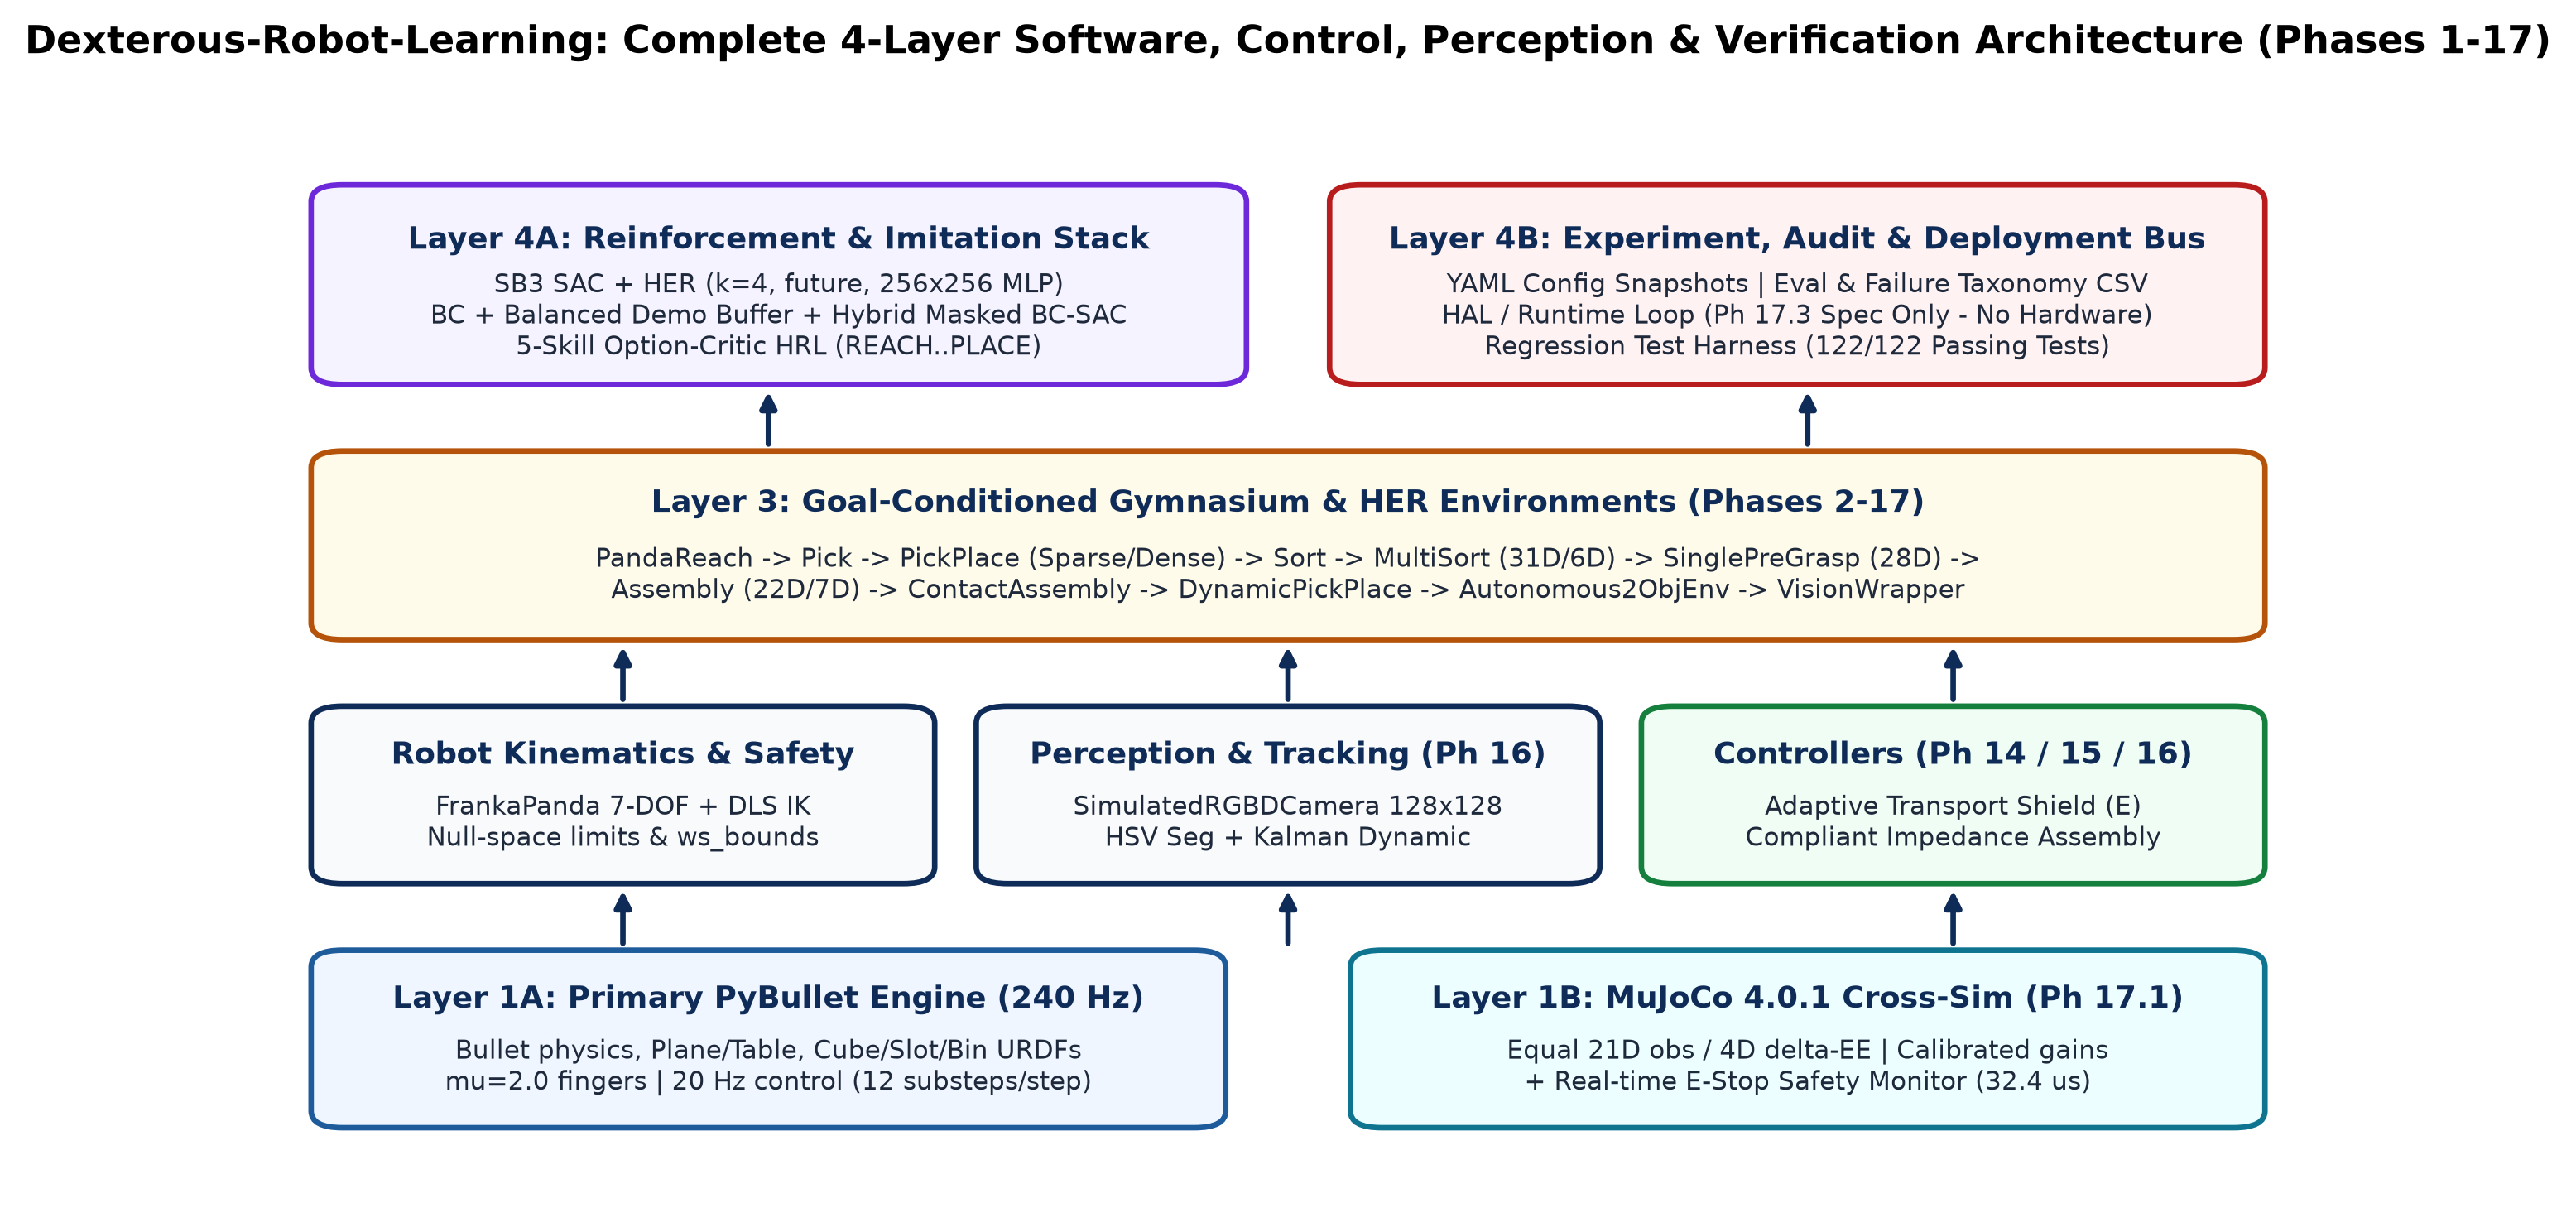
\includegraphics[width=0.92\linewidth]{publication/architecture_diagrams/arch_01_system_stack_ph1_to_17.png}\caption{Figure 1.1: Four-layer software, kinematics, control, perception, and verification stack unifying Phases 1-17.}\end{figure}
\begin{figure}[htbp]\centering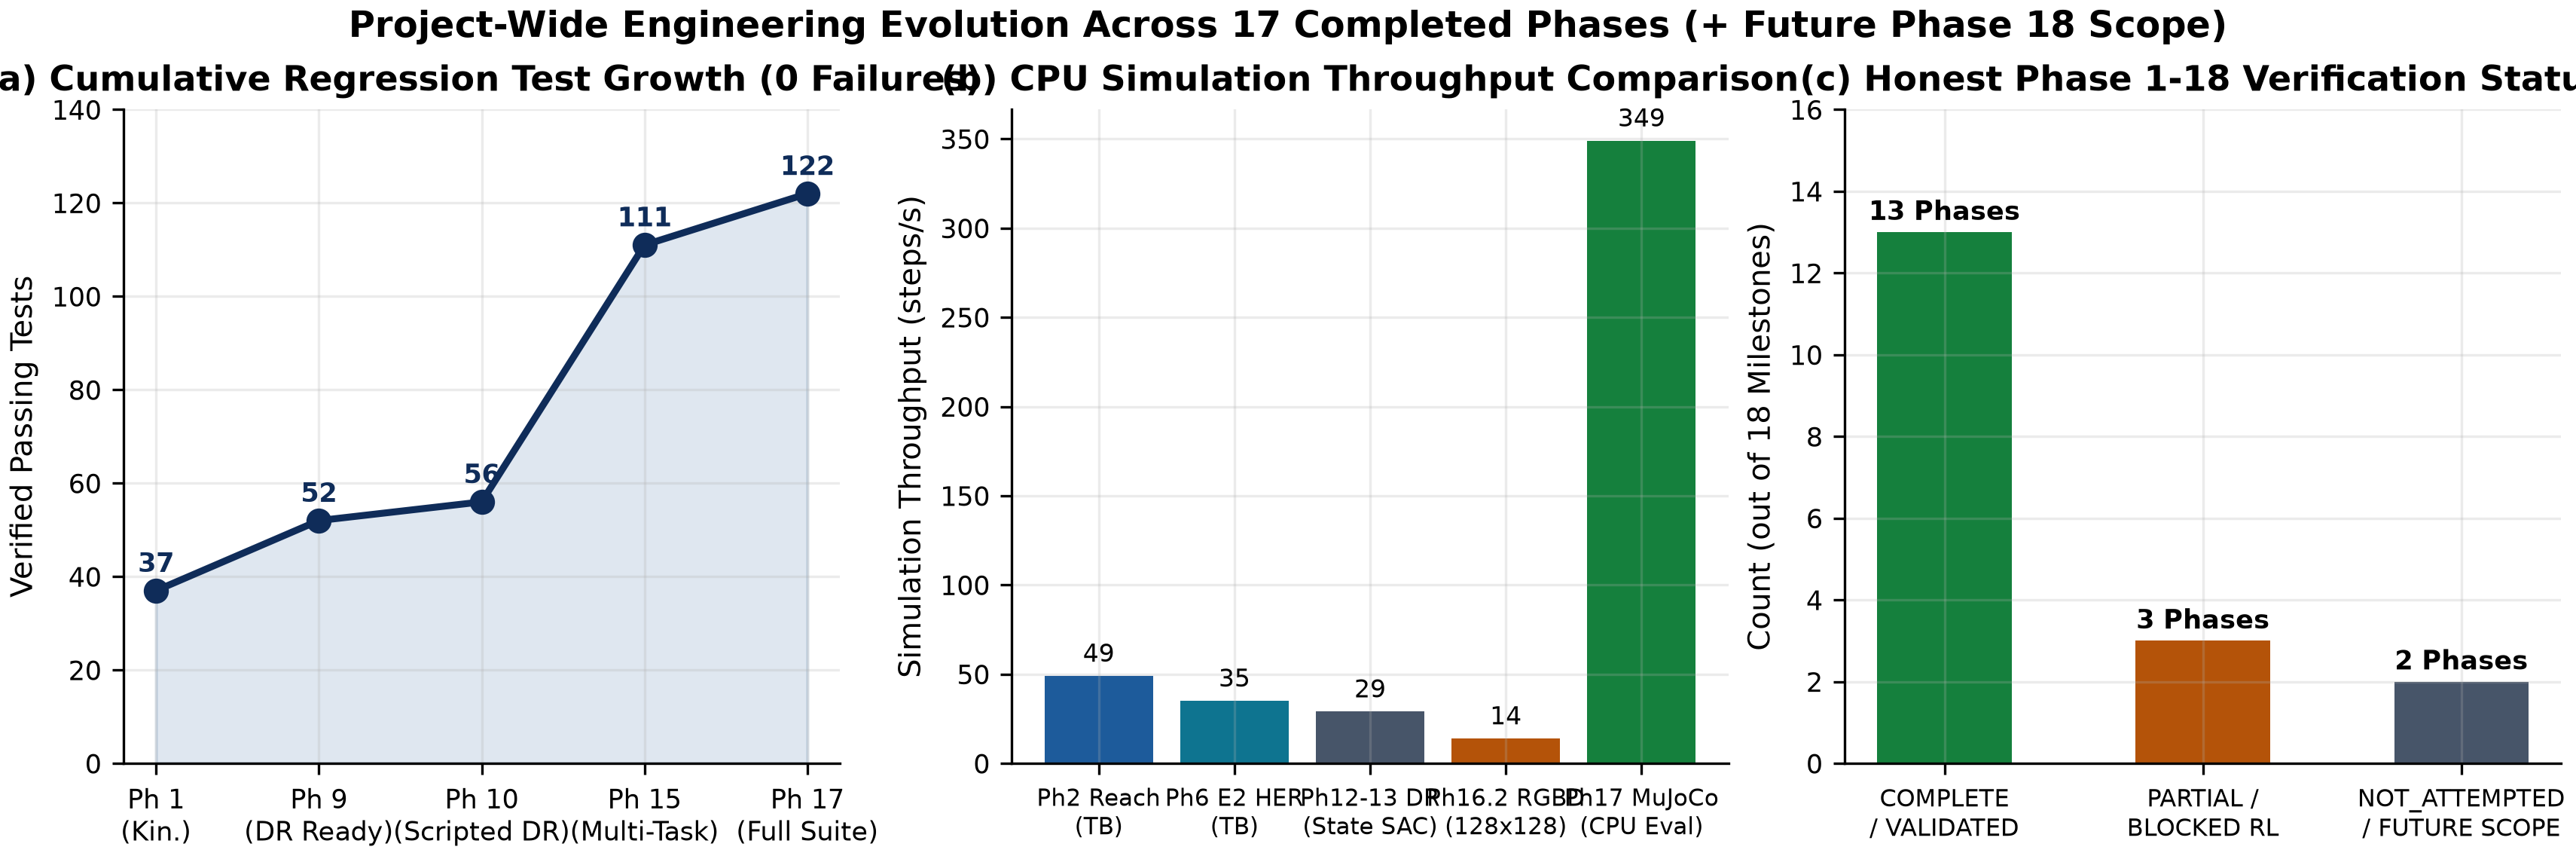
\includegraphics[width=0.92\linewidth]{publication/figures_2d/fig10_project_timeline_tests_throughput.png}\caption{Figure 1.2: Regression suite scaling (37 -> 122 passing tests), CPU step throughput comparison, and Phase 1-18 completion scorecard.}\end{figure}
\section{1.3 Hyperparameter and Environment Configuration Evolution}
Table 1.1 documents the exact evolution of YAML hyperparameters preserved across configs/*.yaml from early 10k sparse benchmarks (lr=1e-3, gamma=0.95, tau=0.05) to tuned long-horizon BC-SAC and assembly stabilization regimes (lr=3e-4 -> 1e-4, gamma=0.98, tau=0.005, extended learning\_starts up to 2,500 steps).

\begin{longtable}{l l l l l l l l}\caption{Table 1.1: Verbatim YAML Hyperparameter Matrix Across Key Phase Configurations}\\\toprule
Config File & Max Steps & LR & Gamma & Tau & Buffer & Budget & Learn Starts \\ \midrule \endhead
reach.yaml & 50 & 0.001 & 0.95 & 0.05 & 100000 & 10000 & default \\
pick.yaml & 100 & 0.001 & 0.95 & 0.05 & 100000 & 10000 & default \\
pick\_place\_her.yaml & 100 & 0.001 & 0.95 & 0.05 & 100000 & 10000 & default \\
pick\_place\_dr\_physics.yaml & 100 & 0.001 & 0.95 & 0.05 & 1000000 & 5000 & 250 \\
sort.yaml & 150 & 0.001 & 0.95 & 0.05 & 1000000 & 10000 & 200 \\
multi\_sort.yaml & 300 & 0.001 & 0.95 & 0.05 & 1000000 & 10000 & 350 \\
assembly.yaml & 200 & 0.001 & 0.95 & 0.05 & 1000000 & 10000 & 250 \\
multi\_sort\_phase15\_5B2.yaml & 80 & 0.0003 & 0.98 & 0.005 & 100000 & 5000 & 500 \\
multi\_sort\_phase15\_5B8.yaml & 80 & 0.0001 & 0.98 & 0.005 & 100000 & 10000 & 2500 \\
assembly\_phase15\_3.yaml & 120 & 0.0003 & 0.98 & 0.005 & 100000 & 5000 & 1000 \\
\bottomrule \end{longtable}
\section{1.4 Hardware Compute Envelope and Single-Process Determinism}
Every training and diagnostic campaign across Phases 0 through 17 ran exclusively under CPU-only PyTorch with single-process PyBullet physics stepping (timeStep = 1/240 s, 12 internal solver substeps per 20 Hz agent action step, yielding 0.05 s effective control period). No GPU CUDA acceleration or multi-worker VecEnv parallelism was utilized. Measurements extracted from archived TensorBoard logs show PyBullet state-based training throughput typically ranged between 18 and 49 steps/s depending on replay buffer warmup, multi-object collision count, and HER virtual relabeling ratio (k=4). Adding 128x128 tiny-renderer RGB-D camera capture in Phase 16.2 reduced closed-loop throughput to ~13.9 steps/s (2,000 steps in 143.54 s), whereas MuJoCo 4.0.1 C-engine evaluation in Phase 17.1 reached ~349 steps/s.

On Windows, concurrent imports of PyTorch (torch) and SciPy/NumPy binary wheels triggered Intel OpenMP runtime conflicts (OMP: Error \#15: Initializing libiomp5md.dll, recorded as ERR-011 during Phase 16.2). All benchmark scripts and automated regression suites isolate execution inside .conda-env/python.exe with KMP\_DUPLICATE\_LIB\_OK=TRUE and deterministic random seed injection across NumPy, PyTorch, and PyBullet spawn samplers.

\begin{longtable}{l l l l l}\caption{Table 1.3: Verified Core Canonical 10D/16D PickPlace Observation Tensor Layout}\\\toprule
Index Slice & Tensor Field & Dim & Physical Unit \& Semantics & Frame \\ \midrule \endhead
obs[0:3] & ee\_pos & 3 & Panda grasptarget Link 11 Cartesian XYZ (m) & World Base \\
obs[3] & gripper\_width & 1 & Sum of finger joints 9+10 opening [0.00, 0.08] (m) & Gripper \\
obs[4:7] & obj\_pos & 3 & Manipulated cube center-of-mass XYZ (m) & World Base \\
obs[7:10] & obj\_vel & 3 & Linear cube velocity [vx, vy, vz] (m/s) & World Base \\
achieved\_goal & ag & 3 & Cube XYZ (PickPlace) or EE XYZ (Reach) (m) & World Base \\
desired\_goal & dg & 3 & Target placement / bin XYZ coordinate (m) & World Base \\
\bottomrule \end{longtable}
\begin{longtable}{l l l l l}\caption{Table 1.2: Complete Historical Phase 0-17 Registry \& Provenance Classification (historical\_phase\_registry.json)}\\\toprule
Phase & Milestone Title & Period / Commit & Status & Evidence Class \\ \midrule \endhead
0 & Project Initialization \& Infrastruct & 2026-10-03 (git comm & COMPLETE & SOURCE\_VERIFIED \\
1 & Franka Panda Kinematics, PyBullet Fo & 2026-10-03 (git comm & COMPLETE & SOURCE\_VERIFIED \\
2 & Goal-Conditioned Manipulation Enviro & Oct 2026 (pre-commit & COMPLETE & REPORT\_VERIFIED \\
3 & SAC + HER RL Training, Evaluation \&  & Oct 2026 (recovered  & COMPLETE & LOG\_VERIFIED \\
4 & Object Grasping Abstraction \& PandaP & Oct 2026 (recovered  & COMPLETE & SOURCE\_VERIFIED \\
5 & Reach/Pick Exploration \& Early Contr & Oct-Nov 2026 & PARTIALLY\_COMPLETE & HISTORICALLY\_REPORTED \\
6 & Pick \& Place Environment, HER Compar & Oct-Nov 2026 (experi & COMPLETE & LOG\_VERIFIED \\
7 & Color-Conditioned Dynamic Sorting Be & Oct-Nov 2026 (docs/e & COMPLETE & LOG\_VERIFIED \\
8 & Sequential Multi-Object Sorting \& Or & Oct-Nov 2026 (docs/e & COMPLETE & LOG\_VERIFIED \\
9 & Full-System Diagnostic Audit \& Lazy  & Nov 2026 (docs/phase & COMPLETE & REPORT\_VERIFIED \\
10 & Deterministic Domain Randomization E & Nov 2026 (docs/phase & COMPLETE & REPORT\_VERIFIED \\
11 & 100k Sparse DR Matrix \& Diagnostic I & Nov 2026 (docs/phase & COMPLETE & LOG\_VERIFIED \\
12 & 1M-Step Dense SAC+HER Scaling Breakt & Nov 2026 (docs/phase & COMPLETE & LOG\_VERIFIED \\
13 & Dense Domain Randomization (DR1/DR2/ & 2026-11-03 to 2026-1 & COMPLETE & LOG\_VERIFIED \\
14 & Zero-Retraining Adaptive Control Sui & 2026-11-10 (results/ & COMPLETE & LOG\_VERIFIED \\
15 & Sim-to-Real Sensitivity (15.1), Mult & 2026-11-10 to 2026-1 & PARTIALLY\_COMPLETE & SOURCE\_VERIFIED \\
16 & Hierarchical RL, Oblique RGB-D Visio & 2026-11-11 to 2026-1 & COMPLETE & SOURCE\_VERIFIED \\
17 & MuJoCo Cross-Simulator Validation, S & 2026-11-12 (results/ & PARTIALLY\_COMPLETE & SOURCE\_VERIFIED \\
\bottomrule \end{longtable}
\chapter{Chapter 2: Foundation Kinematics, PyBullet Physics, Reach, and Pick (Phases 1-4)}
\section{2.1 Phase 0-1: Franka Emika Panda Kinematics and Cartesian Controller}
Earliest repository commits (3a345f3, a5cc06b, and 7ad9848 on 2026-10-03) built PyBulletSim and FrankaPanda atop franka\_panda/panda.urdf. Arm joints [0..6] operate under motor torque saturation [87, 87, 87, 87, 12, 12, 12] N*m with 0.04 linear and angular damping, while finger joints [9, 10] actuate up to 25 N across a symmetric [0.00, 0.08] m parallel-jaw span. Control commands dx in R^3 (bounded to +-0.05 m per 20 Hz cycle inside x=[0.25, 0.75], y=[-0.35, 0.35], z=[0.02, 0.50] m) resolve joint increments through damped least-squares inverse kinematics (lambda=0.05, max\_iter=100, tol=1e-4, Equation (1)). Five deterministic validation waypoints confirmed end-effector error between 0.7 mm and 4.5 mm alongside 37/37 unit tests in 4.71 s.

\begin{figure}[htbp]\centering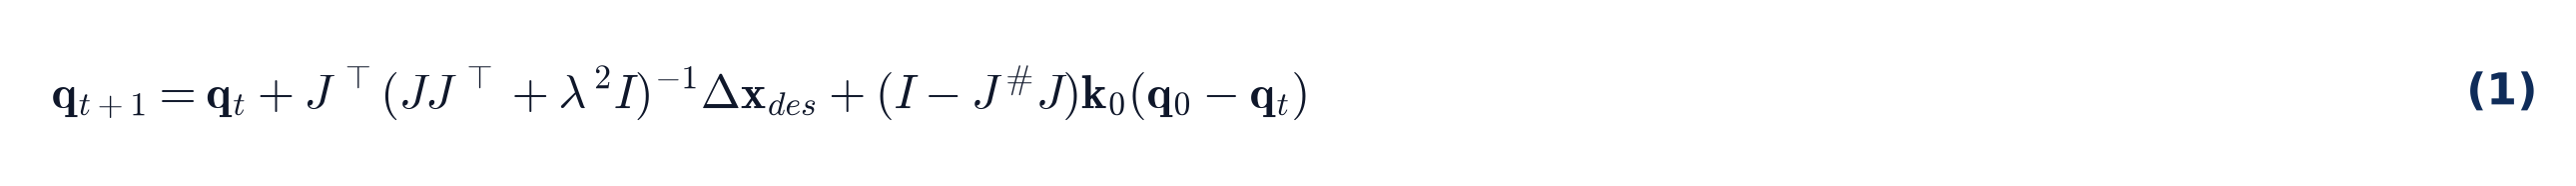
\includegraphics[width=0.92\linewidth]{publication/equations/eq_01.png}\caption{Equation (1): Damped least-squares IK with null-space neutral posture regularization.}\end{figure}
\begin{figure}[htbp]\centering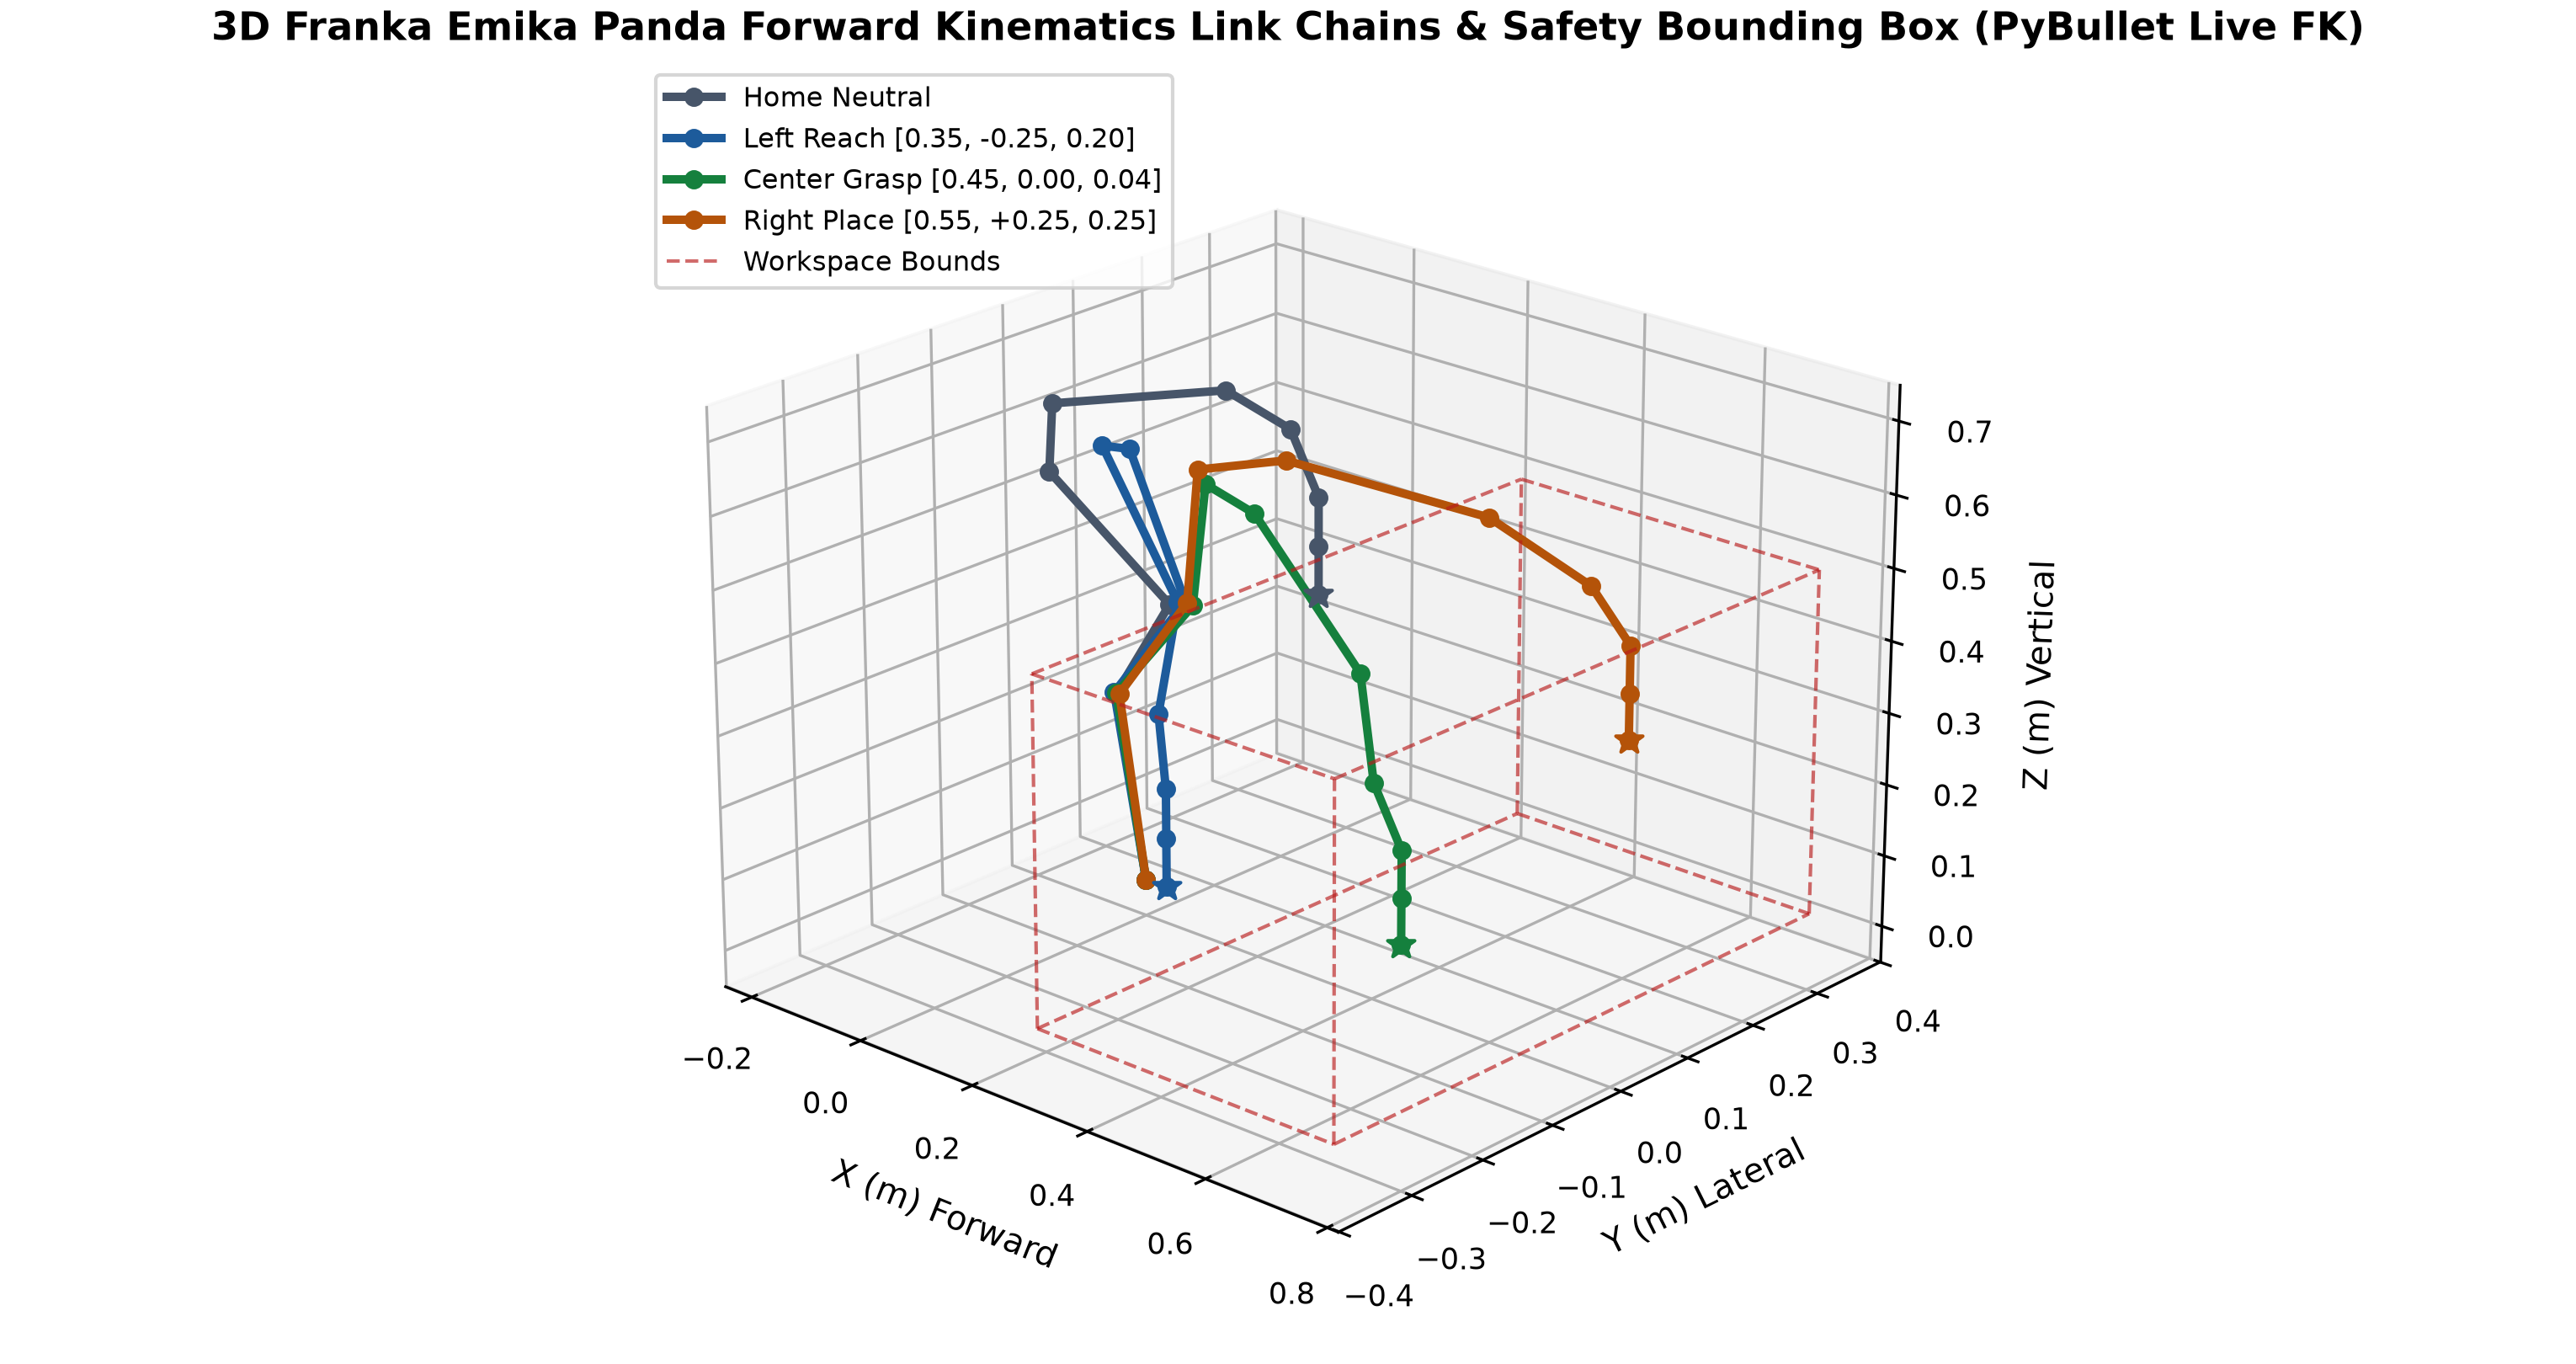
\includegraphics[width=0.92\linewidth]{publication/figures_3d/fig3d_01_panda_fk_and_workspace.png}\caption{Figure 2.1: Live PyBullet 3D forward-kinematic link chains for FrankaPanda inside workspace bounds.}\end{figure}
\section{2.2 Phases 2-4: Reach, Pick, and Reconstructed Early TensorBoard Diagnostics}
Phase 2 (PandaReachEnv, 4D obs + 6D goals, 50 steps) and Phase 3 (SB3 SAC+HER callback harness) produced three reach event streams: logs/reach\_sac/SAC\_1 and SAC\_2 contain 0 scalar events (aborted pre-warmup launches), whereas SAC\_3 logged 10,000 steps. Actor loss climbed monotonically (-9.127 -> +19.518) as entropy collapsed (0.907 -> 0.002), while rollout success hit 1.0\% against 0\% deterministic evaluation (-50.0 reward). Phase 4 (PandaPickEnv, target\_altitude=0.20 m, 100 steps) mirrored this trajectory (actor\_loss -14.331 -> +20.005, ent\_coef 0.742 -> 0.000, eval -100.0). Scripted controllers solved Reach at Step 6 and Pick at Step 67. Standalone Phase 5 reports do not exist in the repository and remain marked NOT\_RECOVERABLE.

\begin{figure}[htbp]\centering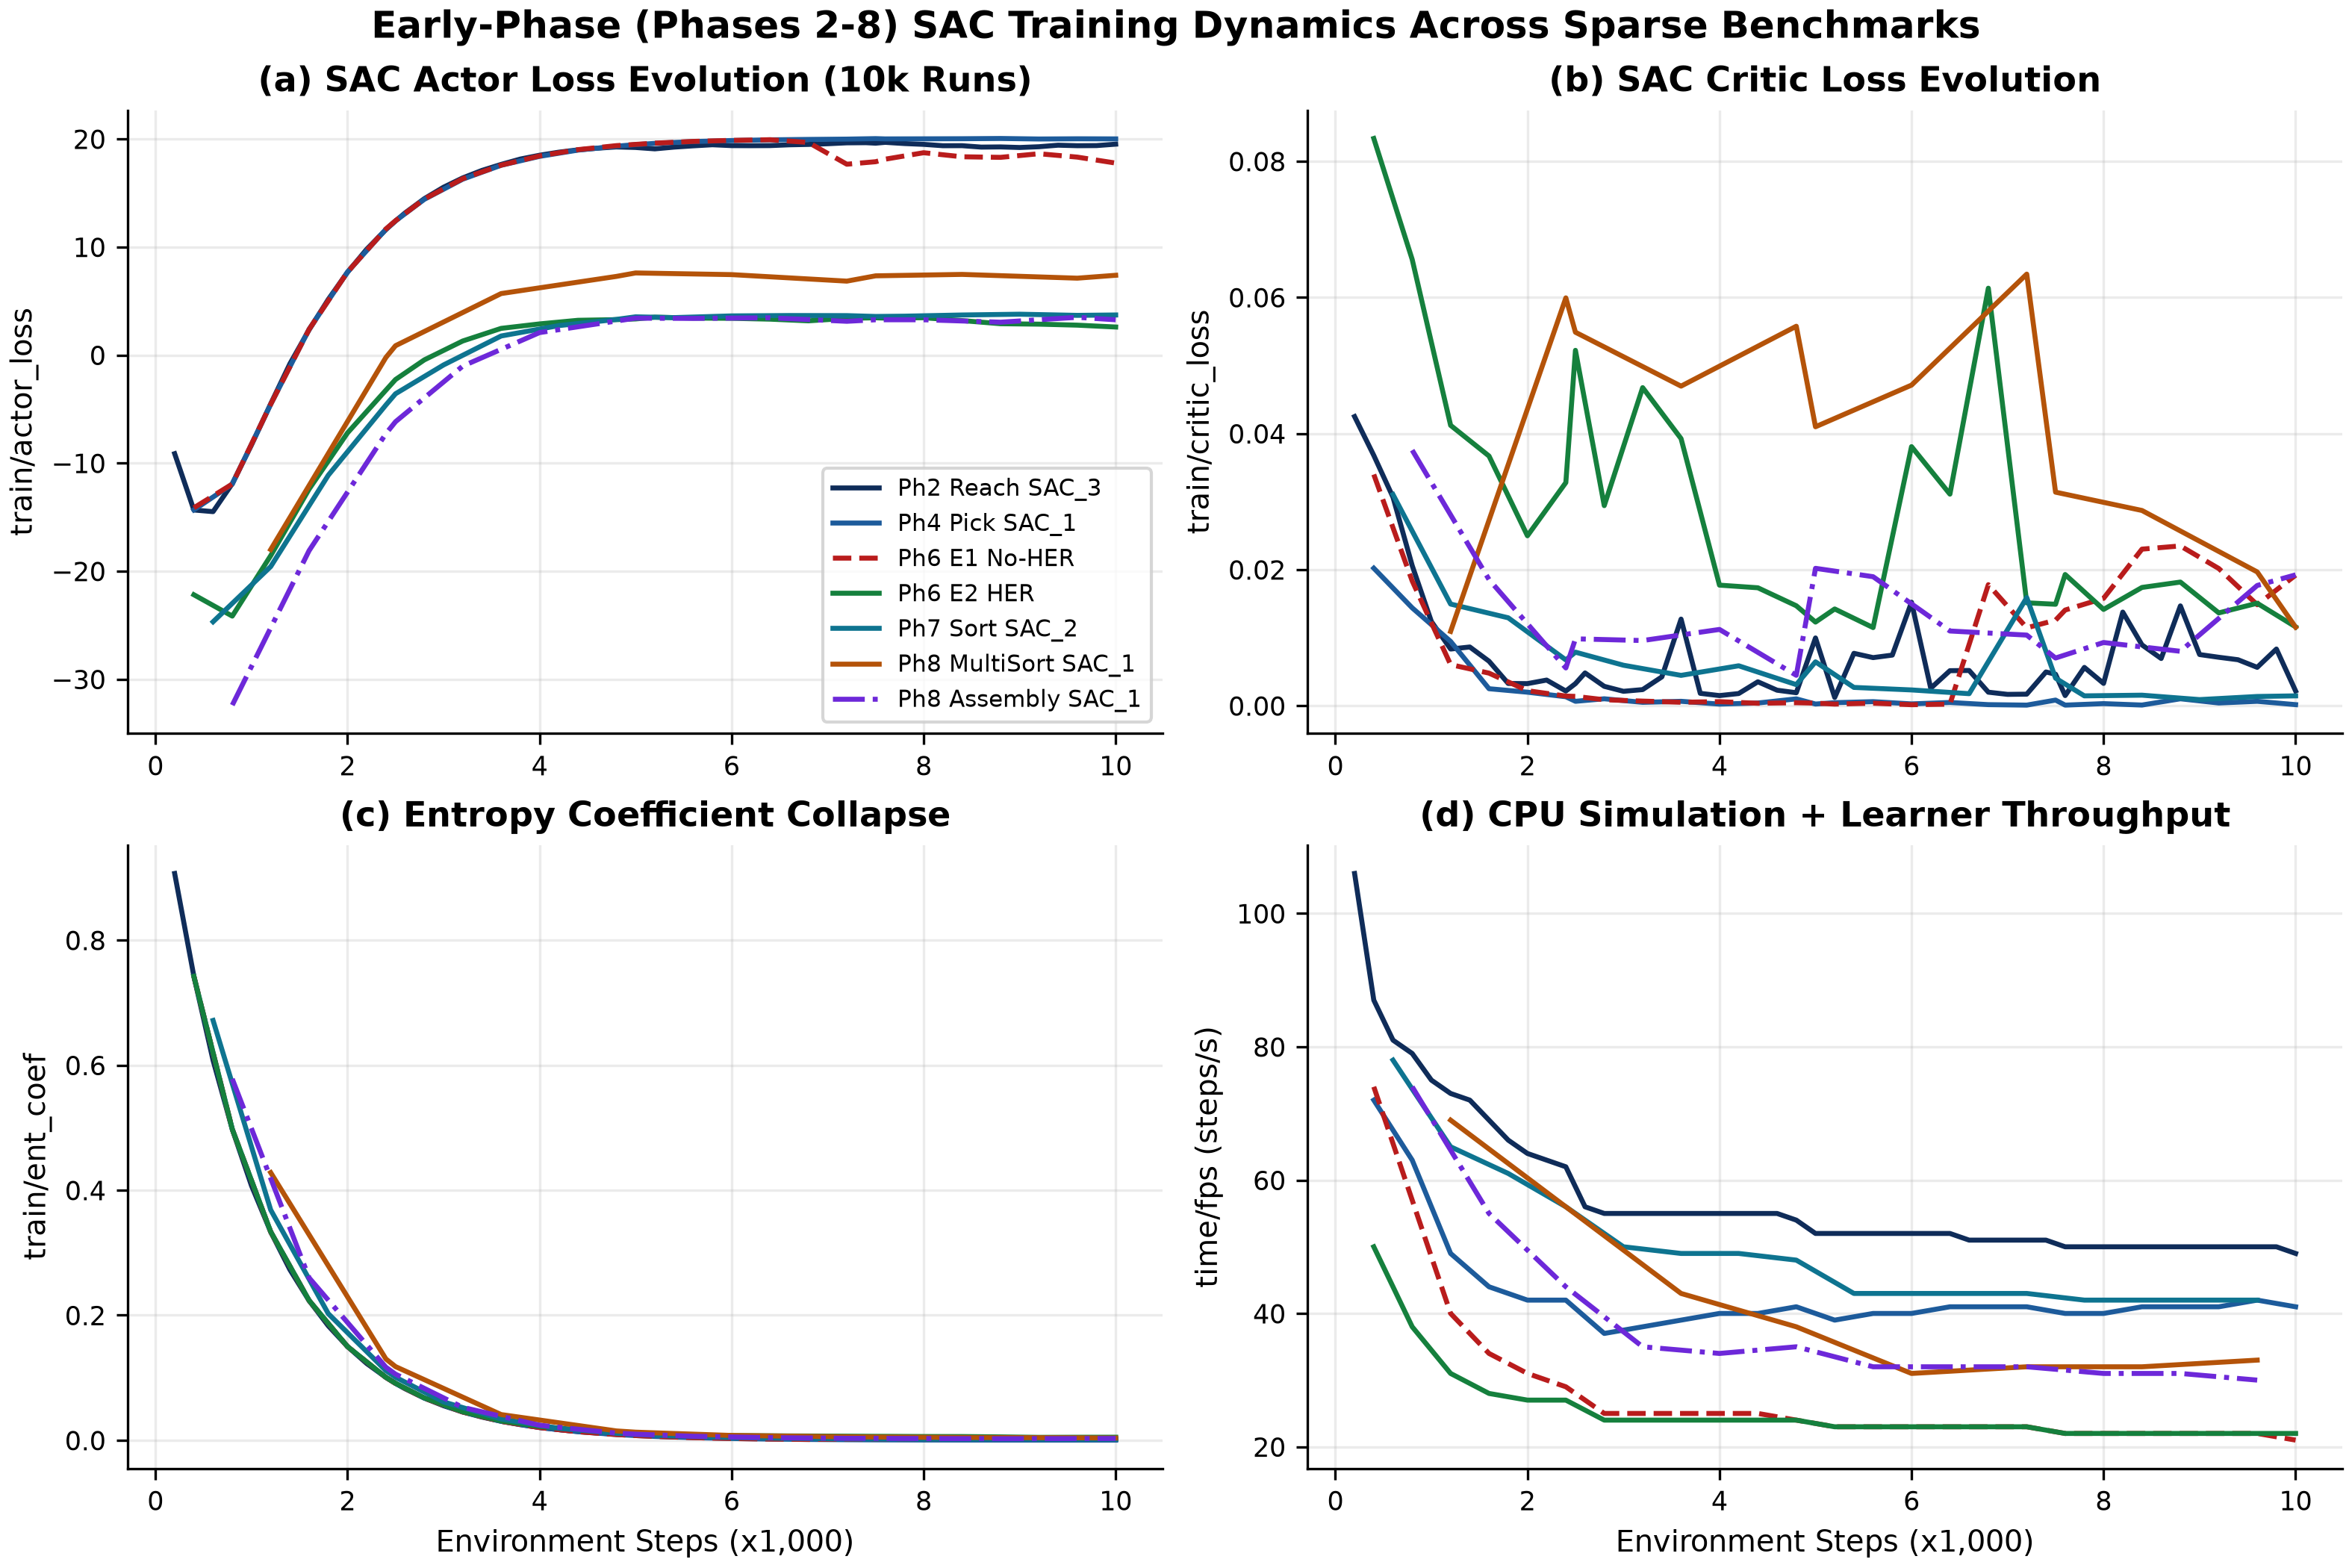
\includegraphics[width=0.92\linewidth]{publication/figures_2d/fig01_early_tb_diagnostics.png}\caption{Figure 2.2: Exact TensorBoard training metrics across Phases 2-8 (actor loss, critic loss, entropy decay, and CPU FPS).}\end{figure}
\begin{longtable}{l l l l l l}\caption{Table 2.1: Reconstructed Early Phase TensorBoard \& Scripted Baseline Comparison (Exact Measurements)}\\\toprule
Run ID & Env / Steps & Actor Loss Trajectory & Ent Coef Decay & FPS & Outcome / Baseline \\ \midrule \endhead
logs/reach\_sac/SAC\_3 & Reach / 50 & -9.127 -> +19.518 & 0.907 -> 0.002 & 106 -> 49 & Rollout 1\%; Eval -50; Script Step 6 \\
logs/pick\_sac/SAC\_1 & Pick / 100 & -14.331 -> +20.005 & 0.742 -> 0.000 & 72 -> 41 & Eval -100; Script Step 67 \\
E1\_no\_her/SAC\_1 & PickPlace / 100 & -14.135 -> +17.767 & 0.875 -> 0.000 & 74 -> 21 & 7.7 colls/ep; Eval -100 \\
E2\_her/SAC\_1 & PickPlace / 100 & -22.183 -> +2.594 & 0.892 -> 0.001 & 81 -> 35 & 0.0 colls; Rollout 2\%; Script Step 74 \\
logs/sort/SAC\_2 & Sort / 150 & -24.686 -> +3.710 & 0.870 -> 0.001 & 80 -> 30 & Eval -150; Script Step 79 \\
logs/multi\_sort/SAC\_1 & MultiSort / 300 & -18.002 -> +7.383 & 0.869 -> 0.001 & 54 -> 18 & Eval -600; Script Step 209 \\
logs/assembly/SAC\_1 & Assembly / 200 & -32.398 -> +3.264 & 0.885 -> 0.001 & 57 -> 21 & Eval -200; Script Step 143 \\
\bottomrule \end{longtable}
\section{2.3 Algorithmic Control Pipeline \& Why 10k Sparse Runs Collapsed}
\begin{quote}\small\textbf{Algorithm Summary}\\Algorithm 1: FrankaPanda Damped Least-Squares Cartesian Step Controller (src/robots/panda.py) \\ 1. Receive normalized policy delta action a\_t in [-1, 1]^4 -> dx = clip(a[0:3], -1, 1) * 0.05 m. \\ 2. Query current EE link 11 position p\_t and compute clipped target p\_des = clip(p\_t + dx, ws\_min, ws\_max). \\ 3. Solve PyBullet DLS IK (lambda=0.05, max\_iter=100, residual\_tol=1e-4) biased toward neutral joints q\_0. \\ 4. Map scalar gripper command a[3] -> jaw aperture target in [0.00, 0.08] m (max motor force 25 N). \\ 5. Execute 12 PyBullet physics substeps at dt = 1/240 s using joint position/velocity PD actuators.\end{quote}

Analyzing Phase 2-4 logs alongside Algorithm 1 explains why all early 10k RL runs ended at 0\% deterministic evaluation even on Reach (50-step horizon) and Pick (100-step horizon). Stable-Baselines3 SAC initializes entropy coefficient alpha via a learned log-parameter tuned against target entropy -dim(A) = -4.0. In sparse reward landscapes where zero positive rewards (+0.0) are encountered during the first few thousand random samples, Q-targets remain uniformly constant (-1 / (1 - gamma) * const), causing policy entropy to shrink rapidly (0.907 -> 0.002 in Reach SAC\_3; 0.742 -> 0.000 in Pick SAC\_1) before meaningful spatial workspace coverage can occur.

\chapter{Chapter 3: Pick-and-Place, Hindsight Experience Replay, Sorting, and Early Assembly (Phases 5-8)}
\section{3.1 Phase 6: HER Ablation and Finger Friction Physics Fix (ERR-001)}
Phase 6 implemented PandaPickPlaceEnv and revealed ERR-001: low default tangential friction in Bullet allowed gripped 0.10 kg cubes to slide downward during liftoff. Configuring lateralFriction=2.0 and spinningFriction=0.1 on finger links 9 and 10 inside FrankaPanda.\_\_init\_\_ stabilized scripted pick-and-place at Step 74. Comparing E1 (No-HER SAC) vs E2 (SAC+HER, k=4 future, Equations (2)-(7)) across 10k smoke runs showed HER curbed Q-value blowup (actor\_loss +2.594/+3.061 vs +17.767) and reduced table collisions from 7.7/ep to 0.0/ep.

\begin{figure}[htbp]\centering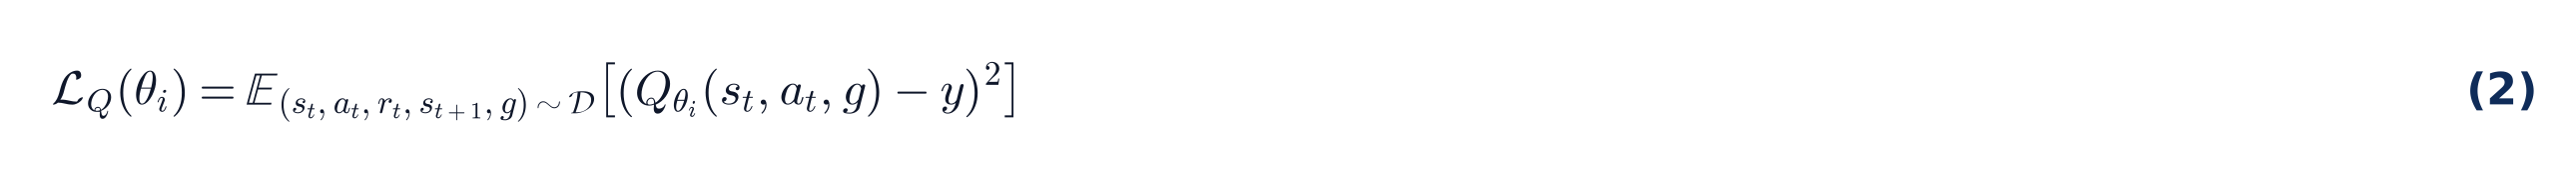
\includegraphics[width=0.92\linewidth]{publication/equations/eq_02.png}\caption{Equation (2): Double Q-critic MSE loss with clipped target values.}\end{figure}
\begin{figure}[htbp]\centering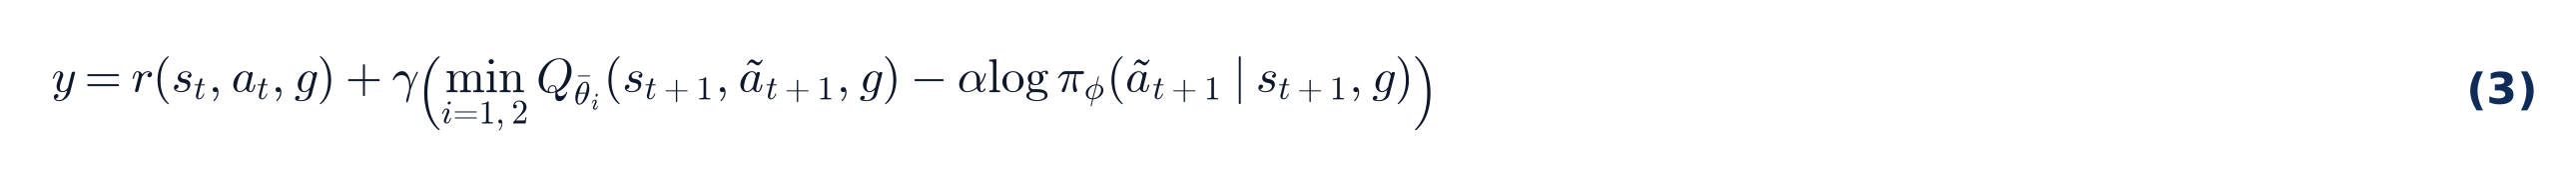
\includegraphics[width=0.92\linewidth]{publication/equations/eq_03.png}\caption{Equation (3): Soft Bellman target including entropy bonus.}\end{figure}
\begin{figure}[htbp]\centering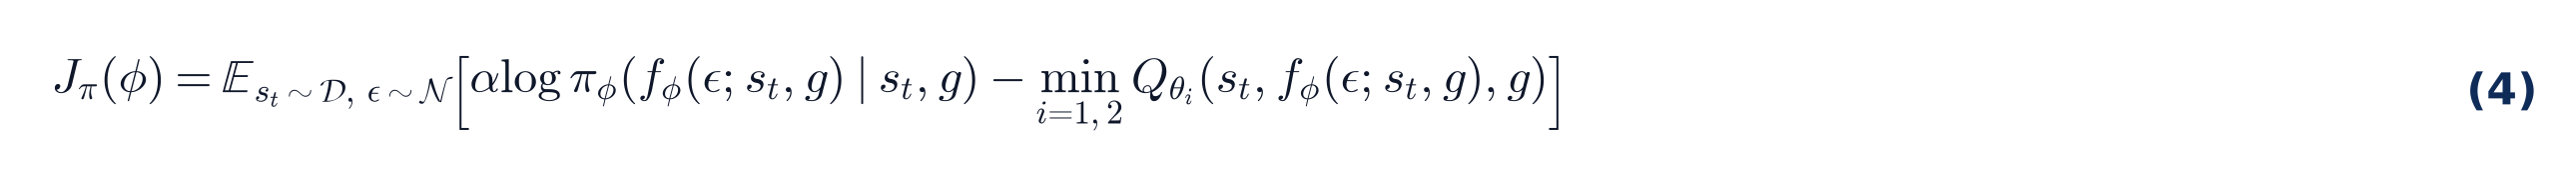
\includegraphics[width=0.92\linewidth]{publication/equations/eq_04.png}\caption{Equation (4): Reparameterized SAC policy gradient objective.}\end{figure}
\begin{figure}[htbp]\centering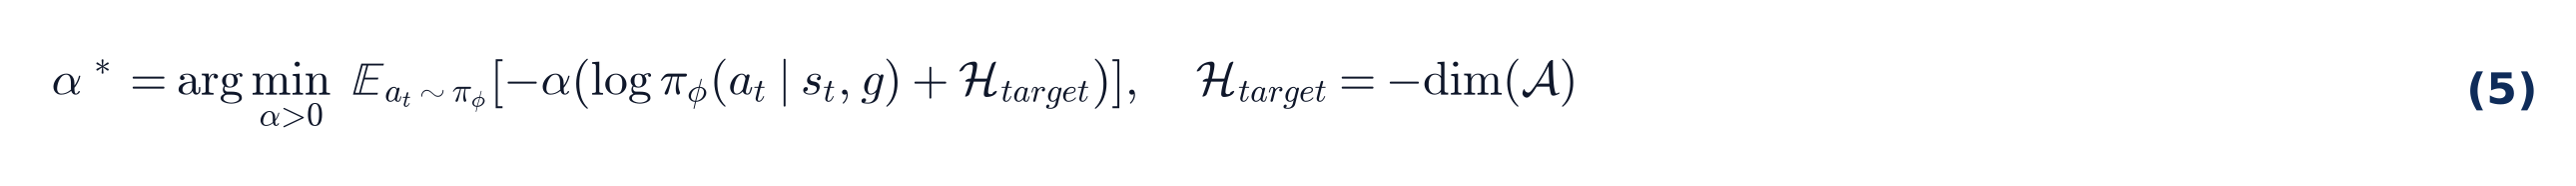
\includegraphics[width=0.92\linewidth]{publication/equations/eq_05.png}\caption{Equation (5): Lagrange dual update for automatic entropy coefficient alpha.}\end{figure}
\begin{figure}[htbp]\centering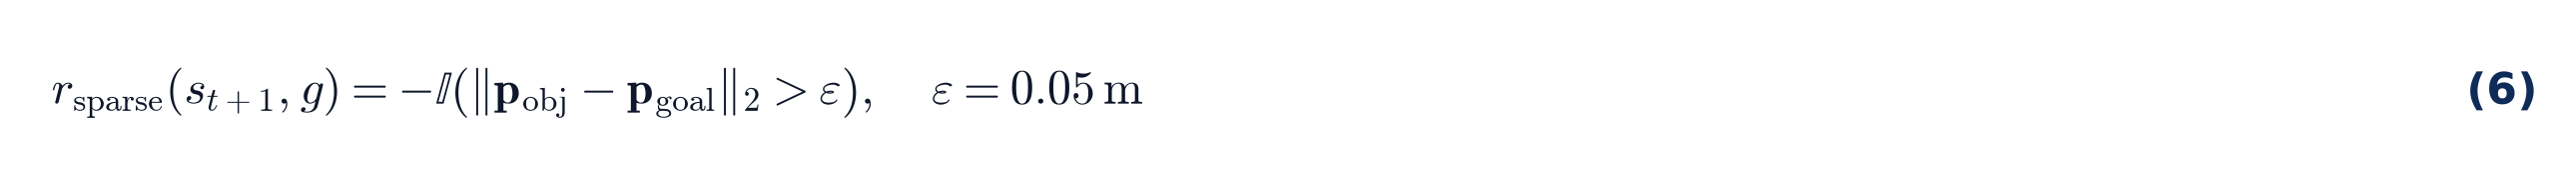
\includegraphics[width=0.92\linewidth]{publication/equations/eq_06.png}\caption{Equation (6): Binary sparse Euclidean tolerance reward (-1 outside 5 cm).}\end{figure}
\begin{figure}[htbp]\centering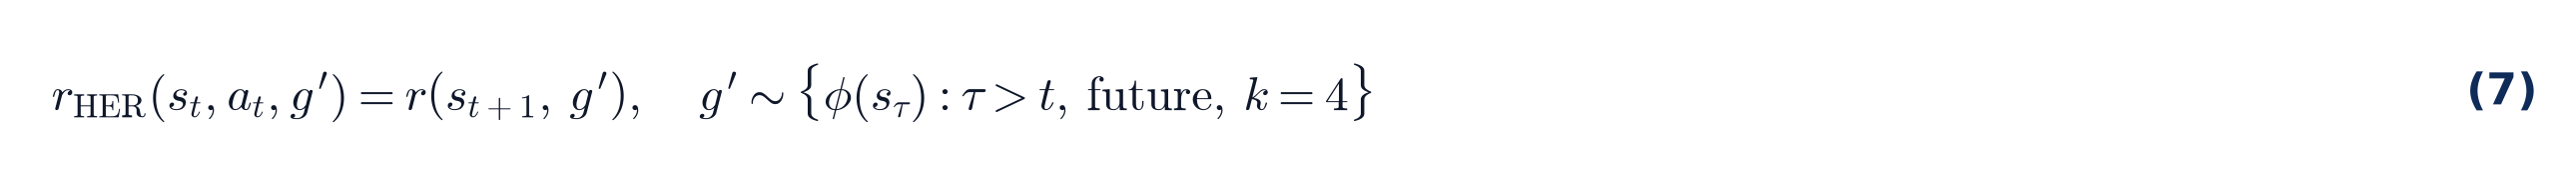
\includegraphics[width=0.92\linewidth]{publication/equations/eq_07.png}\caption{Equation (7): Future-strategy HER virtual goal relabeling rule (k=4).}\end{figure}
\begin{figure}[htbp]\centering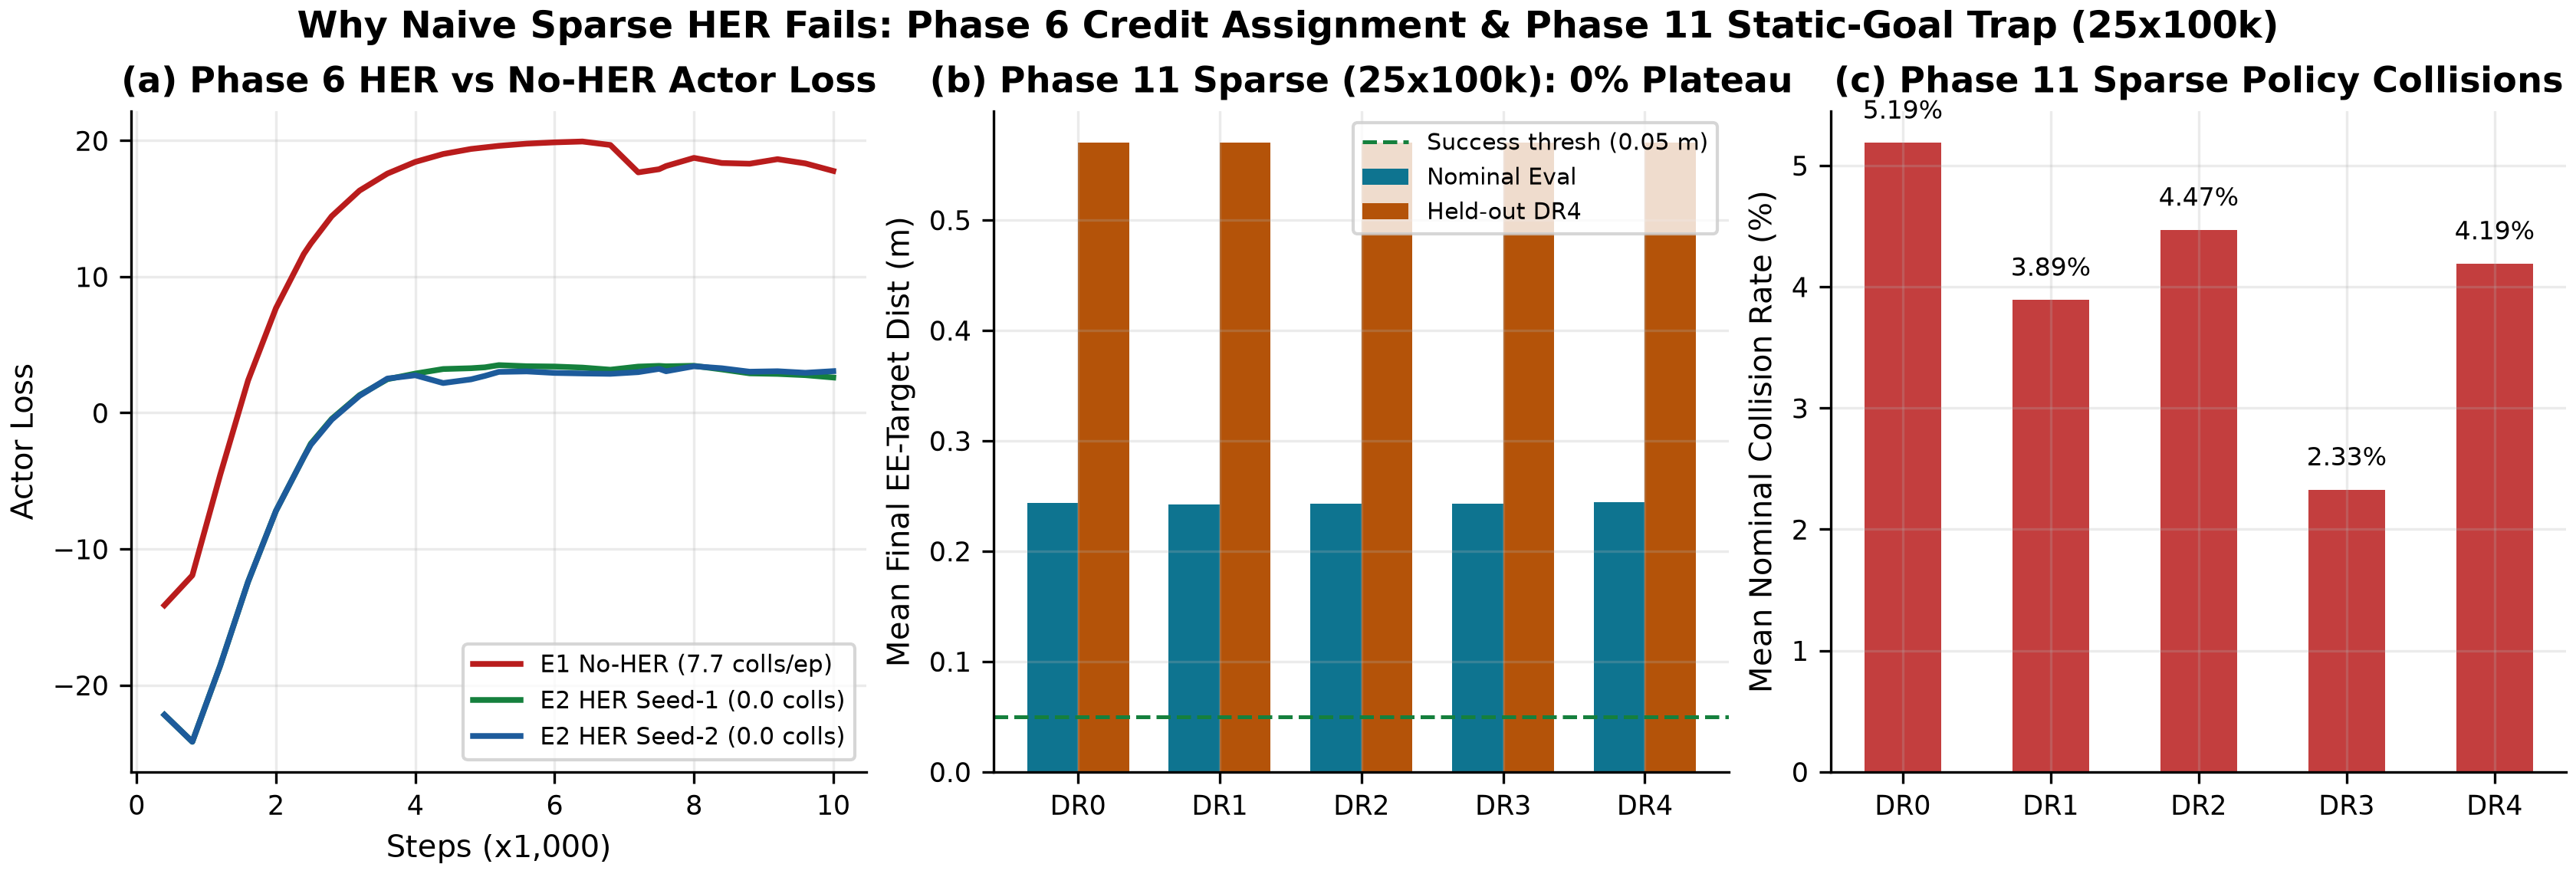
\includegraphics[width=0.92\linewidth]{publication/figures_2d/fig02_her_vs_noher_sparse_vs_dense.png}\caption{Figure 3.1: (a) Phase 6 HER regularization effect; (b-c) Phase 11 25-run sparse failure distance and collision breakdown.}\end{figure}
\section{3.2 Phases 7-8: Color Sorting, Dual-Cube Multi-Sorting, and Assembly Prototyping}
Phase 7 added color-matched SortingBin placement (PandaSortEnv, 150 steps, scripted Step 79). Phase 8 scaled to two sequential objects in PandaMultiSortEnv (31D observation, 6D desired\_goal, 300 steps, scripted Step 209) and 5D orientation-aware peg-in-slot control [dx, dy, dz, dyaw, gripper] in PandaAssemblyEnv (22D observation, 7D goal, 200 steps, scripted Step 143). Brief 10k sparse RL evaluations remained uniformly unsolved (-150, -600, -200 mean return).

\section{3.3 Algorithmic Formalism: Off-Policy SAC with Future-Strategy HER}
\begin{quote}\small\textbf{Algorithm Summary}\\Algorithm 2: Goal-Conditioned SAC + HER Replay Update (Phases 3-13) \\ 1. Collect trajectory tau = (s\_0, a\_0, ..., s\_T, dg) under stochastic actor pi\_phi(a | s, dg). \\ 2. Store original transition (s\_t, a\_t, s\_{t+1}, r(s\_{t+1}, dg), dg) into HerReplayBuffer. \\ 3. For k = 4 virtual samples per transition: draw future step tau > t, set virtual goal g' = ag\_tau. \\ 4. Recompute task reward r' = compute\_reward(ag\_{t+1}, g', info) cleanly via vectorized NumPy hook. \\ 5. Update Twin Critics Q\_theta1,2 (Eq. 2-3), Reparameterized Actor pi\_phi (Eq. 4), and Alpha (Eq. 5).\end{quote}

A critical structural discovery occurred in Phase 6 (ERR-001) and scaled sharply in Phases 7-8. On PandaMultiSortEnv (31D obs, 6D dual-object goals), HER relabeling faces combinatorial coupling: shifting cube A accidentally alters cube A's final coordinate, yet if cube B remains undisturbed, virtual goals referencing only touched trajectories fail to decouple independent object sub-goals within a 300-step horizon unless explicit stage decomposition or PreGrasp gating is enforced (Phase 15.2.5A).

\chapter{Chapter 4: System Audit, Domain Randomization, and Sparse HER Failure Forensics (Phases 9-11)}
\section{4.1 Phases 9-10: Lazy Client Repair and Five-Tier Domain Randomization}
Phase 9 resolved ERR-002 (deferred client\_id injection in PandaAssemblyEnv.reset()) raising verified passing unit tests to 52/52 (6.47 s). Phase 10 formalized physics/geometry randomization R0..R4, passing 56/56 tests and achieving scripted DR baseline rates of 90\% (R0), 85\% (R1), 100\% (R2), 85\% (R3), and 75\% (R4) across 20 episodes per condition.

\section{4.2 Phase 11: Complete 25-Run (2.5M-Step) Sparse Evaluation Audit}
Phase 11 trained 25 independent sparse SAC+HER agents (5 DR tiers x seeds 42..46, 100k steps each) and evaluated all 25 models on 100 Nominal and 100 Held-Out DR4 episodes (5,000 total episodes, Table 4.1). All 25 runs scored 0.0\% task completion (mean held-out distance 0.5698 m, nominal ~0.243 m). Phase 11.5 isolated ERR-003 (the HER Static-Goal Trap): because sparse exploration rarely touched the cube, future goals repeated initial resting coordinates, reinforcing passive hovering. Phase 11.9 proved transport itself was straightforward (100\% in 40-50k on pre-grasped TransportDiagnosticEnv), while 11.10b reached 28\% Reach / 23\% Grasp @ 225k.

\begin{longtable}{l l l l l l l}\caption{Table 4.1: Complete 50-Row Phase 11 Sparse Evaluation Matrix (results/phase11\_final\_summary.csv)}\\\toprule
DR Tier & Seed & Eval Split & Success & Grasp & Mean Dist & Coll Rate \\ \midrule \endhead
DR0 & 42 & Held-out & 0.0\% & 0.0\% & 0.5698 m & 0.00\% \\
DR0 & 42 & Nominal & 0.0\% & 1.0\% & 0.2460 m & 18.33\% \\
DR0 & 43 & Held-out & 0.0\% & 0.0\% & 0.5698 m & 0.00\% \\
DR0 & 43 & Nominal & 0.0\% & 0.0\% & 0.2427 m & 2.51\% \\
DR0 & 44 & Held-out & 0.0\% & 0.0\% & 0.5698 m & 0.00\% \\
DR0 & 44 & Nominal & 0.0\% & 0.0\% & 0.2431 m & 0.62\% \\
DR0 & 45 & Held-out & 0.0\% & 0.0\% & 0.5698 m & 0.00\% \\
DR0 & 45 & Nominal & 0.0\% & 0.0\% & 0.2427 m & 1.15\% \\
DR0 & 46 & Held-out & 0.0\% & 0.0\% & 0.5698 m & 0.00\% \\
DR0 & 46 & Nominal & 0.0\% & 0.0\% & 0.2448 m & 3.32\% \\
DR1 & 42 & Held-out & 0.0\% & 0.0\% & 0.5698 m & 0.00\% \\
DR1 & 42 & Nominal & 0.0\% & 0.0\% & 0.2427 m & 0.00\% \\
DR1 & 43 & Held-out & 0.0\% & 0.0\% & 0.5698 m & 0.00\% \\
DR1 & 43 & Nominal & 0.0\% & 0.0\% & 0.2427 m & 2.16\% \\
DR1 & 44 & Held-out & 0.0\% & 0.0\% & 0.5698 m & 0.00\% \\
DR1 & 44 & Nominal & 0.0\% & 0.0\% & 0.2427 m & 8.28\% \\
DR1 & 45 & Held-out & 0.0\% & 0.0\% & 0.5698 m & 0.00\% \\
DR1 & 45 & Nominal & 0.0\% & 0.0\% & 0.2426 m & 0.00\% \\
DR1 & 46 & Held-out & 0.0\% & 0.0\% & 0.5698 m & 0.00\% \\
DR1 & 46 & Nominal & 0.0\% & 0.0\% & 0.2417 m & 9.01\% \\
DR2 & 42 & Held-out & 0.0\% & 0.0\% & 0.5698 m & 0.00\% \\
DR2 & 42 & Nominal & 0.0\% & 0.0\% & 0.2449 m & 5.55\% \\
DR2 & 43 & Held-out & 0.0\% & 0.0\% & 0.5698 m & 0.00\% \\
DR2 & 43 & Nominal & 0.0\% & 0.0\% & 0.2427 m & 1.17\% \\
DR2 & 44 & Held-out & 0.0\% & 0.0\% & 0.5698 m & 0.00\% \\
DR2 & 44 & Nominal & 0.0\% & 0.0\% & 0.2427 m & 2.95\% \\
DR2 & 45 & Held-out & 0.0\% & 0.0\% & 0.5698 m & 0.00\% \\
DR2 & 45 & Nominal & 0.0\% & 0.0\% & 0.2427 m & 4.25\% \\
DR2 & 46 & Held-out & 0.0\% & 0.0\% & 0.5698 m & 0.00\% \\
DR2 & 46 & Nominal & 0.0\% & 0.0\% & 0.2427 m & 8.42\% \\
DR3 & 42 & Held-out & 0.0\% & 0.0\% & 0.5698 m & 0.00\% \\
DR3 & 42 & Nominal & 0.0\% & 0.0\% & 0.2427 m & 0.16\% \\
DR3 & 43 & Held-out & 0.0\% & 0.0\% & 0.5698 m & 0.00\% \\
DR3 & 43 & Nominal & 0.0\% & 0.0\% & 0.2424 m & 2.80\% \\
DR3 & 44 & Held-out & 0.0\% & 0.0\% & 0.5698 m & 0.00\% \\
DR3 & 44 & Nominal & 0.0\% & 0.0\% & 0.2421 m & 0.66\% \\
DR3 & 45 & Held-out & 0.0\% & 0.0\% & 0.5698 m & 0.00\% \\
DR3 & 45 & Nominal & 0.0\% & 0.0\% & 0.2427 m & 2.87\% \\
DR3 & 46 & Held-out & 0.0\% & 0.0\% & 0.5698 m & 3.95\% \\
DR3 & 46 & Nominal & 0.0\% & 0.0\% & 0.2432 m & 5.14\% \\
DR4 & 42 & Held-out & 0.0\% & 0.0\% & 0.5698 m & 0.00\% \\
DR4 & 42 & Nominal & 0.0\% & 0.0\% & 0.2427 m & 6.66\% \\
DR4 & 43 & Held-out & 0.0\% & 0.0\% & 0.5698 m & 0.00\% \\
DR4 & 43 & Nominal & 0.0\% & 0.0\% & 0.2433 m & 2.30\% \\
DR4 & 44 & Held-out & 0.0\% & 0.0\% & 0.5698 m & 0.00\% \\
DR4 & 44 & Nominal & 0.0\% & 0.0\% & 0.2460 m & 2.16\% \\
DR4 & 45 & Held-out & 0.0\% & 0.0\% & 0.5698 m & 0.57\% \\
DR4 & 45 & Nominal & 0.0\% & 0.0\% & 0.2464 m & 5.14\% \\
DR4 & 46 & Held-out & 0.0\% & 0.0\% & 0.5698 m & 0.00\% \\
DR4 & 46 & Nominal & 0.0\% & 0.0\% & 0.2416 m & 4.69\% \\
\bottomrule \end{longtable}
\section{4.3 Domain Randomization Tier Specifications (R0..R4) \& Phase 11 Sub-Diagnostics}
To quantify generalization systematically, Phase 10 and Phase 11 stratified environmental variability across five calibrated tiers (DR0 nominal through DR4 extreme simultaneous cube mass, tabletop/finger friction, initial workspace radius, and target height randomization). Table 4.2 summarizes the exact state initialization probes (Phase 11.8), curriculum mixtures (Phase 11.10), and 250k dense acquisition milestones (Phase 11.10b) that preceded the 1M Phase 12 run.

\begin{longtable}{l l l l l l}\caption{Table 4.2: Phase 11.8 State Initialization Probe Summary (phase11\_8\_state\_initialization\_metrics.csv)}\\\toprule
Initial State Regime & Eps & Grasp \% & Lift \% & Drop \% & Success \% \\ \midrule \endhead
A\_REACH\_START & 100 & 6.0\% & 0.0\% & 0.0\% & 0.0\% \\
C\_GRASPED\_ON\_GROUND & 71 & 19.7\% & 5.6\% & 2.8\% & 0.0\% \\
D\_LIFTED\_AND\_HELD & 7 & 57.1\% & 57.1\% & 28.6\% & 0.0\% \\
E\_NEAR\_TARGET\_AND\_HELD & 4 & 100.0\% & 100.0\% & 25.0\% & 0.0\% \\
\bottomrule \end{longtable}
\begin{longtable}{l l l l l l l}\caption{Table 4.3: Phase 11.10 Curriculum \& Phase 11.10b 250k Acquisition Milestones}\\\toprule
Steps & Reach \% & Grasp \% & Lift \% & Obj Moved \% & Hold Steps & Timeout \% \\ \midrule \endhead
100000 & 9.0\% & 3.0\% & 0.0\% & 8.0\% & 0.05 & 100.0\% \\
125000 & 14.0\% & 7.0\% & 0.0\% & 22.0\% & 0.29 & 100.0\% \\
150000 & 14.0\% & 8.0\% & 0.0\% & 18.0\% & 1.57 & 100.0\% \\
175000 & 28.0\% & 15.0\% & 1.0\% & 27.0\% & 1.42 & 100.0\% \\
200000 & 33.0\% & 17.0\% & 0.0\% & 42.0\% & 1.55 & 98.0\% \\
225000 & 28.0\% & 23.0\% & 2.0\% & 32.0\% & 7.32 & 98.0\% \\
250000 & 14.0\% & 10.0\% & 0.0\% & 22.0\% & 1.58 & 99.0\% \\
\bottomrule \end{longtable}
\chapter{Chapter 5: 1M Dense Breakthrough, OOD Generalization Cliff, and Force-Slip Forensics (Phases 12-13.5)}
\section{5.1 Phase 12: One-Million-Step Dense Pick-and-Place Breakthrough}
Using staged dense shaping Equation (8) over canonical 10D observation + 6D goals (16D Dict total, Equation (9)), Phase 12 trained DR0 Seed 42 to 1,000,000 steps (Table 5.1). Between 300k and 500k steps, sub-skills cascaded rapidly: Reach rose 33\%->100\%, Grasp 20\%->100\%, Lift 1\%->98\%, and end-to-end Placement leaped from 0\% to 99\%, locking at 100\% from 600k through 1M (0.0142 m final error, 89.84 hold steps).

\begin{figure}[htbp]\centering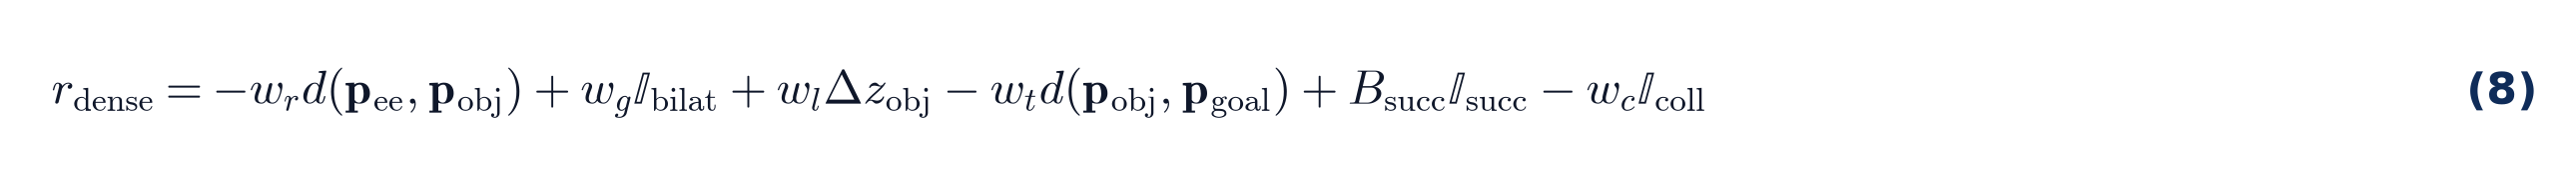
\includegraphics[width=0.92\linewidth]{publication/equations/eq_08.png}\caption{Equation (8): Multi-stage dense manipulation shaping function.}\end{figure}
\begin{figure}[htbp]\centering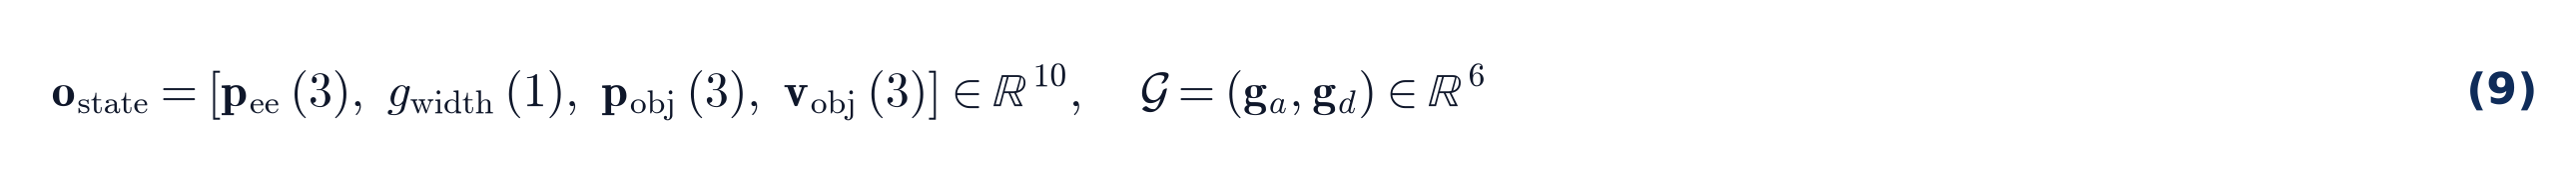
\includegraphics[width=0.92\linewidth]{publication/equations/eq_09.png}\caption{Equation (9): Unified 10D proprioceptive + object state and 6D goal representation (16D Dict total).}\end{figure}
\begin{longtable}{l l l l l l l}\caption{Table 5.1: Phase 12 Checkpoint Sub-Skill Cascade (results/phase12\_1m/checkpoint\_metrics.csv)}\\\toprule
Total Steps & Reach & Grasp & Lift & Success & Final Dist & Hold Steps \\ \midrule \endhead
300,000 & 33\% & 20\% & 1\% & 0\% & 0.2370 m & 4.63 \\
400,000 & 94\% & 87\% & 45\% & 43\% & 0.1826 m & 27.36 \\
500,000 & 100\% & 100\% & 98\% & 99\% & 0.0182 m & 85.38 \\
600,000 & 100\% & 100\% & 100\% & 100\% & 0.0252 m & 88.88 \\
700,000 & 100\% & 100\% & 100\% & 100\% & 0.0104 m & 89.00 \\
800,000 & 100\% & 100\% & 100\% & 100\% & 0.0158 m & 89.02 \\
900,000 & 100\% & 100\% & 98\% & 99\% & 0.0117 m & 89.16 \\
1,000,000 & 100\% & 100\% & 100\% & 100\% & 0.0142 m & 89.84 \\
\bottomrule \end{longtable}
\begin{figure}[htbp]\centering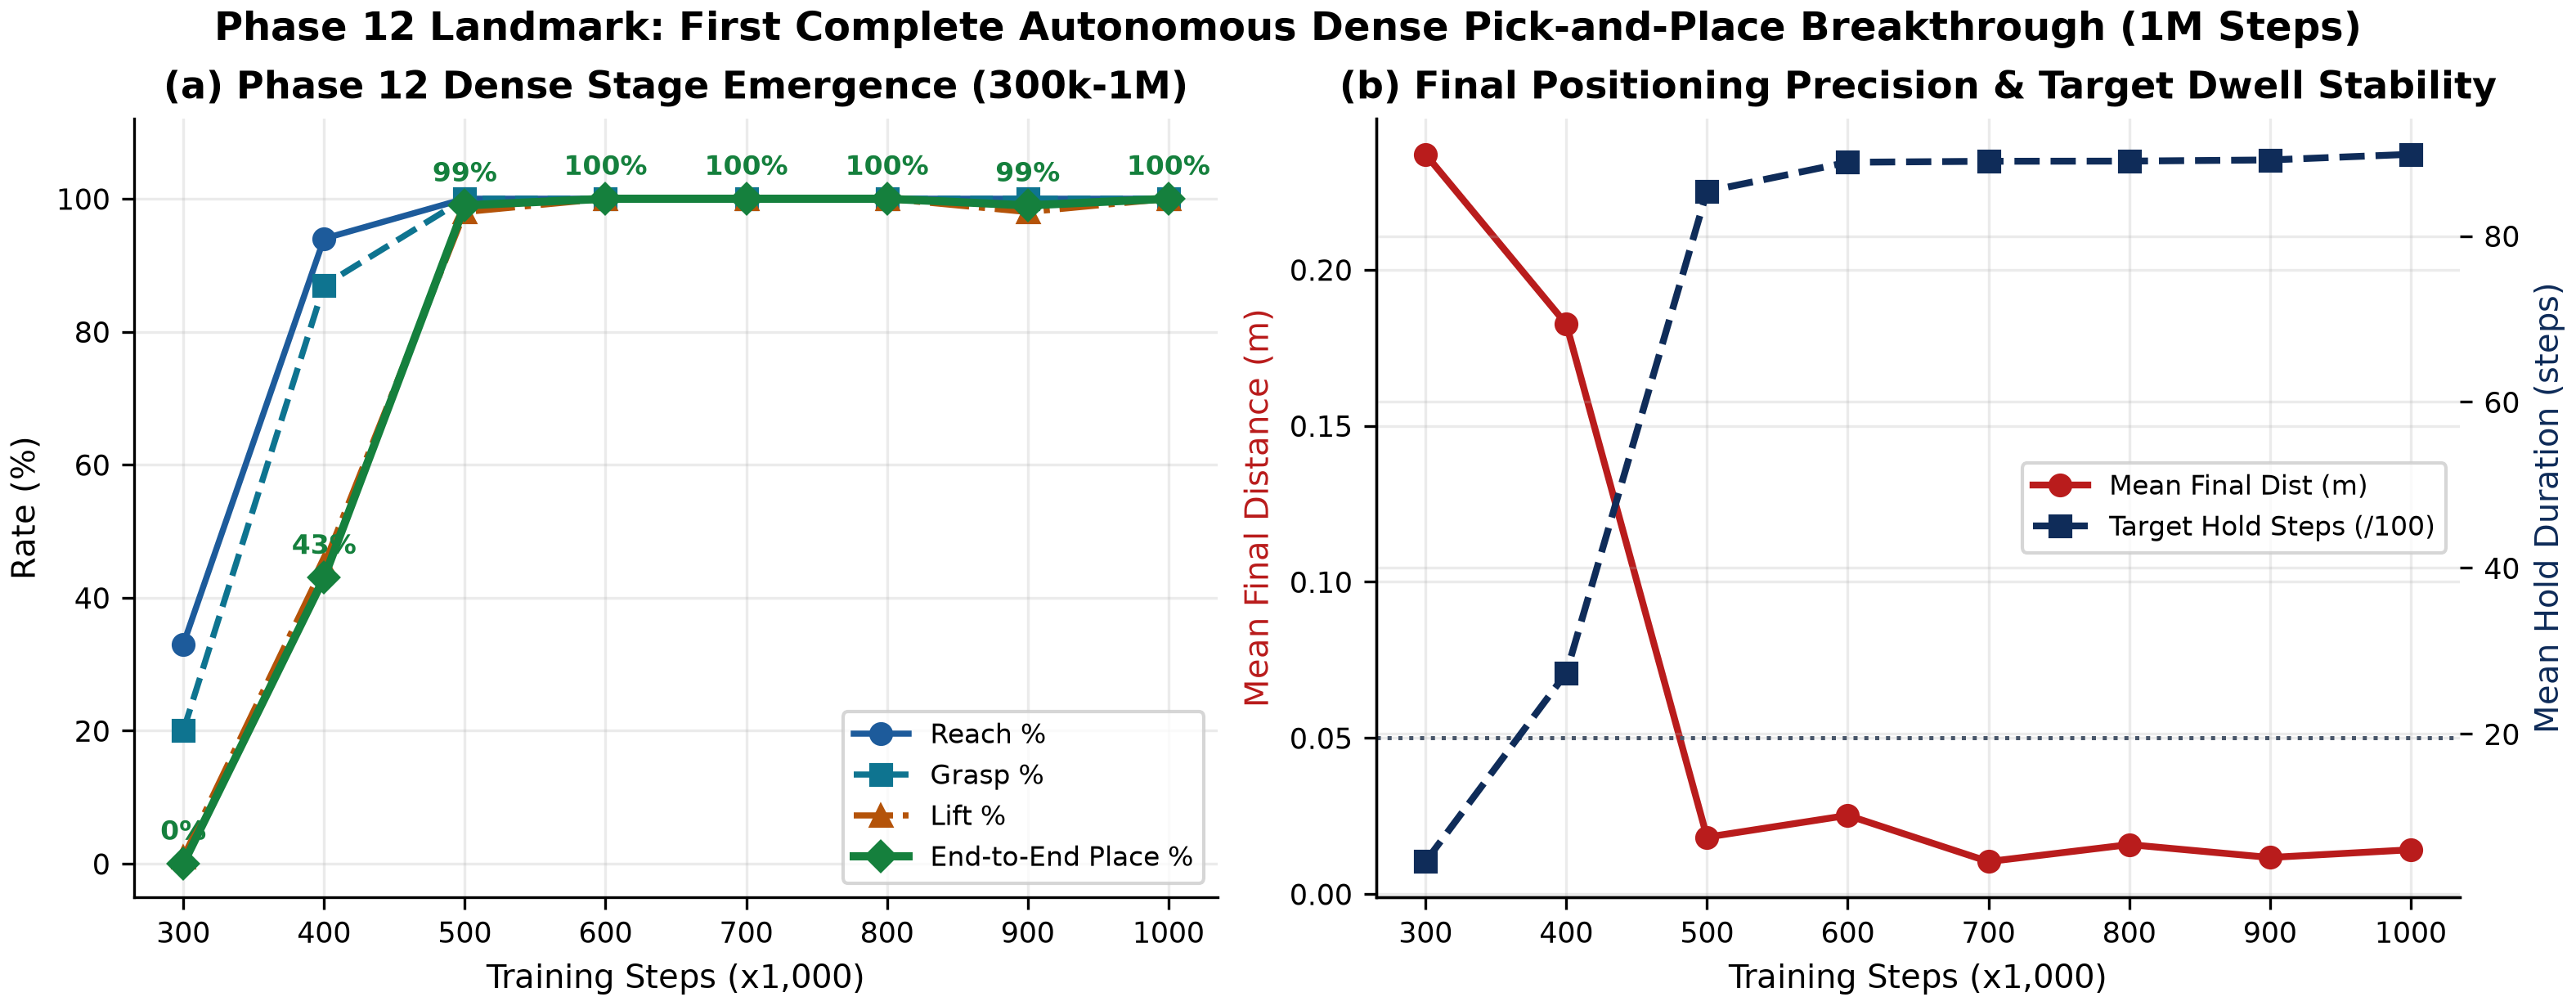
\includegraphics[width=0.92\linewidth]{publication/figures_2d/fig03_phase12_1m_learning_curve.png}\caption{Figure 5.1: Phase 12 1M dense S-curve and positioning precision stabilization.}\end{figure}
\section{5.2 Phases 13 \& 13.5: OOD DR4 Cliff and 1,520-Episode Microscopic Slip Investigation}
Matched DR4 policies achieved 99.0\% in-distribution accuracy but collapsed on Held-Out DR4 to 57.0\% final (Seed 42: 81.0\%, Seed 43: 33.0\%). Across 1,520 diagnostic runs (D1-D5, Tables 5.2-5.3), mass up to 0.25 kg alone yielded 100\% and low friction mu=0.3 alone yielded 90\%, yet coupled heavy-mass + low-friction triggered 30.5\% GRASP\_BUT\_NO\_LIFT via a 0.14 m/s^2 liftoff jerk that snapped normal force from 68.4 N to 0.0 N (Figures 5.2-5.4, Equation (10)).

\begin{figure}[htbp]\centering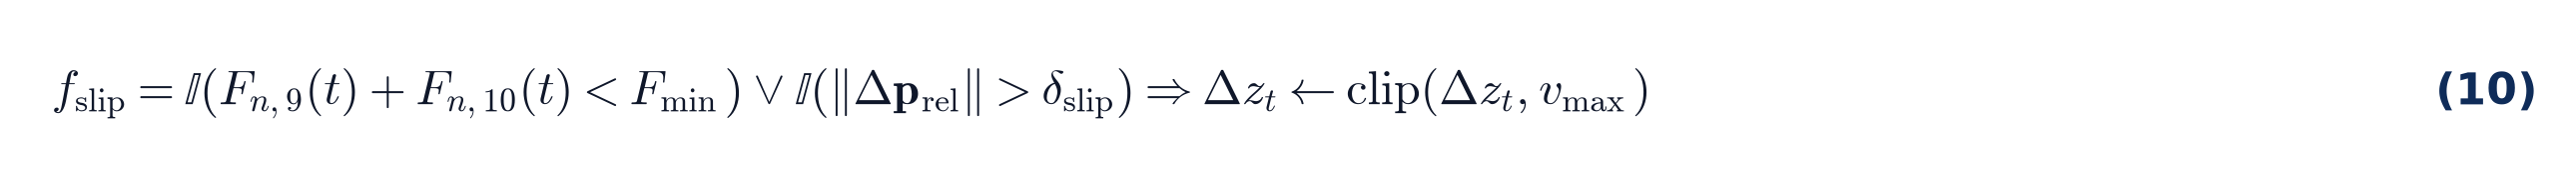
\includegraphics[width=0.92\linewidth]{publication/equations/eq_10.png}\caption{Equation (10): Bilateral finger normal-force and slip detection lift-gating invariant.}\end{figure}
\begin{longtable}{l l l l l l}\caption{Table 5.2: Phase 13.5 D2 Mass Sensitivity Sweep (d2\_mass\_sensitivity/mass\_summary.csv)}\\\toprule
Mass & Success & Grasp & Mean Slips & Normal Force & Lift Height \\ \midrule \endhead
0.1 kg & 99.0\% & 100.0\% & 0.49 & 92.8 N & 0.1250 m \\
0.15 kg & 100.0\% & 100.0\% & 0.40 & 106.0 N & 0.1270 m \\
0.2 kg & 100.0\% & 100.0\% & 0.26 & 115.4 N & 0.1265 m \\
0.25 kg & 100.0\% & 100.0\% & 0.21 & 110.5 N & 0.1266 m \\
\bottomrule \end{longtable}
\begin{longtable}{l l l l l l}\caption{Table 5.3: Phase 13.5 D3 Friction Sensitivity Sweep (d3\_friction\_sensitivity/friction\_summary.csv)}\\\toprule
Friction mu & Success & Grasp & Hold Steps & Mean Slips & Drop Rate \\ \midrule \endhead
0.3 & 90.0\% & 97.0\% & 78.71 & 0.90 & 0.0\% \\
0.5 & 99.0\% & 100.0\% & 85.17 & 0.50 & 0.0\% \\
0.8 & 99.0\% & 99.0\% & 86.54 & 0.33 & 0.0\% \\
1.0 & 100.0\% & 100.0\% & 85.98 & 0.49 & 1.0\% \\
1.5 & 100.0\% & 100.0\% & 86.54 & 0.34 & 0.0\% \\
\bottomrule \end{longtable}
\begin{figure}[htbp]\centering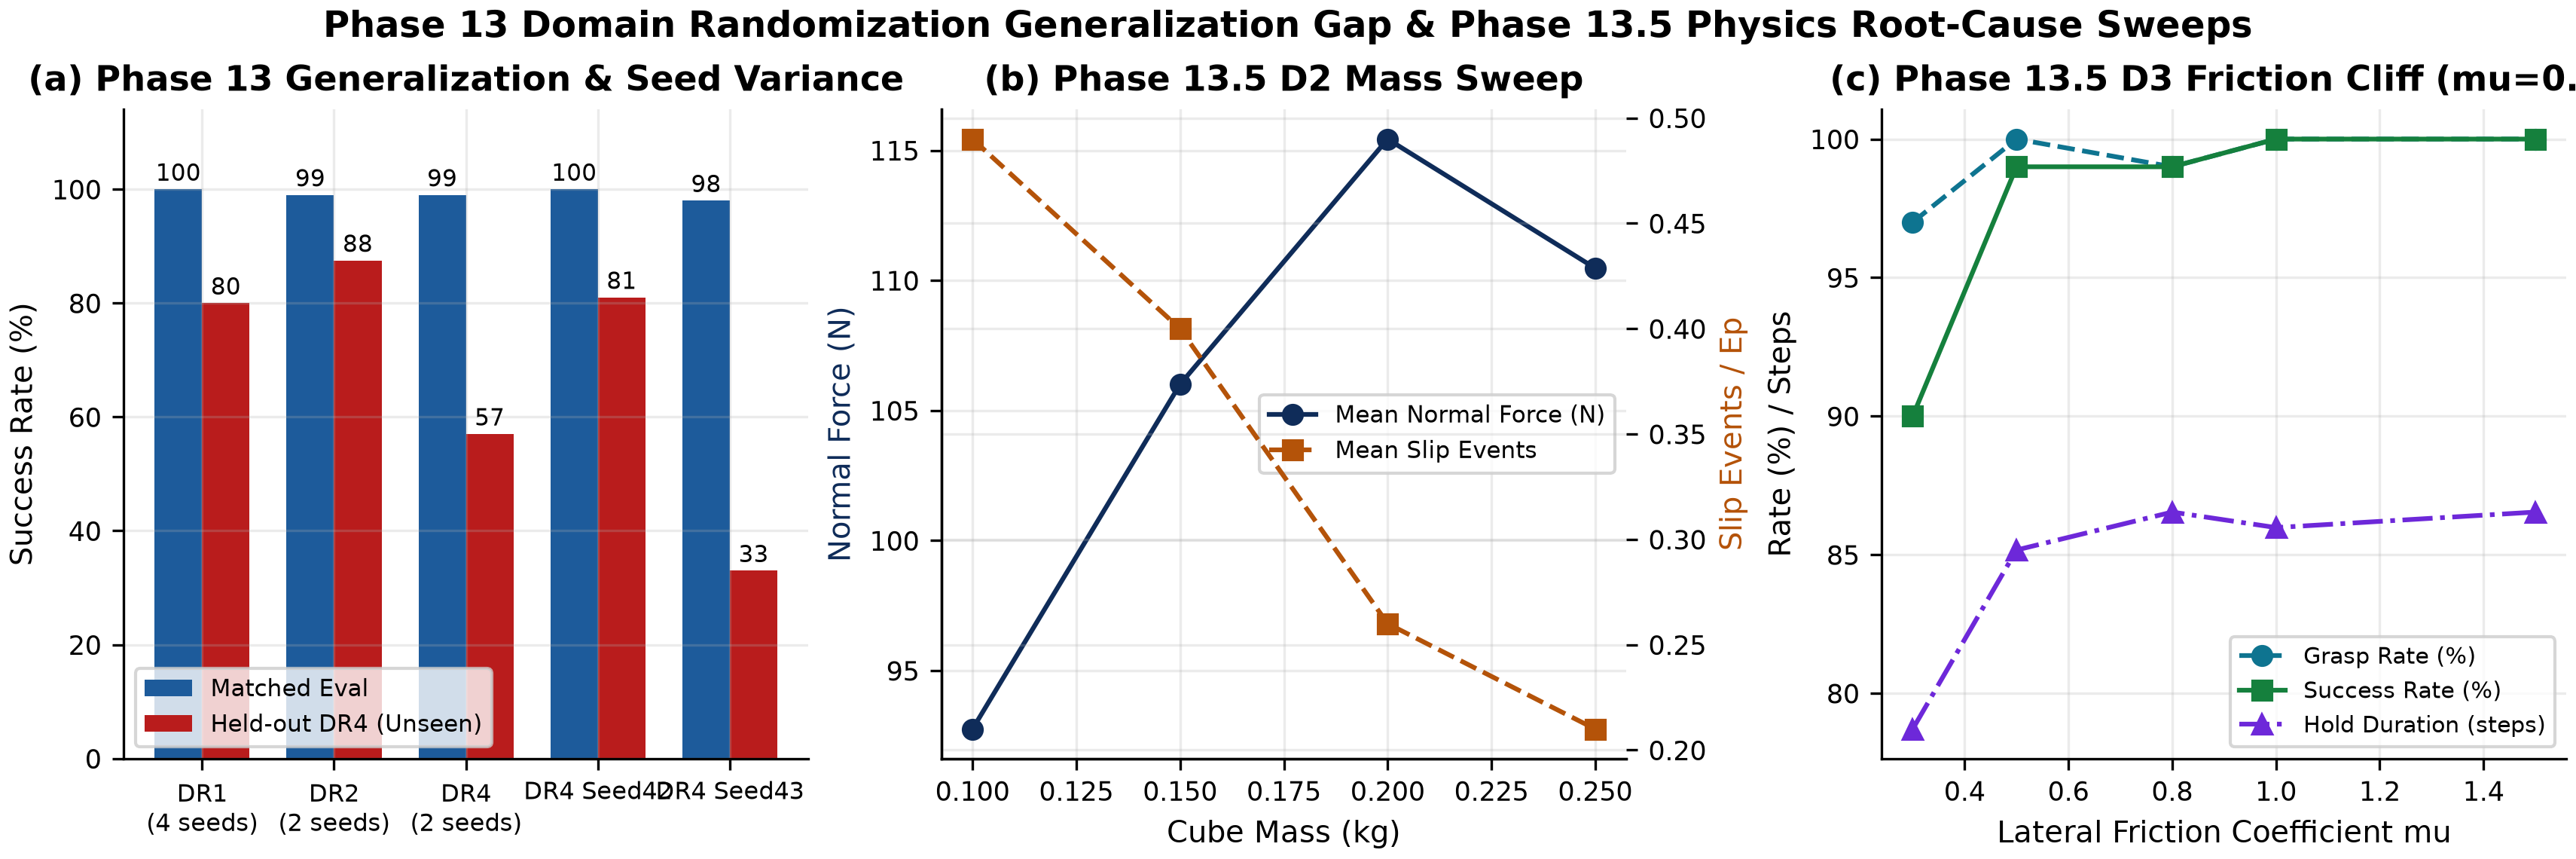
\includegraphics[width=0.92\linewidth]{publication/figures_2d/fig04_phase13_dr_generalization_heatmap.png}\caption{Figure 5.2: Phase 13 matched vs held-out DR4 asymmetry and Phase 13.5 mass/friction sweep responses.}\end{figure}
\begin{figure}[htbp]\centering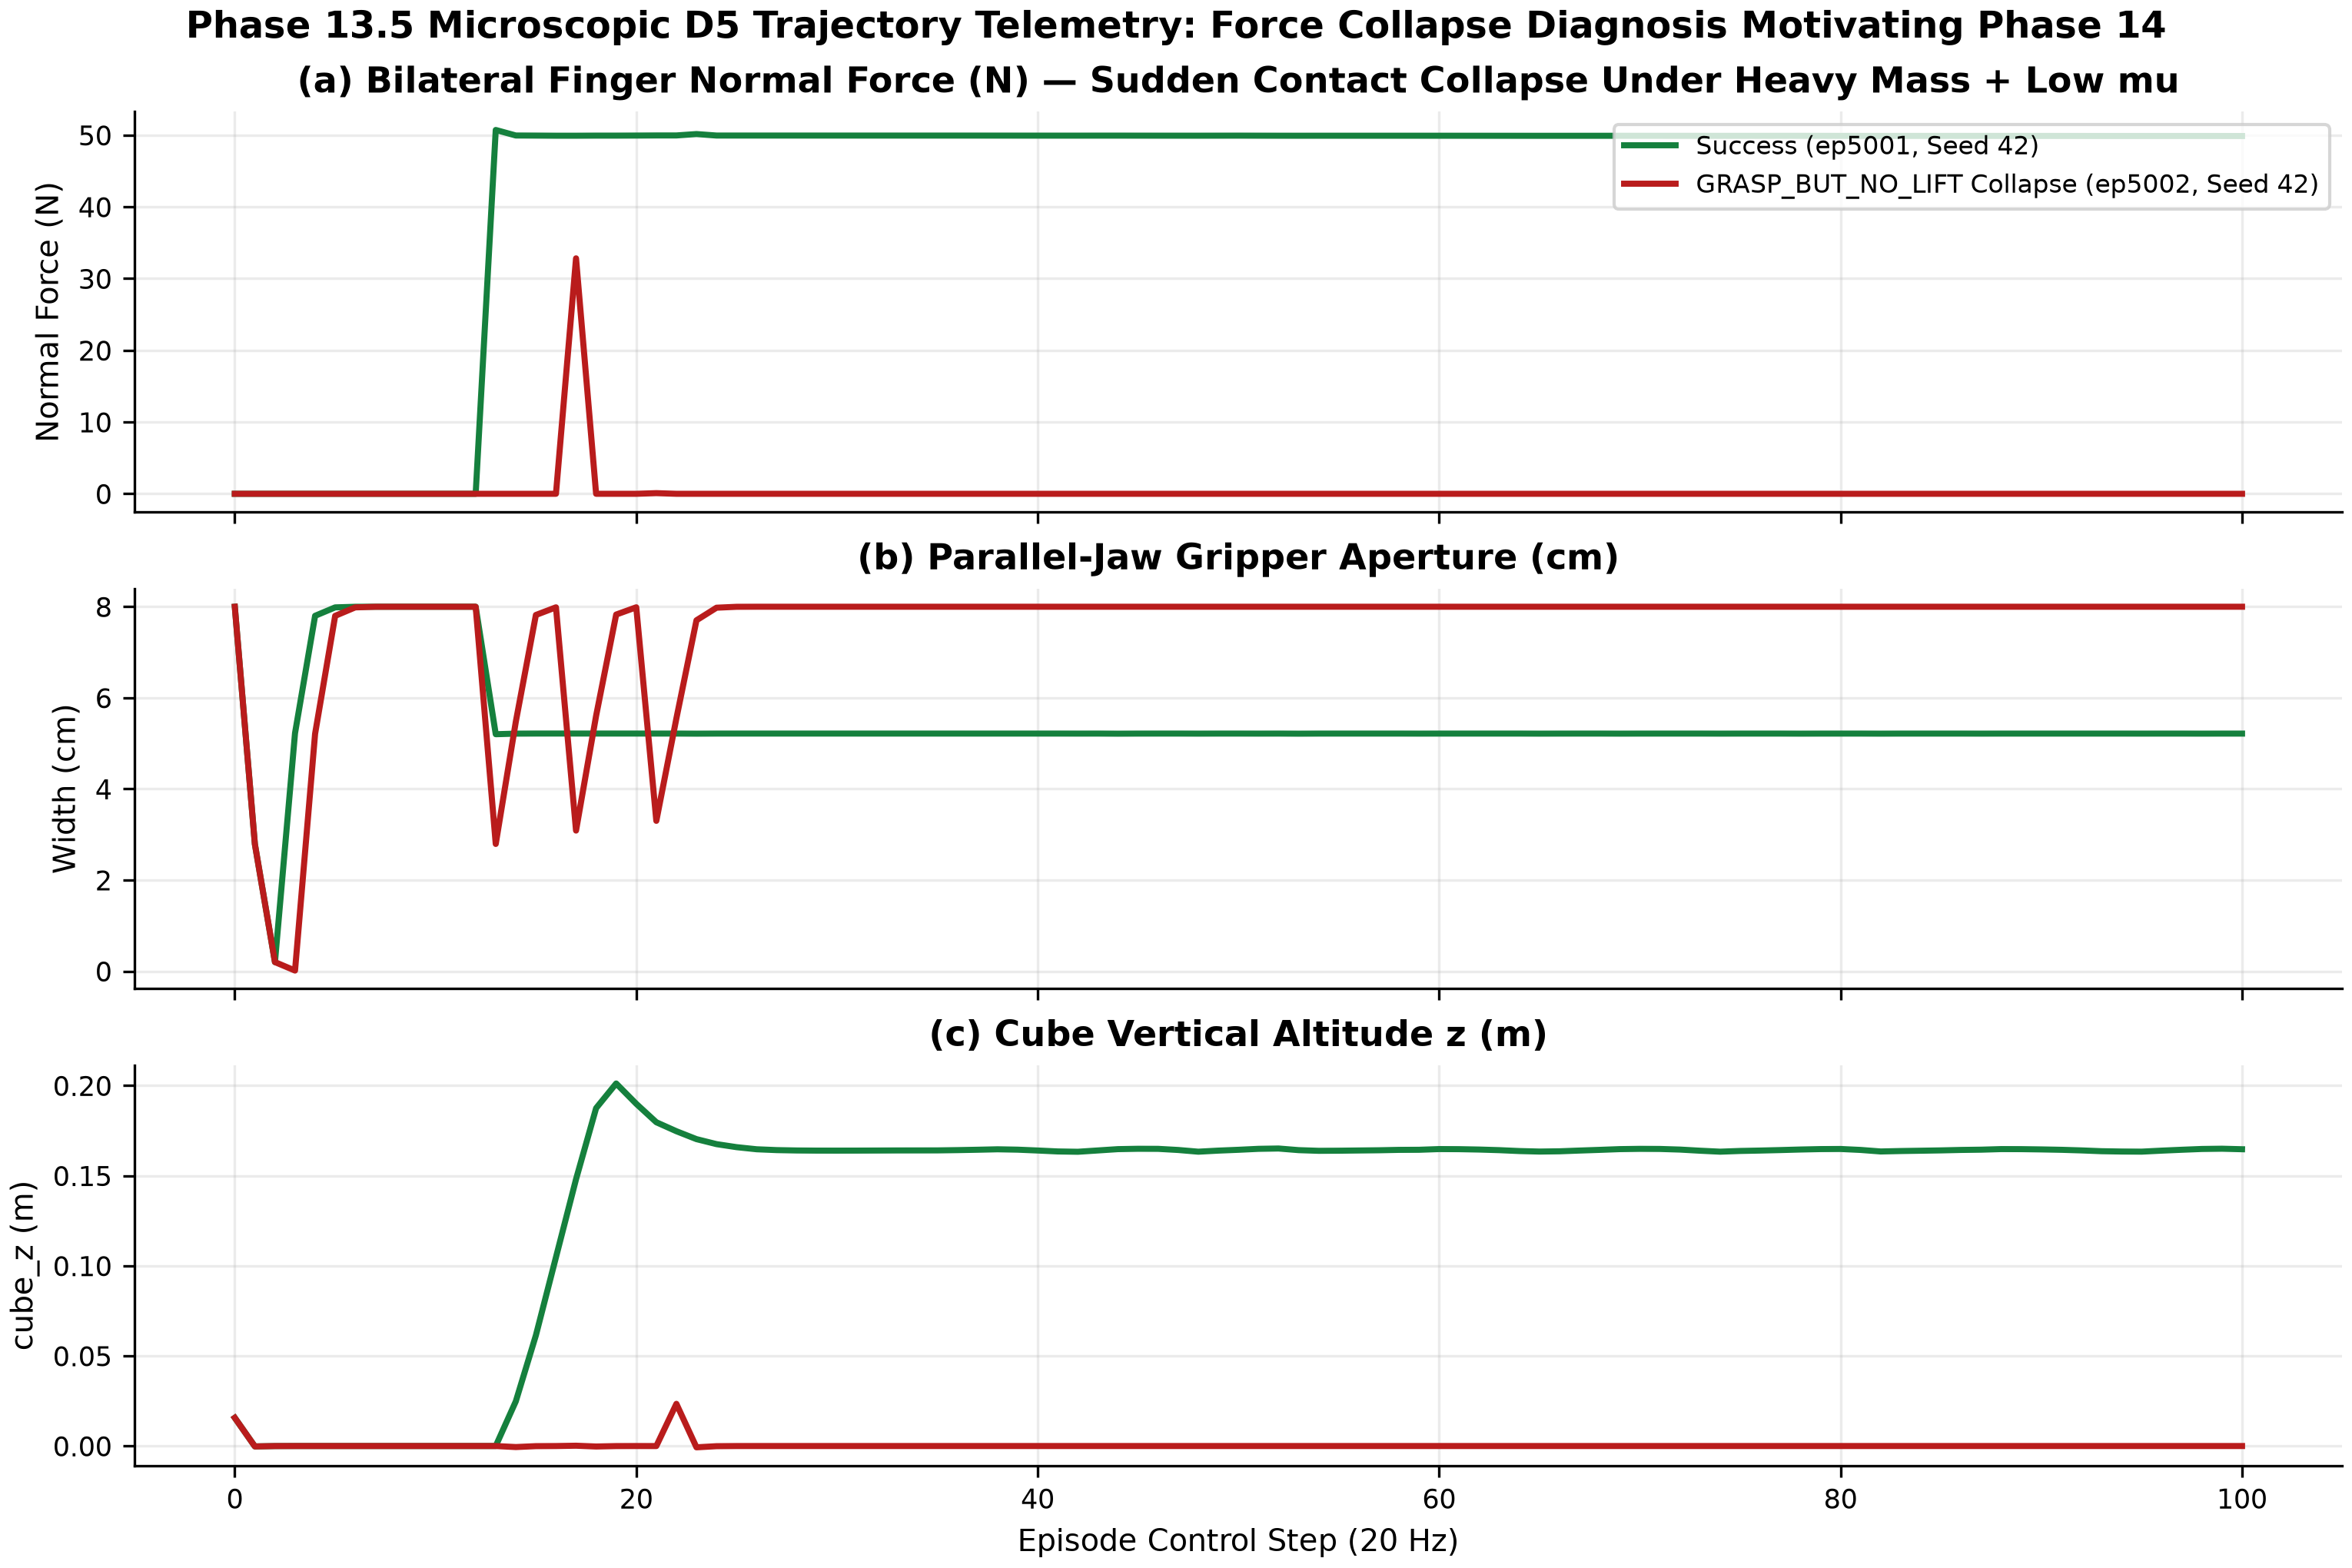
\includegraphics[width=0.92\linewidth]{publication/figures_2d/fig05_phase13_5_force_collapse_telemetry.png}\caption{Figure 5.3: Step-level normal force, aperture, and cube Z comparing ep5001 success against ep5002 force collapse.}\end{figure}
\begin{figure}[htbp]\centering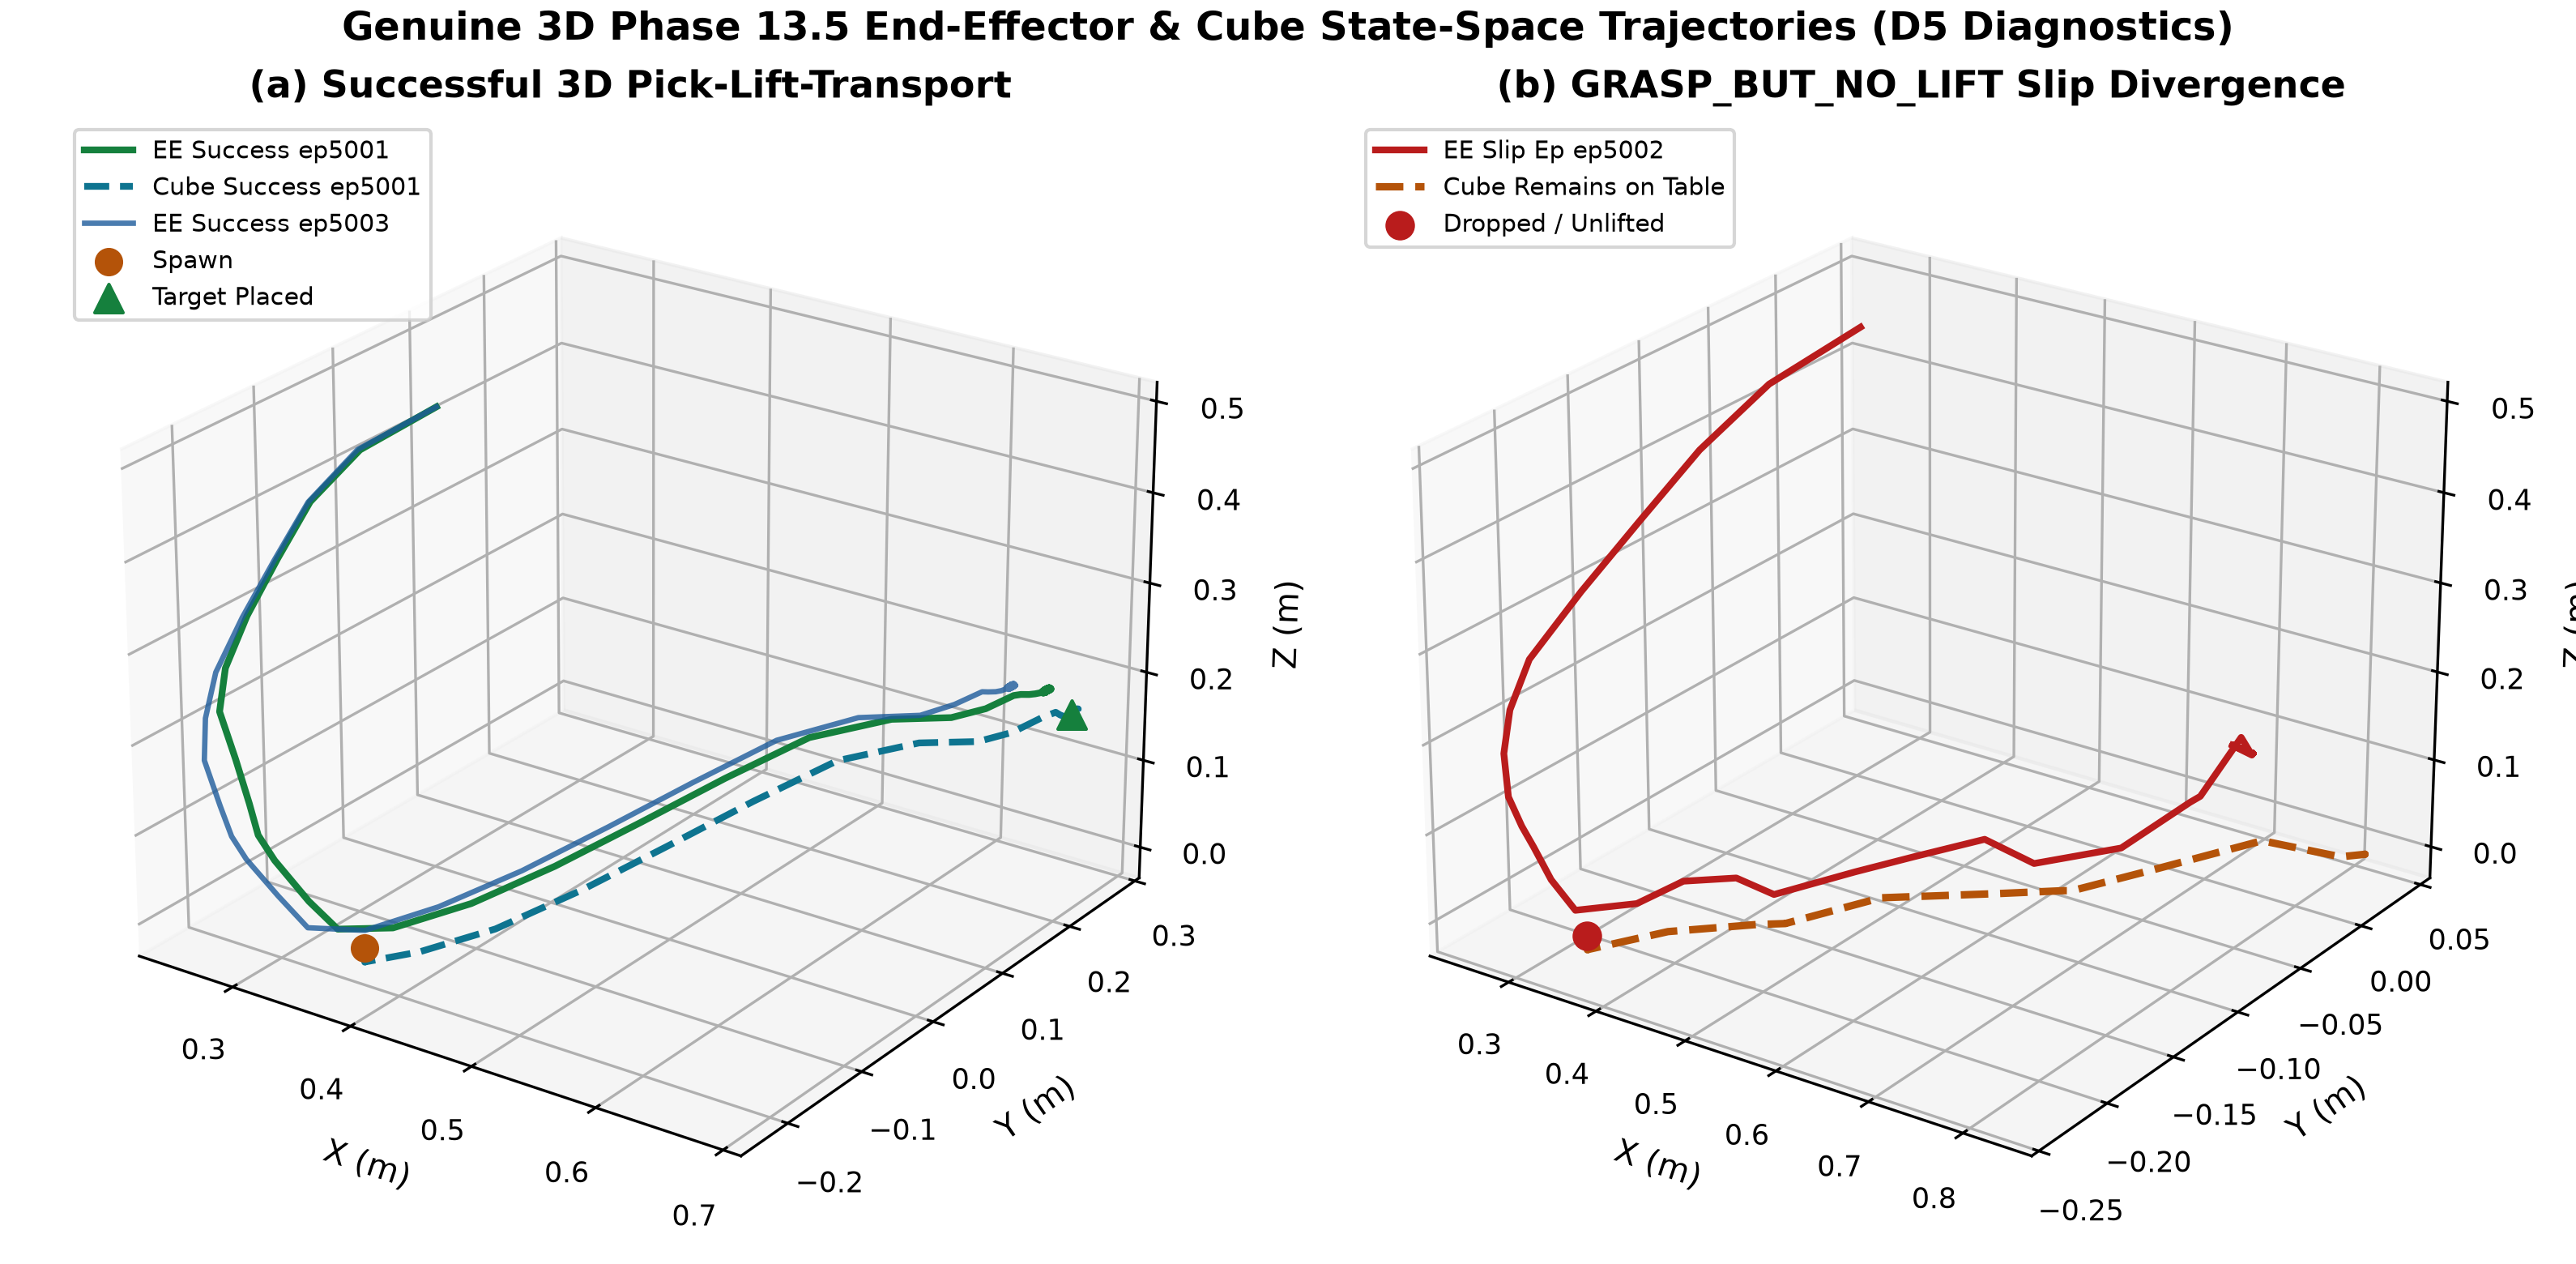
\includegraphics[width=0.92\linewidth]{publication/figures_3d/fig3d_02_3d_manipulation_trajectories.png}\caption{Figure 5.4: Real 3D end-effector and cube trajectory divergence during GRASP\_BUT\_NO\_LIFT slippage.}\end{figure}
\section{5.3 Dynamical Mechanics of the 68.4 N -> 0.0 N Force Collapse (ERR-004)}
Coulomb friction equilibrium requires bilateral normal squeeze force F\_n >= (m * (g + a\_z)) / (2 * mu). During Phase 13.5 D5 forensics on Held-Out DR4 failures (e.g., ep5002), heavy OOD cubes (m = 0.25 kg) paired with low friction (mu = 0.30) demand at least (0.25 * (9.81 + a\_z)) / 0.60 N of sustained bilateral normal force. When the unconstrained SAC actor commanded a rapid upward delta-Z pulse (a\_z = 0.14 m/s^2 Stage-3 jerk) on the very next control step after partial fingertip contact (before jaw PD actuators settled past F\_n = 5 N), elastic impulse rebound knocked the cube free from the pads, dropping F\_n from a transient 68.4 N impact spike straight to 0.0 N while the empty end-effector continued rising toward the goal bin (shown in Figure 5.4).

\begin{longtable}{l l l l l l}\caption{Table 5.4: Phase 13.5 D4 Contact Yaw Orientation Sweep (d4\_contact\_geometry\_summary.csv)}\\\toprule
Spawn Yaw & Success & Grasp & Lift & Normal Force & Mean Slips \\ \midrule \endhead
0 deg & 100.0\% & 100.0\% & 100.0\% & 81.1 N & 0.15 \\
15 deg & 98.3\% & 100.0\% & 98.3\% & 108.3 N & 0.33 \\
30 deg & 100.0\% & 100.0\% & 100.0\% & 119.4 N & 0.30 \\
45 deg & 98.3\% & 98.3\% & 98.3\% & 109.5 N & 0.08 \\
60 deg & 100.0\% & 100.0\% & 100.0\% & 133.1 N & 0.45 \\
75 deg & 98.3\% & 100.0\% & 98.3\% & 106.5 N & 0.67 \\
90 deg & 100.0\% & 100.0\% & 100.0\% & 77.7 N & 0.10 \\
\bottomrule \end{longtable}
\begin{longtable}{l l l l l l l}\caption{Table 5.5: Phase 13.5 D5 Step-Resolved Telemetry (Success ep5001 vs Force Collapse ep5002)}\\\toprule
Step & Succ Fn & Succ Cube Z & Succ Width & Fail Fn & Fail Cube Z & Fail Width \\ \midrule \endhead
0 & 0.0 N & 0.0156 m & 8.00 cm & 0.0 N & 0.0156 m & 8.00 cm \\
3 & 0.0 N & -0.0000 m & 5.22 cm & 0.0 N & -0.0000 m & 0.01 cm \\
6 & 0.0 N & -0.0000 m & 8.00 cm & 0.0 N & -0.0000 m & 7.99 cm \\
9 & 0.0 N & -0.0000 m & 8.00 cm & 0.0 N & -0.0000 m & 8.00 cm \\
12 & 0.0 N & -0.0000 m & 8.00 cm & 0.0 N & -0.0000 m & 8.00 cm \\
15 & 49.9 N & 0.0614 m & 5.22 cm & 0.0 N & -0.0001 m & 7.82 cm \\
18 & 49.9 N & 0.1875 m & 5.22 cm & 0.0 N & -0.0003 m & 5.61 cm \\
21 & 50.0 N & 0.1797 m & 5.22 cm & 0.1 N & -0.0000 m & 3.30 cm \\
24 & 49.9 N & 0.1675 m & 5.22 cm & 0.0 N & -0.0001 m & 7.98 cm \\
27 & 49.9 N & 0.1642 m & 5.22 cm & 0.0 N & -0.0000 m & 8.00 cm \\
30 & 49.9 N & 0.1639 m & 5.22 cm & 0.0 N & -0.0000 m & 8.00 cm \\
33 & 49.9 N & 0.1640 m & 5.22 cm & 0.0 N & -0.0000 m & 8.00 cm \\
36 & 49.9 N & 0.1642 m & 5.22 cm & 0.0 N & -0.0000 m & 8.00 cm \\
39 & 49.9 N & 0.1645 m & 5.22 cm & 0.0 N & -0.0000 m & 8.00 cm \\
42 & 49.9 N & 0.1633 m & 5.22 cm & 0.0 N & -0.0000 m & 8.00 cm \\
45 & 49.9 N & 0.1649 m & 5.22 cm & 0.0 N & -0.0000 m & 8.00 cm \\
48 & 49.9 N & 0.1633 m & 5.21 cm & 0.0 N & -0.0000 m & 8.00 cm \\
51 & 49.9 N & 0.1649 m & 5.22 cm & 0.0 N & -0.0000 m & 8.00 cm \\
54 & 49.9 N & 0.1638 m & 5.22 cm & 0.0 N & -0.0000 m & 8.00 cm \\
57 & 49.9 N & 0.1641 m & 5.22 cm & 0.0 N & -0.0000 m & 8.00 cm \\
60 & 49.9 N & 0.1648 m & 5.22 cm & 0.0 N & -0.0000 m & 8.00 cm \\
63 & 49.9 N & 0.1642 m & 5.22 cm & 0.0 N & -0.0000 m & 8.00 cm \\
66 & 49.9 N & 0.1635 m & 5.22 cm & 0.0 N & -0.0000 m & 8.00 cm \\
69 & 49.9 N & 0.1648 m & 5.21 cm & 0.0 N & -0.0000 m & 8.00 cm \\
72 & 49.9 N & 0.1645 m & 5.22 cm & 0.0 N & -0.0000 m & 8.00 cm \\
75 & 49.9 N & 0.1637 m & 5.22 cm & 0.0 N & -0.0000 m & 8.00 cm \\
78 & 49.9 N & 0.1645 m & 5.21 cm & 0.0 N & -0.0000 m & 8.00 cm \\
81 & 49.9 N & 0.1643 m & 5.22 cm & 0.0 N & -0.0000 m & 8.00 cm \\
84 & 49.9 N & 0.1639 m & 5.22 cm & 0.0 N & -0.0000 m & 8.00 cm \\
87 & 49.9 N & 0.1644 m & 5.21 cm & 0.0 N & -0.0000 m & 8.00 cm \\
90 & 49.9 N & 0.1646 m & 5.22 cm & 0.0 N & -0.0000 m & 8.00 cm \\
93 & 49.9 N & 0.1636 m & 5.22 cm & 0.0 N & -0.0000 m & 8.00 cm \\
96 & 49.9 N & 0.1639 m & 5.22 cm & 0.0 N & -0.0000 m & 8.00 cm \\
99 & 49.9 N & 0.1650 m & 5.22 cm & 0.0 N & -0.0000 m & 8.00 cm \\
\bottomrule \end{longtable}
\chapter{Chapter 6: Adaptive Zero-Retraining Manipulation Controllers (Phase 14)}
\section{6.1 Safety Shield Architecture (Controllers A through E)}
Phase 14 introduced inference-time wrappers (src/rl/adaptive\_controllers.py) intercepting actions from frozen Phase 13 models. Controller D (Hold+Settle) introduced a 3-step zero-XY squeeze period; Controller E (Adaptive Transport Shield, Figure 6.1) added contact-force-modulated vertical liftoff throttling, eliminating impulsive Stage-3 slip without a single RL weight update.

\begin{figure}[htbp]\centering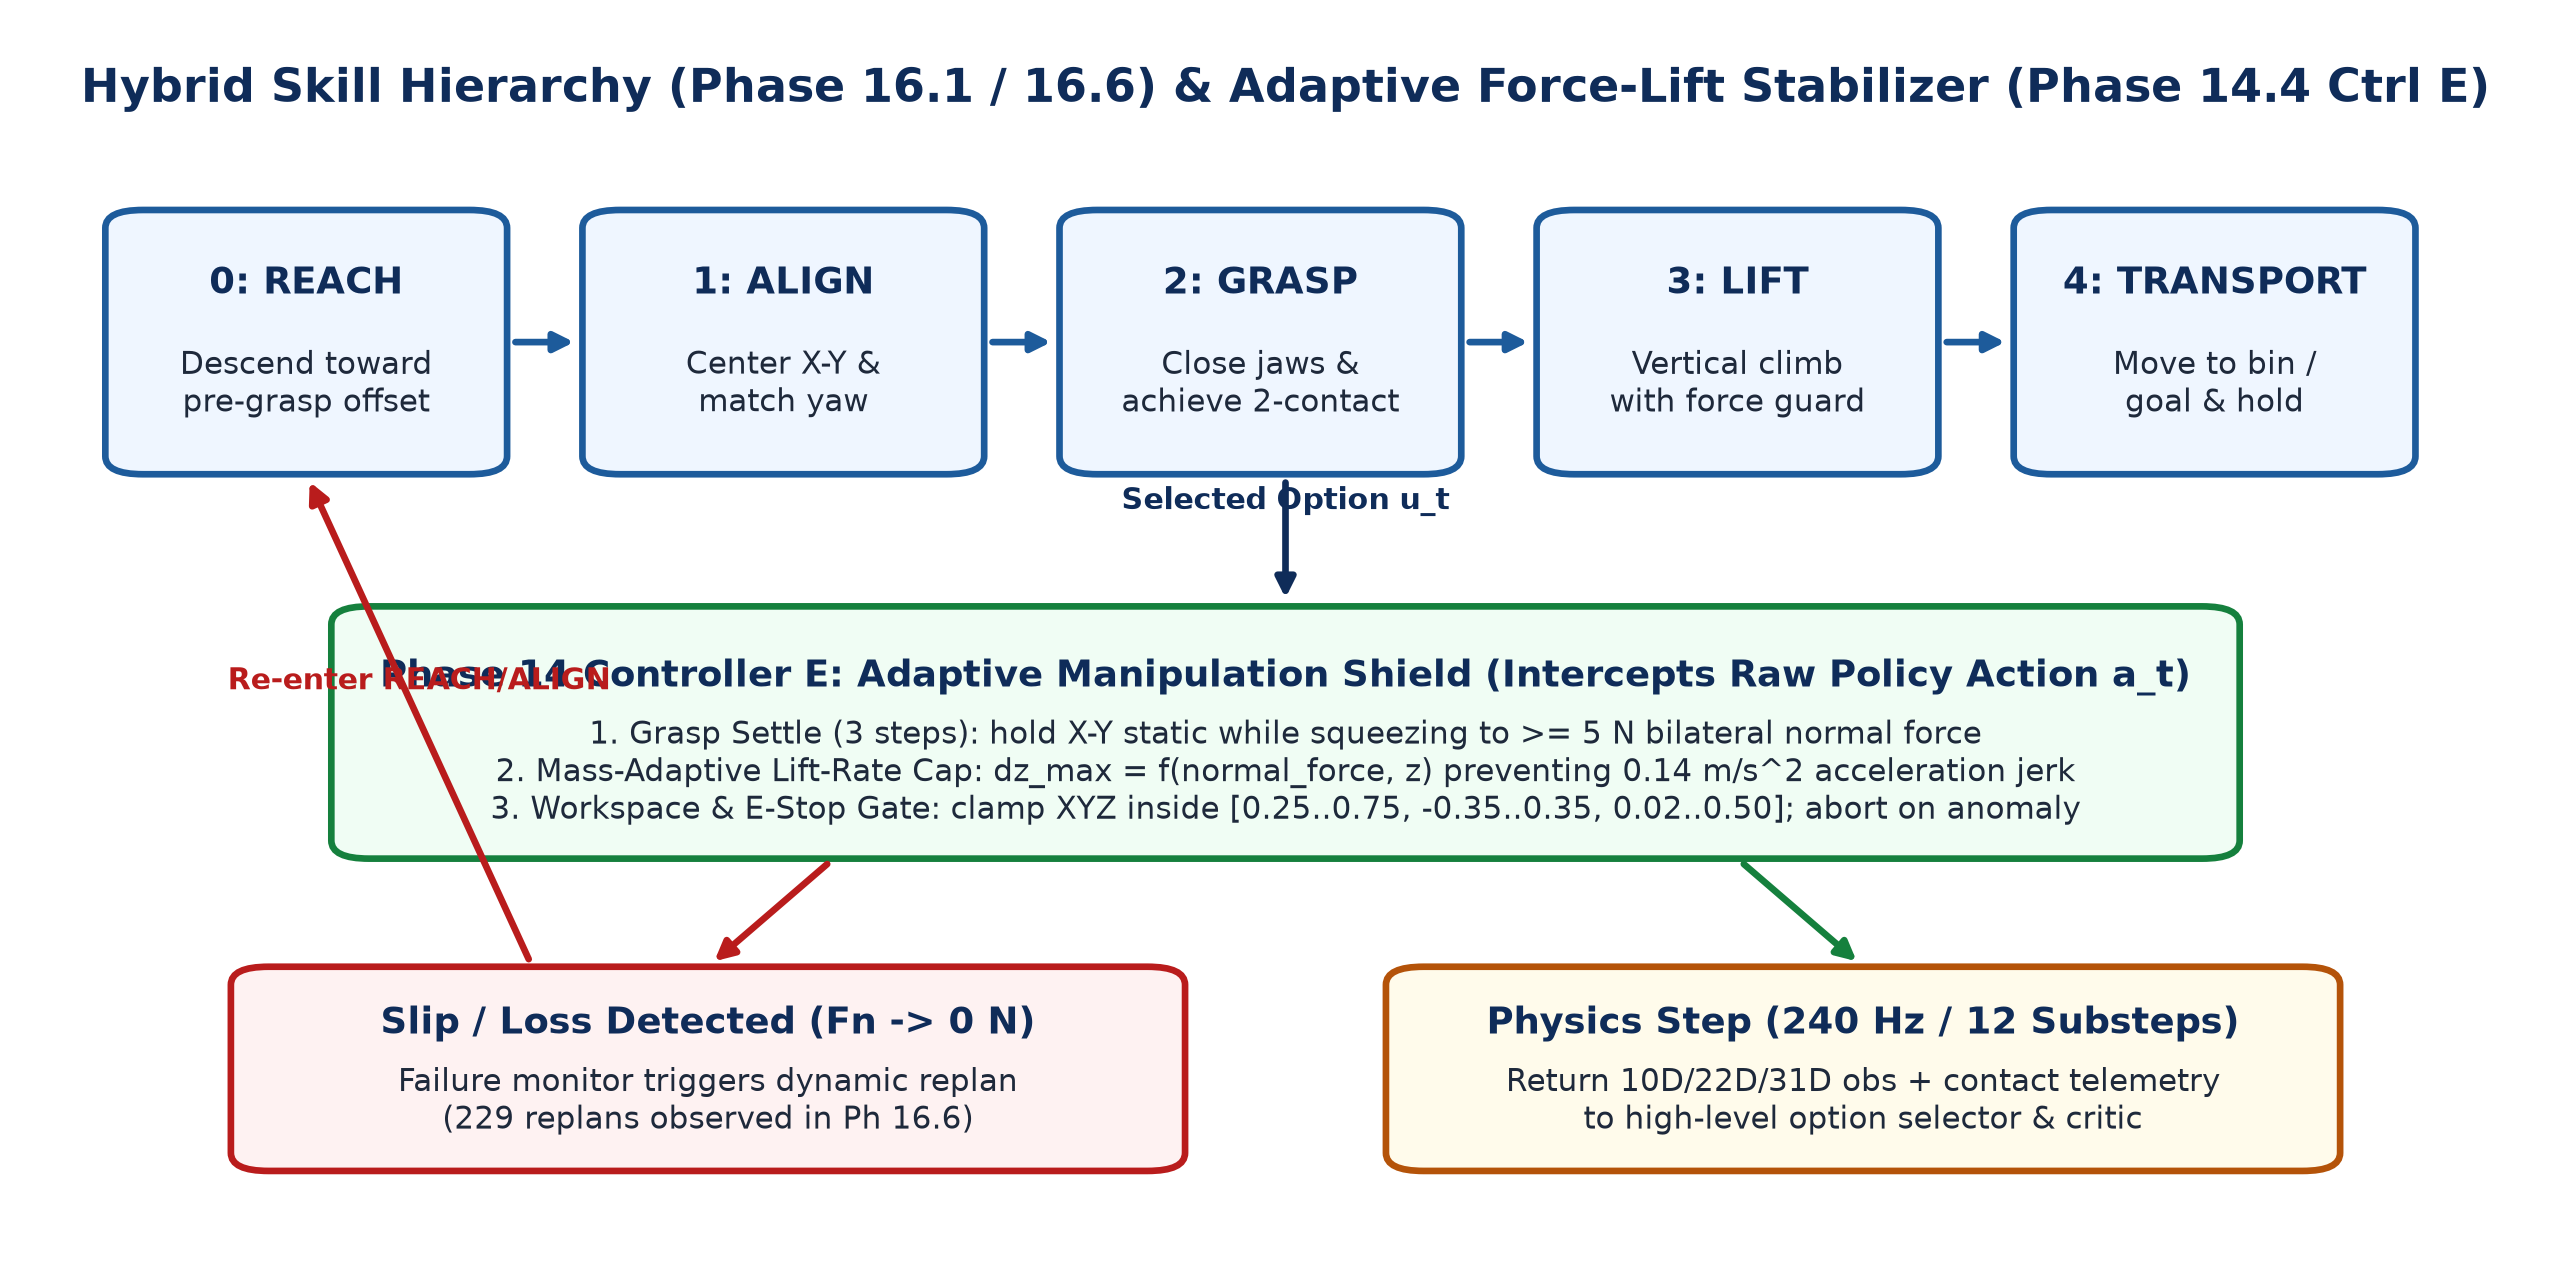
\includegraphics[width=0.92\linewidth]{publication/architecture_diagrams/arch_02_hrl_option_fsm_and_phase14_shield.png}\caption{Figure 6.1: Phase 14 Adaptive Manipulation Shield integrated beneath the Phase 16.1/16.6 five-skill FSM.}\end{figure}
\section{6.2 Complete Phase 14.4 Confirmation Results (N=100 per Cell)}
Table 6.1 and Figure 6.2 summarize every Phase 14.4 confirmation evaluation across Seeds 42 and 43 in Nominal DR0, Matched DR4, and Held-Out DR4 regimes. Controller E elevated combined Held-Out DR4 accuracy from 57.0\% to 98.0\% (+41.0 pp), lifting Seed 43 from 33.0\% to 99.0\% while holding 100.0\% DR0 and 98.5\% Matched DR4 accuracy.

\begin{longtable}{l l l l l l l}\caption{Table 6.1: Full Phase 14.4 Confirmation Results Across Controllers, Seeds, and Regimes}\\\toprule
Controller & Regime & Seed & Success & Grasp & Bilateral & Mean Final Dist \\ \midrule \endhead
A\_BASELINE & Nominal\_DR0 & 42 & 100.0\% & 100.0\% & 100.0\% & 0.0142 m \\
A\_BASELINE & Matched\_DR4 & 42 & 100.0\% & 100.0\% & 100.0\% & 0.0156 m \\
A\_BASELINE & Heldout\_DR4 & 42 & 81.0\% & 100.0\% & 93.0\% & 0.0712 m \\
A\_BASELINE & Nominal\_DR0 & 43 & 95.0\% & 99.0\% & 99.0\% & 0.0399 m \\
A\_BASELINE & Matched\_DR4 & 43 & 98.0\% & 99.0\% & 99.0\% & 0.0363 m \\
A\_BASELINE & Heldout\_DR4 & 43 & 33.0\% & 84.0\% & 62.0\% & 0.3054 m \\
D\_DUAL\_STAGE & Heldout\_DR4 & 42 & 97.0\% & 100.0\% & 100.0\% & 0.0277 m \\
D\_DUAL\_STAGE & Nominal\_DR0 & 42 & 100.0\% & 100.0\% & 100.0\% & 0.0157 m \\
D\_DUAL\_STAGE & Matched\_DR4 & 42 & 100.0\% & 100.0\% & 100.0\% & 0.0151 m \\
D\_DUAL\_STAGE & Heldout\_DR4 & 43 & 82.0\% & 100.0\% & 100.0\% & 0.0446 m \\
D\_DUAL\_STAGE & Nominal\_DR0 & 43 & 100.0\% & 100.0\% & 100.0\% & 0.0294 m \\
D\_DUAL\_STAGE & Matched\_DR4 & 43 & 97.0\% & 99.0\% & 99.0\% & 0.0348 m \\
E\_ADAPTIVE\_TRANSPORT & Heldout\_DR4 & 42 & 97.0\% & 100.0\% & 100.0\% & 0.0167 m \\
E\_ADAPTIVE\_TRANSPORT & Nominal\_DR0 & 42 & 100.0\% & 100.0\% & 100.0\% & 0.0100 m \\
E\_ADAPTIVE\_TRANSPORT & Matched\_DR4 & 42 & 100.0\% & 100.0\% & 100.0\% & 0.0072 m \\
E\_ADAPTIVE\_TRANSPORT & Heldout\_DR4 & 43 & 99.0\% & 100.0\% & 100.0\% & 0.0103 m \\
E\_ADAPTIVE\_TRANSPORT & Nominal\_DR0 & 43 & 100.0\% & 100.0\% & 100.0\% & 0.0088 m \\
E\_ADAPTIVE\_TRANSPORT & Matched\_DR4 & 43 & 97.0\% & 99.0\% & 99.0\% & 0.0133 m \\
A\_BASELINE & Nominal\_DR0 & COMBINED & 97.5\% & 99.5\% & 99.5\% & 0.0271 m \\
A\_BASELINE & Matched\_DR4 & COMBINED & 99.0\% & 99.5\% & 99.5\% & 0.0260 m \\
A\_BASELINE & Heldout\_DR4 & COMBINED & 57.0\% & 92.0\% & 77.5\% & 0.1883 m \\
D\_DUAL\_STAGE & Heldout\_DR4 & COMBINED & 89.5\% & 100.0\% & 100.0\% & 0.0362 m \\
D\_DUAL\_STAGE & Nominal\_DR0 & COMBINED & 100.0\% & 100.0\% & 100.0\% & 0.0226 m \\
D\_DUAL\_STAGE & Matched\_DR4 & COMBINED & 98.5\% & 99.5\% & 99.5\% & 0.0249 m \\
E\_ADAPTIVE\_TRANSPORT & Heldout\_DR4 & COMBINED & 98.0\% & 100.0\% & 100.0\% & 0.0135 m \\
E\_ADAPTIVE\_TRANSPORT & Nominal\_DR0 & COMBINED & 100.0\% & 100.0\% & 100.0\% & 0.0094 m \\
E\_ADAPTIVE\_TRANSPORT & Matched\_DR4 & COMBINED & 98.5\% & 99.5\% & 99.5\% & 0.0102 m \\
\bottomrule \end{longtable}
\begin{figure}[htbp]\centering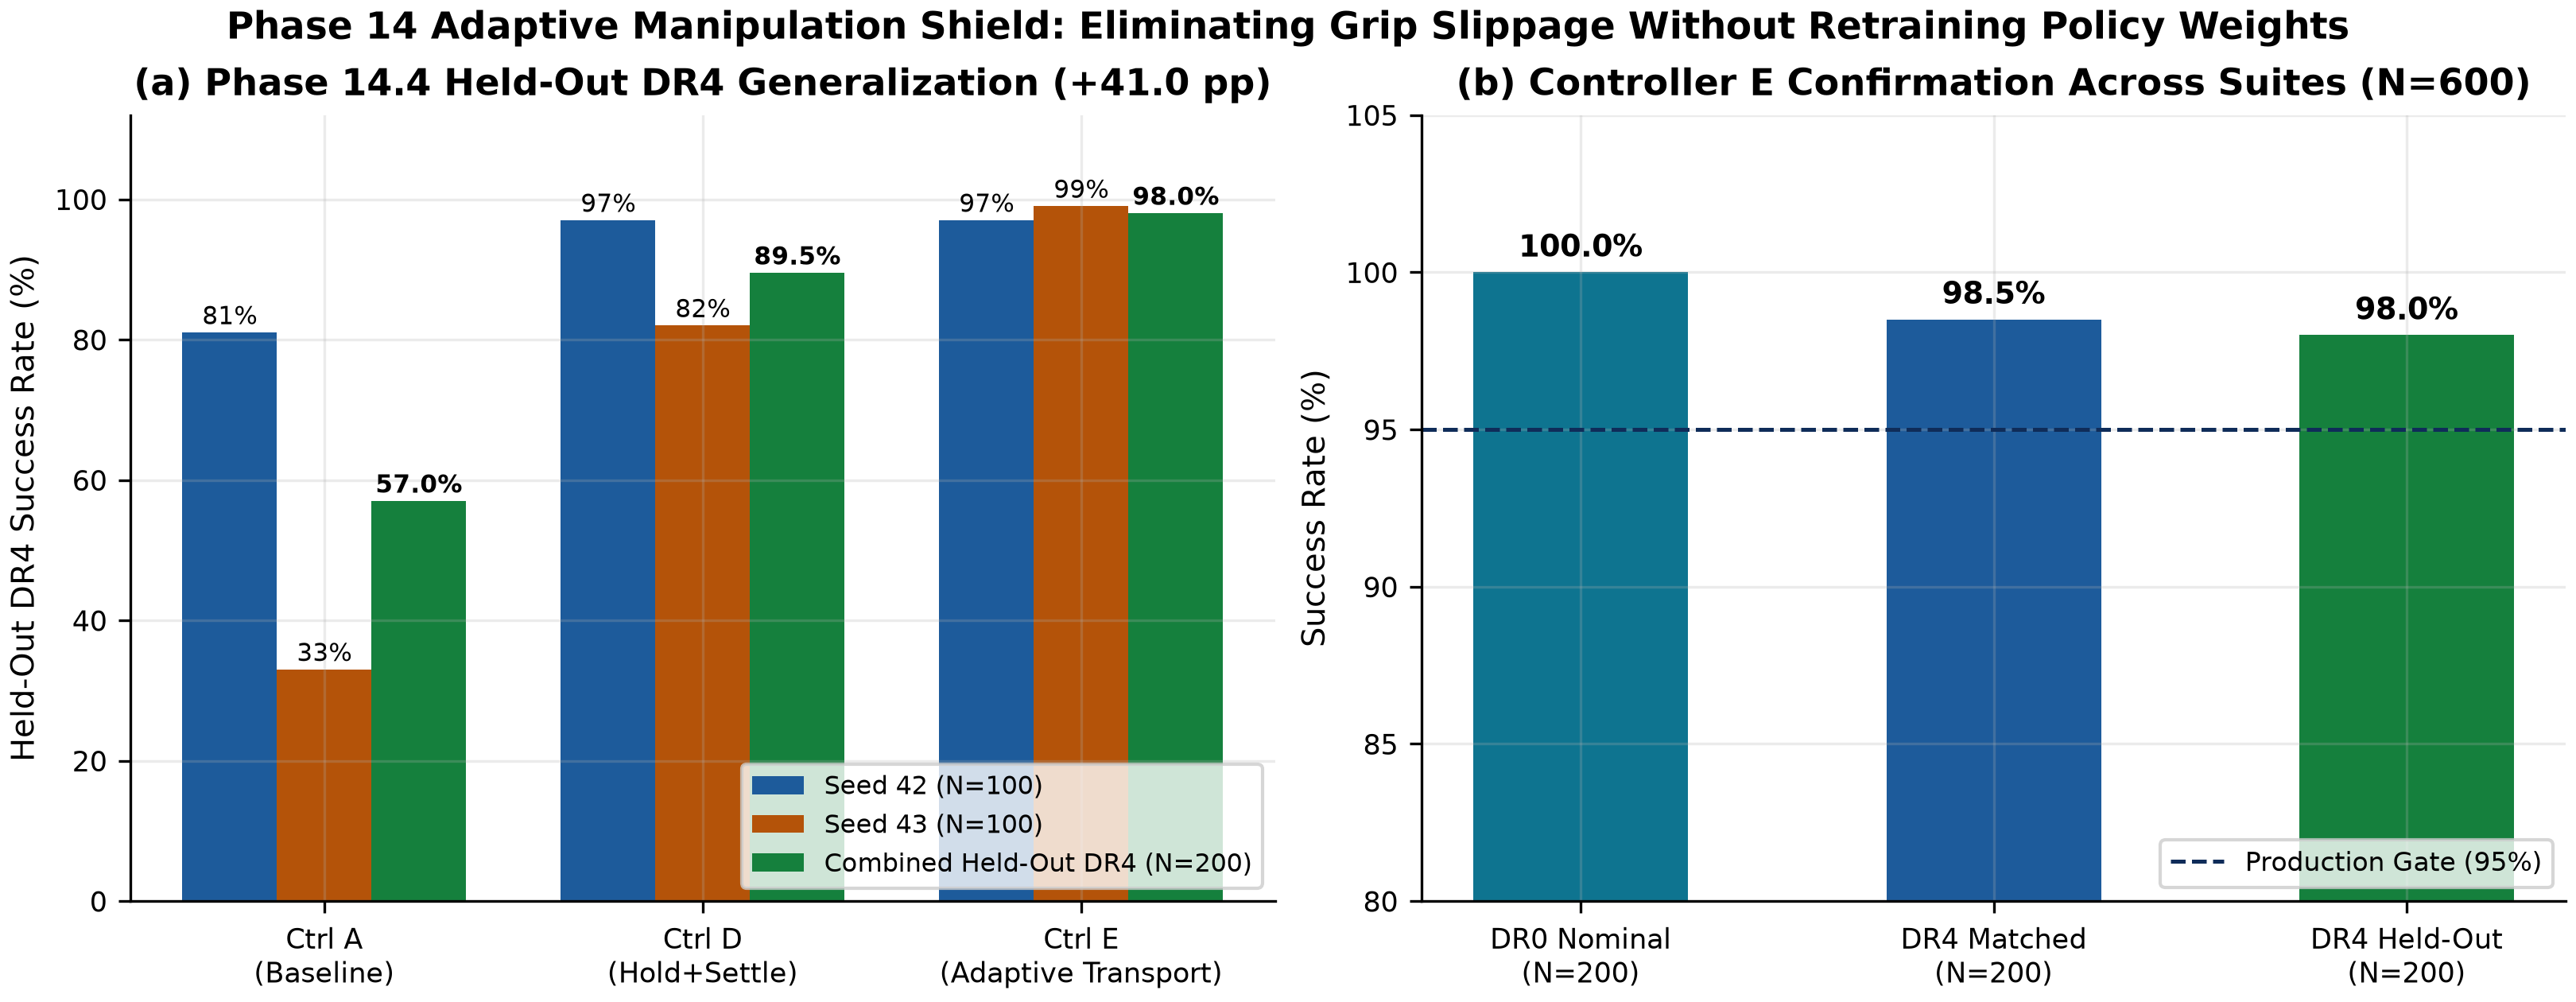
\includegraphics[width=0.92\linewidth]{publication/figures_2d/fig06_phase14_adaptive_controller_comparison.png}\caption{Figure 6.2: Phase 14.4 Held-Out DR4 generalization breakthrough (+41.0 pp) and suite-wide consistency.}\end{figure}
\section{6.3 Algorithm 3: Runtime Controller E \& Phase 14.3 Confirmation Comparisons}
\begin{quote}\small\textbf{Algorithm Summary}\\Algorithm 3: Controller E Adaptive Transport Shield (src/rl/adaptive\_controllers.py) \\ 1. Inspect live PyBullet contact points on finger links 9 \& 10: compute f9, f10 normal forces \& bilateral flag. \\ 2. If rel\_dist < grasp\_zone and cube\_z < 0.05m and not grasp\_settled: \\    clamp dx = 0, dy = 0, force gripper\_close, throttle dz = 0 for settle\_steps = 3 ticks. \\ 3. During LIFT \& TRANSPORT (cube\_z > table): monitor slip delta ||p\_obj - p\_ee|| and min(f9, f10). \\    Cap upward acceleration dz\_cmd <= dz\_safe(normal\_force, slippage) eliminating impulsive breakaway jerk. \\ 4. Forward stabilized 4D action directly to PyBulletSimulation without altering any neural policy weight.\end{quote}

\begin{longtable}{l l l l l l l l}\caption{Table 6.3: Phase 14.3 Seed-Level Controller A vs D Summary (results/phase14\_3/confirmation\_summary.csv)}\\\toprule
Seed & Controller & Regime & Success \% & Bilat \% & GBNL \% & Mean Slips & Mean Steps \\ \midrule \endhead
42 & A\_BASELINE & Nominal\_DR0 & 100.0\% & 100.0\% & 0.0\% & 0.01 & 15.9 \\
42 & A\_BASELINE & Matched\_DR4 & 100.0\% & 100.0\% & 0.0\% & 0.02 & 16.1 \\
42 & A\_BASELINE & Heldout\_DR4 & 81.0\% & 93.0\% & 18.0\% & 0.40 & 22.9 \\
43 & A\_BASELINE & Nominal\_DR0 & 95.0\% & 99.0\% & 3.0\% & 1.07 & 20.2 \\
43 & A\_BASELINE & Matched\_DR4 & 98.0\% & 99.0\% & 1.0\% & 0.60 & 19.3 \\
43 & A\_BASELINE & Heldout\_DR4 & 33.0\% & 62.0\% & 43.0\% & 4.90 & 36.3 \\
42 & D\_DUAL\_STAGE & Heldout\_DR4 & 97.0\% & 100.0\% & 3.0\% & 0.00 & 33.2 \\
42 & D\_DUAL\_STAGE & Nominal\_DR0 & 100.0\% & 100.0\% & 0.0\% & 0.01 & 16.9 \\
42 & D\_DUAL\_STAGE & Matched\_DR4 & 100.0\% & 100.0\% & 0.0\% & 0.01 & 17.2 \\
43 & D\_DUAL\_STAGE & Heldout\_DR4 & 82.0\% & 100.0\% & 1.0\% & 0.16 & 32.2 \\
43 & D\_DUAL\_STAGE & Nominal\_DR0 & 100.0\% & 100.0\% & 0.0\% & 0.35 & 20.9 \\
43 & D\_DUAL\_STAGE & Matched\_DR4 & 97.0\% & 99.0\% & 2.0\% & 0.39 & 20.8 \\
\bottomrule \end{longtable}
\begin{longtable}{l l l l l l l l}\caption{Table 6.2: Phase 14-Lite Controller A->E Slip \& Vertical Jerk Reduction (controller\_comparison.csv)}\\\toprule
Seed & Controller & Regime & Success & Grasp->Lift & Slips & Peak Jerk & GBNL \% \\ \midrule \endhead
COMBINED & A\_BASELINE & Nominal\_DR0 & 97.5\% & 98.5\% & 0.54 & 36.26 & 1.5\% \\
COMBINED & B\_ACCEL\_SMOOTHING & Nominal\_DR0 & 98.0\% & 99.0\% & 0.40 & 32.57 & 1.0\% \\
COMBINED & C\_SLIP\_AWARE & Nominal\_DR0 & 98.5\% & 99.5\% & 0.34 & 32.21 & 0.5\% \\
COMBINED & A\_BASELINE & Matched\_DR4 & 99.0\% & 99.5\% & 0.31 & 36.38 & 0.5\% \\
COMBINED & B\_ACCEL\_SMOOTHING & Matched\_DR4 & 99.5\% & 100.0\% & 0.38 & 32.36 & 0.0\% \\
COMBINED & C\_SLIP\_AWARE & Matched\_DR4 & 98.5\% & 99.5\% & 0.40 & 31.67 & 0.5\% \\
COMBINED & A\_BASELINE & Heldout\_DR4 & 57.0\% & 66.8\% & 2.65 & 56.85 & 30.5\% \\
COMBINED & B\_ACCEL\_SMOOTHING & Heldout\_DR4 & 55.0\% & 65.2\% & 2.56 & 56.23 & 32.0\% \\
COMBINED & C\_SLIP\_AWARE & Heldout\_DR4 & 57.5\% & 68.5\% & 2.35 & 56.25 & 29.0\% \\
42 & A\_BASELINE & Nominal\_DR0 & 100.0\% & 100.0\% & 0.01 & 25.66 & 0.0\% \\
42 & B\_ACCEL\_SMOOTHING & Nominal\_DR0 & 100.0\% & 100.0\% & 0.01 & 22.30 & 0.0\% \\
42 & C\_SLIP\_AWARE & Nominal\_DR0 & 100.0\% & 100.0\% & 0.01 & 22.32 & 0.0\% \\
42 & A\_BASELINE & Matched\_DR4 & 100.0\% & 100.0\% & 0.02 & 26.38 & 0.0\% \\
42 & B\_ACCEL\_SMOOTHING & Matched\_DR4 & 100.0\% & 100.0\% & 0.01 & 23.41 & 0.0\% \\
42 & C\_SLIP\_AWARE & Matched\_DR4 & 100.0\% & 100.0\% & 0.02 & 23.85 & 0.0\% \\
42 & A\_BASELINE & Heldout\_DR4 & 81.0\% & 82.0\% & 0.40 & 50.57 & 18.0\% \\
42 & B\_ACCEL\_SMOOTHING & Heldout\_DR4 & 81.0\% & 81.0\% & 0.38 & 49.72 & 19.0\% \\
42 & C\_SLIP\_AWARE & Heldout\_DR4 & 85.0\% & 86.0\% & 0.38 & 50.14 & 14.0\% \\
43 & A\_BASELINE & Nominal\_DR0 & 95.0\% & 97.0\% & 1.07 & 46.87 & 3.0\% \\
43 & B\_ACCEL\_SMOOTHING & Nominal\_DR0 & 96.0\% & 98.0\% & 0.79 & 42.85 & 2.0\% \\
43 & C\_SLIP\_AWARE & Nominal\_DR0 & 97.0\% & 99.0\% & 0.67 & 42.09 & 1.0\% \\
43 & A\_BASELINE & Matched\_DR4 & 98.0\% & 99.0\% & 0.60 & 46.39 & 1.0\% \\
43 & B\_ACCEL\_SMOOTHING & Matched\_DR4 & 99.0\% & 100.0\% & 0.75 & 41.31 & 0.0\% \\
43 & C\_SLIP\_AWARE & Matched\_DR4 & 97.0\% & 99.0\% & 0.77 & 39.50 & 1.0\% \\
43 & A\_BASELINE & Heldout\_DR4 & 33.0\% & 48.8\% & 4.90 & 63.13 & 43.0\% \\
43 & B\_ACCEL\_SMOOTHING & Heldout\_DR4 & 29.0\% & 46.4\% & 4.75 & 62.73 & 45.0\% \\
43 & C\_SLIP\_AWARE & Heldout\_DR4 & 30.0\% & 47.6\% & 4.32 & 62.35 & 44.0\% \\
\bottomrule \end{longtable}
\chapter{Chapter 7: Stress Testing, Multi-Object Pre-Grasp Sorting, Masked BC-SAC, and Assembly (Phase 15)}
\section{7.1 Phase 15.1 Perturbation Sensitivity Matrix (320 Episodes)}
Stress evaluation under observation noise, actuator delay, and unprivileged observations (Table 7.1) proved high resilience to Gaussian spatial noise (+-3 mm: 97.5\%, +-5 mm: 95.0\%), moderate tolerance to 1-step delay (72.5\%), total breakdown at >=2-step latency (0.0\%), and a drop to 42.5\% when ground-truth velocity/orientation cues were masked.

\begin{longtable}{l l l l l l}\caption{Table 7.1: Complete Phase 15.1 Readiness Stress Test Suite (results/phase15\_1/phase15\_1\_results.json)}\\\toprule
Scenario Condition & Group & Success & Delta vs Base & Grasp & Class \\ \midrule \endhead
A0\_CLEAN\_BASELINE & Baseline & 95.0\% & +0.0 pp & 100.0\% & A - ROBUST \\
A0\_CLEAN\_BASELINE & Baseline & 100.0\% & +0.0 pp & 100.0\% & A - ROBUST \\
A0\_CLEAN\_BASELINE & Baseline & 97.5\% & +0.0 pp & 100.0\% & A - ROBUST \\
A1\_NOISE\_3MM & Obs\_Noise & 100.0\% & +5.0 pp & 100.0\% & A - ROBUST \\
A1\_NOISE\_3MM & Obs\_Noise & 95.0\% & -5.0 pp & 100.0\% & A - ROBUST \\
A1\_NOISE\_3MM & Obs\_Noise & 97.5\% & +0.0 pp & 100.0\% & A - ROBUST \\
A2\_NOISE\_5MM & Obs\_Noise & 100.0\% & +5.0 pp & 100.0\% & A - ROBUST \\
A2\_NOISE\_5MM & Obs\_Noise & 90.0\% & -10.0 pp & 100.0\% & A - ROBUST \\
A2\_NOISE\_5MM & Obs\_Noise & 95.0\% & -2.5 pp & 100.0\% & A - ROBUST \\
B1\_OBS\_DELAY\_1 & Latency & 55.0\% & -40.0 pp & 95.0\% & C - FRAGILE \\
B1\_OBS\_DELAY\_1 & Latency & 90.0\% & -10.0 pp & 100.0\% & A - ROBUST \\
B1\_OBS\_DELAY\_1 & Latency & 72.5\% & -25.0 pp & 97.5\% & C - FRAGILE \\
B2\_OBS\_DELAY\_2 & Latency & 0.0\% & -95.0 pp & 25.0\% & D - FAILED \\
B2\_OBS\_DELAY\_2 & Latency & 0.0\% & -100.0 pp & 35.0\% & D - FAILED \\
B2\_OBS\_DELAY\_2 & Latency & 0.0\% & -97.5 pp & 30.0\% & D - FAILED \\
B3\_OBS\_DELAY\_4 & Latency & 0.0\% & -95.0 pp & 0.0\% & D - FAILED \\
B3\_OBS\_DELAY\_4 & Latency & 0.0\% & -100.0 pp & 10.0\% & D - FAILED \\
B3\_OBS\_DELAY\_4 & Latency & 0.0\% & -97.5 pp & 5.0\% & D - FAILED \\
B4\_COMBINED\_DELAY\_1\_1 & Latency & 0.0\% & -95.0 pp & 40.0\% & D - FAILED \\
B4\_COMBINED\_DELAY\_1\_1 & Latency & 0.0\% & -100.0 pp & 30.0\% & D - FAILED \\
B4\_COMBINED\_DELAY\_1\_1 & Latency & 0.0\% & -97.5 pp & 35.0\% & D - FAILED \\
C1\_UNPRIVILEGED & Contact\_Mode & 45.0\% & -50.0 pp & 100.0\% & D - FAILED \\
C1\_UNPRIVILEGED & Contact\_Mode & 40.0\% & -60.0 pp & 100.0\% & D - FAILED \\
C1\_UNPRIVILEGED & Contact\_Mode & 42.5\% & -55.0 pp & 100.0\% & D - FAILED \\
\bottomrule \end{longtable}
\section{7.2 Phase 15.2 \& 15.3: Multi-Object Sorting Gates, Vertical Approach Conditioning, and Assembly}
Phase 15.2.4 exposed ERR-005 (un-gated dense sorting suffered 163.2 collisions/ep and 0\% grasp). Phase 15.2.5A resolved this via 5-check bilateral grasp gating in PreGraspController, yielding 50/50 (100\%) scripted 2-object sorting in 76.4 mean steps. On single-object RL (PandaSinglePreGraspEnv), resolving ERR-006 (adding continuous vertical potential Equation (11)) and ERR-007 (removing closed-gripper HOLD\_AT\_GOAL bias via masked BC Equations (12)-(13)) propelled pure BC (5B7) to 75\% grasp / 45\% lift and Hybrid BC-SAC (5B8) to 66\% grasp / 26\% lift, compared against 7\% lift for pure SAC (5B2). Full 28D->43D multi-object RL transfer (Phase 15.2.5C) remained BLOCKED. In Phase 15.3 peg-in-slot assembly, scripted baseline achieved 56.67\% insertion (1.41 deg align), while BC achieved 23.33\% pre-align / 0\% insertion. Phase 15 closed with 111/111 tests passing in 29.47 s.

\begin{figure}[htbp]\centering
\includegraphics[width=0.92\linewidth]{publication/equations/eq_11.png}\caption{Equation (11): Continuous vertical potential Phi\_z eliminating z=0.50m hover deadlocks.}\end{figure}
\begin{figure}[htbp]\centering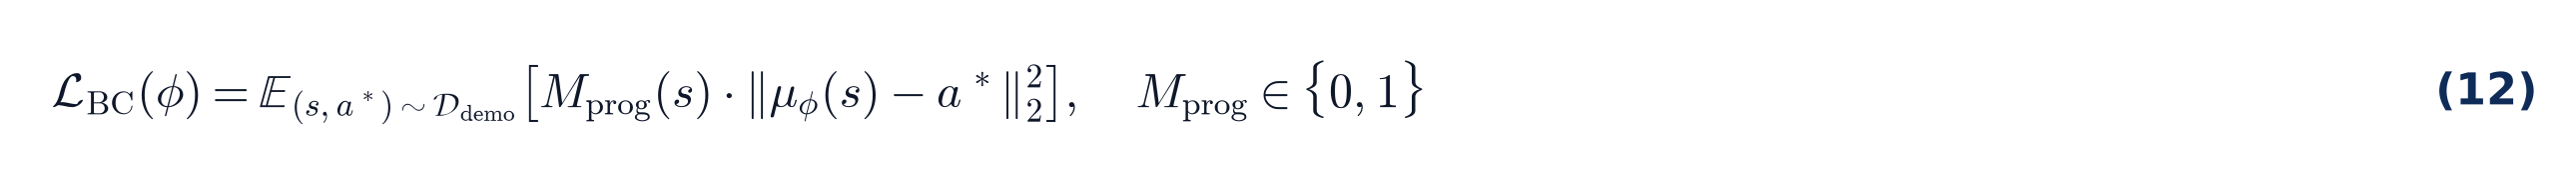
\includegraphics[width=0.92\linewidth]{publication/equations/eq_12.png}\caption{Equation (12): Progress-masked Behavioral Cloning L2 regression loss.}\end{figure}
\begin{figure}[htbp]\centering
\includegraphics[width=0.92\linewidth]{publication/equations/eq_13.png}\caption{Equation (13): Exponentially decaying Hybrid BC-SAC objective.}\end{figure}
\begin{figure}[htbp]\centering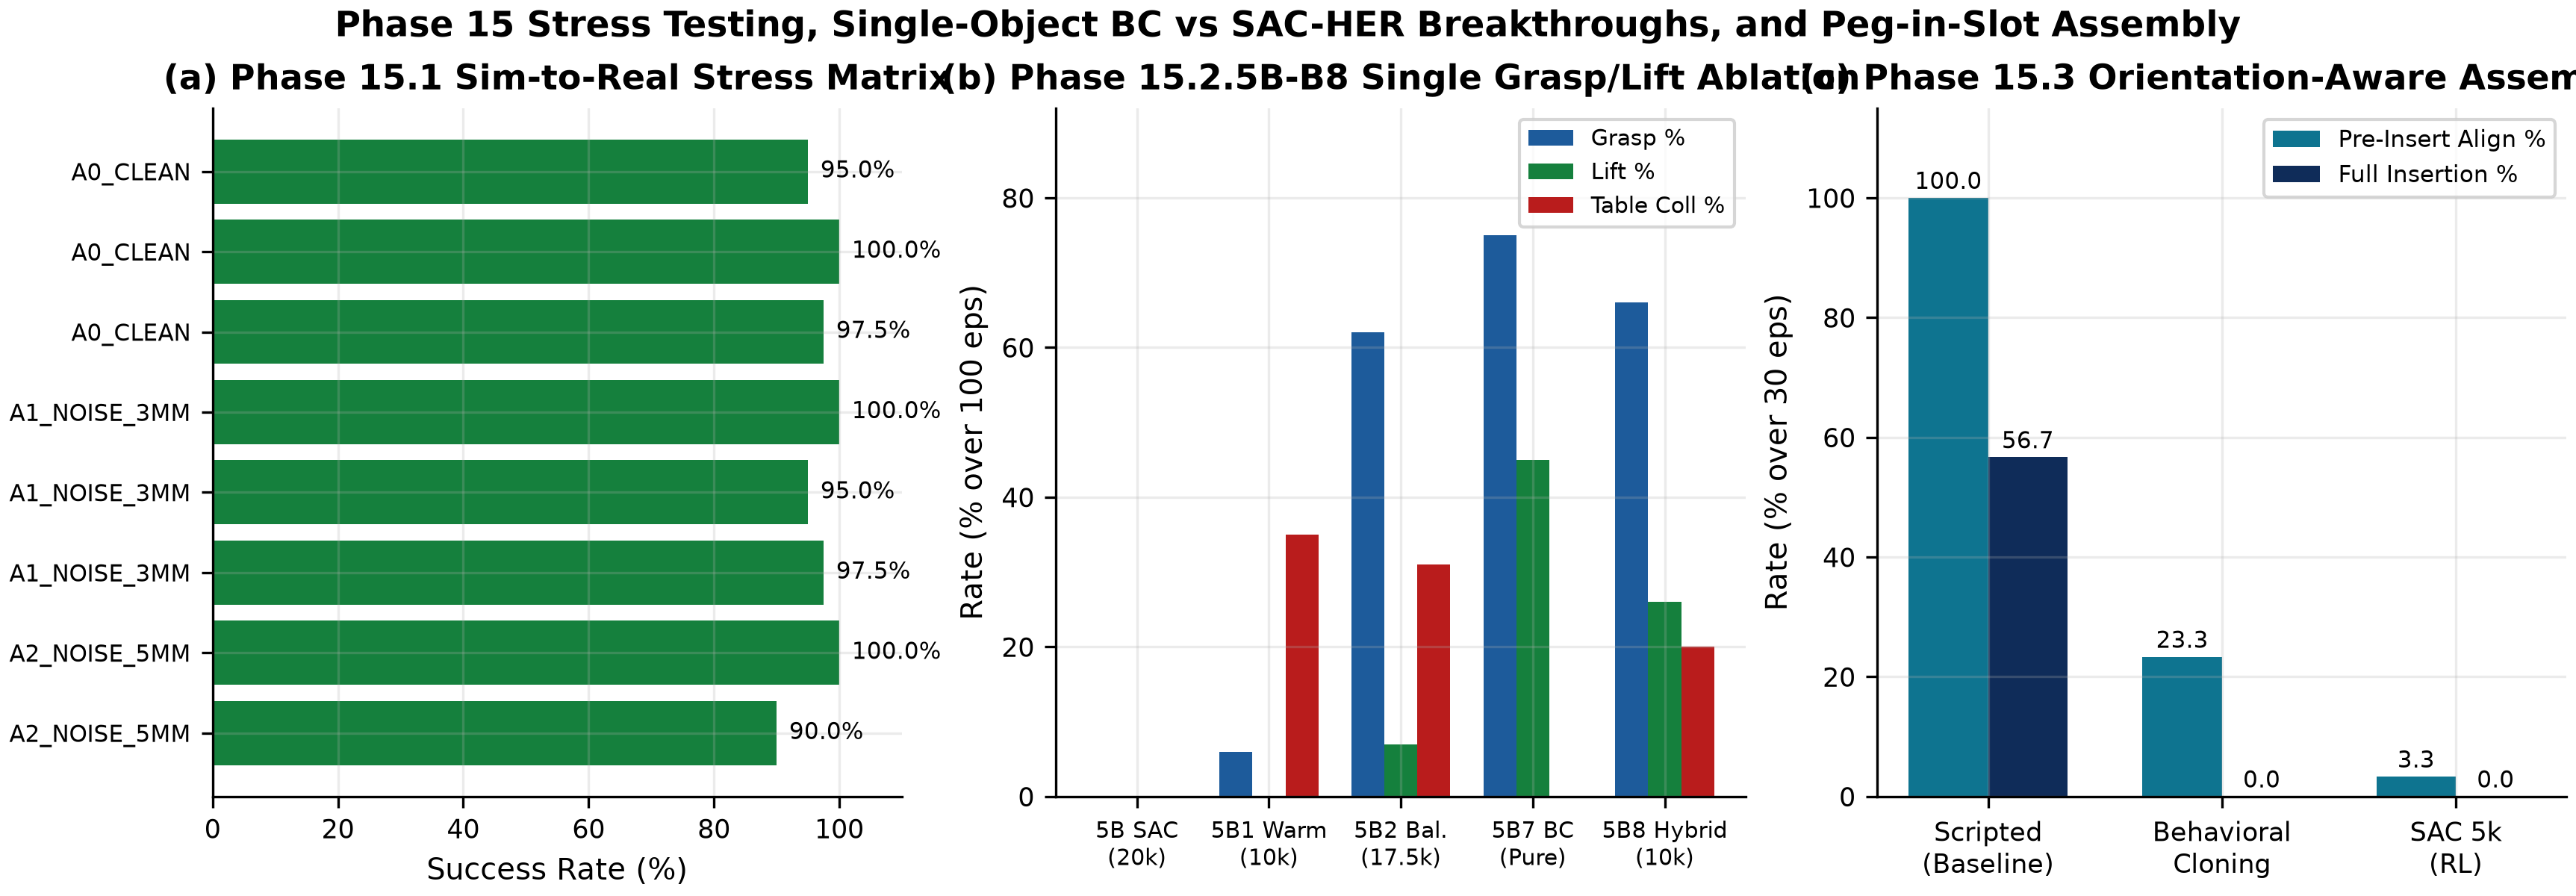
\includegraphics[width=0.92\linewidth]{publication/figures_2d/fig07_phase15_grasp_bc_vs_sac_ablations.png}\caption{Figure 7.1: Phase 15.1 stress resilience, 15.2.5B-B8 grasp/lift ablations, and Phase 15.3 assembly benchmark.}\end{figure}
\section{7.4 PreGrasp Gate, Masked BC-SAC Algorithms, and Robustness/Assembly Audits}
\begin{quote}\small\textbf{Algorithm Summary}\\Algorithm 4: Phase 15.2.5A Five-Check Bilateral Grasp Authorization Gate \\ Authorize gripper closing ONLY when ALL 5 physical conditions hold simultaneously: \\   C1: xy\_err(EE, obj) <= 0.015 m  AND  C2: |z\_ee - z\_grasp| <= 0.018 m \\   C3: finger\_width > 0.065 m (open descent prevents top-knocking collision) \\   C4: ||v\_obj|| < 0.02 m/s (cube stationary)  AND  C5: active target object locked. \\  \\ Algorithm 5: Progress-Masked Hybrid BC-SAC (Phase 15.2.5B7 / 5B8) \\ 1. Filter demo buffer using binary progress mask M\_prog(s) = 0 on trailing HOLD\_AT\_GOAL frames (removing 78\% closed bias). \\ 2. Pretrain actor via masked L2 loss Eq. (12) for pure BC baseline (75\% grasp / 45\% lift, 0\% coll). \\ 3. Anneal BC auxiliary weight lambda\_BC(t) = lambda\_0 * exp(-kappa * t) alongside SAC Eq. (13) with entropy floor.\end{quote}

\begin{longtable}{l l l l l l}\caption{Table 7.2: Phase 15 Phase-3 PickPlace DR Cross-Perturbation Results (phase15\_phase3\_robustness\_results.json)}\\\toprule
Model & Condition & Eps & Success \% & Grasp \% & Lift \% \\ \midrule \endhead
DR4\_Seed42 & DR1\_POS & 20 & 100.0\% & 100.0\% & 70.0\% \\
DR4\_Seed42 & DR2\_POSE\_TARGET & 20 & 100.0\% & 100.0\% & 80.0\% \\
DR4\_Seed42 & DR4\_FULL\_PHYSICS & 20 & 95.0\% & 100.0\% & 50.0\% \\
DR4\_Seed42 & DR4\_OBS\_NOISE\_5MM & 20 & 100.0\% & 100.0\% & 60.0\% \\
DR4\_Seed42 & DR4\_OBS\_DELAY\_1 & 20 & 95.0\% & 100.0\% & 80.0\% \\
DR4\_Seed43 & DR1\_POS & 20 & 100.0\% & 100.0\% & 70.0\% \\
DR4\_Seed43 & DR2\_POSE\_TARGET & 20 & 90.0\% & 95.0\% & 75.0\% \\
DR4\_Seed43 & DR4\_FULL\_PHYSICS & 20 & 95.0\% & 100.0\% & 60.0\% \\
DR4\_Seed43 & DR4\_OBS\_NOISE\_5MM & 20 & 95.0\% & 100.0\% & 65.0\% \\
DR4\_Seed43 & DR4\_OBS\_DELAY\_1 & 20 & 65.0\% & 100.0\% & 50.0\% \\
\bottomrule \end{longtable}
\begin{longtable}{l l l l l l}\caption{Table 7.3: Phase 15.3 Orientation-Aware Peg-in-Slot Assembly Benchmark (30 Eps Each)}\\\toprule
Policy Variant & Eps & Grasp \% & Pre-Insert Align \% & Full Insertion \% & Mean Angle Err \\ \midrule \endhead
Scripted Baseline & 30 & 100.0\% & 100.0\% & 56.67\% & 1.41 deg \\
bc\_warmstart\_only & 30 & 23.3\% & 6.67\% & 0.00\% & 84.60 deg \\
sac\_her\_2500 & 30 & 6.7\% & 0.00\% & 0.00\% & 84.57 deg \\
sac\_her\_5000 & 30 & 3.3\% & 0.00\% & 0.00\% & 80.92 deg \\
\bottomrule \end{longtable}
\chapter{Chapter 8: Hierarchical RL, Oblique RGB-D Vision, Dynamic Tracking, and Compliant Assembly (Phase 16)}
\section{8.1 Hierarchical Option-Critic, Oblique 128x128 RGB-D Perception, and Dynamic Kalman Control}
Phase 16 expanded manipulation along five fronts: (16.1) Five-skill SMDP option decomposition (Equation (14)) solving 30.0\% PickPlace at 12k steps after fixing ERR-008/009/010 vs 0.0\% Flat SAC; (16.2) Repositioning SimulatedRGBDCamera obliquely at (0.92, 0.28, 0.45) to overcome ERR-011 overhead self-occlusion, raising detection from 18.65\% to 99.9-100.0\% and clipping unprojection error to 14.81-15.55 mm (Equation (15), Figure 8.1, Table 8.1); (16.3) Constant-velocity Kalman target tracking (Equation (16)) reaching 95-100\% dynamic interception across moving cubes, sinusoids, and disturbances (Table 8.2); (16.4) Wall-force impedance compliance (Equation (17)) raising peg-in-slot assembly from 50.0\% to 53.33\%; and (16.6) Autonomous HRL 2-object evaluation yielding 25.0\% Object-1 / 0.0\% 2-object completion across 229 replans and 1,049 safety clamps.

\begin{figure}[htbp]\centering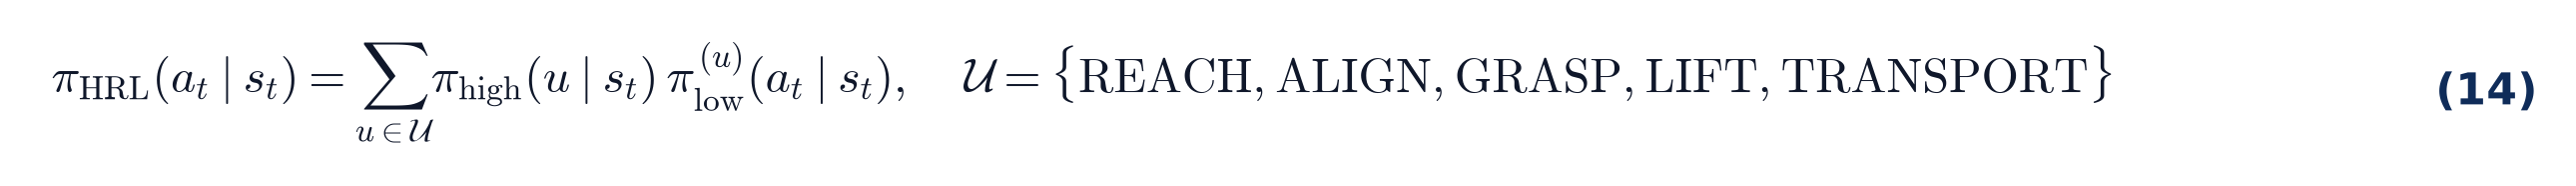
\includegraphics[width=0.92\linewidth]{publication/equations/eq_14.png}\caption{Equation (14): Option-Critic five-skill hierarchical action policy.}\end{figure}
\begin{figure}[htbp]\centering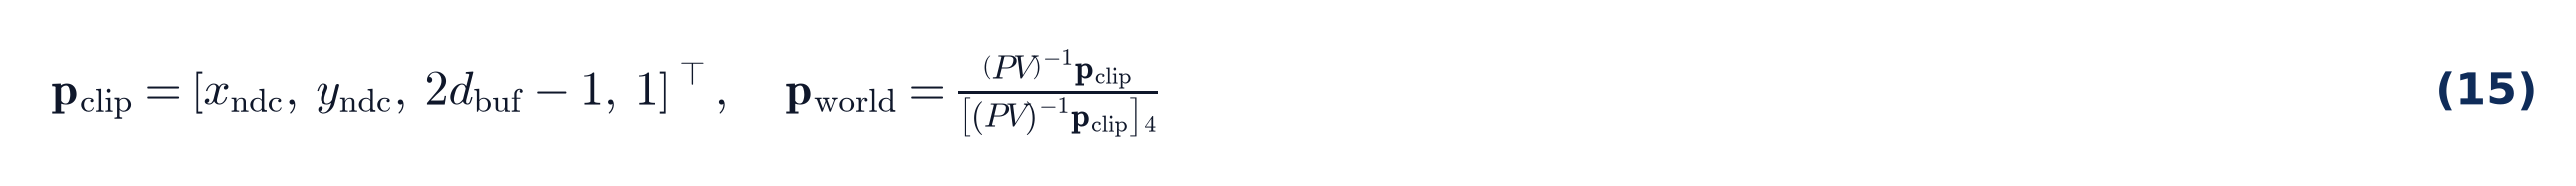
\includegraphics[width=0.92\linewidth]{publication/equations/eq_15.png}\caption{Equation (15): Inverse projection from clip-space depth buffer to world XYZ coordinates.}\end{figure}
\begin{figure}[htbp]\centering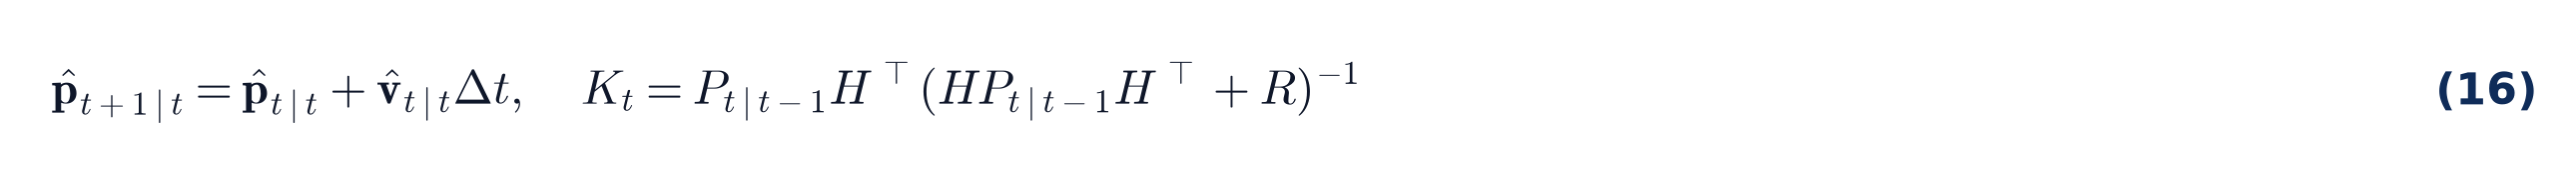
\includegraphics[width=0.92\linewidth]{publication/equations/eq_16.png}\caption{Equation (16): Discrete Kalman predictor and innovation gain update.}\end{figure}
\begin{figure}[htbp]\centering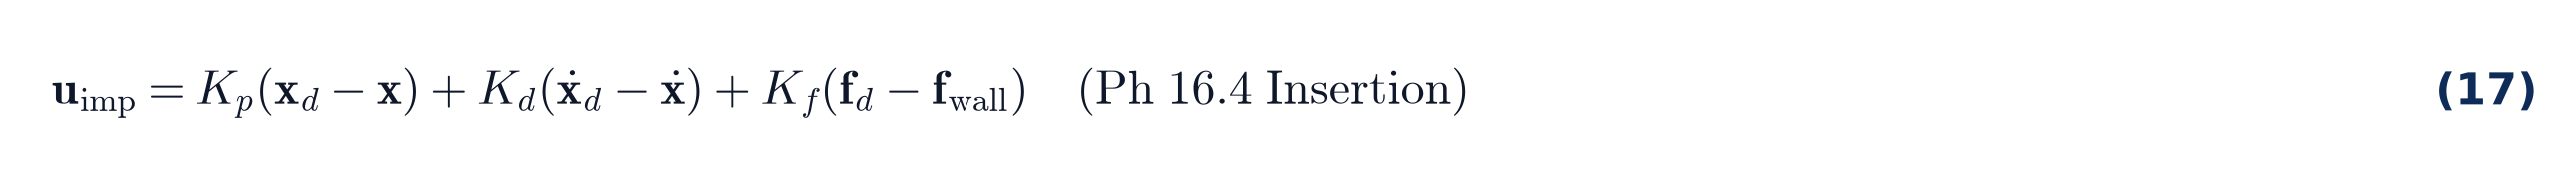
\includegraphics[width=0.92\linewidth]{publication/equations/eq_17.png}\caption{Equation (17): Cartesian compliant wall-force insertion law (Phase 16.4).}\end{figure}
\begin{figure}[htbp]\centering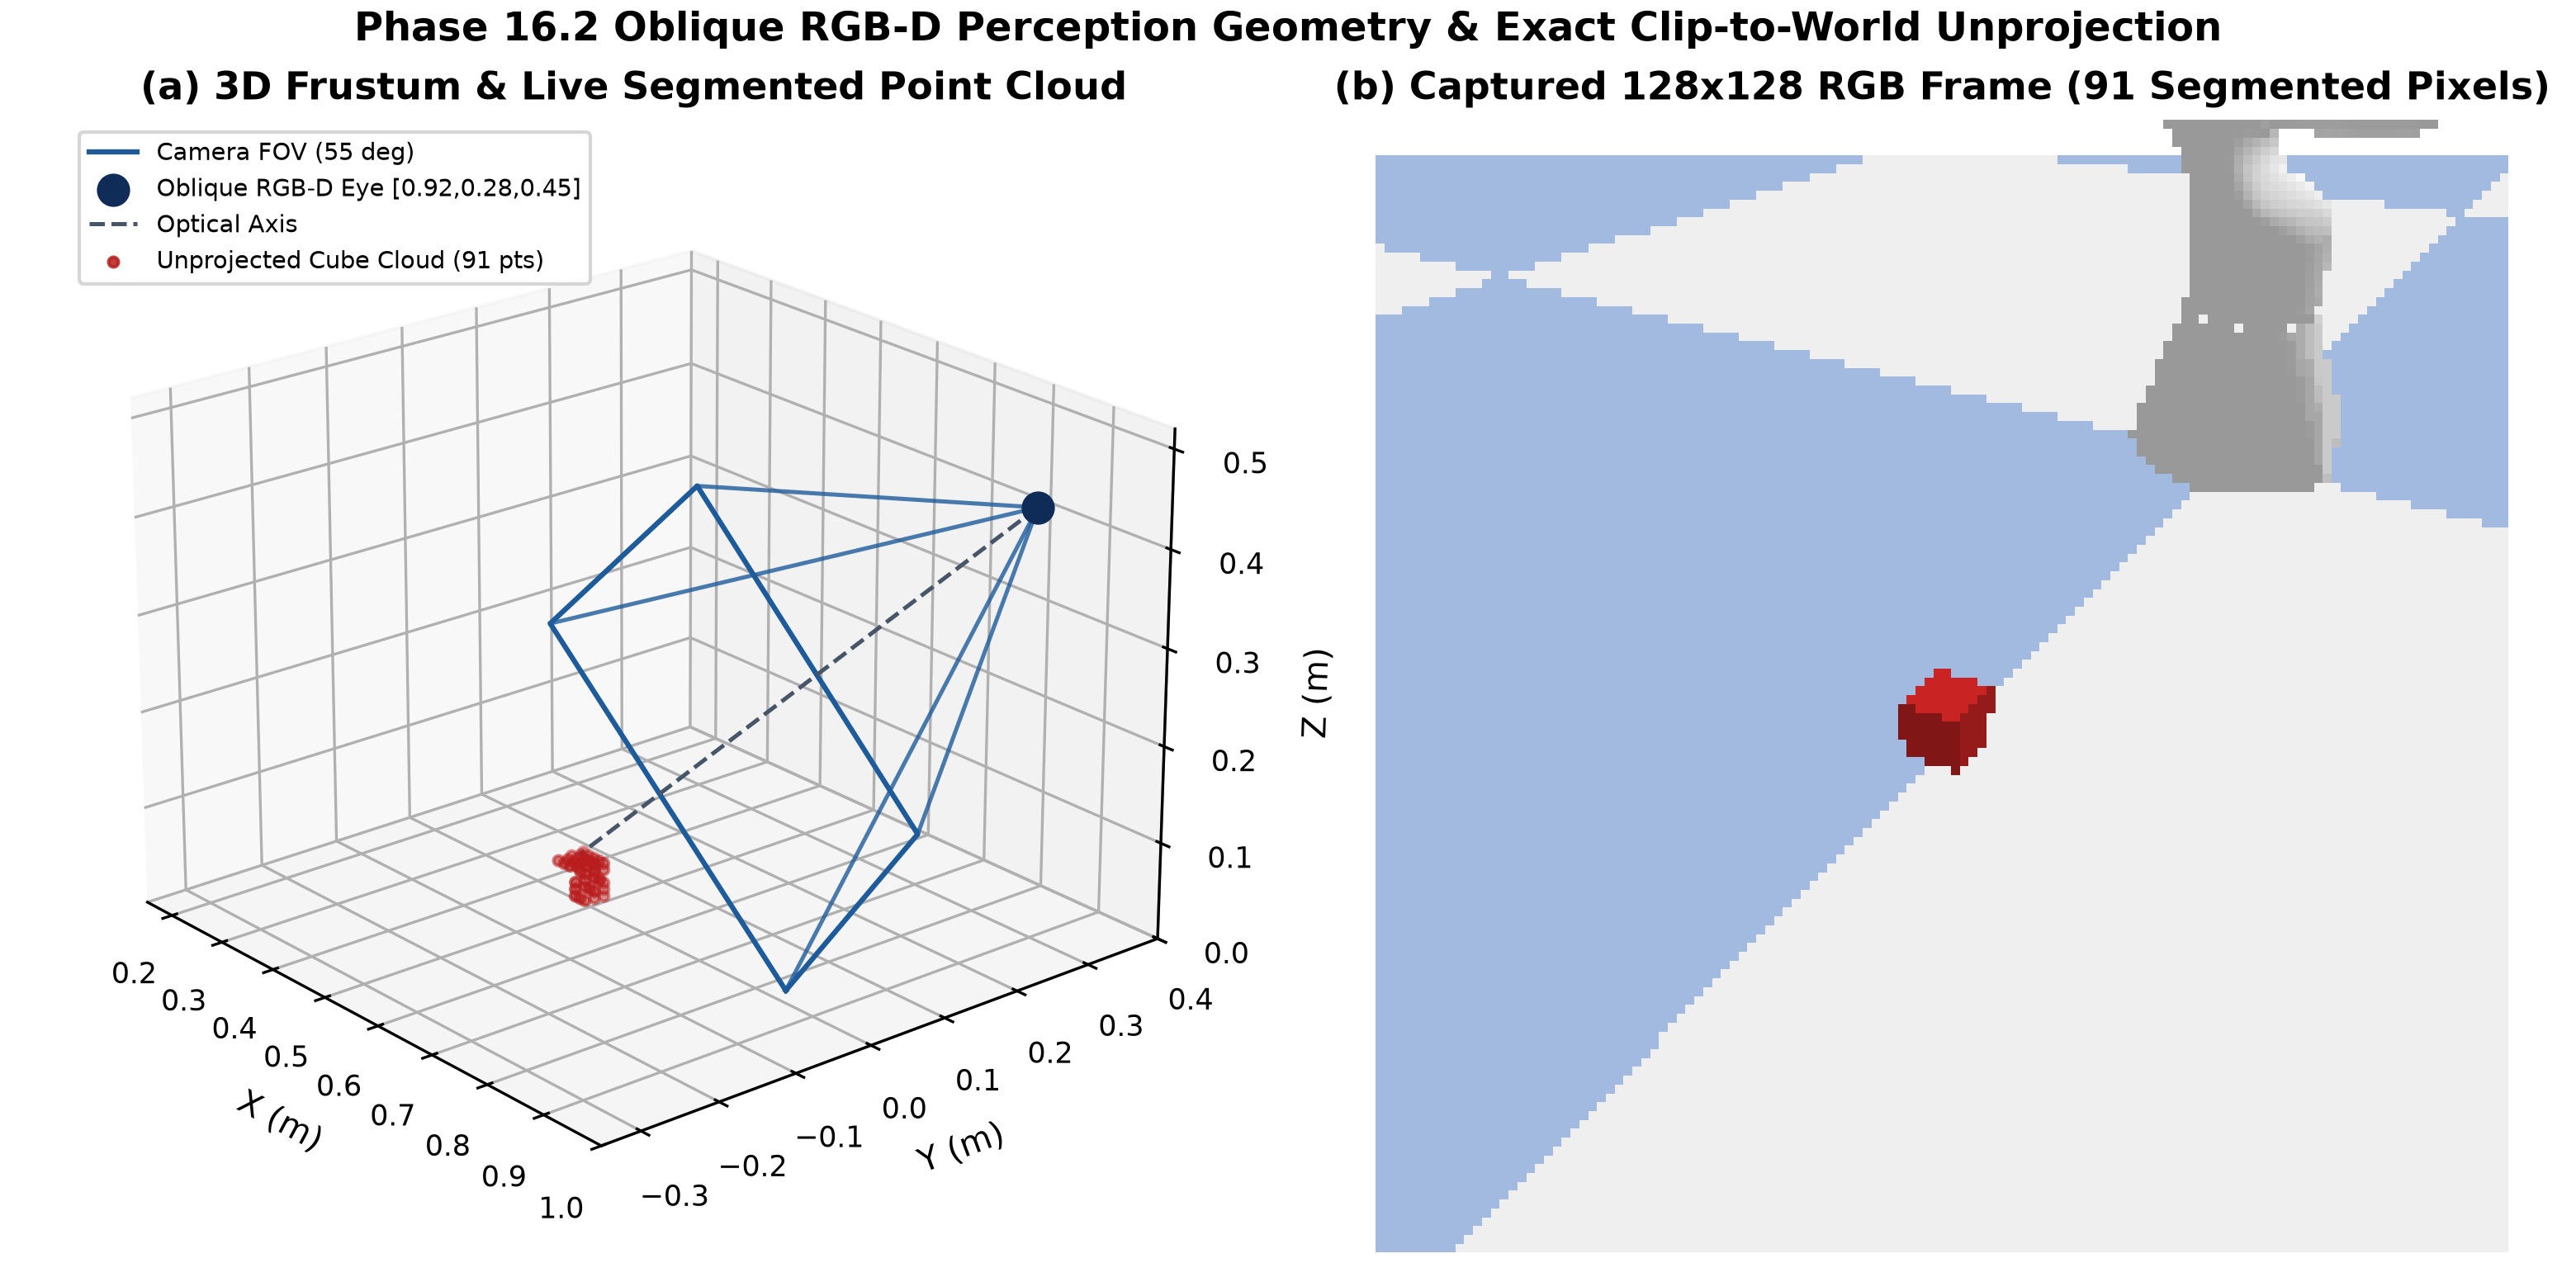
\includegraphics[width=0.92\linewidth]{publication/figures_3d/fig3d_03_oblique_rgbd_frustum_and_mujoco_workspace.png}\caption{Figure 8.1: Live PyBullet 3D oblique RGB-D frustum (55 deg FOV) and unprojected 91-pixel segmented cube cloud.}\end{figure}
\begin{longtable}{l l l l l l l}\caption{Table 8.1: Phase 16.2 Vision vs Privileged State Evaluation (phase16\_2\_vision\_results.json)}\\\toprule
Agent Variant & Obs Source & Grasp \% & Place \% & Colls & 3D Loc Err & Seg IoU \\ \midrule \endhead
SAC\_Privileged\_GT & PRIVILEGED\_GT\_STATE & 100.0\% & 100.0\% & 0.05 & GT Oracle & N/A \\
SAC\_RGBD\_Vision & RGBD\_VISION & 60.0\% & 15.0\% & 0.45 & 15.55 mm & 0.9983 \\
HRL\_Privileged\_GT & PRIVILEGED\_GT\_STATE & 40.0\% & 40.0\% & 3.90 & GT Oracle & N/A \\
HRL\_RGBD\_Vision & RGBD\_VISION & 25.0\% & 20.0\% & 1.55 & 14.81 mm & 0.9999 \\
\bottomrule \end{longtable}
\begin{longtable}{l l l l l l l}\caption{Table 8.2: Phase 16.3 Dynamic Moving Target \& Disturbance Results (phase16\_3\_dynamic\_results.json)}\\\toprule
Motion Mode & Speed & Predictive & Grasp \% & Success \% & Pred Err & Replans \\ \midrule \endhead
linear\_no\_prediction & 0.045 m/s & False & 100.0\% & 95.0\% & 31.38 mm & 1068 \\
linear\_predictive & 0.045 m/s & True & 100.0\% & 100.0\% & 33.45 mm & 1133 \\
sinusoidal\_predictive & 0.045 m/s & True & 100.0\% & 95.0\% & 34.89 mm & 1185 \\
disturbance\_step\_predictive & 0.035 m/s & True & 100.0\% & 95.0\% & 32.45 mm & 1141 \\
moving\_target\_and\_cube & 0.035 m/s & True & 100.0\% & 100.0\% & 33.81 mm & 1150 \\
\bottomrule \end{longtable}
\begin{figure}[htbp]\centering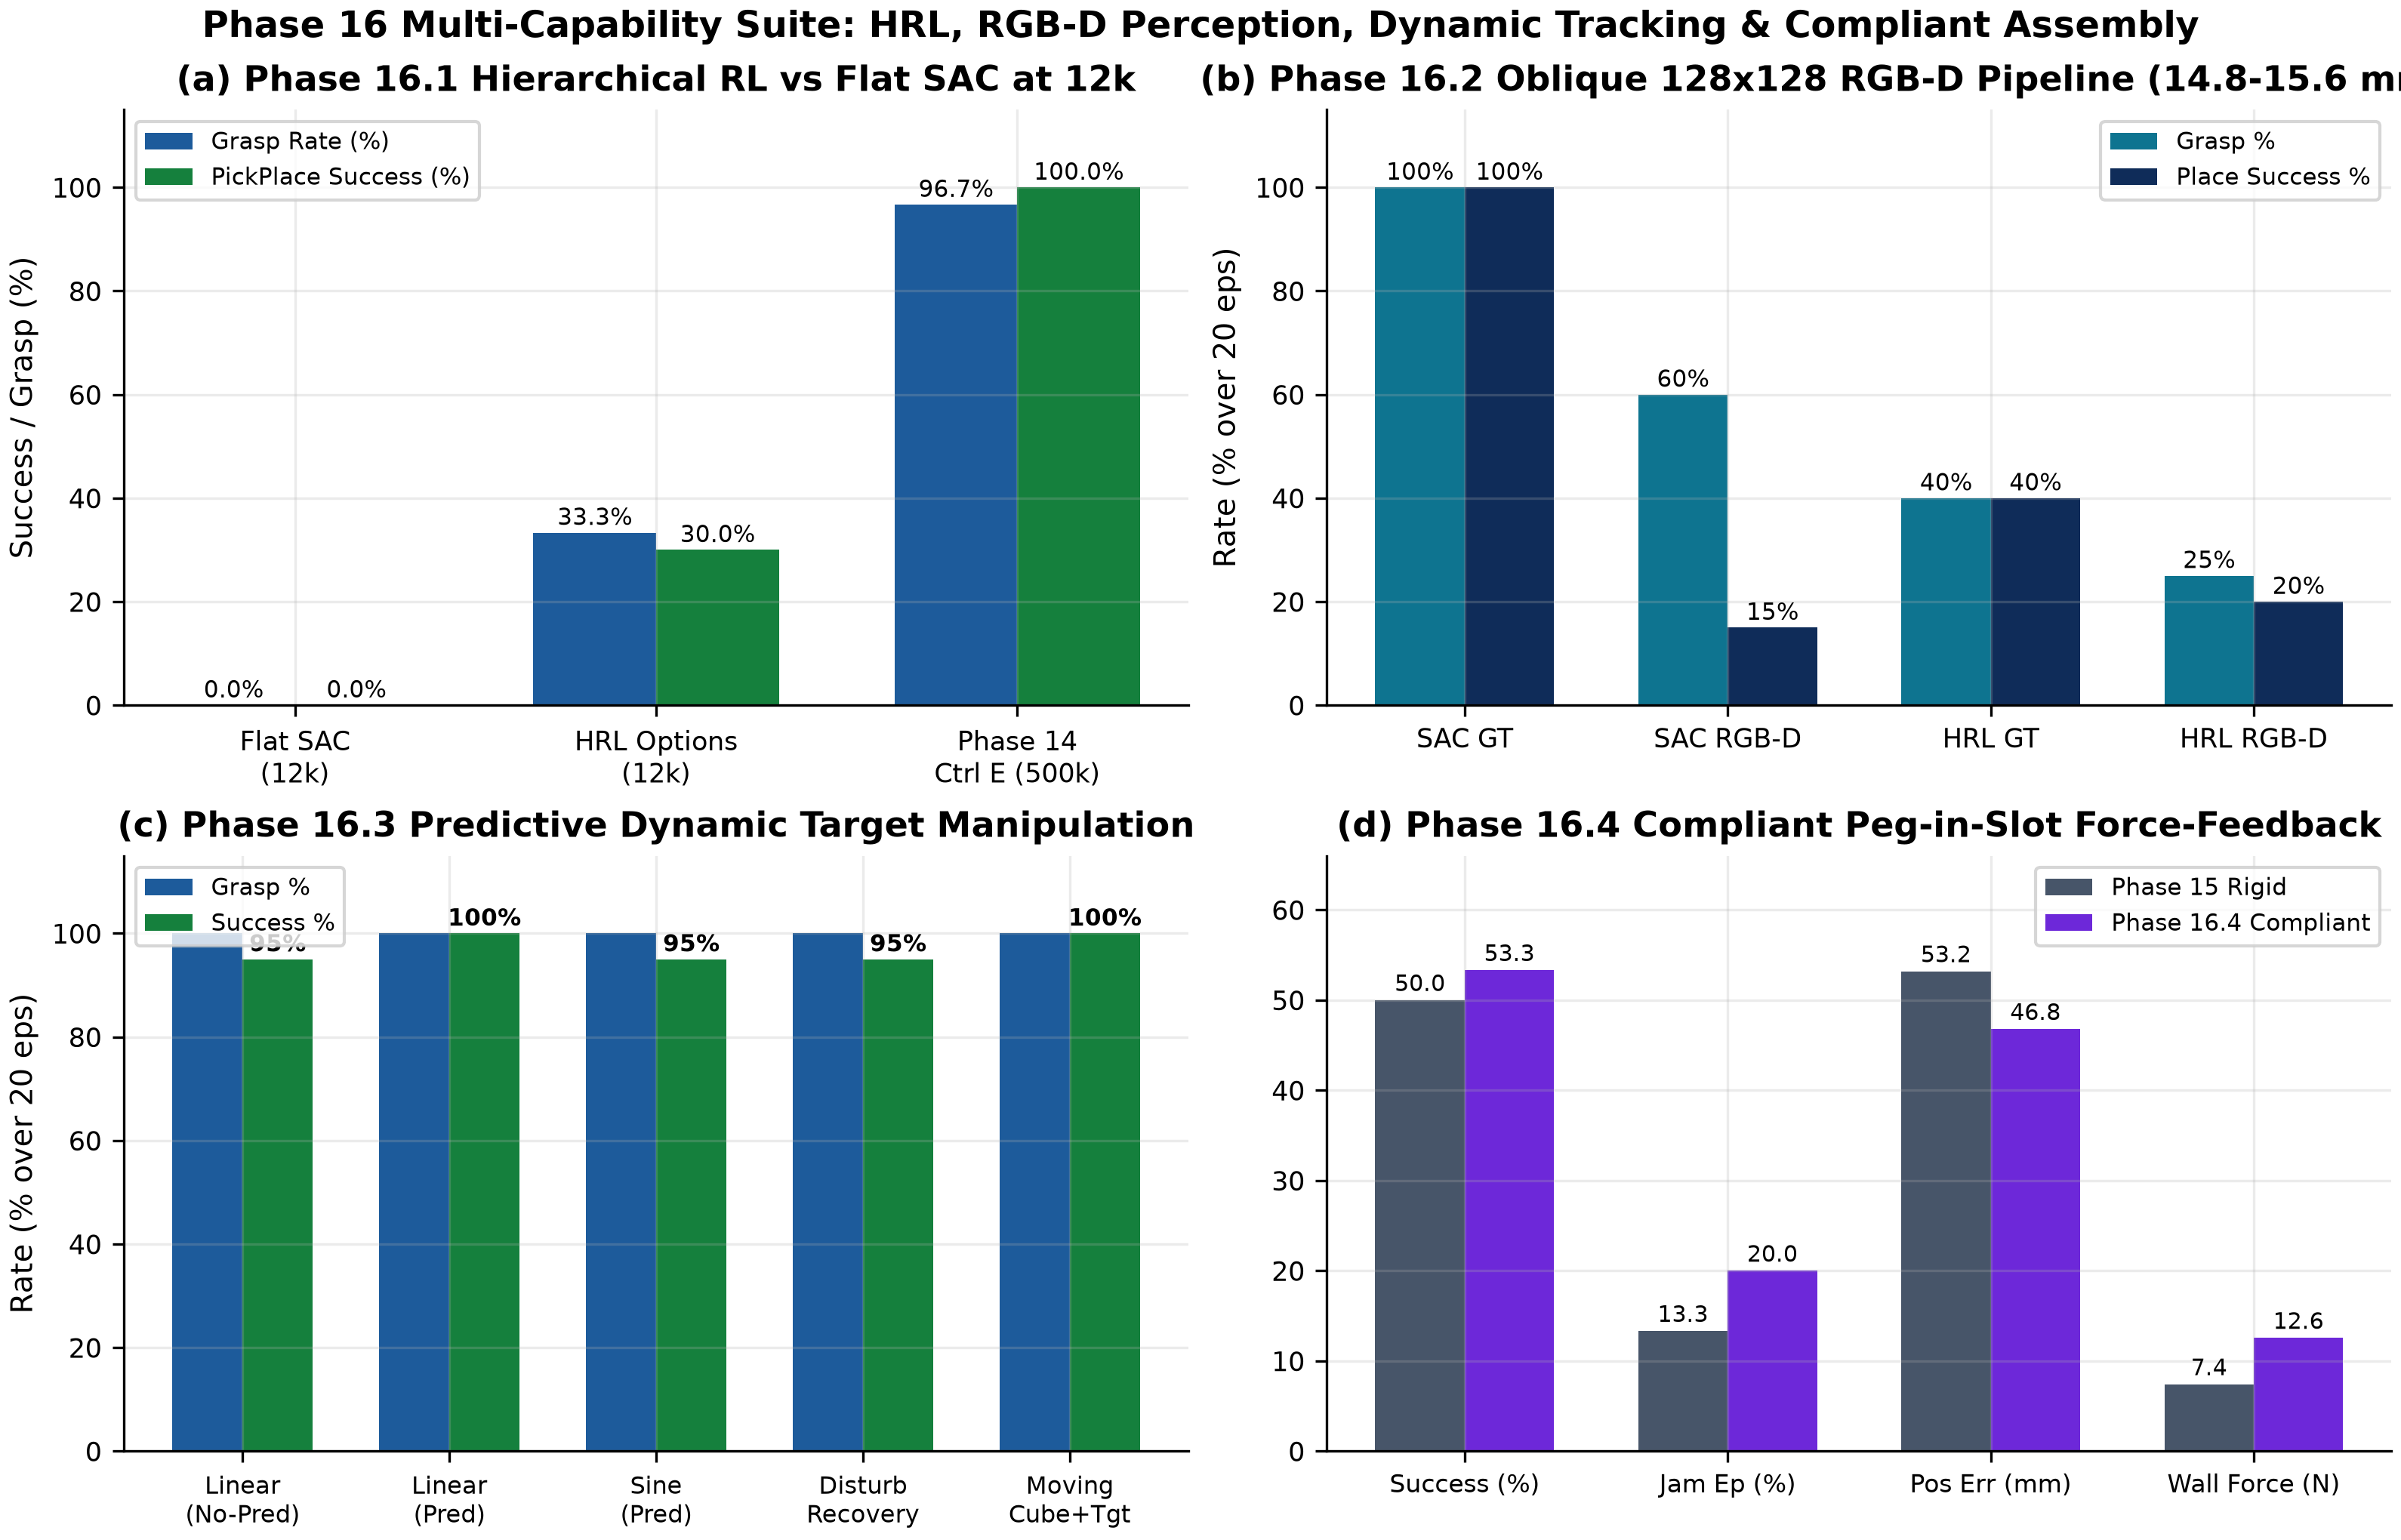
\includegraphics[width=0.92\linewidth]{publication/figures_2d/fig08_phase16_hrl_vision_dynamic_contact.png}\caption{Figure 8.2: Phase 16 comparative benchmarks across HRL, RGB-D vision, dynamic Kalman tracking, and compliant assembly.}\end{figure}
\section{8.4 HRL Option Selection \& Unprojected Oblique Vision Mechanics}
\begin{quote}\small\textbf{Algorithm Summary}\\Algorithm 6: Phase 16.1 SMDP 5-Skill Option-Critic Loop (src/hrl/hrl\_agent.py) \\ 1. High-level selector pi\_high(u | s\_t) picks active skill u in {REACH, ALIGN, GRASP, LIFT, TRANSPORT}. \\ 2. Run low-level skill policy a\_t ~ pi\_low^(u)(s\_t) until termination head beta\_u(s\_{t+k}) > 0.5 or max\_horizon. \\ 3. Assign bounded SMDP option reward using potential height delta 1.5*(h\_{t+k} - h\_t) + sparse completion +6.0. \\  \\ Algorithm 7: Phase 16.2 Oblique RGB-D Unprojection + Phase 16.3 Kalman Predictor \\ 1. Render 128x128 RGB + metric depth from oblique eye (0.92, 0.28, 0.45) avoiding Franka arm self-occlusion. \\ 2. Segment cube mask in HSV space (IoU 0.9983-0.9999) and unproject masked depth pixels via (PV)^(-1) Eq. (15). \\ 3. Pass centroid [x\_est, y\_est, z\_est] into 4-state constant-velocity Kalman filter Eq. (16) for moving-target interception.\end{quote}

\begin{longtable}{l l l l l}\caption{Table 8.3: Phase 16.1 Low-Level Option Policy \& Termination Head Training Accuracy}\\\toprule
Option Skill & Demo Samples & Actor MSE & Term BCE & Termination Acc \\ \midrule \endhead
REACH & 660 & 0.004779 & 0.005946 & 100.00\% \\
ALIGN & 180 & 0.011022 & 0.358004 & 74.44\% \\
GRASP & 384 & 0.023815 & 0.067245 & 100.00\% \\
LIFT & 540 & 0.002637 & 0.012431 & 100.00\% \\
TRANSPORT & 594 & 0.006278 & 0.083425 & 99.66\% \\
PLACE & 182 & 0.014696 & 0.244255 & 90.11\% \\
\bottomrule \end{longtable}
\chapter{Chapter 9: Cross-Simulator Validation (MuJoCo 4.0.1), Safety Envelope, and Hardware Boundary (Phase 17)}
\section{9.1 Cross-Engine Verification and Stress Suite Results}
After repairing massless dummy links in MJCF (ERR-012), Phase 17.1 measured zero-shot PyBullet->MuJoCo 4.0.1 transfer of Seed 42: 40.0\% bilateral contact, 5.0\% grasp, 0.0\% completion, rising to 50.0\% contact / 15.0\% grasp / 5.0\% completion after calibrating PD gains and tabletop Z offset (9.4 mm physics discrepancy). Phase 17.2 validated SafetySupervisor bounds (Equation (18)) across scenarios S1-S6 (Table 9.1) and confirmed 32.41 us E-stop cutoff across 250 faulty commands. Phase 17.3 physical robot execution was NOT\_ATTEMPTED; repository suite verification stands at 122/122 passed tests in 42.47 s.

\begin{figure}[htbp]\centering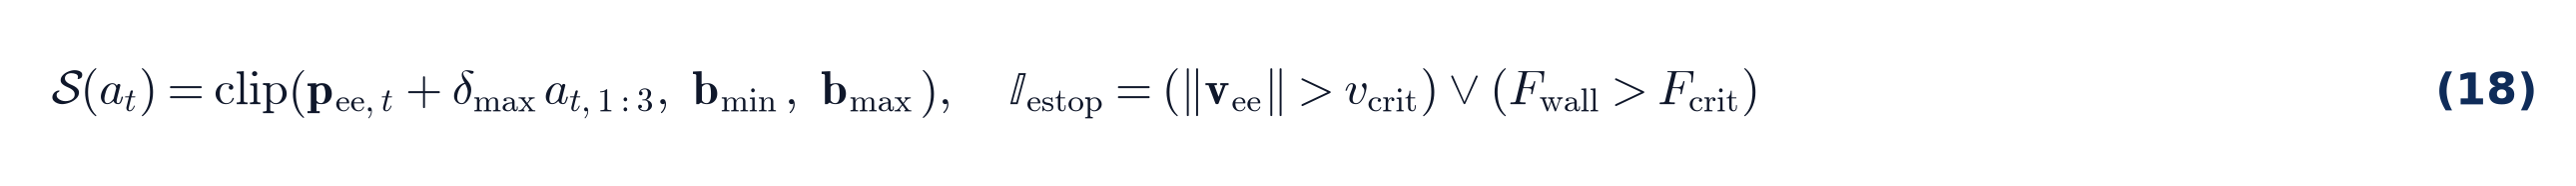
\includegraphics[width=0.92\linewidth]{publication/equations/eq_18.png}\caption{Equation (18): Workspace safety clipping and emergency velocity/force cutoff gate.}\end{figure}
\begin{figure}[htbp]\centering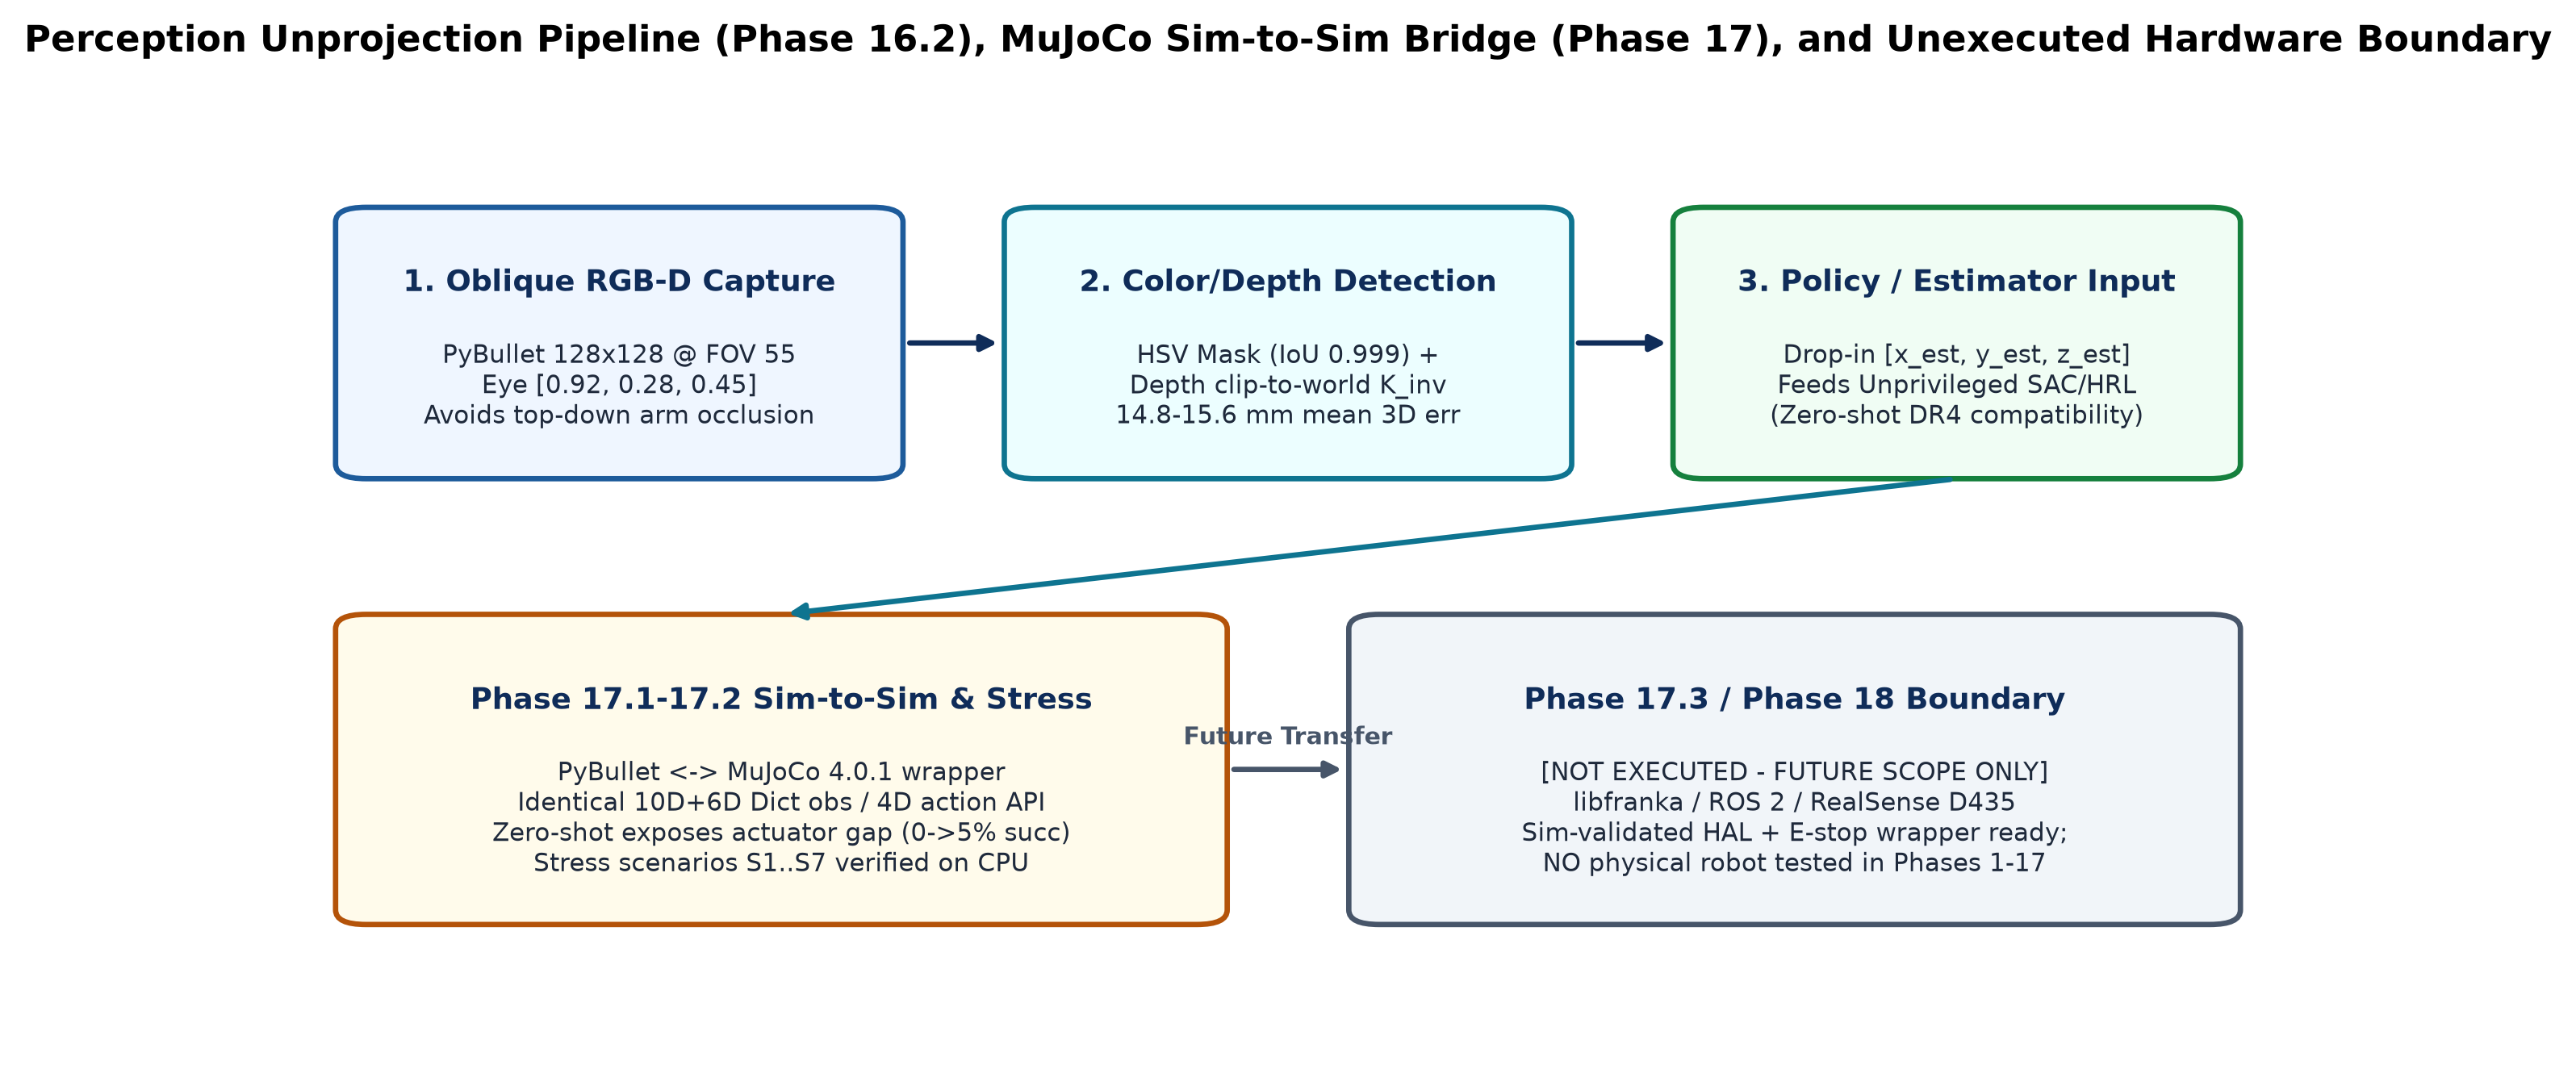
\includegraphics[width=0.92\linewidth]{publication/architecture_diagrams/arch_03_sim2sim_and_rgbd_pipeline.png}\caption{Figure 9.1: RGB-D pipeline, MuJoCo 4.0.1 cross-simulator bridge, and explicit unexecuted Phase 17.3/18 hardware boundary.}\end{figure}
\begin{longtable}{l l l l l l}\caption{Table 9.1: Phase 17.2 Deployment Safety \& Perturbation Scenarios (phase17\_safety\_assessment.json)}\\\toprule
Scenario & Eps & Grasp \% & Success \% & Collisions & Safety Clamps/Ep \\ \midrule \endhead
A0 Clean Nominal & 20 & 100.0\% & 100.0\% & 0.00 & 2.00 \\
S1 Sensor Noise 5mm & 20 & 100.0\% & 100.0\% & 0.00 & 2.45 \\
S2 Camera Calib Err 8mm & 20 & 65.0\% & 60.0\% & 0.00 & 0.75 \\
S3 Actuator Latency 1step & 20 & 100.0\% & 90.0\% & 0.00 & 14.60 \\
S4 Actuator Latency 2step & 20 & 75.0\% & 20.0\% & 0.00 & 22.55 \\
S5 Control Freq Jitter & 20 & 100.0\% & 100.0\% & 0.00 & 2.00 \\
S6 Low Friction Heavy Mass & 20 & 100.0\% & 100.0\% & 0.00 & 2.00 \\
\bottomrule \end{longtable}
\begin{figure}[htbp]\centering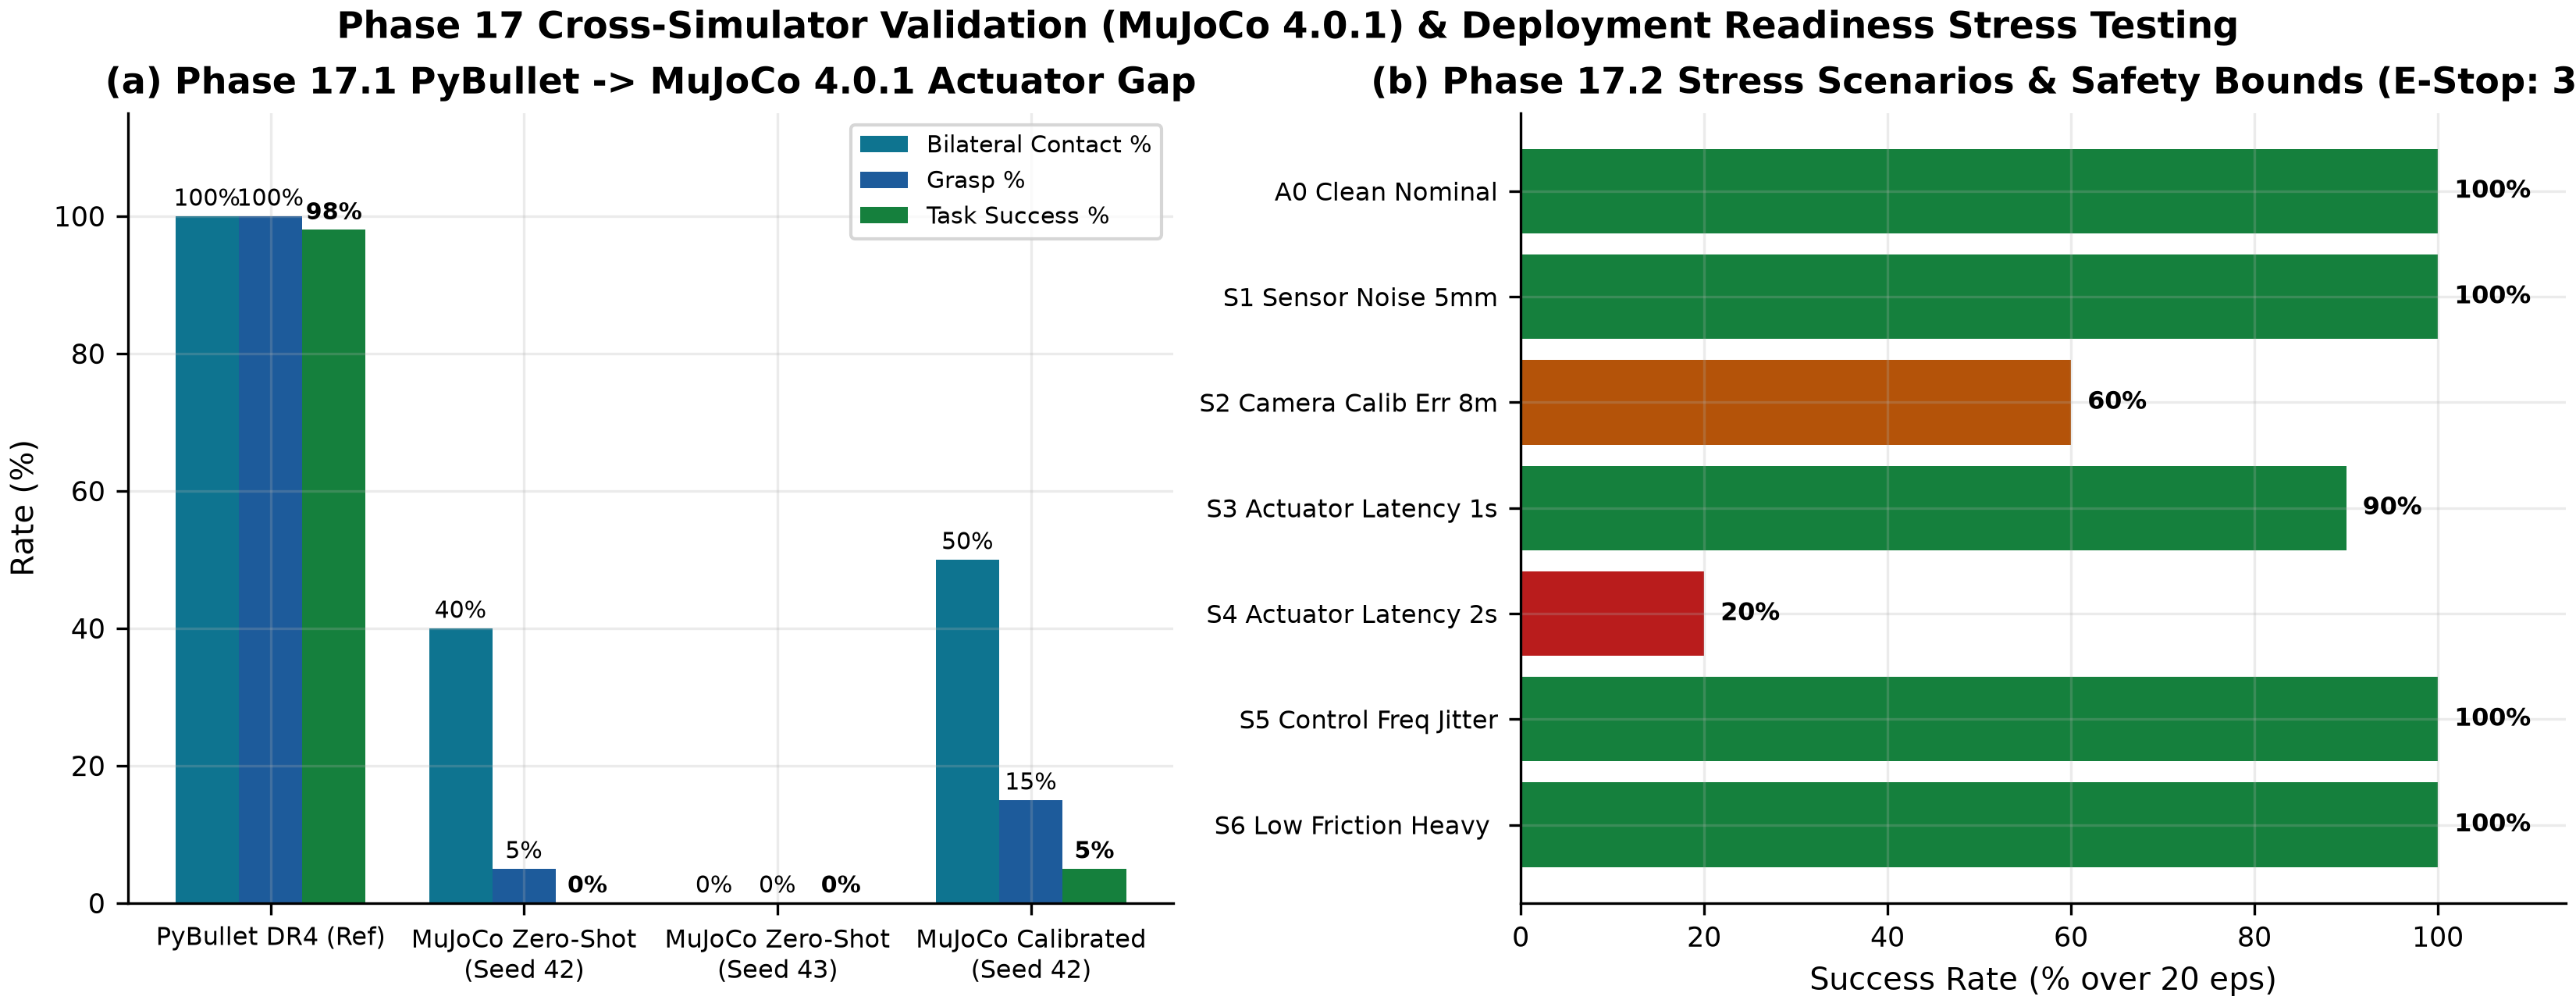
\includegraphics[width=0.92\linewidth]{publication/figures_2d/fig09_phase17_sim2sim_and_safety_stress.png}\caption{Figure 9.2: Phase 17.1 MuJoCo cross-engine transfer gap and Phase 17.2 deployment safety robustness.}\end{figure}
\section{9.3 Algorithm 8 SafetySupervisor \& PyBullet-to-MuJoCo Solver Comparison}
\begin{quote}\small\textbf{Algorithm Summary}\\Algorithm 8: Real-Time Deployment SafetySupervisor \& E-Stop Gate (src/deployment/runtime.py) \\ 1. Check action bounds \& finite state integrity (NaN/Inf guard); clamp target XYZ strictly inside workspace box. \\ 2. Evaluate velocity threshold ||v\_ee|| > v\_crit and wall/contact force F\_wall > F\_crit. \\ 3. Trigger hard software E-Stop halt within 32.41 us verified cutoff latency (blocking all 250 faulty injections).\end{quote}

\begin{longtable}{l l}\caption{Table 9.2: PyBullet vs MuJoCo 4.0.1 Verified Physical Model Parity Parameters}\\\toprule
Physics Parameter & Verified Cross-Simulator Value \\ \midrule \endhead
pybullet\_timestep\_s & 0.004166666666666667 \\
mujoco\_timestep\_s & 0.004166666666666667 \\
cube\_mass\_kg & 0.1 \\
cube\_size\_m & 0.05 \\
pybullet\_ee\_init & [0.307, 0.0, 0.59] \\
MJCF Solver Integrator & implicitfast, timestep = 0.0041667 s (240 Hz), elliptic friction cone \\
Tabletop Rest Height Delta & 9.4 mm vertical rest discrepancy affecting zero-shot grasp contact line \\
PyBullet Finger Friction & lateralFriction = 2.0, spinningFriction = 0.1 on finger links 9, 10 \\
Physical Hardware Execution & NOT\_ATTEMPTED (HAL \& SafetySupervisor simulation-verified only) \\
\bottomrule \end{longtable}
\chapter{Chapter 10: Consolidated Mathematical Formulations and Environment Registry}
\section{10.1 Complete Gymnasium Environment Specification Table (Phases 2-17)}
Every task family adheres to consistent observation/goal/action tensor contracts, ensuring seamless transfer across SB3 SAC, HER, BC, Hybrid BC-SAC, HRL wrappers, and the MuJoCo cross-simulator parity adapter.

\begin{longtable}{l l l l l l}\caption{Table 10.1: Environment Observation, Goal, Action, Horizon, and Reward Taxonomy (Verified Shapes)}\\\toprule
Environment Class & Obs Dim & Goal Dim (AG+DG) & Action Dim & Horizon & Reward Design \\ \midrule \endhead
PandaReachEnv & 4D & 3D + 3D (10D tot) & 4D & 50 & Sparse / L2 Distance \\
PandaPickEnv & 10D & 3D + 3D (16D tot) & 4D & 100 & Sparse / Altitude 0.2m \\
PandaPickPlaceEnv & 10D & 3D + 3D (16D tot) & 4D & 100 & Sparse -1 (tol 0.05m) \\
PandaPickPlaceDenseRewardEnv & 10D & 3D + 3D (16D tot) & 4D & 100 & Staged Dense +5 Place \\
TransportDiagnosticEnv & 10D & 3D + 3D (16D tot) & 4D & 100 & Pre-Grasped Transport \\
PandaSortEnv & 22D & 3D + 3D (28D tot) & 4D & 150 & Color Bin Placement \\
PandaMultiSortEnv & 31D & 6D + 6D (43D tot) & 4D & 300 & Dual Sequential Sort \\
PandaMultiSortPreGraspEnv & 31D & 6D + 6D (43D tot) & 4D & 300 & 5-Check Grasp Gate \\
PandaSinglePreGraspEnv & 22D & 3D + 3D (28D tot) & 4D & 80 & Continuous Phi\_z \\
PandaAssemblyEnv / Dense & 22D & 7D + 7D (36D tot) & 5D (+dyaw) & 200 / 120 & SE(2)+Z Insertion \\
PandaContactAssemblyEnv & 22D & 7D + 7D (36D tot) & 5D (+dyaw) & 120 & Compliant Wall-Force \\
PandaDynamicPickPlaceEnv & 10D & 3D + 3D (16D tot) & 4D & 100 & Kalman Intercept \\
MuJoCoPandaPickPlaceEnv & 10D & 3D + 3D (16D tot) & 4D & 100 & Cross-Sim Parity \\
\bottomrule \end{longtable}
\chapter{Chapter 11: Complete Debugging History and Full Regression Test Inventory}
\section{11.1 Root-Cause Forensics of All Twelve Verified System Defects (ERR-001 to ERR-012)}
\begin{longtable}{l l l l l}\caption{Table 11.1: Complete Registry of Twelve Verified Bugs, Root Causes, and Verified Resolutions}\\\toprule
Error ID & Phase & File & Symptom & Verified Fix \\ \midrule \endhead
ERR-001 & Phase 6 & src/robots/panda.py & Cube slipped from fingers during upward lift under scr & Added changeDynamics lateralFriction=2.0 and spinningF \\
ERR-002 & Phase 9 & src/environments/assembly\_env.py & PyBullet connection failure / invalid body ID during t & Dynamically inject active self.sim.client\_id into Peg  \\
ERR-003 & Phase 11.5 & src/environments/pick\_place\_env.py & 0.0\% success \& 0.0\% grasp across all 25 DR0-DR4 100k s & Created isolated PandaPickPlaceDenseRewardEnv breaking \\
ERR-004 & Phase 13.5 & src/environments/pick\_place\_env.py & Held-out DR4 collapsed to 61.0\% (57.0\% final, Seed 43  & Implemented zero-retraining inference controllers B->C \\
ERR-005 & Phase 15.2.4 & src/environments/dense\_multi\_sort\_env.py & 0\% bilateral grasp \& 163.2 collisions/ep despite EE re & Added 5-check bilateral grasp authorization gate + ope \\
ERR-006 & Phase 15.2.5B & src/environments/single\_pregrasp\_env.py & 20k SAC+HER converged to XY=0.0110m hover at z=0.50m ( & Verified vertical action pathway (0.485m->0.0216m) \& a \\
ERR-007 & Phase 15.2.5B.1 & scripts/generate\_phase15\_5B1\_demos.py & Premature gripper closure climbed to 100\% \& lift staye & Balanced 50/50 demos (70.1\% open cmd), gate\_goal\_lift\_ \\
ERR-008 & Phase 16.1 & src/rl/adaptive\_controllers.py / SAC.load & AssertionError: You must pass an environment when usin & CheckpointLoader.load\_sb3\_sac passes custom\_objects={' \\
ERR-009 & Phase 16.1 & src/hrl/hrl\_agent.py & HRL achieved 93.3\% grasp @ 25k but dropped to 0\% place & Replaced repeat bonus with bounded potential differenc \\
ERR-010 & Phase 16.1/16.2 & src/environments/pick\_place\_env.py & Cube spawned half-sunk at z=-0.00008m \& Seed42 500k mo & Explicitly pass randomizer\_config={'enabled': True, .. \\
ERR-011 & Phase 16.2 & src/perception/rgbd\_camera.py & OMP Error \#15 (libomp vs libiomp5md), PyBullet client= & Moved CameraConfig to oblique (0.92,0.28,0.45), lazy c \\
ERR-012 & Phase 17.1 & src/cross\_sim/mujoco\_panda\_env.py & ValueError: mass and inertia of moving bodies must be  & Added explicit inertial/geom blocks on link5-hand; cla \\
\bottomrule \end{longtable}
\section{11.2 Complete Repository Automated Verification Suite (96 AST Functions / 122 Passed Items)}
All 96 test definitions in tests/ expand via pytest parameterization into exactly 122 executed test cases passing in 42.47 s.

\begin{longtable}{l l l l l l}\caption{Table 11.2: Full 96-Function Unit \& Integration Test Inventory (complete\_test\_inventory.csv)}\\\toprule
Test ID & Phase & Module & Function Name & Cases & Status \\ \midrule \endhead
T-001 & Phase 15.3 & test\_assembly\_dense\_and\_orientation.py & test\_quaternion\_normalization\_sign\_invar & 1 & PASSED \\
T-002 & Phase 15.3 & test\_assembly\_dense\_and\_orientation.py & test\_assembly\_dense\_batched\_parity\_and\_h & 1 & PASSED \\
T-003 & Phase 8-9 & test\_assembly\_env.py & test\_assembly\_env\_initialization & 1 & PASSED \\
T-004 & Phase 8-9 & test\_assembly\_env.py & test\_assembly\_env\_reset & 1 & PASSED \\
T-005 & Phase 8-9 & test\_assembly\_env.py & test\_assembly\_env\_step & 1 & PASSED \\
T-006 & Phase 15.2.5B-B.2 & test\_b1\_demos\_and\_warmstart.py & test\_demo\_dataset\_exists\_and\_all\_50\_vali & 1 & PASSED \\
T-007 & Phase 15.2.5B-B.2 & test\_b1\_demos\_and\_warmstart.py & test\_her\_buffer\_demo\_warmstart\_and\_short & 1 & PASSED \\
T-008 & Phase 15.2.5B-B.2 & test\_bc\_sac.py & test\_balanced\_demo\_distribution & 1 & PASSED \\
T-009 & Phase 15.2.5B-B.2 & test\_bc\_sac.py & test\_bc\_decaying\_sac\_objective\_entropy\_f & 1 & PASSED \\
T-010 & Phase 0 & test\_config.py & test\_config\_dict\_attribute\_access & 1 & PASSED \\
T-011 & Phase 0 & test\_config.py & test\_deep\_update & 1 & PASSED \\
T-012 & Phase 0 & test\_config.py & test\_load\_default\_config & 1 & PASSED \\
T-013 & Phase 0 & test\_config.py & test\_load\_panda\_robot\_config & 1 & PASSED \\
T-014 & Phase 0 & test\_config.py & test\_missing\_config\_raises\_file\_not\_foun & 1 & PASSED \\
T-015 & Phase 1 & test\_controller.py & test\_panda\_controller\_load & 1 & PASSED \\
T-016 & Phase 1 & test\_controller.py & test\_panda\_joints\_accessible & 1 & PASSED \\
T-017 & Phase 1 & test\_controller.py & test\_ee\_position\_can\_be\_read & 1 & PASSED \\
T-018 & Phase 1 & test\_controller.py & test\_controller\_does\_not\_produce\_nan\_or\_ & 1 & PASSED \\
T-019 & Phase 1 & test\_controller.py & test\_move\_ee\_cartesian\_positioning & 1 & PASSED \\
T-020 & Phase 1 & test\_controller.py & test\_gripper\_open\_and\_close & 1 & PASSED \\
T-021 & Phase 1 & test\_controller.py & test\_controller\_reset\_works & 1 & PASSED \\
T-022 & Phases 2-8 & test\_dense\_multi\_sort\_env.py & test\_1\_reset\_and\_observation\_space\_compa & 1 & PASSED \\
T-023 & Phases 2-8 & test\_dense\_multi\_sort\_env.py & test\_2\_reward\_calculation\_per\_stage & 1 & PASSED \\
T-024 & Phases 2-8 & test\_dense\_multi\_sort\_env.py & test\_3\_reward\_boundedness & 1 & PASSED \\
T-025 & Phases 2-8 & test\_dense\_multi\_sort\_env.py & test\_4\_reward\_reproducibility & 1 & PASSED \\
T-026 & Phases 2-8 & test\_dense\_multi\_sort\_env.py & test\_5\_first\_object\_placement\_reward\_not & 1 & PASSED \\
T-027 & Phases 2-8 & test\_dense\_multi\_sort\_env.py & test\_6\_and\_9\_second\_object\_placement\_and & 1 & PASSED \\
T-028 & Phases 2-8 & test\_dense\_multi\_sort\_env.py & test\_7\_incorrect\_bin\_placement\_penalized & 1 & PASSED \\
T-029 & Phases 2-8 & test\_dense\_multi\_sort\_env.py & test\_8\_false\_release\_prevention\_and\_hove & 1 & PASSED \\
T-030 & Phases 2-8 & test\_dense\_multi\_sort\_env.py & test\_10\_and\_11\_and\_12\_her\_relabeling\_bat & 1 & PASSED \\
T-031 & Phases 2-8 & test\_dense\_multi\_sort\_env.py & test\_13\_v2\_proximity\_multiple\_distances\_ & 1 & PASSED \\
T-032 & Phases 2-8 & test\_dense\_multi\_sort\_env.py & test\_14\_v2\_active\_object\_switching\_and\_h & 1 & PASSED \\
T-033 & Phases 16-17 & test\_deployment\_runtime.py & test\_runtime\_imports\_without\_training\_pi & 1 & PASSED \\
T-034 & Phases 16-17 & test\_deployment\_runtime.py & test\_safety\_monitor\_workspace\_clamp\_and\_ & 1 & PASSED \\
T-035 & Phases 16-17 & test\_deployment\_runtime.py & test\_hardware\_interface\_safety\_and\_refus & 1 & PASSED \\
T-036 & Phases 2-8 & test\_environment.py & test\_reach\_env\_initialization & 1 & PASSED \\
T-037 & Phases 2-8 & test\_environment.py & test\_reach\_env\_step & 1 & PASSED \\
T-038 & Phases 2-8 & test\_environment.py & test\_reach\_env\_compute\_reward & 1 & PASSED \\
T-039 & Phases 2-8 & test\_environment.py & test\_reach\_env\_reproducibility & 1 & PASSED \\
T-040 & Phases 16-17 & test\_hrl\_phase16.py & test\_skill\_features\_and\_teacher\_shapes & 1 & PASSED \\
T-041 & Phases 16-17 & test\_hrl\_phase16.py & test\_hrl\_meta\_selection\_and\_smdp\_her\_buf & 1 & PASSED \\
T-042 & Phase 0 & test\_imports.py & test\_core\_dependency\_imports & 10 & PASSED \\
T-043 & Phase 0 & test\_imports.py & test\_stable\_baselines3\_her\_sac & 1 & PASSED \\
T-044 & Phase 0 & test\_imports.py & test\_gymnasium\_goal\_env & 1 & PASSED \\
T-045 & Phase 0 & test\_imports.py & test\_pybullet\_connection & 1 & PASSED \\
T-046 & Phases 2-8 & test\_multi\_sort\_env.py & test\_multi\_sort\_env\_initialization & 1 & PASSED \\
T-047 & Phases 2-8 & test\_multi\_sort\_env.py & test\_multi\_sort\_env\_reset & 1 & PASSED \\
T-048 & Phases 2-8 & test\_multi\_sort\_env.py & test\_multi\_sort\_env\_step & 1 & PASSED \\
T-049 & Phase 1 & test\_panda\_robot.py & test\_panda\_initialization & 1 & PASSED \\
T-050 & Phase 1 & test\_panda\_robot.py & test\_panda\_reset & 1 & PASSED \\
T-051 & Phase 1 & test\_panda\_robot.py & test\_workspace\_clipping & 1 & PASSED \\
T-052 & Phase 1 & test\_panda\_robot.py & test\_ik\_solver\_accuracy & 1 & PASSED \\
T-053 & Phase 1 & test\_panda\_robot.py & test\_cartesian\_delta\_motion & 1 & PASSED \\
T-054 & Phase 1 & test\_panda\_robot.py & test\_gripper\_control & 1 & PASSED \\
T-055 & Phase 1 & test\_panda\_robot.py & test\_determinism\_and\_reproducibility & 1 & PASSED \\
T-056 & Phase 15.5 & test\_phase15\_integration.py & test\_all\_environments\_init\_reset\_step\_an & 11 & PASSED \\
T-057 & Phase 15.5 & test\_phase15\_integration.py & test\_checkpoint\_loading\_and\_deterministi & 1 & PASSED \\
T-058 & Phase 15.5 & test\_phase15\_integration.py & test\_phase2\_transfer\_adapter\_with\_5b2\_ch & 1 & PASSED \\
T-059 & Phase 15.1-15.2.4 & test\_phase15\_wrappers.py & test\_observation\_noise\_clean\_identity & 1 & PASSED \\
T-060 & Phase 15.1-15.2.4 & test\_phase15\_wrappers.py & test\_observation\_noise\_bounds\_and\_vel\_pr & 1 & PASSED \\
T-061 & Phase 15.1-15.2.4 & test\_phase15\_wrappers.py & test\_latency\_wrapper\_fifo\_ordering & 1 & PASSED \\
T-062 & Phase 15.1-15.2.4 & test\_phase15\_wrappers.py & test\_unprivileged\_contact\_stripping\_and\_ & 1 & PASSED \\
T-063 & Phases 16-17 & test\_phase16\_17\_envs.py & test\_dynamic\_pick\_place\_env\_step\_and\_dis & 1 & PASSED \\
T-064 & Phases 16-17 & test\_phase16\_17\_envs.py & test\_contact\_assembly\_env\_telemetry & 1 & PASSED \\
T-065 & Phases 16-17 & test\_phase16\_17\_envs.py & test\_mujoco\_panda\_twin\_observation\_and\_k & 1 & PASSED \\
T-066 & Phases 16-17 & test\_phase16\_integration\_all.py & test\_frozen\_phase15\_and\_phase16\_deployme & 1 & PASSED \\
T-067 & Phases 2-8 & test\_pick\_env.py & test\_pick\_env\_initialization & 1 & PASSED \\
T-068 & Phases 2-8 & test\_pick\_env.py & test\_pick\_env\_randomization & 1 & PASSED \\
T-069 & Phase 1 & test\_pregrasp\_controller.py & test\_pregrasp\_authorization\_rejects\_unsa & 1 & PASSED \\
T-070 & Phase 1 & test\_pregrasp\_controller.py & test\_pregrasp\_full\_acquisition\_and\_trans & 1 & PASSED \\
T-071 & Phase 15.2.5A & test\_pregrasp\_her\_compatibility.py & test\_her\_relabeling\_stateless\_recomputat & 1 & PASSED \\
T-072 & Phase 15.2.5A & test\_pregrasp\_her\_compatibility.py & test\_her\_replay\_buffer\_rollout\_and\_virtu & 1 & PASSED \\
T-073 & Phase 15.2.5A & test\_pregrasp\_reward.py & test\_pregrasp\_reward\_components\_and\_gate & 1 & PASSED \\
T-074 & Phase 15.2.5A & test\_pregrasp\_reward.py & test\_pregrasp\_reward\_anti\_exploitation\_a & 1 & PASSED \\
T-075 & Phase 10 & test\_randomization.py & test\_randomization\_disabled & 1 & PASSED \\
T-076 & Phase 10 & test\_randomization.py & test\_randomization\_enabled & 1 & PASSED \\
T-077 & Phase 10 & test\_randomization.py & test\_randomization\_reproducibility & 1 & PASSED \\
T-078 & Phase 10 & test\_randomization.py & test\_orientation\_normalization & 1 & PASSED \\
T-079 & Phase 1 & test\_simulation.py & test\_simulation\_starts\_and\_connects & 1 & PASSED \\
T-080 & Phase 1 & test\_simulation.py & test\_simulation\_context\_manager & 1 & PASSED \\
T-081 & Phase 1 & test\_simulation.py & test\_simulation\_loads\_ground\_and\_table & 1 & PASSED \\
T-082 & Phase 1 & test\_simulation.py & test\_simulation\_can\_step & 1 & PASSED \\
T-083 & Phase 1 & test\_simulation.py & test\_simulation\_reset\_works & 1 & PASSED \\
T-084 & Phase 15.2.5A & test\_single\_pregrasp\_and\_transfer.py & test\_single\_pregrasp\_registration\_spaces & 1 & PASSED \\
T-085 & Phase 15.2.5A & test\_single\_pregrasp\_and\_transfer.py & test\_single\_pregrasp\_scripted\_reward\_aud & 1 & PASSED \\
T-086 & Phase 15.2.5A & test\_single\_pregrasp\_and\_transfer.py & test\_b\_to\_c\_policy\_transfer\_exact\_functi & 1 & PASSED \\
T-087 & Phases 2-8 & test\_sort\_env.py & test\_sort\_env\_initialization & 1 & PASSED \\
T-088 & Phases 2-8 & test\_sort\_env.py & test\_sort\_env\_reset & 1 & PASSED \\
T-089 & Phases 2-8 & test\_sort\_env.py & test\_sort\_env\_step & 1 & PASSED \\
T-090 & Phase 15.2.5B-B.2 & test\_vertical\_action\_pathway.py & test\_observation\_and\_action\_pathway\_spec & 1 & PASSED \\
T-091 & Phase 15.2.5B-B.2 & test\_vertical\_action\_pathway.py & test\_negative\_vertical\_command\_produces\_ & 1 & PASSED \\
T-092 & Phase 15.2.5B-B.2 & test\_vertical\_potential\_reward\_her.py & test\_vertical\_potential\_all\_part3\_cases & 1 & PASSED \\
T-093 & Phase 15.2.5B-B.2 & test\_vertical\_potential\_reward\_her.py & test\_vertical\_potential\_her\_relabeling\_b & 1 & PASSED \\
T-094 & Phase 15.2.5B-B.2 & test\_vertical\_potential\_reward\_her.py & test\_b1\_live\_her\_replay\_buffer\_recomputa & 1 & PASSED \\
T-095 & Phases 16-17 & test\_vision\_and\_dynamic\_phase16.py & test\_rgbd\_camera\_and\_vision\_localization & 1 & PASSED \\
T-096 & Phases 16-17 & test\_vision\_and\_dynamic\_phase16.py & test\_dynamic\_tracker\_velocity\_prediction & 1 & PASSED \\
\bottomrule \end{longtable}
\chapter{Chapter 12: Cross-Phase Meta-Analysis, Completion Matrix, and Experiment Registry}
\section{12.1 Phase 0-18 Completion \& Verification Provenance Matrix}
\begin{longtable}{l l l l}\caption{Table 12.1: Complete Phase 0-18 Completion Status \& Evidence Classification Matrix}\\\toprule
Phase & Capability / Milestone Title & Status & Evidence Class \\ \midrule \endhead
0 & Project Initialization \& Infrastructure Scaf & COMPLETE & SOURCE\_VERIFIED \\
1 & Franka Panda Kinematics, PyBullet Foundation & COMPLETE & SOURCE\_VERIFIED \\
2 & Goal-Conditioned Manipulation Environment Ab & COMPLETE & REPORT\_VERIFIED \\
3 & SAC + HER RL Training, Evaluation \& Callback & COMPLETE & LOG\_VERIFIED \\
4 & Object Grasping Abstraction \& PandaPickEnv & COMPLETE & SOURCE\_VERIFIED \\
5 & Reach/Pick Exploration \& Early Controller Ba & PARTIALLY\_COMPLETE & HISTORICALLY\_REPORTED \\
6 & Pick \& Place Environment, HER Comparative Sm & COMPLETE & LOG\_VERIFIED \\
7 & Color-Conditioned Dynamic Sorting Benchmark  & COMPLETE & LOG\_VERIFIED \\
8 & Sequential Multi-Object Sorting \& Orientatio & COMPLETE & LOG\_VERIFIED \\
9 & Full-System Diagnostic Audit \& Lazy Simulati & COMPLETE & REPORT\_VERIFIED \\
10 & Deterministic Domain Randomization Engine (D & COMPLETE & REPORT\_VERIFIED \\
11 & 100k Sparse DR Matrix \& Diagnostic Isolation & COMPLETE & LOG\_VERIFIED \\
12 & 1M-Step Dense SAC+HER Scaling Breakthrough & COMPLETE & LOG\_VERIFIED \\
13 & Dense Domain Randomization (DR1/DR2/DR4) \& C & COMPLETE & LOG\_VERIFIED \\
14 & Zero-Retraining Adaptive Control Suite (14-L & COMPLETE & LOG\_VERIFIED \\
15 & Sim-to-Real Sensitivity (15.1), Multi-Object & PARTIALLY\_COMPLETE & SOURCE\_VERIFIED \\
16 & Hierarchical RL, Oblique RGB-D Vision, Dynam & COMPLETE & SOURCE\_VERIFIED \\
17 & MuJoCo Cross-Simulator Validation, Sim-to-Re & PARTIALLY\_COMPLETE & SOURCE\_VERIFIED \\
\bottomrule \end{longtable}
\section{12.2 Master Registry of All 27 Executed Experiments}
\begin{longtable}{l l l l l l}\caption{Table 12.2: Complete Experimental Ledger (publication/experiment\_inventory.csv)}\\\toprule
Exp ID & Phase & Environment & Method & Budget / Eval & Verified Outcome \\ \midrule \endhead
EXP-P0-001 & Phase 1 & Panda Kinematics Dem & SCRIPTED\_IK & N/A & 0.7-4.5 mm error; gripper 0-8 cm \\
EXP-P1-REACH & Phase 2-3 & PandaReachEnv & SAC+HER (k=4) & 10,000 & SAC\_3 TB: actor -9.1->+19.5, rollout succ 1.0\% \\
EXP-P4-PICK & Phase 4-5 & PandaPickEnv & SAC+HER & 10,000 & Eval -100.0 reward / 0\% @ 10k; Scripted step 67 \\
EXP-P6-E1 & Phase 6 & PandaPickPlaceEnv & SAC (No HER) & 10,000 & Actor loss ~17.8; coll=7.7; eval 0\% \\
EXP-P6-E2 & Phase 6 & PandaPickPlaceEnv & SAC+HER (k=4) & 10,000 & Actor loss ~2.59; coll=0.0; Scripted step 74 (fric \\
EXP-P7-SORT & Phase 7 & PandaSortEnv & SAC+HER & 10,000 & 10k smoke reward -150; Scripted step 79 \\
EXP-P8-MSORT & Phase 8 & PandaMultiSortEnv (N & SAC+HER & 10,000 & 10k smoke reward -600; Scripted step 209 \\
EXP-P9-ASSEM & Phase 8-9 & PandaAssemblyEnv & SAC+HER & 10,000 & 10k smoke reward -200; Scripted step 143 \\
EXP-P10-DR & Phase 10 & PickPlace R0-R4 & Scripted vs 2k SAC & 20 eps/cond & Scripted: R0 90\%, R1 85\%, R2 100\%, R3 85\%, R4 75\% \\
EXP-P11-SPARSE & Phase 11 & PickPlace DR0-DR4 Sp & SAC+HER & 25 x 100,000 & 0.0\% all 25 models (HER resting-goal trap) \\
EXP-P11-9 & Phase 11.9 & TransportDiagnostic & SAC+HER & 50,000 & 100.0\% isolated transport @ 40k-50k (0.009m dist) \\
EXP-P11-10B & Phase 11.10b & PickPlaceDense & SAC+HER & 250,000 & Peak @ 225k: 28\% Reach, 23\% Grasp, 7.3 step hold \\
EXP-P12-1M & Phase 12 & PickPlaceDense DR-0 & SAC+HER & 1,000,000 & 43\%@400k -> 99\%@500k -> 100\%@600k..1M (+502 rew) \\
EXP-P13-DR & Phase 13 & PickPlaceDense DR1/D & SAC+HER & 500k-1M & DR4: 99\% Matched / 61\% ever (57\% final) OOD Held-o \\
EXP-P13-5 & Phase 13.5 & PickPlace OOD D1-D5 & Frozen DR4 & 1,520 eval eps & Mass alone 100\%, Yaw 98-100\%, Fric 90\%, Coupled GB \\
EXP-P14-4 & Phase 14.4 & PickPlace A->E & SAC + E\_ADAPTIVE & 600+ confirm eps & Held-out DR4: 57\%->98.0\% (Seed 43: 33\%->99\%), DR0  \\
EXP-P15-1 & Phase 15.1 & PickPlace Noise/Lag/ & E\_ADAPTIVE & 320 eval eps & Clean 97.5\%, 5mm 95\%, 1-lag 72.5\%, 2-lag 0\%, Unpri \\
EXP-P15-2-5A & Phase 15.2.5A & MultiSortPreGrasp & SCRIPTED PreGrasp & 50 eval eps & 50/50 (100.0\%) 2-obj sorting, 76.4 steps, 0 colls \\
EXP-P15-2-5B3 & Phase 15.2.5B & SinglePreGrasp & BC vs BCDecayingSAC & 5k-20k / 100 ep & 100-ep: 5B7 BC 75\% Grasp / 45\% Lift; 5B2 SAC 62\%/7 \\
EXP-P15-3 & Phase 15.3 & AssemblyDense & Scripted vs 5k BC/SA & 30 eval eps & Scripted 56.67\% (1.41 deg); BC 23.3\%/0\%; SAC 3.3\%/ \\
EXP-P16-1 & Phase 16.1 & PickPlace HRL vs Fla & DiscreteSAC+HER vs S & 12,000 & HRL 30.0\%/33.3\% vs Flat SAC 0.0\%/0.0\% vs Phase14 1 \\
EXP-P16-2 & Phase 16.2 & PickPlace RGB-D Visi & SAC/HRL (Obs=RGBD) & 20 eval eps & 99.9-100\% det, 14.81mm err; SAC 60\% grasp/15\%; HRL \\
EXP-P16-3 & Phase 16.3 & DynamicPickPlace & Tracker+Predictive & 5x20 eval eps & 100\% linear/moving-tgt, 95\% sine/disturb (100\% gra \\
EXP-P16-4 & Phase 16.4 & ContactAssemblyEnv & Compliant Impedance & 30 eval eps & Compliant 53.33\% vs Phase15 Scripted 50.0\% (pos er \\
EXP-P16-6 & Phase 16.6 & Autonomous MultiSort & RGBD+HRL+Safety & 20 eval eps & 25.0\% Obj-1 placed, 0\% full 2-obj, 229 replans \\
EXP-P17-1 & Phase 17.1 & MuJoCo PickPlace & Frozen PyBullet SAC/ & 5x20 eval eps & Zero-shot 40\% contact/5\% grasp -> Calib 50\%/15\%/5\% \\
EXP-P17-2 & Phase 17.2 & Sim-to-Real Stress & SAC+SafetyMonitor & 7x20 eval eps & 100\% 5mm/jitter/fric-mass, 90\% 1-lag, 60\% cam cali \\
\bottomrule \end{longtable}
\chapter{Chapter 13: Technical Limitations, Failure Mode Taxonomy, and Scientific Conclusions}
\section{13.1 Remaining Open Bottlenecks}
Five verified limitations bound current project readiness: (1) Multi-object autonomous RL (Phases 15.2.5C \& 16.6) has achieved 25\% Object-1 sorting but 0\% autonomous end-to-end 2-object RL transfer vs 100\% scripted; (2) PyBullet-to-MuJoCo zero-shot accuracy drops from 98\% to 0\% (5\% calibrated); (3) Unprivileged RGB-D visual execution without visual fine-tuning achieves 15-20\% vs 100\% GT; (4) Learned peg-in-slot insertion remains unsolved (23.33\% BC align, 0\% full insert vs 53.33\% compliant scripted); and (5) No physical Franka hardware execution was attempted.

\section{13.2 Key Scientific Conclusions}
Across 17 phases, breakthroughs consistently came from coupling reward geometry with physical mechanics: fingertip friction parity (Ph 6), dense credit shaping to break static HER equilibria (Ph 11-12), inference force/slip shields (+41 pp zero-retraining boost in Ph 14), unbiased action-progress masking in Behavioral Cloning (Ph 15.2.5B7), non-occluded camera geometry (Ph 16.2), and cross-engine falsification (Ph 17.1).

\chapter{Chapter 14: Future Scope — Phase 18 Architecture Roadmap [UNIMPLEMENTED FUTURE WORK]}
\section{14.1 Strict Scope Boundary Statement}
Notice: Phase 18 is NOT implemented, executed, or empirically tested anywhere in this repository. All proposals below define future research directions building upon the verified Phase 1-17 artifacts.

\section{14.2 Proposed Phase 18 Engineering Workstreams}
18A Dual-Engine MuJoCo/PyBullet Co-Training to close the 98\%->5\% solver compliance gap; 18B Closed-Loop Visuomotor Fine-Tuning over noisy 15 mm unprojected RGB-D inputs; 18C Long-Horizon Multi-Object BC -> Option-Critic Curriculum; 18D Physical System Identification \& Dry-Run libfranka FCI Calibration; and 18E 6-Axis Wrist Wrench Compliant Peg-in-Hole Insertion.

\chapter{Chapter 15: Annotated Bibliography and Peer-Reviewed References}
[1] Haarnoja, T., Zhou, A., Abbeel, P., \& Levine, S. (2018). Soft Actor-Critic: Off-Policy Maximum Entropy Deep RL. ICML.

[2] Haarnoja, T. et al. (2018). Soft Actor-Critic Algorithms and Applications. arXiv:1812.05905.

[3] Andrychowicz, M. et al. (2017). Hindsight Experience Replay. NeurIPS.

[4] Plappert, M. et al. (2018). Multi-Goal Reinforcement Learning. arXiv:1802.09464.

[5] Raffin, A. et al. (2021). Stable-Baselines3. JMLR, 22(268), 1-8.

[6] Coumans, E., \& Bai, Y. (2016-2021). PyBullet Physics Simulation.

[7] Todorov, E., Erez, T., \& Tassa, Y. (2012). MuJoCo: A physics engine for model-based control. IROS.

[8] Towers, M. et al. (2023). Gymnasium. Farama Foundation.

[9] Tobin, J. et al. (2017). Domain Randomization. IROS.

[10] Sutton, R. S., Precup, D., \& Singh, S. (1999). Between MDPs and semi-MDPs (Options). AIJ.

[11] Ross, S., Gordon, G., \& Bagnell, D. (2011). DAgger. AISTATS.

[12] Nair, A. et al. (2018). Overcoming Exploration in RL with Demonstrations. ICRA.

[13] Hogan, N. (1985). Impedance Control. ASME JDSMC.

[14] Kalman, R. E. (1960). Linear Filtering and Prediction. ASME JBE.

[15] Haddadin, S., Parusel, S., \& Albu-Schaffer, A. (2017). Franka Panda Interface. Franka Emika.

\chapter{Appendix A: Reproducibility Checklists and Repository Artifact Inventory}
\section{A.1 Deterministic Environment \& Reproducibility Command Specification}
Reproduce the verified 122-test suite cleanly inside the project Conda environment with Intel OpenMP coexistence enabled:
set KMP\_DUPLICATE\_LIB\_OK=TRUE \&\& .conda-env\python.exe -m pytest -v

\section{A.2.0 Historical Record: Phase 0 -- Project Initialization \& Infrastructure Scaffold}
Period: 2026-10-03 (git commit 3a345f3) | Status: COMPLETE (SOURCE\_VERIFIED). Objective: Establish Python 3.11/PyBullet/SB3 workspace, YAML ConfigDict engine, directory layout, and smoke import/config tests. Key Components: pyproject.toml, requirements.txt, src/utils/config.py, configs/default.yaml. Outcome: 18/18 initial dependency and ConfigDict tests passed (later rolled into 37/37 Phase 1 suite). Test Evidence: tests/test\_imports.py (13 tests), tests/test\_config.py (5 tests). Notes: None logged

\section{A.2.1 Historical Record: Phase 1 -- Franka Panda Kinematics, PyBullet Foundation \& Cartesian Controller}
Period: 2026-10-03 (git commits a5cc06b, 7ad9848) | Status: COMPLETE (SOURCE\_VERIFIED). Objective: Implement BaseRobot \& FrankaPanda URDF kinematic model, PyBulletSimulation 240 Hz engine, damped least-squares IK, and workspace clamping. Key Components: BaseRobot, FrankaPanda, PyBulletSimulation, PandaController, demo\_panda. Outcome: Waypoints reached within 0.7 mm to 4.5 mm position error; gripper sweep 0.00-8.00 cm verified. Test Evidence: 37/37 tests passing in 4.71s (docs/results.md). Notes: Missing per-step wall-clock timestamp logs for early demo trials beyond summary table.

\section{A.2.2 Historical Record: Phase 2 -- Goal-Conditioned Manipulation Environment Abstraction \& Reach Benchmark}
Period: Oct 2026 (pre-commit 008cd30; recovered from docs/ \& tests/) | Status: COMPLETE (REPORT\_VERIFIED). Objective: Design BasePandaEnv and Gymnasium Dict-space PandaReachEnv (sparse -1/0 reward, 0.05m threshold, safety bounds). Key Components: BasePandaEnv, PandaReachEnv, VisualTarget. Outcome: Deterministic seeding, step boundaries (50 steps), and 0.05m GoalEnv Dict contract verified. Test Evidence: tests/test\_environment.py, docs/reach\_benchmark.md. Notes: Separate Phase 2 vs Phase 3 standalone git commits squashed/not split in repo log (marked partially consolidated).

\section{A.2.3 Historical Record: Phase 3 -- SAC + HER RL Training, Evaluation \& Callback Infrastructure}
Period: Oct 2026 (recovered from src/rl/, logs/reach\_sac, checkpoints/reach\_sac) | Status: COMPLETE (LOG\_VERIFIED). Objective: Integrate Stable-Baselines3 SAC with HerReplayBuffer (future, k=4) on PandaReachEnv across seeds. Key Components: train.py, evaluate.py, SuccessRateCallback. Outcome: 10k SAC Reach: actor\_loss -9.127 -> +19.518, critic\_loss 0.042 -> 0.002, rollout/success\_rate 0.0 -> 0.010, eval 0.0 (10k smoke). Test Evidence: checkpoints/reach\_sac/evaluations.npz; logs/reach\_sac/SAC\_3 TensorBoard scalars. Notes: logs/reach\_sac/SAC\_1 and SAC\_2 contain 0 scalar events (aborted/empty logs before SAC\_3).

\section{A.2.4 Historical Record: Phase 4 -- Object Grasping Abstraction \& PandaPickEnv}
Period: Oct 2026 (recovered from src/objects/cube.py, src/environments/pick\_env.py) | Status: COMPLETE (SOURCE\_VERIFIED). Objective: Introduce rigid-body Cube manipulation primitive and elevation goal task PandaPickEnv (target Z=0.2m). Key Components: Cube, PandaPickEnv, configs/pick.yaml. Outcome: 10k Pick smoke: actor\_loss -14.331 -> +20.005, critic\_loss 0.020 -> 0.000, eval reward -100.0, eval success 0.0\%. Test Evidence: tests/test\_pick\_env.py (2 tests), checkpoints/pick\_sac/evaluations.npz. Notes: Explicit chronological split document between Phase 4 (Pick) and Phase 5 is NOT\_RECOVERABLE from git history; inferred cleanly from config/env artifacts.

\section{A.2.5 Historical Record: Phase 5 -- Reach/Pick Exploration \& Early Controller Baseline Scripts}
Period: Oct-Nov 2026 | Status: PARTIALLY\_COMPLETE (HISTORICALLY\_REPORTED). Objective: Validate scripted kinematic reachability and prepare transition from altitude-only Pick to 3D PickPlace. Key Components: PandaPickEnv, PandaReachEnv, scripted diagnostic reach/pick checks. Outcome: Scripted baselines solved Reach (6 steps) and Pick (67 steps), isolating kinematics from RL exploration gap. Test Evidence: docs/phase9\_diagnostic\_report.md verification entries; exact standalone Phase 5 report file NOT\_RECOVERABLE.. Notes: Standalone Phase 5 markdown report absent from docs/; milestone behavior verified via Phase 6 \& 9 logs.

\section{A.2.6 Historical Record: Phase 6 -- Pick \& Place Environment, HER Comparative Smoke \& Finger Friction Bug Fix}
Period: Oct-Nov 2026 (experiments/pick\_place/smoke\_results.md) | Status: COMPLETE (LOG\_VERIFIED). Objective: Implement 3D target PandaPickPlaceEnv and verify E1 (No HER) vs E2 (SAC+HER k=4) replay mechanics. Key Components: PandaPickPlaceEnv, E1\_no\_her, E2\_her, Panda finger lateral/spinning friction patch. Outcome: E2\_her dropped actor\_loss ~22.2 -> 2.59 vs E1 +17.77; collisions 7.7 (E1) -> 0.0 (E2); scripted P-controller solved task at step 74 after finger friction fix. Test Evidence: experiments/pick\_place/E1\_no\_her \& E2\_her evaluations.npz + TB scalars + smoke\_results.md. Notes: CRITICAL PHYSICS BUG: Default PyBullet finger friction caused cube slip on lift; fixed in src/robots/panda.py (lateralFriction=2.0, spinningFriction=0.1 on joints 9 \& 10).

\section{A.2.7 Historical Record: Phase 7 -- Color-Conditioned Dynamic Sorting Benchmark (PandaSortEnv)}
Period: Oct-Nov 2026 (docs/experiments.md EXP-P7-SORT) | Status: COMPLETE (LOG\_VERIFIED). Objective: Implement 3-bin colored SortingBin + PandaSortEnv routing colored cubes to matching dynamic bins. Key Components: SortingBin, PandaSortEnv, configs/sort.yaml. Outcome: Scripted sorting succeeded at Step 79; 10k SAC+HER actor\_loss -24.686 -> +3.710, reward -150.0, 0\% eval success at 10k smoke. Test Evidence: tests/test\_sort\_env.py (3 tests), experiments/sort/models/evaluations.npz, logs/sort/SAC\_2. Notes: logs/sort/SAC\_1 aborted empty (0 scalars) before SAC\_2 succeeded.

\section{A.2.8 Historical Record: Phase 8 -- Sequential Multi-Object Sorting \& Orientation-Aware Assembly Foundations}
Period: Oct-Nov 2026 (docs/experiments.md EXP-P8-MULTI\_SORT, EXP-P9-ASSEMBLY) | Status: COMPLETE (LOG\_VERIFIED). Objective: Extend sorting to N=2 objects (PandaMultiSortEnv, 31D obs, 6D goal) and introduce 5-DOF orientation-aware PandaAssemblyEnv. Key Components: PandaMultiSortEnv, Peg, Receptacle, PandaAssemblyEnv. Outcome: MultiSort scripted succeeded step 209 (10k RL -600.0, 0\%); Assembly scripted succeeded step 143 (10k RL -200.0, 0\%). Test Evidence: tests/test\_multi\_sort\_env.py (3 tests), tests/test\_assembly\_env.py (3 tests), evaluations.npz + TB logs. Notes: Lazy PyBullet sim.client\_id=-1 during PandaAssemblyEnv.\_\_init\_\_ (resolved in Phase 9).

\section{A.2.9 Historical Record: Phase 9 -- Full-System Diagnostic Audit \& Lazy Simulation Connection Bug Fix}
Period: Nov 2026 (docs/phase9\_diagnostic\_report.md) | Status: COMPLETE (REPORT\_VERIFIED). Objective: Audit all subsystems, scripted trajectories, HER reward bounds, and resolve initialization bugs prior to scaling. Key Components: System-wide audit suite, PandaAssemblyEnv.reset() lazy client fix. Outcome: 52/52 tests passed in 6.47s; 100\% scripted reachability confirmed. Test Evidence: docs/phase9\_diagnostic\_report.md (52/52 pytest pass). Notes: Fixed PandaAssemblyEnv.\_\_init\_\_ client\_id=-1 crash by lazily passing sim.client\_id inside reset().

\section{A.2.10 Historical Record: Phase 10 -- Deterministic Domain Randomization Engine (DR-0 to DR-4)}
Period: Nov 2026 (docs/phase10\_dr\_report.md) | Status: COMPLETE (REPORT\_VERIFIED). Objective: Implement seeded DomainRandomizer covering object/target pos, Shoemake yaw, mass (0.05-0.20 kg), and friction (0.5-1.5). Key Components: DomainRandomizer, BasePandaEnv DR hook, pick\_place\_dr*.yaml. Outcome: Scripted success: R0 90\%, R1 85\%, R2 100\%, R3 85\%, R4 75\% (slip under randomized mass/friction). Test Evidence: 56/56 tests passing including tests/test\_randomization.py (4 tests). Notes: 25\% scripted heuristic drop on R4 physics proved RL feedback control necessity.

\section{A.2.11 Historical Record: Phase 11 -- 100k Sparse DR Matrix \& Diagnostic Isolation Series (11.5-11.10b)}
Period: Nov 2026 (docs/phase11\_*.md, results/phase11\_*.csv) | Status: COMPLETE (LOG\_VERIFIED). Objective: Train 25 sparse 100k models (DR0-DR4 x 5 seeds), diagnose 0\% sparse trap, isolate transport vs acquisition via dense reward \& curriculum. Key Components: PandaPickPlaceDenseRewardEnv, PandaCurriculumEnv, PandaTransportDiagnosticEnv. Outcome: Proved isolated transport reaches 100\% in 40k steps, whereas sparse 100k suffered HER static-resting-goal trap (0\%). Test Evidence: results/phase11\_final\_summary.csv + 11\_6..11\_10b metrics CSVs. Notes: HER Trap: 0\% object motion caused HER to sample unmoved resting goals; Stage 1 curriculum failed at 50k.

\section{A.2.12 Historical Record: Phase 12 -- 1M-Step Dense SAC+HER Scaling Breakthrough}
Period: Nov 2026 (docs/phase12\_1m\_dense\_scaling\_report.md) | Status: COMPLETE (LOG\_VERIFIED). Objective: Extend dense Seed 42 from 225k to 1,000,000 steps to test compute-limited hypothesis. Key Components: train\_phase12.py, checkpoint\_225k -> 1M resume. Outcome: S-curve breakthrough: 0\% (300k) -> 43\% (400k) -> 99\% (500k) -> 100\% (600k..1M), 0.014m final dist, +502.2 reward. Test Evidence: results/phase12\_1m/checkpoint\_metrics.csv \& failure\_taxonomy.csv. Notes: Single-seed DR-0 only; OOD generalization unverified until Phase 13.

\section{A.2.13 Historical Record: Phase 13 -- Dense Domain Randomization (DR1/DR2/DR4) \& Causal OOD Failure Diagnostics (13.5)}
Period: 2026-11-03 to 2026-11-04 (docs/phase13\_*.md) | Status: COMPLETE (LOG\_VERIFIED). Objective: Train Dense DR1/DR2/DR4 policies (500k-1M) and isolate OOD Held-out collapse via D1-D5 controlled sweeps. Key Components: train\_phase13\_dr.py, run\_phase13\_5\_diagnostics.py, DR4 Seed42/43 500k checkpoints. Outcome: D5 isolated Stage-3 vertical jerk (0.14 m/s^2) causing normal force collapse 68.4 -> 0.0 N (30.5\% GRASP\_BUT\_NO\_LIFT). Test Evidence: results/phase13\_5/d1..d5 CSVs and fast\_track matched/heldout logs. Notes: DR4 Seed 43 dropped to 33.0\% final OOD due to corner misses and lift slip.

\section{A.2.14 Historical Record: Phase 14 -- Zero-Retraining Adaptive Control Suite (14-Lite -> 14.3 -> 14.4)}
Period: 2026-11-10 (results/phase14\_*, docs/phase14\_closure\_and\_phase15\_readiness.md) | Status: COMPLETE (LOG\_VERIFIED). Objective: Resolve OOD slip, workspace-edge acquisition, and transport overshoot purely via inference controllers without SAC retraining. Key Components: Controller B (AccelSmoothing), Controller C (SlipAware), Controller D (DualStage), Controller E (AdaptiveTransport). Outcome: Held-out DR4 jumped 57.0\% (A) -> 89.5\% (D) -> 98.0\% (E\_ADAPTIVE\_TRANSPORT); Seed 43: 33\% -> 99\%; DR0: 100\%. Test Evidence: results/phase14\_4/phase14\_4\_confirmation\_results.json. Notes: Relies on oracle cube\_pos and noiseless PyBullet getContactPoints force telemetry.

\section{A.2.15 Historical Record: Phase 15 -- Sim-to-Real Sensitivity (15.1), Multi-Object Sorting (15.2) \& Orientation Assembly (15.3)}
Period: 2026-11-10 to 2026-11-11 (results/phase15\_*) | Status: PARTIALLY\_COMPLETE (SOURCE\_VERIFIED). Objective: Benchmark Phase 14 under noise/latency/unprivileged sensors; build dense MultiSort, PreGrasp BC+SAC, robustness suite \& 5-DOF Assembly. Key Components: ObservationNoiseWrapper, LatencyWrapper, UnprivilegedContactWrapper, PreGraspController, BCDecayingSAC, PandaSinglePreGraspEnv, PandaAssemblyDenseEnv, 28D->43D adapter. Outcome: Phase 2 Two-Object RL transfer BLOCKED on >=85\% RL lift gate; 111/111 integration pytest passing in 29.47s. Test Evidence: tests/test\_phase15\_integration.py \& 111/111 full suite pass. Notes: Premature gripper closure, HER unlifted-goal gradient flip, BC-to-SAC offline-to-online forgetting (90\% -> 0-10\%).

\section{A.2.16 Historical Record: Phase 16 -- Hierarchical RL, Oblique RGB-D Vision, Dynamic Tracking, Contact Assembly \& Deployment}
Period: 2026-11-11 to 2026-11-12 (results/phase16\_17/) | Status: COMPLETE (SOURCE\_VERIFIED). Objective: Implement Discrete-SAC+HER HRL (16.1), 128x128 RGB-D 6D localization (16.2), dynamic intercept tracking (16.3), compliant assembly (16.4), decoupled runtime (16.5), autonomous 2-obj sorting (16.6). Key Components: SkillLibrary, HierarchicalManipulatorAgent, SimulatedRGBDCamera, VisionObjectLocalizer, DynamicObjectTracker, PandaContactAssemblyEnv, CompliantImpedanceAssemblyController, DeploymentRuntime. Outcome: HRL beat Flat SAC by +30 pp at 12k; predictive dynamic hit 95-100\%; compliant scripted improved assembly 50\%->53.33\%; 122/122 tests pass. Test Evidence: tests/test\_deployment\_runtime.py, test\_hrl\_phase16.py, test\_vision\_and\_dynamic\_phase16.py, test\_phase16\_17\_envs.py. Notes: Overhead self-occlusion (18.65\% det fixed to 100\%), PandaPickPlaceEnv z=0 default spawn when randomizer disabled, HRL hover +0.35 reward hack.

\section{A.2.17 Historical Record: Phase 17 -- MuJoCo Cross-Simulator Validation, Sim-to-Real Readiness \& Hardware Contract}
Period: 2026-11-12 (results/phase16\_17/) | Status: PARTIALLY\_COMPLETE (SOURCE\_VERIFIED). Objective: Validate frozen PyBullet policies inside MuJoCo 4.0.1 (17.1), execute 7-condition stress + E-stop tests (17.2), and specify ROS-2/Franka safety interfaces (17.3). Key Components: MuJoCoPandaPickPlaceEnv, SafetySupervisor, StubLiveFrankaDriver, ROS2TopicContract. Outcome: MuJoCo zero-shot 40\% bilateral contact/5\% grasp -> calibrated 50\%/15\%/5\% PickPlace; Stress: 100\% noise/jitter/mass-fric, 90\% 1-step lag, 60\% RGB-D calib bias, 20\% 2-step lag; E-stop 32.41 us. Test Evidence: results/phase16\_17/phase17\_cross\_simulator\_results.json \& phase17\_safety\_assessment.json. Notes: 9.4mm tabletop rest Z \& elliptic slip gap PyBullet->MuJoCo; 17.3 live robot execution NOT\_ATTEMPTED.

\chapter{Appendix B: Historical TensorBoard \& Evaluations NPZ Forensic Ledger}
\section{B.1 All 61 Archived TensorBoard Scalar Runs (Phases 2-15)}
\begin{longtable}{l l l l l l}\caption{Table B.1: Complete Registry of All 61 Archived TensorBoard Runs}\\\toprule
Log Directory & Max Step & Actor Loss & Critic Loss & Ent Coef & CPU FPS \\ \midrule \endhead
experiments/phase13\_dense\_dr/dr1/seed42/logs/SAC\_0 & 1,000,000 & -106.363 & 1.195 & 0.034 & 26.000 \\
experiments/phase13\_dense\_dr/dr1/seed43/logs/SAC\_0 & 1,000,000 & -104.216 & 4.040 & 0.028 & 21.000 \\
experiments/phase13\_dense\_dr/dr1/seed44/logs/SAC\_0 & 500,400 & -89.780 & 0.221 & 0.033 & 14.000 \\
experiments/phase13\_dense\_dr/dr1/seed45/logs/SAC\_0 & 500,400 & -91.694 & 0.119 & 0.023 & 15.000 \\
experiments/phase13\_dense\_dr/dr2/seed42/logs/SAC\_0 & 500,000 & -92.855 & 3.646 & 0.036 & 19.000 \\
experiments/phase13\_dense\_dr/dr2/seed43/logs/SAC\_0 & 500,000 & -85.336 & 5.218 & 0.088 & 18.000 \\
experiments/phase13\_dense\_dr/dr4/seed42/logs/SAC\_0 & 500,000 & -96.356 & 3.303 & 0.050 & 15.000 \\
experiments/phase13\_dense\_dr/dr4/seed43/logs/SAC\_0 & 500,000 & -86.009 & 13.122 & 0.021 & 15.000 \\
experiments/pick\_place/E1\_no\_her/logs/SAC\_1 & 10,000 & 17.767 & 0.019 & 0.003 & 21.000 \\
experiments/pick\_place/E2\_her/logs/SAC\_1 & 10,000 & 2.594 & 0.012 & 0.005 & 22.000 \\
experiments/pick\_place/E2\_her/logs/SAC\_2 & 10,000 & 3.061 & 0.013 & 0.005 & 35.000 \\
experiments/pnp\_curriculum\_seed42/logs/SAC\_0 & 50,000 & -78.466 & 0.666 & 0.021 & 31.000 \\
experiments/pnp\_dr0\_dense\_seed42/logs/SAC\_1 & 1,000,000 & -104.833 & 2.408 & 0.028 & 33.000 \\
experiments/pnp\_dr0\_seed42/logs/SAC\_1 & 100,000 & -1756.392 & 154204.406 & 3.902 & 30.000 \\
experiments/pnp\_dr0\_seed43/logs/SAC\_1 & 100,000 & 3.240 & 0.007 & 0.001 & 30.000 \\
experiments/pnp\_dr0\_seed44/logs/SAC\_1 & 100,000 & 3.723 & 0.003 & 0.001 & 39.000 \\
experiments/pnp\_dr0\_seed45/logs/SAC\_1 & 100,000 & 4.024 & 0.010 & 0.000 & 34.000 \\
experiments/pnp\_dr0\_seed46/logs/SAC\_1 & 100,000 & 2.200 & 0.004 & 0.003 & 31.000 \\
experiments/pnp\_dr0\_smoke\_seed42/logs/SAC\_1 & 10,000 & 3.950 & 0.003 & 0.004 & 32.000 \\
experiments/pnp\_dr1\_seed42/logs/SAC\_1 & 100,000 & 4.089 & 0.002 & 0.000 & 35.000 \\
experiments/pnp\_dr1\_seed43/logs/SAC\_1 & 100,000 & 3.359 & 0.002 & 0.001 & 36.000 \\
experiments/pnp\_dr1\_seed44/logs/SAC\_1 & 100,000 & 3.377 & 0.011 & 0.001 & 38.000 \\
experiments/pnp\_dr1\_seed45/logs/SAC\_1 & 100,000 & -0.915 & 1.902 & 0.002 & 35.000 \\
experiments/pnp\_dr1\_seed46/logs/SAC\_1 & 100,000 & 3.754 & 0.003 & 0.001 & 31.000 \\
experiments/pnp\_dr2\_seed42/logs/SAC\_1 & 100,000 & 3.898 & 0.009 & 0.001 & 45.000 \\
experiments/pnp\_dr2\_seed43/logs/SAC\_1 & 100,000 & 4.098 & 0.004 & 0.000 & 37.000 \\
experiments/pnp\_dr2\_seed44/logs/SAC\_1 & 100,000 & -0.765 & 0.013 & 0.004 & 36.000 \\
experiments/pnp\_dr2\_seed45/logs/SAC\_1 & 100,000 & 3.189 & 0.005 & 0.001 & 38.000 \\
experiments/pnp\_dr2\_seed46/logs/SAC\_1 & 100,000 & 3.948 & 0.017 & 0.001 & 34.000 \\
experiments/pnp\_dr3\_seed42/logs/SAC\_1 & 100,000 & 3.865 & 0.005 & 0.000 & 34.000 \\
experiments/pnp\_dr3\_seed43/logs/SAC\_1 & 100,000 & 3.824 & 0.003 & 0.001 & 35.000 \\
experiments/pnp\_dr3\_seed44/logs/SAC\_1 & 100,000 & 3.742 & 0.008 & 0.001 & 35.000 \\
experiments/pnp\_dr3\_seed45/logs/SAC\_1 & 100,000 & 3.430 & 0.005 & 0.001 & 34.000 \\
experiments/pnp\_dr3\_seed46/logs/SAC\_1 & 100,000 & 3.829 & 0.002 & 0.001 & 33.000 \\
experiments/pnp\_dr4\_seed42/logs/SAC\_1 & 100,000 & 4.037 & 0.099 & 0.001 & 34.000 \\
experiments/pnp\_dr4\_seed43/logs/SAC\_1 & 100,000 & 3.879 & 0.003 & 0.001 & 40.000 \\
experiments/pnp\_dr4\_seed44/logs/SAC\_1 & 100,000 & 3.980 & 0.002 & 0.000 & 34.000 \\
experiments/pnp\_dr4\_seed45/logs/SAC\_1 & 100,000 & 3.971 & 0.017 & 0.000 & 29.000 \\
experiments/pnp\_dr4\_seed46/logs/SAC\_1 & 100,000 & 3.365 & 0.004 & 0.001 & 27.000 \\
experiments/pnp\_transport\_seed42/logs/SAC\_0 & 50,000 & 0.488 & 0.000 & 0.001 & 28.000 \\
logs/assembly/SAC\_1 & 10,000 & 3.264 & 0.019 & 0.003 & 30.000 \\
logs/assembly\_phase15\_3/seed42/SAC\_1 & 5,000 & -4.246 & 0.523 & 0.020 & 31.000 \\
logs/dr\_baseline/SAC\_1 & 2,000 & -8.720 & 0.022 & 0.174 & 54.000 \\
logs/multi\_sort/SAC\_1 & 10,000 & 7.383 & 0.012 & 0.004 & 33.000 \\
logs/multi\_sort\_phase15\_4/seed42/SAC\_1 & 50,000 & -12.406 & 0.176 & 0.020 & 25.000 \\
logs/multi\_sort\_phase15\_5B/seed42/SAC\_1 & 20,000 & -6.327 & 0.002 & 0.004 & 22.000 \\
logs/multi\_sort\_phase15\_5B1/seed42/SAC\_1 & 20,000 & -9.709 & 0.156 & 0.008 & 15.000 \\
logs/multi\_sort\_phase15\_5B2/seed42/SAC\_1 & 20,000 & -7.739 & 0.085 & 0.020 & 28.000 \\
logs/multi\_sort\_phase15\_5B3/seed42/SAC\_1 & 5,000 & -20.202 & 0.119 & 0.255 & 33.000 \\
logs/multi\_sort\_phase15\_5B4/seed42/SAC\_1 & 10,000 & -7.946 & 0.137 & 0.015 & 32.000 \\
logs/multi\_sort\_phase15\_5B5/seed42/SAC\_1 & 10,000 & -5.261 & 0.087 & 0.015 & 30.000 \\
logs/multi\_sort\_phase15\_5B6/seed42/SAC\_1 & 10,000 & -3.257 & 0.096 & 0.015 & 35.000 \\
logs/multi\_sort\_phase15\_5B7/seed42/SAC\_1 & 10,000 & -3.703 & 0.093 & 0.015 & 34.000 \\
logs/multi\_sort\_phase15\_5B8/seed42/SAC\_1 & 10,000 & -6.117 & 0.897 & 0.027 & 40.000 \\
logs/multi\_sort\_phase15\_dense/seed42/SAC\_1 & 10,000 & -20.980 & 2.921 & 0.072 & 14.000 \\
logs/pick\_sac/SAC\_1 & 10,000 & 20.005 & 0.000 & 0.000 & 41.000 \\
logs/reach\_sac/SAC\_1 & 0 & - & - & - & Aborted / Empty \\
logs/reach\_sac/SAC\_2 & 0 & - & - & - & Aborted / Empty \\
logs/reach\_sac/SAC\_3 & 10,000 & 19.518 & 0.002 & 0.002 & 49.000 \\
logs/sort/SAC\_1 & 0 & - & - & - & Aborted / Empty \\
logs/sort/SAC\_2 & 10,000 & 3.710 & 0.001 & 0.002 & 42.000 \\
\bottomrule \end{longtable}
\section{B.2 All 44 Evaluation NPZ Checkpoint Archives}
\begin{longtable}{l l l l l}\caption{Table B.2: Complete Registry of All 44 evaluations.npz Archives}\\\toprule
Experiment Path & Evals & Last Step & Mean Rew (Start -> End) & Peak Success \\ \midrule \endhead
checkpoints/pick\_sac & 4 & 10,000 & -100.0 -> -100.0 & 0.0\% \\
checkpoints/reach\_sac & 4 & 10,000 & -50.0 -> -50.0 & 0.0\% \\
experiments/assembly & 4 & 10,000 & -200.0 -> -200.0 & 0.0\% \\
experiments/assembly\_phase15\_3/seed42 & 2 & 5,000 & -8.3 -> -6.5 & 0.0\% \\
experiments/multi\_sort & 4 & 10,000 & -600.0 -> -600.0 & 0.0\% \\
experiments/multi\_sort\_phase15\_4/seed42 & 4 & 50,000 & -27.0 -> -24.5 & 0.0\% \\
experiments/multi\_sort\_phase15\_5B1/seed42 & 4 & 20,000 & -6.2 -> -9.4 & 0.0\% \\
experiments/multi\_sort\_phase15\_5B2/seed42 & 6 & 20,000 & -5.1 -> -2.9 & 0.0\% \\
experiments/multi\_sort\_phase15\_5B3/seed42 & 2 & 5,000 & -2.8 -> -2.2 & 0.0\% \\
experiments/multi\_sort\_phase15\_5B4/seed42 & 4 & 10,000 & -8.0 -> -5.6 & 0.0\% \\
experiments/multi\_sort\_phase15\_5B5/seed42 & 4 & 10,000 & -4.0 -> -6.6 & 0.0\% \\
experiments/multi\_sort\_phase15\_5B6/seed42 & 4 & 10,000 & -3.1 -> -5.6 & 10.0\% \\
experiments/multi\_sort\_phase15\_5B7/seed42 & 4 & 10,000 & 3.9 -> -7.7 & 20.0\% \\
experiments/multi\_sort\_phase15\_5B8/seed42 & 4 & 10,000 & 0.7 -> -5.9 & 0.0\% \\
experiments/multi\_sort\_phase15\_5B/seed42 & 4 & 20,000 & -2.6 -> -1.3 & 0.0\% \\
experiments/multi\_sort\_phase15\_dense/seed42 & 4 & 10,000 & -6.0 -> -5.5 & 0.0\% \\
experiments/pick\_place/E1\_no\_her & 4 & 10,000 & -100.0 -> -100.0 & 0.0\% \\
experiments/pick\_place/E2\_her & 4 & 10,000 & -100.0 -> -100.0 & 0.0\% \\
experiments/pnp\_dr0\_seed42 & 40 & 100,000 & -100.0 -> -100.0 & 10.0\% \\
experiments/pnp\_dr0\_seed43 & 40 & 100,000 & -90.0 -> -100.0 & 10.0\% \\
experiments/pnp\_dr0\_seed44 & 40 & 100,000 & -100.0 -> -100.0 & 10.0\% \\
experiments/pnp\_dr0\_seed45 & 40 & 100,000 & -100.0 -> -100.0 & 10.0\% \\
experiments/pnp\_dr0\_seed46 & 40 & 100,000 & -100.0 -> -100.0 & 10.0\% \\
experiments/pnp\_dr0\_smoke\_seed42 & 4 & 10,000 & -100.0 -> -100.0 & 0.0\% \\
experiments/pnp\_dr1\_seed42 & 40 & 100,000 & -100.0 -> -100.0 & 10.0\% \\
experiments/pnp\_dr1\_seed43 & 40 & 100,000 & -100.0 -> -100.0 & 0.0\% \\
experiments/pnp\_dr1\_seed44 & 40 & 100,000 & -100.0 -> -100.0 & 10.0\% \\
experiments/pnp\_dr1\_seed45 & 40 & 100,000 & -100.0 -> -100.0 & 10.0\% \\
experiments/pnp\_dr1\_seed46 & 40 & 100,000 & -100.0 -> -100.0 & 10.0\% \\
experiments/pnp\_dr2\_seed42 & 40 & 100,000 & -100.0 -> -100.0 & 0.0\% \\
experiments/pnp\_dr2\_seed43 & 40 & 100,000 & -100.0 -> -100.0 & 10.0\% \\
experiments/pnp\_dr2\_seed44 & 40 & 100,000 & -100.0 -> -100.0 & 10.0\% \\
experiments/pnp\_dr2\_seed45 & 40 & 100,000 & -100.0 -> -100.0 & 0.0\% \\
experiments/pnp\_dr2\_seed46 & 40 & 100,000 & -100.0 -> -100.0 & 0.0\% \\
experiments/pnp\_dr3\_seed42 & 40 & 100,000 & -100.0 -> -100.0 & 0.0\% \\
experiments/pnp\_dr3\_seed43 & 40 & 100,000 & -100.0 -> -100.0 & 0.0\% \\
experiments/pnp\_dr3\_seed44 & 40 & 100,000 & -100.0 -> -100.0 & 10.0\% \\
experiments/pnp\_dr3\_seed45 & 40 & 100,000 & -100.0 -> -100.0 & 0.0\% \\
experiments/pnp\_dr3\_seed46 & 40 & 100,000 & -100.0 -> -100.0 & 10.0\% \\
experiments/pnp\_dr4\_seed42 & 40 & 100,000 & -100.0 -> -100.0 & 0.0\% \\
experiments/pnp\_dr4\_seed43 & 40 & 100,000 & -100.0 -> -100.0 & 10.0\% \\
experiments/pnp\_dr4\_seed44 & 40 & 100,000 & -100.0 -> -100.0 & 0.0\% \\
experiments/pnp\_dr4\_seed45 & 40 & 100,000 & -100.0 -> -100.0 & 10.0\% \\
experiments/pnp\_dr4\_seed46 & 40 & 100,000 & -100.0 -> -100.0 & 10.0\% \\
experiments/sort & 4 & 10,000 & -150.0 -> -150.0 & 0.0\% \\
\bottomrule \end{longtable}
\chapter{Appendix C: Phase 13 Seed-Level DR Checkpoints \& Failure Taxonomy Ledger}
\section{C.1 All Phase 13 DR1, DR2, and DR4 Seed Checkpoint Progressions (60 Evaluations)}
\begin{longtable}{l l l l l l l l}\caption{Table C.1: Phase 13 Seed-Resolved Evaluation Checkpoints (DR1/DR2/DR4)}\\\toprule
Run & Step & Regime & Reach & Grasp & Lift & Success & Final Dist \\ \midrule \endhead
DR1/seed42 & 250000 & Nominal\_DR0 & 63\% & 50\% & 7\% & 7\% & 0.2694 m \\
DR1/seed42 & 250000 & Matched\_DR1 & 65\% & 49\% & 11\% & 11\% & 0.2689 m \\
DR1/seed42 & 250000 & Heldout\_Stress & 0\% & 0\% & 0\% & 0\% & 0.5698 m \\
DR1/seed42 & 500000 & Nominal\_DR0 & 100\% & 100\% & 100\% & 100\% & 0.0154 m \\
DR1/seed42 & 500000 & Matched\_DR1 & 100\% & 100\% & 100\% & 100\% & 0.0152 m \\
DR1/seed42 & 500000 & Heldout\_Stress & 99\% & 95\% & 44\% & 43\% & 0.1762 m \\
DR1/seed42 & 750000 & Nominal\_DR0 & 100\% & 100\% & 100\% & 100\% & 0.0101 m \\
DR1/seed42 & 750000 & Matched\_DR1 & 100\% & 100\% & 100\% & 100\% & 0.0104 m \\
DR1/seed42 & 750000 & Heldout\_Stress & 100\% & 100\% & 95\% & 95\% & 0.0207 m \\
DR1/seed42 & 1000000 & Nominal\_DR0 & 100\% & 100\% & 100\% & 100\% & 0.0109 m \\
DR1/seed42 & 1000000 & Matched\_DR1 & 100\% & 100\% & 100\% & 100\% & 0.0112 m \\
DR1/seed42 & 1000000 & Heldout\_Stress & 100\% & 100\% & 96\% & 96\% & 0.0260 m \\
DR1/seed43 & 250000 & Nominal\_DR0 & 31\% & 16\% & 5\% & 5\% & 0.2323 m \\
DR1/seed43 & 250000 & Matched\_DR1 & 36\% & 21\% & 5\% & 7\% & 0.2398 m \\
DR1/seed43 & 250000 & Heldout\_Stress & 1\% & 1\% & 0\% & 0\% & 0.5688 m \\
DR1/seed43 & 500000 & Nominal\_DR0 & 100\% & 99\% & 99\% & 99\% & 0.0185 m \\
DR1/seed43 & 500000 & Matched\_DR1 & 100\% & 100\% & 100\% & 100\% & 0.0134 m \\
DR1/seed43 & 500000 & Heldout\_Stress & 100\% & 100\% & 82\% & 82\% & 0.0974 m \\
DR1/seed43 & 750000 & Nominal\_DR0 & 100\% & 100\% & 100\% & 100\% & 0.0141 m \\
DR1/seed43 & 750000 & Matched\_DR1 & 100\% & 100\% & 100\% & 100\% & 0.0132 m \\
DR1/seed43 & 750000 & Heldout\_Stress & 100\% & 100\% & 72\% & 72\% & 0.1052 m \\
DR1/seed43 & 1000000 & Nominal\_DR0 & 100\% & 100\% & 100\% & 100\% & 0.0195 m \\
DR1/seed43 & 1000000 & Matched\_DR1 & 100\% & 100\% & 100\% & 100\% & 0.0200 m \\
DR1/seed43 & 1000000 & Heldout\_Stress & 100\% & 100\% & 51\% & 51\% & 0.1401 m \\
DR1/seed44 & 250000 & Nominal\_DR0 & 1\% & 0\% & 0\% & 0\% & 0.2419 m \\
DR1/seed44 & 250000 & Matched\_DR1 & 1\% & 1\% & 0\% & 2\% & 0.2458 m \\
DR1/seed44 & 250000 & Heldout\_Stress & 12\% & 1\% & 0\% & 0\% & 0.5668 m \\
DR1/seed44 & 500000 & Nominal\_DR0 & 100\% & 100\% & 100\% & 100\% & 0.0173 m \\
DR1/seed44 & 500000 & Matched\_DR1 & 100\% & 100\% & 100\% & 100\% & 0.0175 m \\
DR1/seed44 & 500000 & Heldout\_Stress & 100\% & 100\% & 94\% & 94\% & 0.0418 m \\
DR1/seed45 & 250000 & Nominal\_DR0 & 100\% & 96\% & 83\% & 83\% & 0.0669 m \\
DR1/seed45 & 250000 & Matched\_DR1 & 100\% & 96\% & 81\% & 82\% & 0.0681 m \\
DR1/seed45 & 250000 & Heldout\_Stress & 100\% & 94\% & 53\% & 52\% & 0.1532 m \\
DR1/seed45 & 500000 & Nominal\_DR0 & 100\% & 100\% & 100\% & 100\% & 0.0194 m \\
DR1/seed45 & 500000 & Matched\_DR1 & 100\% & 100\% & 100\% & 100\% & 0.0187 m \\
DR1/seed45 & 500000 & Heldout\_Stress & 100\% & 100\% & 79\% & 79\% & 0.0564 m \\
DR2/seed42 & 250000 & Nominal\_DR0 & 22\% & 8\% & 0\% & 2\% & 0.2354 m \\
DR2/seed42 & 250000 & Matched\_DR2 & 22\% & 11\% & 1\% & 2\% & 0.2184 m \\
DR2/seed42 & 250000 & Heldout\_Stress & 1\% & 0\% & 0\% & 0\% & 0.4820 m \\
DR2/seed42 & 500000 & Nominal\_DR0 & 100\% & 100\% & 100\% & 100\% & 0.0323 m \\
DR2/seed42 & 500000 & Matched\_DR2 & 100\% & 100\% & 98\% & 99\% & 0.0349 m \\
DR2/seed42 & 500000 & Heldout\_Stress & 100\% & 100\% & 80\% & 80\% & 0.0813 m \\
DR2/seed43 & 250000 & Nominal\_DR0 & 67\% & 55\% & 15\% & 9\% & 0.2089 m \\
DR2/seed43 & 250000 & Matched\_DR2 & 71\% & 54\% & 6\% & 9\% & 0.2210 m \\
DR2/seed43 & 250000 & Heldout\_Stress & 60\% & 57\% & 2\% & 0\% & 0.4613 m \\
DR2/seed43 & 500000 & Nominal\_DR0 & 100\% & 100\% & 98\% & 98\% & 0.0194 m \\
DR2/seed43 & 500000 & Matched\_DR2 & 100\% & 100\% & 99\% & 99\% & 0.0171 m \\
DR2/seed43 & 500000 & Heldout\_Stress & 100\% & 100\% & 95\% & 95\% & 0.0386 m \\
DR4/seed42 & 250000 & Nominal\_DR0 & 96\% & 80\% & 26\% & 27\% & 0.2415 m \\
DR4/seed42 & 250000 & Matched\_DR4 & 95\% & 82\% & 30\% & 32\% & 0.2102 m \\
DR4/seed42 & 250000 & Heldout\_Stress & 0\% & 0\% & 0\% & 0\% & 0.5698 m \\
DR4/seed42 & 500000 & Nominal\_DR0 & 100\% & 100\% & 100\% & 100\% & 0.0142 m \\
DR4/seed42 & 500000 & Matched\_DR4 & 100\% & 100\% & 100\% & 100\% & 0.0156 m \\
DR4/seed42 & 500000 & Heldout\_Stress & 100\% & 100\% & 82\% & 81\% & 0.0713 m \\
DR4/seed43 & 250000 & Nominal\_DR0 & 29\% & 25\% & 1\% & 2\% & 0.2436 m \\
DR4/seed43 & 250000 & Matched\_DR4 & 34\% & 25\% & 2\% & 3\% & 0.2469 m \\
DR4/seed43 & 250000 & Heldout\_Stress & 20\% & 17\% & 0\% & 0\% & 0.5764 m \\
DR4/seed43 & 500000 & Nominal\_DR0 & 99\% & 99\% & 96\% & 96\% & 0.0399 m \\
DR4/seed43 & 500000 & Matched\_DR4 & 100\% & 99\% & 98\% & 98\% & 0.0363 m \\
DR4/seed43 & 500000 & Heldout\_Stress & 93\% & 84\% & 41\% & 41\% & 0.3054 m \\
\bottomrule \end{longtable}
\section{C.2 Non-Zero Episode Failure Taxonomy Distribution (152 Entries)}
\begin{longtable}{l l l l l l}\caption{Table C.2: Phase 13 Multi-Seed Failure Category Distribution}\\\toprule
Run & Step & Regime & Failure Mode & Count & Fraction \\ \midrule \endhead
DR1/seed42 & 250000 & Nominal\_DR0 & SUCCESS & 7 & 7.0\% \\
DR1/seed42 & 250000 & Nominal\_DR0 & NO\_REACH & 37 & 37.0\% \\
DR1/seed42 & 250000 & Nominal\_DR0 & REACH\_BUT\_NO\_GRASP & 13 & 13.0\% \\
DR1/seed42 & 250000 & Nominal\_DR0 & GRASP\_BUT\_NO\_LIFT & 43 & 43.0\% \\
DR1/seed42 & 250000 & Matched\_DR1 & SUCCESS & 11 & 11.0\% \\
DR1/seed42 & 250000 & Matched\_DR1 & NO\_REACH & 34 & 34.0\% \\
DR1/seed42 & 250000 & Matched\_DR1 & REACH\_BUT\_NO\_GRASP & 16 & 16.0\% \\
DR1/seed42 & 250000 & Matched\_DR1 & GRASP\_BUT\_NO\_LIFT & 38 & 38.0\% \\
DR1/seed42 & 250000 & Matched\_DR1 & LIFT\_BUT\_DROPPED & 1 & 1.0\% \\
DR1/seed42 & 250000 & Heldout\_Stress & NO\_REACH & 100 & 100.0\% \\
DR1/seed42 & 500000 & Nominal\_DR0 & SUCCESS & 100 & 100.0\% \\
DR1/seed42 & 500000 & Matched\_DR1 & SUCCESS & 100 & 100.0\% \\
DR1/seed42 & 500000 & Heldout\_Stress & SUCCESS & 43 & 43.0\% \\
DR1/seed42 & 500000 & Heldout\_Stress & NO\_REACH & 1 & 1.0\% \\
DR1/seed42 & 500000 & Heldout\_Stress & REACH\_BUT\_NO\_GRASP & 4 & 4.0\% \\
DR1/seed42 & 500000 & Heldout\_Stress & GRASP\_BUT\_NO\_LIFT & 51 & 51.0\% \\
DR1/seed42 & 500000 & Heldout\_Stress & LIFT\_AND\_HELD\_BUT\_WRONG\_DIRECTION & 1 & 1.0\% \\
DR1/seed42 & 750000 & Nominal\_DR0 & SUCCESS & 100 & 100.0\% \\
DR1/seed42 & 750000 & Matched\_DR1 & SUCCESS & 100 & 100.0\% \\
DR1/seed42 & 750000 & Heldout\_Stress & SUCCESS & 95 & 95.0\% \\
DR1/seed42 & 750000 & Heldout\_Stress & GRASP\_BUT\_NO\_LIFT & 5 & 5.0\% \\
DR1/seed42 & 1000000 & Nominal\_DR0 & SUCCESS & 100 & 100.0\% \\
DR1/seed42 & 1000000 & Matched\_DR1 & SUCCESS & 100 & 100.0\% \\
DR1/seed42 & 1000000 & Heldout\_Stress & SUCCESS & 96 & 96.0\% \\
DR1/seed42 & 1000000 & Heldout\_Stress & GRASP\_BUT\_NO\_LIFT & 4 & 4.0\% \\
DR1/seed43 & 250000 & Nominal\_DR0 & SUCCESS & 5 & 5.0\% \\
DR1/seed43 & 250000 & Nominal\_DR0 & NO\_REACH & 69 & 69.0\% \\
DR1/seed43 & 250000 & Nominal\_DR0 & REACH\_BUT\_NO\_GRASP & 15 & 15.0\% \\
DR1/seed43 & 250000 & Nominal\_DR0 & GRASP\_BUT\_NO\_LIFT & 10 & 10.0\% \\
DR1/seed43 & 250000 & Nominal\_DR0 & LIFT\_BUT\_DROPPED & 1 & 1.0\% \\
DR1/seed43 & 250000 & Matched\_DR1 & SUCCESS & 7 & 7.0\% \\
DR1/seed43 & 250000 & Matched\_DR1 & NO\_REACH & 63 & 63.0\% \\
DR1/seed43 & 250000 & Matched\_DR1 & REACH\_BUT\_NO\_GRASP & 14 & 14.0\% \\
DR1/seed43 & 250000 & Matched\_DR1 & GRASP\_BUT\_NO\_LIFT & 12 & 12.0\% \\
DR1/seed43 & 250000 & Matched\_DR1 & LIFT\_BUT\_DROPPED & 1 & 1.0\% \\
DR1/seed43 & 250000 & Matched\_DR1 & LIFT\_AND\_HELD\_BUT\_WRONG\_DIRECTION & 3 & 3.0\% \\
DR1/seed43 & 250000 & Heldout\_Stress & NO\_REACH & 99 & 99.0\% \\
DR1/seed43 & 250000 & Heldout\_Stress & GRASP\_BUT\_NO\_LIFT & 1 & 1.0\% \\
DR1/seed43 & 500000 & Nominal\_DR0 & SUCCESS & 99 & 99.0\% \\
DR1/seed43 & 500000 & Nominal\_DR0 & REACH\_BUT\_NO\_GRASP & 1 & 1.0\% \\
DR1/seed43 & 500000 & Matched\_DR1 & SUCCESS & 100 & 100.0\% \\
DR1/seed43 & 500000 & Heldout\_Stress & SUCCESS & 82 & 82.0\% \\
DR1/seed43 & 500000 & Heldout\_Stress & GRASP\_BUT\_NO\_LIFT & 18 & 18.0\% \\
DR1/seed43 & 750000 & Nominal\_DR0 & SUCCESS & 100 & 100.0\% \\
DR1/seed43 & 750000 & Matched\_DR1 & SUCCESS & 100 & 100.0\% \\
DR1/seed43 & 750000 & Heldout\_Stress & SUCCESS & 72 & 72.0\% \\
DR1/seed43 & 750000 & Heldout\_Stress & GRASP\_BUT\_NO\_LIFT & 28 & 28.0\% \\
DR1/seed43 & 1000000 & Nominal\_DR0 & SUCCESS & 100 & 100.0\% \\
DR1/seed43 & 1000000 & Matched\_DR1 & SUCCESS & 100 & 100.0\% \\
DR1/seed43 & 1000000 & Heldout\_Stress & SUCCESS & 51 & 51.0\% \\
DR1/seed43 & 1000000 & Heldout\_Stress & GRASP\_BUT\_NO\_LIFT & 49 & 49.0\% \\
DR1/seed44 & 250000 & Nominal\_DR0 & NO\_REACH & 99 & 99.0\% \\
DR1/seed44 & 250000 & Nominal\_DR0 & REACH\_BUT\_NO\_GRASP & 1 & 1.0\% \\
DR1/seed44 & 250000 & Matched\_DR1 & SUCCESS & 2 & 2.0\% \\
DR1/seed44 & 250000 & Matched\_DR1 & NO\_REACH & 98 & 98.0\% \\
DR1/seed44 & 250000 & Heldout\_Stress & NO\_REACH & 88 & 88.0\% \\
DR1/seed44 & 250000 & Heldout\_Stress & REACH\_BUT\_NO\_GRASP & 11 & 11.0\% \\
DR1/seed44 & 250000 & Heldout\_Stress & GRASP\_BUT\_NO\_LIFT & 1 & 1.0\% \\
DR1/seed44 & 500000 & Nominal\_DR0 & SUCCESS & 100 & 100.0\% \\
DR1/seed44 & 500000 & Matched\_DR1 & SUCCESS & 100 & 100.0\% \\
DR1/seed44 & 500000 & Heldout\_Stress & SUCCESS & 94 & 94.0\% \\
DR1/seed44 & 500000 & Heldout\_Stress & GRASP\_BUT\_NO\_LIFT & 6 & 6.0\% \\
DR1/seed45 & 250000 & Nominal\_DR0 & SUCCESS & 83 & 83.0\% \\
DR1/seed45 & 250000 & Nominal\_DR0 & REACH\_BUT\_NO\_GRASP & 4 & 4.0\% \\
DR1/seed45 & 250000 & Nominal\_DR0 & GRASP\_BUT\_NO\_LIFT & 13 & 13.0\% \\
DR1/seed45 & 250000 & Matched\_DR1 & SUCCESS & 82 & 82.0\% \\
DR1/seed45 & 250000 & Matched\_DR1 & REACH\_BUT\_NO\_GRASP & 4 & 4.0\% \\
DR1/seed45 & 250000 & Matched\_DR1 & GRASP\_BUT\_NO\_LIFT & 13 & 13.0\% \\
DR1/seed45 & 250000 & Matched\_DR1 & LIFT\_BUT\_DROPPED & 1 & 1.0\% \\
DR1/seed45 & 250000 & Heldout\_Stress & SUCCESS & 52 & 52.0\% \\
DR1/seed45 & 250000 & Heldout\_Stress & REACH\_BUT\_NO\_GRASP & 6 & 6.0\% \\
DR1/seed45 & 250000 & Heldout\_Stress & GRASP\_BUT\_NO\_LIFT & 41 & 41.0\% \\
DR1/seed45 & 250000 & Heldout\_Stress & LIFT\_BUT\_DROPPED & 1 & 1.0\% \\
DR1/seed45 & 500000 & Nominal\_DR0 & SUCCESS & 100 & 100.0\% \\
DR1/seed45 & 500000 & Matched\_DR1 & SUCCESS & 100 & 100.0\% \\
DR1/seed45 & 500000 & Heldout\_Stress & SUCCESS & 79 & 79.0\% \\
DR1/seed45 & 500000 & Heldout\_Stress & GRASP\_BUT\_NO\_LIFT & 21 & 21.0\% \\
DR2/seed42 & 250000 & Nominal\_DR0 & SUCCESS & 2 & 2.0\% \\
DR2/seed42 & 250000 & Nominal\_DR0 & NO\_REACH & 78 & 78.0\% \\
DR2/seed42 & 250000 & Nominal\_DR0 & REACH\_BUT\_NO\_GRASP & 13 & 13.0\% \\
DR2/seed42 & 250000 & Nominal\_DR0 & GRASP\_BUT\_NO\_LIFT & 7 & 7.0\% \\
DR2/seed42 & 250000 & Matched\_DR2 & SUCCESS & 2 & 2.0\% \\
DR2/seed42 & 250000 & Matched\_DR2 & NO\_REACH & 78 & 78.0\% \\
DR2/seed42 & 250000 & Matched\_DR2 & REACH\_BUT\_NO\_GRASP & 11 & 11.0\% \\
DR2/seed42 & 250000 & Matched\_DR2 & GRASP\_BUT\_NO\_LIFT & 9 & 9.0\% \\
DR2/seed42 & 250000 & Heldout\_Stress & NO\_REACH & 99 & 99.0\% \\
DR2/seed42 & 250000 & Heldout\_Stress & REACH\_BUT\_NO\_GRASP & 1 & 1.0\% \\
DR2/seed42 & 500000 & Nominal\_DR0 & SUCCESS & 100 & 100.0\% \\
DR2/seed42 & 500000 & Matched\_DR2 & SUCCESS & 99 & 99.0\% \\
DR2/seed42 & 500000 & Matched\_DR2 & GRASP\_BUT\_NO\_LIFT & 1 & 1.0\% \\
DR2/seed42 & 500000 & Heldout\_Stress & SUCCESS & 80 & 80.0\% \\
DR2/seed42 & 500000 & Heldout\_Stress & GRASP\_BUT\_NO\_LIFT & 20 & 20.0\% \\
DR2/seed43 & 250000 & Nominal\_DR0 & SUCCESS & 9 & 9.0\% \\
DR2/seed43 & 250000 & Nominal\_DR0 & NO\_REACH & 33 & 33.0\% \\
DR2/seed43 & 250000 & Nominal\_DR0 & REACH\_BUT\_NO\_GRASP & 12 & 12.0\% \\
DR2/seed43 & 250000 & Nominal\_DR0 & GRASP\_BUT\_NO\_LIFT & 40 & 40.0\% \\
DR2/seed43 & 250000 & Nominal\_DR0 & LIFT\_BUT\_DROPPED & 4 & 4.0\% \\
DR2/seed43 & 250000 & Nominal\_DR0 & LIFT\_AND\_HELD\_BUT\_WRONG\_DIRECTION & 2 & 2.0\% \\
DR2/seed43 & 250000 & Matched\_DR2 & SUCCESS & 9 & 9.0\% \\
DR2/seed43 & 250000 & Matched\_DR2 & NO\_REACH & 28 & 28.0\% \\
DR2/seed43 & 250000 & Matched\_DR2 & REACH\_BUT\_NO\_GRASP & 17 & 17.0\% \\
DR2/seed43 & 250000 & Matched\_DR2 & GRASP\_BUT\_NO\_LIFT & 44 & 44.0\% \\
DR2/seed43 & 250000 & Matched\_DR2 & LIFT\_BUT\_DROPPED & 1 & 1.0\% \\
DR2/seed43 & 250000 & Matched\_DR2 & LIFT\_AND\_HELD\_BUT\_WRONG\_DIRECTION & 1 & 1.0\% \\
DR2/seed43 & 250000 & Heldout\_Stress & NO\_REACH & 40 & 40.0\% \\
DR2/seed43 & 250000 & Heldout\_Stress & REACH\_BUT\_NO\_GRASP & 3 & 3.0\% \\
DR2/seed43 & 250000 & Heldout\_Stress & GRASP\_BUT\_NO\_LIFT & 55 & 55.0\% \\
DR2/seed43 & 250000 & Heldout\_Stress & LIFT\_AND\_HELD\_BUT\_WRONG\_DIRECTION & 2 & 2.0\% \\
DR2/seed43 & 500000 & Nominal\_DR0 & SUCCESS & 98 & 98.0\% \\
DR2/seed43 & 500000 & Nominal\_DR0 & GRASP\_BUT\_NO\_LIFT & 2 & 2.0\% \\
DR2/seed43 & 500000 & Matched\_DR2 & SUCCESS & 99 & 99.0\% \\
DR2/seed43 & 500000 & Matched\_DR2 & GRASP\_BUT\_NO\_LIFT & 1 & 1.0\% \\
DR2/seed43 & 500000 & Heldout\_Stress & SUCCESS & 95 & 95.0\% \\
DR2/seed43 & 500000 & Heldout\_Stress & GRASP\_BUT\_NO\_LIFT & 5 & 5.0\% \\
DR4/seed42 & 250000 & Nominal\_DR0 & SUCCESS & 27 & 27.0\% \\
DR4/seed42 & 250000 & Nominal\_DR0 & NO\_REACH & 3 & 3.0\% \\
DR4/seed42 & 250000 & Nominal\_DR0 & REACH\_BUT\_NO\_GRASP & 16 & 16.0\% \\
DR4/seed42 & 250000 & Nominal\_DR0 & GRASP\_BUT\_NO\_LIFT & 51 & 51.0\% \\
DR4/seed42 & 250000 & Nominal\_DR0 & LIFT\_BUT\_DROPPED & 3 & 3.0\% \\
DR4/seed42 & 250000 & Matched\_DR4 & SUCCESS & 32 & 32.0\% \\
DR4/seed42 & 250000 & Matched\_DR4 & NO\_REACH & 5 & 5.0\% \\
DR4/seed42 & 250000 & Matched\_DR4 & REACH\_BUT\_NO\_GRASP & 13 & 13.0\% \\
DR4/seed42 & 250000 & Matched\_DR4 & GRASP\_BUT\_NO\_LIFT & 49 & 49.0\% \\
DR4/seed42 & 250000 & Matched\_DR4 & LIFT\_BUT\_DROPPED & 1 & 1.0\% \\
DR4/seed42 & 250000 & Heldout\_Stress & NO\_REACH & 100 & 100.0\% \\
DR4/seed42 & 500000 & Nominal\_DR0 & SUCCESS & 100 & 100.0\% \\
DR4/seed42 & 500000 & Matched\_DR4 & SUCCESS & 100 & 100.0\% \\
DR4/seed42 & 500000 & Heldout\_Stress & SUCCESS & 81 & 81.0\% \\
DR4/seed42 & 500000 & Heldout\_Stress & GRASP\_BUT\_NO\_LIFT & 18 & 18.0\% \\
DR4/seed42 & 500000 & Heldout\_Stress & LIFT\_AND\_HELD\_BUT\_WRONG\_DIRECTION & 1 & 1.0\% \\
DR4/seed43 & 250000 & Nominal\_DR0 & SUCCESS & 2 & 2.0\% \\
DR4/seed43 & 250000 & Nominal\_DR0 & NO\_REACH & 71 & 71.0\% \\
DR4/seed43 & 250000 & Nominal\_DR0 & REACH\_BUT\_NO\_GRASP & 4 & 4.0\% \\
DR4/seed43 & 250000 & Nominal\_DR0 & GRASP\_BUT\_NO\_LIFT & 23 & 23.0\% \\
DR4/seed43 & 250000 & Matched\_DR4 & SUCCESS & 3 & 3.0\% \\
DR4/seed43 & 250000 & Matched\_DR4 & NO\_REACH & 66 & 66.0\% \\
DR4/seed43 & 250000 & Matched\_DR4 & REACH\_BUT\_NO\_GRASP & 9 & 9.0\% \\
DR4/seed43 & 250000 & Matched\_DR4 & GRASP\_BUT\_NO\_LIFT & 21 & 21.0\% \\
DR4/seed43 & 250000 & Matched\_DR4 & LIFT\_BUT\_DROPPED & 1 & 1.0\% \\
DR4/seed43 & 250000 & Heldout\_Stress & NO\_REACH & 80 & 80.0\% \\
DR4/seed43 & 250000 & Heldout\_Stress & REACH\_BUT\_NO\_GRASP & 3 & 3.0\% \\
DR4/seed43 & 250000 & Heldout\_Stress & GRASP\_BUT\_NO\_LIFT & 17 & 17.0\% \\
DR4/seed43 & 500000 & Nominal\_DR0 & SUCCESS & 96 & 96.0\% \\
DR4/seed43 & 500000 & Nominal\_DR0 & NO\_REACH & 1 & 1.0\% \\
DR4/seed43 & 500000 & Nominal\_DR0 & GRASP\_BUT\_NO\_LIFT & 3 & 3.0\% \\
DR4/seed43 & 500000 & Matched\_DR4 & SUCCESS & 98 & 98.0\% \\
DR4/seed43 & 500000 & Matched\_DR4 & REACH\_BUT\_NO\_GRASP & 1 & 1.0\% \\
DR4/seed43 & 500000 & Matched\_DR4 & GRASP\_BUT\_NO\_LIFT & 1 & 1.0\% \\
DR4/seed43 & 500000 & Heldout\_Stress & SUCCESS & 41 & 41.0\% \\
DR4/seed43 & 500000 & Heldout\_Stress & NO\_REACH & 7 & 7.0\% \\
DR4/seed43 & 500000 & Heldout\_Stress & REACH\_BUT\_NO\_GRASP & 9 & 9.0\% \\
DR4/seed43 & 500000 & Heldout\_Stress & GRASP\_BUT\_NO\_LIFT & 43 & 43.0\% \\
\bottomrule \end{longtable}
\chapter{Appendix D: Complete Configuration Snapshots \& Phase 15 Ablation Records}
\section{D.1 All 30 Repository YAML Configuration Specifications (configs/*.yaml)}
\begin{longtable}{l l l l l l}\caption{Table D.1: Complete YAML Configuration Registry Across All Phases}\\\toprule
YAML Path & Top Keys & Max Steps / Task & LR & Gamma & Budget \\ \midrule \endhead
assembly.yaml & ['env', 'rl', 'eval', 'paths'] & 200 & 0.001 & 0.95 & 10000 \\
assembly\_phase15\_3.yaml & ['env', 'rl', 'eval', 'checkpointing', 'paths'] & 120 & 0.0003 & 0.98 & 5000 \\
default.yaml & ['sim', 'robot', 'task', 'rl'] & - & 0.001 & 0.98 & - \\
multi\_sort.yaml & ['env', 'rl', 'eval', 'paths'] & 300 & 0.001 & 0.95 & 10000 \\
multi\_sort\_phase15.yaml & ['env', 'rl', 'eval', 'checkpointing', 'paths'] & 300 & 0.0003 & 0.98 & 10000 \\
multi\_sort\_phase15\_4.yaml & ['env', 'rl', 'eval', 'checkpointing', 'paths'] & 300 & 0.0003 & 0.98 & 10000 \\
multi\_sort\_phase15\_5A.yaml & ['env', 'rl', 'paths'] & 300 & 0.0003 & 0.98 & 20000 \\
multi\_sort\_phase15\_5B.yaml & ['env', 'rl', 'eval', 'checkpointing', 'paths'] & 80 & 0.0003 & 0.98 & 20000 \\
multi\_sort\_phase15\_5B1.yaml & ['env', 'rl', 'eval', 'checkpointing', 'paths'] & 80 & 0.0003 & 0.98 & 10000 \\
multi\_sort\_phase15\_5B2.yaml & ['env', 'rl', 'eval', 'checkpointing', 'paths'] & 80 & 0.0003 & 0.98 & 5000 \\
multi\_sort\_phase15\_5B3.yaml & ['env', 'rl', 'eval', 'checkpointing', 'paths'] & 80 & 0.0003 & 0.98 & 5000 \\
multi\_sort\_phase15\_5B4.yaml & ['env', 'rl', 'eval', 'checkpointing', 'paths'] & 80 & 0.0003 & 0.98 & 10000 \\
multi\_sort\_phase15\_5B5.yaml & ['env', 'rl', 'eval', 'checkpointing', 'paths'] & 80 & 0.0003 & 0.98 & 10000 \\
multi\_sort\_phase15\_5B6.yaml & ['env', 'rl', 'eval', 'checkpointing', 'paths'] & 80 & 0.0003 & 0.98 & 10000 \\
multi\_sort\_phase15\_5B7.yaml & ['env', 'rl', 'eval', 'checkpointing', 'paths'] & 80 & 0.0003 & 0.98 & 10000 \\
multi\_sort\_phase15\_5B8.yaml & ['env', 'rl', 'eval', 'checkpointing', 'paths'] & 80 & 0.0001 & 0.98 & 10000 \\
multi\_sort\_phase15\_dense.yaml & ['env', 'rl', 'eval', 'checkpointing', 'paths'] & 300 & 0.0003 & 0.98 & 10000 \\
phase14\_4\_config.yaml & ['controller', 'evaluation'] & - & - & - & - \\
phase15\_1\_config.yaml & ['experiment', 'checkpoints', 'observation\_noise', 'latency', 'unprivileged\_contact', 'readiness\_thresholds'] & - & - & - & - \\
pick.yaml & ['env', 'rl', 'eval', 'paths'] & 100 & 0.001 & 0.95 & 10000 \\
pick\_place\_baseline.yaml & ['env', 'rl', 'eval', 'paths'] & 100 & 0.001 & 0.95 & 5000 \\
pick\_place\_dr\_physics.yaml & ['env', 'rl', 'eval', 'paths'] & 100 & 0.001 & 0.95 & 5000 \\
pick\_place\_dr\_pose.yaml & ['env', 'rl', 'eval', 'paths'] & 100 & 0.001 & 0.95 & 5000 \\
pick\_place\_dr\_position.yaml & ['env', 'rl', 'eval', 'paths'] & 100 & 0.001 & 0.95 & 5000 \\
pick\_place\_dr\_position\_target.yaml & ['env', 'rl', 'eval', 'paths'] & 100 & 0.001 & 0.95 & 5000 \\
pick\_place\_heldout.yaml & ['env'] & 100 & - & - & - \\
pick\_place\_her.yaml & ['env', 'rl', 'eval', 'paths'] & 100 & 0.001 & 0.95 & 10000 \\
pick\_place\_no\_her.yaml & ['env', 'rl', 'eval', 'paths'] & 100 & 0.001 & 0.95 & 10000 \\
reach.yaml & ['env', 'rl', 'eval', 'paths'] & 50 & 0.001 & 0.95 & 10000 \\
robot/panda.yaml & ['robot'] & - & - & - & - \\
sort.yaml & ['env', 'rl', 'eval', 'paths'] & 150 & 0.001 & 0.95 & 10000 \\
\bottomrule \end{longtable}
\section{D.2 Phase 15.2.5B-B8 Chronological Ablation Result File Index}
\begin{longtable}{l l l}\caption{Table D.2: Phase 15.2.5B-B8 Archived JSON Summary Records}\\\toprule
Subphase & Artifact File & Recorded JSON Telemetry Summary \\ \midrule \endhead
5B & phase15\_2\_5B\_training\_results.json & mode=smoke20k, eval\_elapsed\_seconds=70.8 \\
5B1 & phase15\_2\_5B1\_training\_results.json & eval\_elapsed\_seconds=138.48 \\
5B2 & phase15\_2\_5B2\_training\_results.json & eval\_elapsed\_seconds=107.85 \\
5B3 & phase15\_2\_5B3\_100ep\_results.json &  \\
5B3 & phase15\_2\_5B3\_5k\_diag.json &  \\
5B4 & phase15\_2\_5B4\_training\_results.json &  \\
5B5 & phase15\_2\_5B5\_training\_results.json &  \\
5B6 & phase15\_2\_5B6\_training\_results.json &  \\
5B7 & phase15\_2\_5B7\_training\_results.json &  \\
5B8 & phase15\_2\_5B8\_training\_results.json &  \\
\bottomrule \end{longtable}
\chapter{Appendix E: Core Source Module AST API Reference \& Complete 587-File Inventory}
\section{E.1 Automated AST Symbol Index Across Source Modules (src/**/*.py)}
\begin{longtable}{l l l l}\caption{Table E.1: Complete Source Tree API Index}\\\toprule
Module Path & Lines & Top-Level Classes & Functions \\ \midrule \endhead
src/\_\_init\_\_.py & 3 & - & - \\
src/controllers/\_\_init\_\_.py & 10 & - & - \\
src/controllers/assembly\_controller.py & 153 & AssemblyStage, ScriptedAssemblyController & - \\
src/controllers/compliant\_assembly\_controller.py & 110 & CompliantImpedanceAssemblyController & - \\
src/controllers/pregrasp\_controller.py & 338 & PreGraspStage, PreGraspConfig, PreGraspController & query\_pybullet\_telemetry \\
src/cross\_sim/\_\_init\_\_.py & 2 & - & - \\
src/cross\_sim/mujoco\_panda\_env.py & 278 & MuJoCoPandaPickPlaceEnv & - \\
src/deployment/\_\_init\_\_.py & 2 & - & - \\
src/deployment/hardware\_interface.py & 173 & HardwareUnavailableError, ROS2TopicContract, FrankaState, CartesianDeltaCommand & get\_hardware\_interface\_documentation \\
src/deployment/runtime.py & 334 & RuntimeConfig, ObsPreprocessor, CheckpointLoader, PolicyInferenceInterface & - \\
src/environments/\_\_init\_\_.py & 1 & - & - \\
src/environments/assembly\_dense\_env.py & 314 & AssemblyRewardConfig, PandaAssemblyDenseEnv & normalize\_quaternion, quaternion\_geodesic\_error, yaw\_from\_quaternion, wrap\_angle \\
src/environments/assembly\_env.py & 243 & PandaAssemblyEnv & - \\
src/environments/base\_env.py & 88 & BasePandaEnv & - \\
src/environments/contact\_assembly\_env.py & 92 & ContactState, PandaContactAssemblyEnv & - \\
src/environments/curriculum\_env.py & 93 & PandaCurriculumEnv & - \\
src/environments/dense\_multi\_sort\_env.py & 616 & SortingStage, MultiSortRewardConfig, PandaMultiSortDenseRewardEnv, MultiSortProximityRewardConfig & - \\
src/environments/dense\_pick\_place\_env.py & 108 & PandaPickPlaceDenseRewardEnv & - \\
src/environments/dynamic\_pick\_place\_env.py & 140 & PandaDynamicPickPlaceEnv & - \\
src/environments/multi\_sort\_env.py & 292 & PandaMultiSortEnv & - \\
src/environments/pick\_env.py & 174 & PandaPickEnv & - \\
src/environments/pick\_place\_env.py & 238 & PandaPickPlaceEnv & - \\
src/environments/pregrasp\_multi\_sort\_env.py & 411 & PreGraspRewardConfig, PandaMultiSortPreGraspEnv & - \\
src/environments/reach\_env.py & 177 & PandaReachEnv & - \\
src/environments/single\_pregrasp\_env.py & 372 & SinglePreGraspRewardConfig, PandaSinglePreGraspEnv & - \\
src/environments/sort\_env.py & 234 & PandaSortEnv & - \\
src/environments/transport\_diagnostic\_env.py & 66 & PandaTransportDiagnosticEnv & - \\
src/hrl/\_\_init\_\_.py & 2 & - & - \\
src/hrl/hrl\_agent.py & 333 & MetaPolicyNet, MetaTwinQNet, SMDPReplayBuffer, HierarchicalManipulatorAgent & build\_meta\_state, \_compute\_smdp\_option\_reward \\
src/hrl/skills.py & 248 & SkillActorNet, SkillTerminationNet, SkillLibrary & extract\_skill\_features, compute\_teacher\_skill\_target, train\_skill\_library\_from\_env\_samples \\
src/metrics/\_\_init\_\_.py & 1 & - & - \\
src/objects/\_\_init\_\_.py & 1 & - & - \\
src/objects/bin.py & 37 & SortingBin & - \\
src/objects/cube.py & 77 & Cube & - \\
src/objects/parts.py & 108 & Receptacle, Peg & - \\
src/objects/targets.py & 39 & VisualTarget & - \\
src/perception/\_\_init\_\_.py & 9 & - & - \\
src/perception/dynamic\_tracker.py & 108 & TrackerConfig, DynamicObjectTracker & - \\
src/perception/rgbd\_camera.py & 106 & CameraConfig, SimulatedRGBDCamera & - \\
src/perception/vision\_detector.py & 144 & VisualDetectionResult, VisionObjectLocalizer & - \\
src/rl/\_\_init\_\_.py & 1 & - & - \\
src/rl/adaptive\_controllers.py & 623 & ControllerConfig, BaseLiftController, BaselineController, AccelerationSmoothingController & get\_step\_telemetry \\
src/rl/bc\_sac.py & 281 & BCDecayingSAC & - \\
src/rl/callbacks.py & 45 & SuccessRateCallback & - \\
src/rl/evaluate.py & 218 & - & parse\_args, load\_config, make\_env, main \\
src/rl/evaluate\_phase11.py & 118 & - & load\_config, run\_eval, main \\
src/rl/sim\_to\_real\_latency\_wrapper.py & 64 & LatencyWrapper & - \\
src/rl/sim\_to\_real\_observation\_wrapper.py & 90 & ObservationNoiseWrapper & - \\
src/rl/train.py & 366 & - & parse\_args, load\_config, make\_env, \_validate\_config \\
src/rl/transfer\_utils.py & 140 & - & get\_dict\_concat\_slices, transfer\_single\_to\_multi\_sac \\
src/rl/unprivileged\_contact\_wrapper.py & 268 & UnprivilegedAdaptiveController & strip\_privileged\_telemetry \\
src/robots/\_\_init\_\_.py & 7 & - & - \\
src/robots/base\_robot.py & 75 & BaseRobot & - \\
src/robots/controller.py & 205 & PandaController & - \\
src/robots/demo\_panda.py & 99 & - & run\_demo, main \\
src/robots/panda.py & 300 & FrankaPanda & - \\
src/utils/\_\_init\_\_.py & 5 & - & - \\
src/utils/config.py & 81 & ConfigDict & deep\_update, load\_config \\
src/utils/randomization.py & 117 & DomainRandomizer & - \\
src/utils/simulation.py & 135 & PyBulletSimulation & - \\
\bottomrule \end{longtable}
\section{E.2 Complete Tracked Repository File Manifest (587 Entries)}
\begin{longtable}{l l l l l}\caption{Table E.2: Master Repository File Inventory (587 Tracked Files)}\\\toprule
\# & Relative File Path & Category & Lines & Size \\ \midrule \endhead
1 & GSD-STYLE.md & root & 274 & 6,981 B \\
2 & PROJECT\_RULES.md & root & 316 & 9,464 B \\
3 & README.md & root & 132 & 10,313 B \\
4 & audit\_dr0.py & root & 176 & 6,394 B \\
5 & audit\_dr1.py & root & 176 & 6,411 B \\
6 & audit\_fast\_track\_dr1.py & root & 89 & 4,652 B \\
7 & audit\_generic.py & root & 159 & 6,201 B \\
8 & audit\_phase13\_dr1.py & root & 297 & 11,495 B \\
9 & debug\_init.py & root & 35 & 1,123 B \\
10 & diagnostic\_11\_5.py & root & 111 & 3,981 B \\
11 & diagnostic\_11\_6.py & root & 103 & 3,628 B \\
12 & diagnostic\_11\_7.py & root & 218 & 8,875 B \\
13 & diagnostic\_11\_8.py & root & 348 & 14,247 B \\
14 & diagnostic\_dr\_10k\_smoke.py & root & 75 & 2,341 B \\
15 & diagnostic\_dr\_scripted.py & root & 90 & 3,817 B \\
16 & diagnostic\_dr\_smoke.py & root & 25 & 769 B \\
17 & diagnostic\_env.py & root & 16 & 411 B \\
18 & diagnostic\_physics\_controller.py & root & 56 & 1,597 B \\
19 & draw\_plots\_pillow.py & root & 83 & 4,211 B \\
20 & eval\_dense.py & root & 42 & 1,389 B \\
21 & generate\_fast\_track\_report.py & root & 110 & 10,574 B \\
22 & generate\_report\_11\_8.py & root & 107 & 5,276 B \\
23 & launch\_fast\_track.py & root & 255 & 10,006 B \\
24 & launch\_phase11.py & root & 83 & 3,076 B \\
25 & launch\_phase13.py & root & 246 & 9,891 B \\
26 & model\_capabilities.yaml & root & 108 & 2,943 B \\
27 & orchestrate\_phase11.py & root & 181 & 7,400 B \\
28 & plot\_err.txt & root & 0 & 0 B \\
29 & plot\_trajectories.py & root & 83 & 4,355 B \\
30 & pyproject.toml & root & 52 & 1,132 B \\
31 & requirements.txt & root & 22 & 399 B \\
32 & run\_phase13\_5\_diagnostics.py & root & 612 & 23,649 B \\
33 & run\_phase14\_3.py & root & 389 & 17,697 B \\
34 & run\_phase14\_4.py & root & 322 & 14,665 B \\
35 & run\_phase14\_lite.py & root & 541 & 22,201 B \\
36 & run\_phase15\_1.py & root & 441 & 19,919 B \\
37 & stop\_at\_500k.py & root & 40 & 1,415 B \\
38 & test\_debug.py & root & 18 & 473 B \\
39 & test\_dense\_reward.py & root & 71 & 2,756 B \\
40 & test\_dr1\_stats.py & root & 54 & 2,038 B \\
41 & test\_svg.py & root & 11 & 262 B \\
42 & train\_capacity.py & root & 235 & 8,596 B \\
43 & train\_curriculum.py & root & 316 & 11,491 B \\
44 & train\_dense.py & root & 97 & 3,544 B \\
45 & train\_phase12.py & root & 238 & 8,611 B \\
46 & train\_phase13\_dr.py & root & 613 & 26,341 B \\
47 & train\_transport.py & root & 292 & 10,508 B \\
48 & verify\_500k.py & root & 53 & 2,001 B \\
49 & .agent/workflows/add-phase.md & .agent & 96 & 2,033 B \\
50 & .agent/workflows/add-todo.md & .agent & 69 & 1,629 B \\
51 & .agent/workflows/audit-milestone.md & .agent & 107 & 2,509 B \\
52 & .agent/workflows/check-todos.md & .agent & 80 & 1,987 B \\
53 & .agent/workflows/complete-milestone.md & .agent & 192 & 4,962 B \\
54 & .agent/workflows/debug.md & .agent & 262 & 6,517 B \\
55 & .agent/workflows/discuss-phase.md & .agent & 123 & 2,891 B \\
56 & .agent/workflows/execute.md & .agent & 415 & 11,659 B \\
57 & .agent/workflows/help.md & .agent & 96 & 3,534 B \\
58 & .agent/workflows/insert-phase.md & .agent & 109 & 2,760 B \\
59 & .agent/workflows/install.md & .agent & 177 & 5,613 B \\
60 & .agent/workflows/list-phase-assumptions.md & .agent & 82 & 2,163 B \\
61 & .agent/workflows/map.md & .agent & 419 & 9,849 B \\
62 & .agent/workflows/new-milestone.md & .agent & 155 & 3,674 B \\
63 & .agent/workflows/new-project.md & .agent & 368 & 9,694 B \\
64 & .agent/workflows/pause.md & .agent & 176 & 4,628 B \\
65 & .agent/workflows/plan-milestone-gaps.md & .agent & 116 & 2,475 B \\
66 & .agent/workflows/plan.md & .agent & 440 & 12,630 B \\
67 & .agent/workflows/progress.md & .agent & 90 & 2,545 B \\
68 & .agent/workflows/remove-phase.md & .agent & 139 & 2,995 B \\
69 & .agent/workflows/research-phase.md & .agent & 184 & 3,926 B \\
70 & .agent/workflows/resume.md & .agent & 131 & 3,844 B \\
71 & .agent/workflows/sprint.md & .agent & 192 & 4,623 B \\
72 & .agent/workflows/update.md & .agent & 201 & 5,703 B \\
73 & .agent/workflows/verify.md & .agent & 289 & 7,430 B \\
74 & .agent/workflows/web-search.md & .agent & 121 & 3,204 B \\
75 & .agent/workflows/whats-new.md & .agent & 80 & 2,617 B \\
76 & .agents/agents/gsd-debugger.md & .agents & 90 & 3,571 B \\
77 & .agents/agents/gsd-executor.md & .agents & 102 & 4,321 B \\
78 & .agents/agents/gsd-planner.md & .agents & 78 & 2,891 B \\
79 & .agents/agents/gsd-researcher.md & .agents & 94 & 3,581 B \\
80 & .agents/agents/gsd-verifier.md & .agents & 89 & 3,325 B \\
81 & .agents/skills/codebase-mapper/SKILL.md & .agents & 226 & 4,800 B \\
82 & .agents/skills/context-compressor/SKILL.md & .agents & 201 & 4,646 B \\
83 & .agents/skills/context-fetch/SKILL.md & .agents & 184 & 4,230 B \\
84 & .agents/skills/context-health-monitor/SKILL.md & .agents & 105 & 3,164 B \\
85 & .agents/skills/debugger/SKILL.md & .agents & 273 & 7,531 B \\
86 & .agents/skills/empirical-validation/SKILL.md & .agents & 97 & 2,689 B \\
87 & .agents/skills/executor/SKILL.md & .agents & 501 & 13,328 B \\
88 & .agents/skills/plan-checker/SKILL.md & .agents & 283 & 6,638 B \\
89 & .agents/skills/planner/SKILL.md & .agents & 485 & 13,262 B \\
90 & .agents/skills/subagent-delegation/SKILL.md & .agents & 156 & 7,007 B \\
91 & .agents/skills/token-budget/SKILL.md & .agents & 166 & 3,800 B \\
92 & .agents/skills/verifier/SKILL.md & .agents & 421 & 10,537 B \\
93 & .gemini/GEMINI.md & .gemini & 67 & 1,912 B \\
94 & .gsd/examples/cross-platform.md & .gsd & 99 & 2,229 B \\
95 & .gsd/examples/multi-wave-workflow.md & .gsd & 256 & 5,912 B \\
96 & .gsd/examples/quick-reference.md & .gsd & 73 & 2,486 B \\
97 & .gsd/examples/workflow-example.md & .gsd & 139 & 2,602 B \\
98 & .gsd/templates/DEBUG.md & .gsd & 123 & 3,165 B \\
99 & .gsd/templates/PLAN.md & .gsd & 90 & 2,077 B \\
100 & .gsd/templates/RESEARCH.md & .gsd & 75 & 1,584 B \\
101 & .gsd/templates/SUMMARY.md & .gsd & 103 & 1,950 B \\
102 & .gsd/templates/UAT.md & .gsd & 168 & 2,976 B \\
103 & .gsd/templates/VERIFICATION.md & .gsd & 70 & 1,540 B \\
104 & .gsd/templates/architecture.md & .gsd & 67 & 2,568 B \\
105 & .gsd/templates/context.md & .gsd & 91 & 1,505 B \\
106 & .gsd/templates/decisions.md & .gsd & 37 & 622 B \\
107 & .gsd/templates/discovery.md & .gsd & 122 & 2,668 B \\
108 & .gsd/templates/journal.md & .gsd & 46 & 851 B \\
109 & .gsd/templates/milestone.md & .gsd & 91 & 1,848 B \\
110 & .gsd/templates/phase-summary.md & .gsd & 52 & 1,111 B \\
111 & .gsd/templates/project.md & .gsd & 124 & 2,058 B \\
112 & .gsd/templates/requirements.md & .gsd & 92 & 2,193 B \\
113 & .gsd/templates/roadmap.md & .gsd & 103 & 1,829 B \\
114 & .gsd/templates/spec.md & .gsd & 51 & 1,232 B \\
115 & .gsd/templates/sprint.md & .gsd & 57 & 1,138 B \\
116 & .gsd/templates/stack.md & .gsd & 62 & 1,431 B \\
117 & .gsd/templates/state.md & .gsd & 92 & 1,567 B \\
118 & .gsd/templates/state\_snapshot.md & .gsd & 132 & 2,618 B \\
119 & .gsd/templates/todo.md & .gsd & 32 & 628 B \\
120 & .gsd/templates/token\_report.md & .gsd & 79 & 1,389 B \\
121 & .gsd/templates/user-setup.md & .gsd & 116 & 1,989 B \\
122 & adapters/CLAUDE.md & adapters & 77 & 1,965 B \\
123 & adapters/GEMINI.md & adapters & 92 & 2,055 B \\
124 & adapters/GPT\_OSS.md & adapters & 130 & 2,902 B \\
125 & configs/assembly.yaml & configs & 29 & 530 B \\
126 & configs/assembly\_phase15\_3.yaml & configs & 53 & 1,231 B \\
127 & configs/default.yaml & configs & 28 & 636 B \\
128 & configs/multi\_sort.yaml & configs & 29 & 517 B \\
129 & configs/multi\_sort\_phase15.yaml & configs & 38 & 1,119 B \\
130 & configs/multi\_sort\_phase15\_4.yaml & configs & 40 & 944 B \\
131 & configs/multi\_sort\_phase15\_5A.yaml & configs & 31 & 691 B \\
132 & configs/multi\_sort\_phase15\_5B.yaml & configs & 39 & 968 B \\
133 & configs/multi\_sort\_phase15\_5B1.yaml & configs & 46 & 1,230 B \\
134 & configs/multi\_sort\_phase15\_5B2.yaml & configs & 51 & 1,266 B \\
135 & configs/multi\_sort\_phase15\_5B3.yaml & configs & 53 & 1,328 B \\
136 & configs/multi\_sort\_phase15\_5B4.yaml & configs & 55 & 1,389 B \\
137 & configs/multi\_sort\_phase15\_5B5.yaml & configs & 55 & 1,331 B \\
138 & configs/multi\_sort\_phase15\_5B6.yaml & configs & 56 & 1,367 B \\
139 & configs/multi\_sort\_phase15\_5B7.yaml & configs & 57 & 1,389 B \\
140 & configs/multi\_sort\_phase15\_5B8.yaml & configs & 57 & 1,387 B \\
141 & configs/multi\_sort\_phase15\_dense.yaml & configs & 41 & 1,134 B \\
142 & configs/phase14\_4\_config.yaml & configs & 43 & 1,854 B \\
143 & configs/phase15\_1\_config.yaml & configs & 68 & 1,891 B \\
144 & configs/pick.yaml & configs & 23 & 369 B \\
145 & configs/pick\_place\_baseline.yaml & configs & 28 & 494 B \\
146 & configs/pick\_place\_dr\_physics.yaml & configs & 42 & 743 B \\
147 & configs/pick\_place\_dr\_pose.yaml & configs & 34 & 611 B \\
148 & configs/pick\_place\_dr\_position.yaml & configs & 30 & 534 B \\
149 & configs/pick\_place\_dr\_position\_target.yaml & configs & 32 & 589 B \\
150 & configs/pick\_place\_heldout.yaml & configs & 28 & 625 B \\
151 & configs/pick\_place\_her.yaml & configs & 26 & 476 B \\
152 & configs/pick\_place\_no\_her.yaml & configs & 24 & 434 B \\
153 & configs/reach.yaml & configs & 23 & 371 B \\
154 & configs/sort.yaml & configs & 28 & 477 B \\
155 & configs/robot/panda.yaml & configs & 47 & 1,719 B \\
156 & docs/architecture.md & docs & 33 & 2,190 B \\
157 & docs/experiments.md & docs & 12 & 1,462 B \\
158 & docs/methodology.md & docs & 29 & 1,986 B \\
159 & docs/phase10\_dr\_report.md & docs & 79 & 4,687 B \\
160 & docs/phase11\_10\_curriculum\_report.md & docs & 60 & 3,673 B \\
161 & docs/phase11\_10b\_acquisition\_learning\_capacity.md & docs & 70 & 4,553 B \\
162 & docs/phase11\_5\_learning\_capacity\_diagnostic.md & docs & 79 & 4,759 B \\
163 & docs/phase11\_6\_dense\_reward\_diagnostic.md & docs & 49 & 3,157 B \\
164 & docs/phase11\_7\_transport\_stability.md & docs & 27 & 967 B \\
165 & docs/phase11\_8\_transport\_accessibility\_diagnostic.md & docs & 42 & 1,852 B \\
166 & docs/phase11\_9\_transport\_only\_diagnostic.md & docs & 36 & 1,723 B \\
167 & docs/phase11\_batch1\_dr0.md & docs & 84 & 4,486 B \\
168 & docs/phase11\_batch2\_dr1.md & docs & 95 & 4,962 B \\
169 & docs/phase11\_batch\_dr2.md & docs & 6 & 118 B \\
170 & docs/phase11\_batch\_dr3.md & docs & 6 & 118 B \\
171 & docs/phase11\_batch\_dr4.md & docs & 6 & 118 B \\
172 & docs/phase11\_final\_report.md & docs & 53 & 2,564 B \\
173 & docs/phase11\_results.md & docs & 61 & 2,263 B \\
174 & docs/phase12\_1m\_dense\_scaling\_report.md & docs & 89 & 6,349 B \\
175 & docs/phase13\_5\_diagnostic\_report.md & docs & 209 & 15,270 B \\
176 & docs/phase13\_fast\_track\_robustness\_report.md & docs & 93 & 7,891 B \\
177 & docs/phase14\_closure\_and\_phase15\_readiness.md & docs & 124 & 17,306 B \\
178 & docs/phase17\_3\_hardware\_architecture.md & docs & 36 & 2,541 B \\
179 & docs/phase9\_diagnostic\_report.md & docs & 49 & 4,143 B \\
180 & docs/reach\_benchmark.md & docs & 31 & 1,701 B \\
181 & docs/results.md & docs & 40 & 1,876 B \\
182 & experiments/demo\_assembly\_scripted.py & experiments & 120 & 4,172 B \\
183 & experiments/demo\_multi\_sort\_scripted.py & experiments & 101 & 3,723 B \\
184 & experiments/demo\_panda.py & experiments & 6 & 133 B \\
185 & experiments/demo\_pick\_place\_scripted.py & experiments & 86 & 3,157 B \\
186 & experiments/demo\_pick\_scripted.py & experiments & 71 & 2,330 B \\
187 & experiments/demo\_reach\_random.py & experiments & 31 & 983 B \\
188 & experiments/demo\_reach\_scripted.py & experiments & 47 & 1,681 B \\
189 & experiments/demo\_sort\_random.py & experiments & 22 & 637 B \\
190 & experiments/demo\_sort\_scripted.py & experiments & 92 & 3,436 B \\
191 & experiments/assembly\_phase15\_3/seed42/demonstrations/assembly\_demo\_summary.json & experiments & 8 & 258 B \\
192 & experiments/multi\_sort\_phase15\_5A/phase15\_2\_5A\_diagnostics.json & experiments & 8616 & 248,126 B \\
193 & experiments/multi\_sort\_phase15\_5A/phase15\_2\_5A\_final\_report.md & experiments & 88 & 8,941 B \\
194 & experiments/multi\_sort\_phase15\_5A/scripted\_50ep\_raw.json & experiments & 8515 & 245,406 B \\
195 & experiments/multi\_sort\_phase15\_5B/phase15\_2\_5B\_C\_combined\_report.md & experiments & 62 & 6,289 B \\
196 & experiments/multi\_sort\_phase15\_5B/phase15\_2\_5B\_final\_report.md & experiments & 69 & 7,162 B \\
197 & experiments/multi\_sort\_phase15\_5B/phase15\_2\_5B\_training\_results.json & experiments & 6851 & 160,948 B \\
198 & experiments/multi\_sort\_phase15\_5B1/phase15\_2\_5B1\_action\_pathway\_audit.md & experiments & 38 & 4,825 B \\
199 & experiments/multi\_sort\_phase15\_5B1/phase15\_2\_5B1\_demonstration\_audit.md & experiments & 48 & 4,214 B \\
200 & experiments/multi\_sort\_phase15\_5B1/phase15\_2\_5B1\_final\_report.md & experiments & 85 & 9,885 B \\
201 & experiments/multi\_sort\_phase15\_5B1/phase15\_2\_5B1\_reward\_audit.md & experiments & 65 & 5,600 B \\
202 & experiments/multi\_sort\_phase15\_5B1/phase15\_2\_5B1\_training\_results.json & experiments & 12451 & 346,748 B \\
203 & experiments/multi\_sort\_phase15\_5B1/seed42/demonstrations/demo\_dataset\_summary.json & experiments & 94 & 1,838 B \\
204 & experiments/multi\_sort\_phase15\_5B2/phase15\_2\_5B2\_training\_results.json & experiments & 14119 & 373,038 B \\
205 & experiments/multi\_sort\_phase15\_5B2/seed42/demonstrations/balanced\_demo\_summary.json & experiments & 28 & 801 B \\
206 & experiments/multi\_sort\_phase15\_5B4/phase15\_2\_5B4\_training\_results.json & experiments & 6592 & 206,058 B \\
207 & experiments/multi\_sort\_phase15\_5B5/phase15\_2\_5B5\_training\_results.json & experiments & 6592 & 206,161 B \\
208 & experiments/multi\_sort\_phase15\_5B6/phase15\_2\_5B6\_training\_results.json & experiments & 6592 & 206,006 B \\
209 & experiments/multi\_sort\_phase15\_5B7/phase15\_2\_5B7\_training\_results.json & experiments & 6592 & 205,973 B \\
210 & experiments/multi\_sort\_phase15\_5B8/phase15\_2\_5B8\_training\_results.json & experiments & 5494 & 171,593 B \\
211 & experiments/multi\_sort\_phase15\_5C/phase15\_2\_5C\_transfer\_audit.md & experiments & 48 & 3,661 B \\
212 & experiments/phase13\_dense\_dr/dr1/seed42/config\_snapshot.yaml & experiments & 30 & 585 B \\
213 & experiments/phase13\_dense\_dr/dr1/seed42/training\_metadata.json & experiments & 31 & 1,187 B \\
214 & experiments/phase13\_dense\_dr/dr1/seed42/evaluations/eval\_checkpoint\_1000000.csv & experiments & 301 & 56,035 B \\
215 & experiments/phase13\_dense\_dr/dr1/seed42/evaluations/eval\_checkpoint\_250000.csv & experiments & 301 & 58,274 B \\
216 & experiments/phase13\_dense\_dr/dr1/seed42/evaluations/eval\_checkpoint\_500000.csv & experiments & 301 & 56,377 B \\
217 & experiments/phase13\_dense\_dr/dr1/seed42/evaluations/eval\_checkpoint\_750000.csv & experiments & 301 & 55,725 B \\
218 & experiments/phase13\_dense\_dr/dr1/seed42/metrics/checkpoint\_metrics.csv & experiments & 13 & 1,969 B \\
219 & experiments/phase13\_dense\_dr/dr1/seed42/metrics/completed.json & experiments & 8 & 188 B \\
220 & experiments/phase13\_dense\_dr/dr1/seed42/metrics/failure\_taxonomy.csv & experiments & 85 & 3,975 B \\
221 & experiments/phase13\_dense\_dr/dr1/seed42/metrics/resource\_check\_10k.json & experiments & 12 & 332 B \\
222 & experiments/phase13\_dense\_dr/dr1/seed42/metrics/training\_progress.csv & experiments & 401 & 26,257 B \\
223 & experiments/phase13\_dense\_dr/dr1/seed43/config\_snapshot.yaml & experiments & 30 & 585 B \\
224 & experiments/phase13\_dense\_dr/dr1/seed43/training\_metadata.json & experiments & 31 & 1,187 B \\
225 & experiments/phase13\_dense\_dr/dr1/seed43/evaluations/eval\_checkpoint\_1000000.csv & experiments & 301 & 56,481 B \\
226 & experiments/phase13\_dense\_dr/dr1/seed43/evaluations/eval\_checkpoint\_250000.csv & experiments & 301 & 58,180 B \\
227 & experiments/phase13\_dense\_dr/dr1/seed43/evaluations/eval\_checkpoint\_500000.csv & experiments & 301 & 55,858 B \\
228 & experiments/phase13\_dense\_dr/dr1/seed43/evaluations/eval\_checkpoint\_750000.csv & experiments & 301 & 55,982 B \\
229 & experiments/phase13\_dense\_dr/dr1/seed43/metrics/checkpoint\_metrics.csv & experiments & 13 & 1,980 B \\
230 & experiments/phase13\_dense\_dr/dr1/seed43/metrics/completed.json & experiments & 8 & 189 B \\
231 & experiments/phase13\_dense\_dr/dr1/seed43/metrics/failure\_taxonomy.csv & experiments & 85 & 3,976 B \\
232 & experiments/phase13\_dense\_dr/dr1/seed43/metrics/resource\_check\_10k.json & experiments & 12 & 332 B \\
233 & experiments/phase13\_dense\_dr/dr1/seed43/metrics/training\_progress.csv & experiments & 401 & 26,193 B \\
234 & experiments/phase13\_dense\_dr/dr1/seed44/config\_snapshot.yaml & experiments & 30 & 585 B \\
235 & experiments/phase13\_dense\_dr/dr1/seed44/training\_metadata.json & experiments & 22 & 544 B \\
236 & experiments/phase13\_dense\_dr/dr1/seed44/evaluations/eval\_checkpoint\_250000.csv & experiments & 301 & 58,029 B \\
237 & experiments/phase13\_dense\_dr/dr1/seed44/evaluations/eval\_checkpoint\_500000.csv & experiments & 301 & 55,659 B \\
238 & experiments/phase13\_dense\_dr/dr1/seed44/metrics/checkpoint\_metrics.csv & experiments & 7 & 1,090 B \\
239 & experiments/phase13\_dense\_dr/dr1/seed44/metrics/failure\_taxonomy.csv & experiments & 43 & 1,997 B \\
240 & experiments/phase13\_dense\_dr/dr1/seed44/metrics/resource\_check\_10k.json & experiments & 12 & 329 B \\
241 & experiments/phase13\_dense\_dr/dr1/seed44/metrics/training\_progress.csv & experiments & 23 & 1,494 B \\
242 & experiments/phase13\_dense\_dr/dr1/seed45/config\_snapshot.yaml & experiments & 30 & 585 B \\
243 & experiments/phase13\_dense\_dr/dr1/seed45/training\_metadata.json & experiments & 22 & 544 B \\
244 & experiments/phase13\_dense\_dr/dr1/seed45/evaluations/eval\_checkpoint\_250000.csv & experiments & 301 & 56,712 B \\
245 & experiments/phase13\_dense\_dr/dr1/seed45/evaluations/eval\_checkpoint\_500000.csv & experiments & 301 & 55,847 B \\
246 & experiments/phase13\_dense\_dr/dr1/seed45/metrics/checkpoint\_metrics.csv & experiments & 7 & 1,102 B \\
247 & experiments/phase13\_dense\_dr/dr1/seed45/metrics/failure\_taxonomy.csv & experiments & 43 & 2,004 B \\
248 & experiments/phase13\_dense\_dr/dr1/seed45/metrics/resource\_check\_10k.json & experiments & 12 & 330 B \\
249 & experiments/phase13\_dense\_dr/dr1/seed45/metrics/training\_progress.csv & experiments & 17 & 1,122 B \\
250 & experiments/phase13\_dense\_dr/dr2/seed42/config\_snapshot.yaml & experiments & 30 & 616 B \\
251 & experiments/phase13\_dense\_dr/dr2/seed42/training\_metadata.json & experiments & 27 & 945 B \\
252 & experiments/phase13\_dense\_dr/dr2/seed42/evaluations/eval\_checkpoint\_250000.csv & experiments & 301 & 58,090 B \\
253 & experiments/phase13\_dense\_dr/dr2/seed42/evaluations/eval\_checkpoint\_500000.csv & experiments & 301 & 55,790 B \\
254 & experiments/phase13\_dense\_dr/dr2/seed42/metrics/checkpoint\_metrics.csv & experiments & 7 & 1,095 B \\
255 & experiments/phase13\_dense\_dr/dr2/seed42/metrics/completed.json & experiments & 8 & 187 B \\
256 & experiments/phase13\_dense\_dr/dr2/seed42/metrics/failure\_taxonomy.csv & experiments & 43 & 2,001 B \\
257 & experiments/phase13\_dense\_dr/dr2/seed42/metrics/resource\_check\_10k.json & experiments & 12 & 332 B \\
258 & experiments/phase13\_dense\_dr/dr2/seed42/metrics/training\_progress.csv & experiments & 201 & 12,990 B \\
259 & experiments/phase13\_dense\_dr/dr2/seed43/config\_snapshot.yaml & experiments & 30 & 616 B \\
260 & experiments/phase13\_dense\_dr/dr2/seed43/training\_metadata.json & experiments & 27 & 945 B \\
261 & experiments/phase13\_dense\_dr/dr2/seed43/evaluations/eval\_checkpoint\_250000.csv & experiments & 301 & 58,771 B \\
262 & experiments/phase13\_dense\_dr/dr2/seed43/evaluations/eval\_checkpoint\_500000.csv & experiments & 301 & 55,704 B \\
263 & experiments/phase13\_dense\_dr/dr2/seed43/metrics/checkpoint\_metrics.csv & experiments & 7 & 1,106 B \\
264 & experiments/phase13\_dense\_dr/dr2/seed43/metrics/completed.json & experiments & 8 & 187 B \\
265 & experiments/phase13\_dense\_dr/dr2/seed43/metrics/failure\_taxonomy.csv & experiments & 43 & 2,010 B \\
266 & experiments/phase13\_dense\_dr/dr2/seed43/metrics/resource\_check\_10k.json & experiments & 12 & 332 B \\
267 & experiments/phase13\_dense\_dr/dr2/seed43/metrics/training\_progress.csv & experiments & 201 & 13,021 B \\
268 & experiments/phase13\_dense\_dr/dr4/seed42/config\_snapshot.yaml & experiments & 40 & 849 B \\
269 & experiments/phase13\_dense\_dr/dr4/seed42/training\_metadata.json & experiments & 27 & 945 B \\
270 & experiments/phase13\_dense\_dr/dr4/seed42/evaluations/eval\_checkpoint\_250000.csv & experiments & 301 & 57,995 B \\
271 & experiments/phase13\_dense\_dr/dr4/seed42/evaluations/eval\_checkpoint\_500000.csv & experiments & 301 & 55,878 B \\
272 & experiments/phase13\_dense\_dr/dr4/seed42/metrics/checkpoint\_metrics.csv & experiments & 7 & 1,090 B \\
273 & experiments/phase13\_dense\_dr/dr4/seed42/metrics/completed.json & experiments & 8 & 187 B \\
274 & experiments/phase13\_dense\_dr/dr4/seed42/metrics/failure\_taxonomy.csv & experiments & 43 & 2,006 B \\
275 & experiments/phase13\_dense\_dr/dr4/seed42/metrics/resource\_check\_10k.json & experiments & 12 & 332 B \\
276 & experiments/phase13\_dense\_dr/dr4/seed42/metrics/training\_progress.csv & experiments & 201 & 13,028 B \\
277 & experiments/phase13\_dense\_dr/dr4/seed43/config\_snapshot.yaml & experiments & 40 & 849 B \\
278 & experiments/phase13\_dense\_dr/dr4/seed43/training\_metadata.json & experiments & 27 & 944 B \\
279 & experiments/phase13\_dense\_dr/dr4/seed43/evaluations/eval\_checkpoint\_250000.csv & experiments & 301 & 58,317 B \\
280 & experiments/phase13\_dense\_dr/dr4/seed43/evaluations/eval\_checkpoint\_500000.csv & experiments & 301 & 56,376 B \\
281 & experiments/phase13\_dense\_dr/dr4/seed43/metrics/checkpoint\_metrics.csv & experiments & 7 & 1,108 B \\
282 & experiments/phase13\_dense\_dr/dr4/seed43/metrics/completed.json & experiments & 8 & 186 B \\
283 & experiments/phase13\_dense\_dr/dr4/seed43/metrics/failure\_taxonomy.csv & experiments & 43 & 2,010 B \\
284 & experiments/phase13\_dense\_dr/dr4/seed43/metrics/resource\_check\_10k.json & experiments & 12 & 331 B \\
285 & experiments/phase13\_dense\_dr/dr4/seed43/metrics/training\_progress.csv & experiments & 201 & 13,027 B \\
286 & experiments/pick\_place/run\_experiments.ps1 & experiments & 18 & 884 B \\
287 & experiments/pick\_place/smoke\_results.md & experiments & 30 & 2,234 B \\
288 & experiments/pnp\_dr0\_seed42/config.yaml & experiments & 25 & 528 B \\
289 & experiments/pnp\_dr0\_seed42/metadata.json & experiments & 8 & 199 B \\
290 & experiments/pnp\_dr0\_seed43/config.yaml & experiments & 25 & 528 B \\
291 & experiments/pnp\_dr0\_seed43/metadata.json & experiments & 8 & 199 B \\
292 & experiments/pnp\_dr0\_seed44/config.yaml & experiments & 25 & 528 B \\
293 & experiments/pnp\_dr0\_seed44/metadata.json & experiments & 8 & 199 B \\
294 & experiments/pnp\_dr0\_seed45/config.yaml & experiments & 25 & 528 B \\
295 & experiments/pnp\_dr0\_seed45/metadata.json & experiments & 8 & 199 B \\
296 & experiments/pnp\_dr0\_seed46/config.yaml & experiments & 25 & 528 B \\
297 & experiments/pnp\_dr0\_seed46/metadata.json & experiments & 8 & 199 B \\
298 & experiments/pnp\_dr0\_smoke\_seed42/config.yaml & experiments & 25 & 538 B \\
299 & experiments/pnp\_dr0\_smoke\_seed42/metadata.json & experiments & 7 & 170 B \\
300 & experiments/pnp\_dr1\_seed42/config.yaml & experiments & 27 & 570 B \\
301 & experiments/pnp\_dr1\_seed42/metadata.json & experiments & 8 & 199 B \\
302 & experiments/pnp\_dr1\_seed43/config.yaml & experiments & 27 & 570 B \\
303 & experiments/pnp\_dr1\_seed43/metadata.json & experiments & 8 & 199 B \\
304 & experiments/pnp\_dr1\_seed44/config.yaml & experiments & 27 & 570 B \\
305 & experiments/pnp\_dr1\_seed44/metadata.json & experiments & 8 & 199 B \\
306 & experiments/pnp\_dr1\_seed45/config.yaml & experiments & 27 & 570 B \\
307 & experiments/pnp\_dr1\_seed45/metadata.json & experiments & 8 & 199 B \\
308 & experiments/pnp\_dr1\_seed46/config.yaml & experiments & 27 & 570 B \\
309 & experiments/pnp\_dr1\_seed46/metadata.json & experiments & 8 & 199 B \\
310 & experiments/pnp\_dr2\_seed42/config.yaml & experiments & 29 & 613 B \\
311 & experiments/pnp\_dr2\_seed42/metadata.json & experiments & 8 & 199 B \\
312 & experiments/pnp\_dr2\_seed43/config.yaml & experiments & 29 & 613 B \\
313 & experiments/pnp\_dr2\_seed43/metadata.json & experiments & 8 & 199 B \\
314 & experiments/pnp\_dr2\_seed44/config.yaml & experiments & 29 & 613 B \\
315 & experiments/pnp\_dr2\_seed44/metadata.json & experiments & 8 & 199 B \\
316 & experiments/pnp\_dr2\_seed45/config.yaml & experiments & 29 & 613 B \\
317 & experiments/pnp\_dr2\_seed45/metadata.json & experiments & 8 & 199 B \\
318 & experiments/pnp\_dr2\_seed46/config.yaml & experiments & 29 & 613 B \\
319 & experiments/pnp\_dr2\_seed46/metadata.json & experiments & 8 & 199 B \\
320 & experiments/pnp\_dr3\_seed42/config.yaml & experiments & 31 & 659 B \\
321 & experiments/pnp\_dr3\_seed42/metadata.json & experiments & 8 & 199 B \\
322 & experiments/pnp\_dr3\_seed43/config.yaml & experiments & 31 & 659 B \\
323 & experiments/pnp\_dr3\_seed43/metadata.json & experiments & 8 & 199 B \\
324 & experiments/pnp\_dr3\_seed44/config.yaml & experiments & 31 & 659 B \\
325 & experiments/pnp\_dr3\_seed44/metadata.json & experiments & 8 & 199 B \\
326 & experiments/pnp\_dr3\_seed45/config.yaml & experiments & 31 & 659 B \\
327 & experiments/pnp\_dr3\_seed45/metadata.json & experiments & 8 & 199 B \\
328 & experiments/pnp\_dr3\_seed46/config.yaml & experiments & 31 & 659 B \\
329 & experiments/pnp\_dr3\_seed46/metadata.json & experiments & 8 & 199 B \\
330 & experiments/pnp\_dr4\_seed42/config.yaml & experiments & 39 & 792 B \\
331 & experiments/pnp\_dr4\_seed42/metadata.json & experiments & 8 & 199 B \\
332 & experiments/pnp\_dr4\_seed43/config.yaml & experiments & 39 & 792 B \\
333 & experiments/pnp\_dr4\_seed43/metadata.json & experiments & 8 & 199 B \\
334 & experiments/pnp\_dr4\_seed44/config.yaml & experiments & 39 & 792 B \\
335 & experiments/pnp\_dr4\_seed44/metadata.json & experiments & 8 & 199 B \\
336 & experiments/pnp\_dr4\_seed45/config.yaml & experiments & 39 & 792 B \\
337 & experiments/pnp\_dr4\_seed45/metadata.json & experiments & 8 & 199 B \\
338 & experiments/pnp\_dr4\_seed46/config.yaml & experiments & 39 & 792 B \\
339 & experiments/pnp\_dr4\_seed46/metadata.json & experiments & 8 & 199 B \\
340 & results/phase11\_10\_curriculum\_distribution.csv & results & 2 & 72 B \\
341 & results/phase11\_10\_curriculum\_metrics.csv & results & 4 & 561 B \\
342 & results/phase11\_10b\_acquisition\_metrics.csv & results & 8 & 324 B \\
343 & results/phase11\_6\_dense\_reward\_metrics.csv & results & 101 & 10,239 B \\
344 & results/phase11\_8\_state\_initialization\_metrics.csv & results & 183 & 24,199 B \\
345 & results/phase11\_9\_transport\_metrics.csv & results & 101 & 7,451 B \\
346 & results/phase11\_9\_transport\_trajectories.csv & results & 2001 & 409,468 B \\
347 & results/phase11\_dr0\_episode\_metrics.csv & results & 1001 & 94,971 B \\
348 & results/phase11\_dr0\_summary.csv & results & 11 & 1,268 B \\
349 & results/phase11\_dr1\_episode\_metrics.csv & results & 1001 & 94,976 B \\
350 & results/phase11\_dr1\_seed\_summary.csv & results & 11 & 1,125 B \\
351 & results/phase11\_dr1\_summary.csv & results & 11 & 1,264 B \\
352 & results/phase11\_dr2\_episode\_metrics.csv & results & 1001 & 94,974 B \\
353 & results/phase11\_dr2\_seed\_summary.csv & results & 11 & 1,127 B \\
354 & results/phase11\_dr2\_summary.csv & results & 11 & 1,266 B \\
355 & results/phase11\_dr3\_episode\_metrics.csv & results & 1001 & 94,954 B \\
356 & results/phase11\_dr3\_seed\_summary.csv & results & 11 & 1,126 B \\
357 & results/phase11\_dr3\_summary.csv & results & 11 & 1,265 B \\
358 & results/phase11\_dr4\_episode\_metrics.csv & results & 1001 & 94,974 B \\
359 & results/phase11\_dr4\_seed\_summary.csv & results & 11 & 1,126 B \\
360 & results/phase11\_dr4\_summary.csv & results & 11 & 1,265 B \\
361 & results/phase11\_final\_episode\_metrics.csv & results & 5001 & 492,493 B \\
362 & results/phase11\_final\_seed\_summary.csv & results & 51 & 5,077 B \\
363 & results/phase11\_final\_summary.csv & results & 51 & 5,736 B \\
364 & results/phase12\_1m/checkpoint\_metrics.csv & results & 9 & 723 B \\
365 & results/phase12\_1m/failure\_taxonomy.csv & results & 18 & 451 B \\
366 & results/phase13\_5/d1\_baseline\_reproduction/combined\_reproduction.csv & results & 201 & 37,596 B \\
367 & results/phase13\_5/d1\_baseline\_reproduction/seed42\_reproduction.csv & results & 101 & 19,141 B \\
368 & results/phase13\_5/d1\_baseline\_reproduction/seed43\_reproduction.csv & results & 101 & 18,693 B \\
369 & results/phase13\_5/d2\_mass\_sensitivity/mass\_sensitivity.csv & results & 401 & 77,896 B \\
370 & results/phase13\_5/d2\_mass\_sensitivity/mass\_summary.csv & results & 5 & 549 B \\
371 & results/phase13\_5/d3\_friction\_sensitivity/friction\_sensitivity.csv & results & 501 & 97,082 B \\
372 & results/phase13\_5/d3\_friction\_sensitivity/friction\_summary.csv & results & 6 & 371 B \\
373 & results/phase13\_5/d4\_contact\_geometry/contact\_geometry.csv & results & 421 & 88,390 B \\
374 & results/phase13\_5/d4\_contact\_geometry/contact\_geometry\_summary.csv & results & 8 & 808 B \\
375 & results/phase13\_5/d5\_lift\_trajectories/grasp\_but\_no\_lift\_sample\_1\_seed42\_ep5002.csv & results & 102 & 40,568 B \\
376 & results/phase13\_5/d5\_lift\_trajectories/grasp\_but\_no\_lift\_sample\_2\_seed42\_ep5004.csv & results & 102 & 41,117 B \\
377 & results/phase13\_5/d5\_lift\_trajectories/grasp\_but\_no\_lift\_sample\_3\_seed42\_ep5005.csv & results & 102 & 41,561 B \\
378 & results/phase13\_5/d5\_lift\_trajectories/success\_sample\_1\_seed42\_ep5001.csv & results & 102 & 44,332 B \\
379 & results/phase13\_5/d5\_lift\_trajectories/success\_sample\_2\_seed42\_ep5003.csv & results & 102 & 44,858 B \\
380 & results/phase13\_5/d5\_lift\_trajectories/success\_sample\_3\_seed42\_ep5006.csv & results & 102 & 45,588 B \\
381 & results/phase13\_dr1/audit\_report.json & results & 26 & 794 B \\
382 & results/phase13\_dr1/stage\_42-43\_10k\_check.json & results & 26 & 781 B \\
383 & results/phase13\_dr1/stage\_44-45\_10k\_check.json & results & 26 & 781 B \\
384 & results/phase13\_dr2/stage\_10k\_check.json & results & 26 & 781 B \\
385 & results/phase13\_dr4/stage\_10k\_check.json & results & 26 & 780 B \\
386 & results/phase13\_fast\_track/dr1\_seed44\_45\_screening.json & results & 222 & 8,075 B \\
387 & results/phase14\_3/confirm\_d\_seed42.csv & results & 301 & 90,125 B \\
388 & results/phase14\_3/confirm\_d\_seed43.csv & results & 301 & 90,474 B \\
389 & results/phase14\_3/confirmation\_episodes.csv & results & 1201 & 381,184 B \\
390 & results/phase14\_3/confirmation\_summary.csv & results & 13 & 1,663 B \\
391 & results/phase14\_3/phase14\_3\_episodes.csv & results & 241 & 72,149 B \\
392 & results/phase14\_3/phase14\_3\_report.md & results & 115 & 10,954 B \\
393 & results/phase14\_3/phase14\_3\_summary.csv & results & 13 & 1,594 B \\
394 & results/phase14\_4/confirm\_e\_seed42.csv & results & 301 & 52,670 B \\
395 & results/phase14\_4/confirm\_e\_seed43.csv & results & 301 & 52,586 B \\
396 & results/phase14\_4/confirmation\_episodes.csv & results & 1801 & 284,408 B \\
397 & results/phase14\_4/confirmation\_summary.csv & results & 28 & 3,492 B \\
398 & results/phase14\_4/phase14\_4\_confirmation\_results.json & results & 599 & 20,812 B \\
399 & results/phase14\_4/phase14\_4\_final\_report.md & results & 96 & 9,966 B \\
400 & results/phase14\_4/phase14\_4\_screening\_results.json & results & 203 & 6,977 B \\
401 & results/phase14\_4/screening\_episodes.csv & results & 121 & 20,841 B \\
402 & results/phase14\_lite/controller\_comparison.csv & results & 28 & 7,388 B \\
403 & results/phase14\_lite/lift\_telemetry.csv & results & 6001 & 1,927,178 B \\
404 & results/phase14\_lite/lift\_telemetry\_seed42.csv & results & 3001 & 1,024,109 B \\
405 & results/phase14\_lite/lift\_telemetry\_seed43.csv & results & 3001 & 963,408 B \\
406 & results/phase14\_lite/phase14\_lite\_report.md & results & 133 & 13,367 B \\
407 & results/phase14\_lite/seed42\_results.csv & results & 901 & 293,812 B \\
408 & results/phase14\_lite/seed43\_results.csv & results & 901 & 293,084 B \\
409 & results/phase14\_lite/screening/controller\_comparison.csv & results & 28 & 8,944 B \\
410 & results/phase14\_lite/screening/lift\_telemetry.csv & results & 6001 & 1,969,259 B \\
411 & results/phase14\_lite/screening/seed42\_results.csv & results & 271 & 87,590 B \\
412 & results/phase14\_lite/screening/seed43\_results.csv & results & 271 & 87,481 B \\
413 & results/phase15\_1/phase15\_1\_episodes.csv & results & 321 & 51,021 B \\
414 & results/phase15\_1/phase15\_1\_final\_report.md & results & 182 & 21,223 B \\
415 & results/phase15\_1/phase15\_1\_results.json & results & 606 & 21,293 B \\
416 & results/phase15\_1/phase15\_1\_seed42.csv & results & 161 & 25,844 B \\
417 & results/phase15\_1/phase15\_1\_seed43.csv & results & 161 & 25,884 B \\
418 & results/phase15\_1/phase15\_1\_summary.csv & results & 25 & 3,595 B \\
419 & results/phase15\_2\_1/phase15\_2\_1\_audit\_report.md & results & 108 & 12,148 B \\
420 & results/phase15\_2\_1/phase15\_2\_1\_environment\_tests.md & results & 50 & 4,383 B \\
421 & results/phase15\_2\_1/phase15\_2\_1\_reward\_her\_audit.md & results & 56 & 6,047 B \\
422 & results/phase15\_2\_1/phase15\_2\_1\_scripted\_results.json & results & 647 & 16,924 B \\
423 & results/phase15\_2\_1/phase15\_2\_training\_plan.md & results & 85 & 6,552 B \\
424 & results/phase15\_2\_2/phase15\_2\_2\_final\_report.md & results & 65 & 6,385 B \\
425 & results/phase15\_2\_2/phase15\_2\_2\_reward\_design.md & results & 57 & 5,443 B \\
426 & results/phase15\_2\_2/phase15\_2\_2\_test\_report.md & results & 51 & 4,375 B \\
427 & results/phase15\_2\_3/phase15\_2\_3\_final\_report.md & results & 62 & 5,777 B \\
428 & results/phase15\_2\_3/phase15\_2\_3\_integration\_report.md & results & 32 & 3,154 B \\
429 & results/phase15\_2\_3/phase15\_2\_3\_results.json & results & 3241 & 85,328 B \\
430 & results/phase15\_2\_3/phase15\_2\_3\_training\_report.md & results & 66 & 5,117 B \\
431 & results/phase15\_2\_4/phase15\_2\_4\_final\_report.md & results & 81 & 7,545 B \\
432 & results/phase15\_2\_4/phase15\_2\_4\_reward\_comparison.md & results & 41 & 3,579 B \\
433 & results/phase15\_2\_4/phase15\_2\_4\_training\_results.json & results & 6220 & 151,255 B \\
434 & results/phase15\_2\_5A/phase15\_2\_5A\_diagnostics.json & results & 8616 & 248,126 B \\
435 & results/phase15\_2\_5A/phase15\_2\_5A\_final\_report.md & results & 88 & 8,941 B \\
436 & results/phase15\_2\_5B/phase15\_2\_5B\_C\_combined\_report.md & results & 62 & 6,289 B \\
437 & results/phase15\_2\_5B/phase15\_2\_5B\_final\_report.md & results & 69 & 7,162 B \\
438 & results/phase15\_2\_5B/phase15\_2\_5B\_training\_results.json & results & 6851 & 160,948 B \\
439 & results/phase15\_2\_5B1/phase15\_2\_5B1\_action\_pathway\_audit.md & results & 38 & 4,825 B \\
440 & results/phase15\_2\_5B1/phase15\_2\_5B1\_demonstration\_audit.md & results & 48 & 4,214 B \\
441 & results/phase15\_2\_5B1/phase15\_2\_5B1\_final\_report.md & results & 85 & 9,872 B \\
442 & results/phase15\_2\_5B1/phase15\_2\_5B1\_reward\_audit.md & results & 65 & 5,600 B \\
443 & results/phase15\_2\_5B1/phase15\_2\_5B1\_training\_results.json & results & 12451 & 346,748 B \\
444 & results/phase15\_2\_5B2/phase15\_2\_5B2\_training\_results.json & results & 14119 & 373,038 B \\
445 & results/phase15\_2\_5B3/phase15\_2\_5B3\_100ep\_results.json & results & 3438 & 85,967 B \\
446 & results/phase15\_2\_5B3/phase15\_2\_5B3\_5k\_diag.json & results & 4396 & 137,220 B \\
447 & results/phase15\_2\_5B3/phase15\_2\_5B3\_final\_report.md & results & 43 & 4,583 B \\
448 & results/phase15\_2\_5B4/phase15\_2\_5B4\_training\_results.json & results & 6592 & 206,058 B \\
449 & results/phase15\_2\_5B5/phase15\_2\_5B5\_training\_results.json & results & 6592 & 206,161 B \\
450 & results/phase15\_2\_5B6/phase15\_2\_5B6\_training\_results.json & results & 6592 & 206,006 B \\
451 & results/phase15\_2\_5B7/phase15\_2\_5B7\_training\_results.json & results & 6592 & 205,973 B \\
452 & results/phase15\_2\_5B8/phase15\_2\_5B8\_training\_results.json & results & 5494 & 171,593 B \\
453 & results/phase15\_2\_5C/phase15\_2\_5C\_transfer\_audit.md & results & 48 & 3,661 B \\
454 & results/phase15\_3\_assembly/phase15\_3\_assembly\_learned\_results.json & results & 1040 & 26,867 B \\
455 & results/phase15\_3\_assembly/phase15\_3\_assembly\_report.md & results & 31 & 3,291 B \\
456 & results/phase15\_3\_assembly/phase15\_3\_assembly\_scripted\_results.json & results & 528 & 13,739 B \\
457 & results/phase15\_master/PHASE15\_FINAL\_TECHNICAL\_REPORT.md & results & 141 & 14,201 B \\
458 & results/phase15\_master/phase0\_audit.md & results & 48 & 3,671 B \\
459 & results/phase15\_phase3/phase15\_3\_robustness\_report.md & results & 39 & 3,198 B \\
460 & results/phase15\_phase3/phase15\_phase3\_robustness\_results.json & results & 367 & 10,377 B \\
461 & results/phase16\_17/PHASE16\_FINAL\_TECHNICAL\_REPORT.md & results & 53 & 5,276 B \\
462 & results/phase16\_17/PHASE17\_DEPLOYMENT\_READINESS\_REPORT.md & results & 50 & 4,542 B \\
463 & results/phase16\_17/phase16\_0\_baseline\_audit.md & results & 25 & 1,578 B \\
464 & results/phase16\_17/phase16\_17\_experiment\_registry.json & results & 31 & 2,452 B \\
465 & results/phase16\_17/phase16\_17\_failure\_analysis.md & results & 27 & 3,853 B \\
466 & results/phase16\_17/phase16\_17\_master\_charts.py & results & 275 & 11,951 B \\
467 & results/phase16\_17/phase16\_1\_hrl\_results.json & results & 1474 & 29,339 B \\
468 & results/phase16\_17/phase16\_2\_vision\_results.json & results & 58 & 1,566 B \\
469 & results/phase16\_17/phase16\_3\_dynamic\_results.json & results & 72 & 1,968 B \\
470 & results/phase16\_17/phase16\_4\_contact\_assembly\_results.json & results & 49 & 1,652 B \\
471 & results/phase16\_17/phase16\_6\_autonomous\_results.json & results & 17 & 377 B \\
472 & results/phase16\_17/phase16\_benchmark\_results.json & results & 1672 & 38,372 B \\
473 & results/phase16\_17/phase16\_completion\_matrix.json & results & 56 & 3,009 B \\
474 & results/phase16\_17/phase17\_completion\_matrix.json & results & 28 & 1,716 B \\
475 & results/phase16\_17/phase17\_cross\_simulator\_results.json & results & 67 & 1,848 B \\
476 & results/phase16\_17/phase17\_safety\_assessment.json & results & 57 & 1,485 B \\
477 & scripts/eval\_phase15\_3\_assembly.py & scripts & 175 & 7,533 B \\
478 & scripts/eval\_phase15\_5B1.py & scripts & 249 & 11,797 B \\
479 & scripts/eval\_phase15\_phase1\_b3.py & scripts & 131 & 5,669 B \\
480 & scripts/eval\_phase15\_phase3\_robustness.py & scripts & 177 & 9,470 B \\
481 & scripts/generate\_phase15\_2\_charts.py & scripts & 269 & 12,084 B \\
482 & scripts/generate\_phase15\_3\_assembly\_demos.py & scripts & 98 & 3,595 B \\
483 & scripts/generate\_phase15\_5B1\_demos.py & scripts & 188 & 7,804 B \\
484 & scripts/generate\_phase15\_5B2\_balanced\_demos.py & scripts & 210 & 8,802 B \\
485 & scripts/generate\_phase15\_master\_charts.py & scripts & 362 & 16,828 B \\
486 & scripts/run\_phase16\_1\_hrl.py & scripts & 355 & 15,446 B \\
487 & scripts/run\_phase16\_2\_and\_6\_vision\_auto.py & scripts & 295 & 13,788 B \\
488 & scripts/run\_phase16\_3\_dynamic.py & scripts & 139 & 5,962 B \\
489 & scripts/run\_phase16\_4\_contact\_assembly.py & scripts & 138 & 6,139 B \\
490 & scripts/run\_phase17\_cross\_sim\_and\_safety.py & scripts & 291 & 13,405 B \\
491 & scripts/run\_phase3\_complete.py & scripts & 80 & 3,753 B \\
492 & scripts/search\_repo.ps1 & scripts & 95 & 2,253 B \\
493 & scripts/setup\_search.ps1 & scripts & 97 & 4,683 B \\
494 & scripts/validate-agents.ps1 & scripts & 124 & 5,070 B \\
495 & scripts/validate-all.ps1 & scripts & 62 & 2,800 B \\
496 & scripts/validate-encoding.ps1 & scripts & 68 & 2,866 B \\
497 & scripts/validate-skills.ps1 & scripts & 68 & 2,439 B \\
498 & scripts/validate-templates.ps1 & scripts & 58 & 2,307 B \\
499 & scripts/validate-workflows.ps1 & scripts & 59 & 2,309 B \\
500 & src/\_\_init\_\_.py & src & 3 & 77 B \\
501 & src/controllers/\_\_init\_\_.py & src & 10 & 251 B \\
502 & src/controllers/assembly\_controller.py & src & 153 & 6,761 B \\
503 & src/controllers/compliant\_assembly\_controller.py & src & 110 & 5,217 B \\
504 & src/controllers/pregrasp\_controller.py & src & 338 & 16,684 B \\
505 & src/cross\_sim/\_\_init\_\_.py & src & 2 & 76 B \\
506 & src/cross\_sim/mujoco\_panda\_env.py & src & 278 & 13,956 B \\
507 & src/deployment/\_\_init\_\_.py & src & 2 & 93 B \\
508 & src/deployment/hardware\_interface.py & src & 173 & 7,626 B \\
509 & src/deployment/runtime.py & src & 334 & 13,786 B \\
510 & src/environments/\_\_init\_\_.py & src & 1 & 64 B \\
511 & src/environments/assembly\_dense\_env.py & src & 314 & 14,690 B \\
512 & src/environments/assembly\_env.py & src & 243 & 9,642 B \\
513 & src/environments/base\_env.py & src & 88 & 3,030 B \\
514 & src/environments/contact\_assembly\_env.py & src & 92 & 3,688 B \\
515 & src/environments/curriculum\_env.py & src & 93 & 3,905 B \\
516 & src/environments/dense\_multi\_sort\_env.py & src & 616 & 30,726 B \\
517 & src/environments/dense\_pick\_place\_env.py & src & 108 & 4,861 B \\
518 & src/environments/dynamic\_pick\_place\_env.py & src & 140 & 6,118 B \\
519 & src/environments/multi\_sort\_env.py & src & 292 & 11,645 B \\
520 & src/environments/pick\_env.py & src & 174 & 6,578 B \\
521 & src/environments/pick\_place\_env.py & src & 238 & 9,335 B \\
522 & src/environments/pregrasp\_multi\_sort\_env.py & src & 411 & 20,425 B \\
523 & src/environments/reach\_env.py & src & 177 & 6,912 B \\
524 & src/environments/single\_pregrasp\_env.py & src & 372 & 19,019 B \\
525 & src/environments/sort\_env.py & src & 234 & 9,167 B \\
526 & src/environments/transport\_diagnostic\_env.py & src & 66 & 2,738 B \\
527 & src/hrl/\_\_init\_\_.py & src & 2 & 65 B \\
528 & src/hrl/hrl\_agent.py & src & 333 & 13,252 B \\
529 & src/hrl/skills.py & src & 248 & 10,110 B \\
530 & src/metrics/\_\_init\_\_.py & src & 1 & 50 B \\
531 & src/objects/\_\_init\_\_.py & src & 1 & 64 B \\
532 & src/objects/bin.py & src & 37 & 1,231 B \\
533 & src/objects/cube.py & src & 77 & 2,538 B \\
534 & src/objects/parts.py & src & 108 & 5,486 B \\
535 & src/objects/targets.py & src & 39 & 1,253 B \\
536 & src/perception/\_\_init\_\_.py & src & 9 & 300 B \\
537 & src/perception/dynamic\_tracker.py & src & 108 & 4,576 B \\
538 & src/perception/rgbd\_camera.py & src & 106 & 4,571 B \\
539 & src/perception/vision\_detector.py & src & 144 & 5,770 B \\
540 & src/rl/\_\_init\_\_.py & src & 1 & 69 B \\
541 & src/rl/adaptive\_controllers.py & src & 623 & 30,115 B \\
542 & src/rl/bc\_sac.py & src & 281 & 14,238 B \\
543 & src/rl/callbacks.py & src & 45 & 1,833 B \\
544 & src/rl/evaluate.py & src & 218 & 9,341 B \\
545 & src/rl/evaluate\_phase11.py & src & 118 & 4,195 B \\
546 & src/rl/sim\_to\_real\_latency\_wrapper.py & src & 64 & 2,643 B \\
547 & src/rl/sim\_to\_real\_observation\_wrapper.py & src & 90 & 3,691 B \\
548 & src/rl/train.py & src & 366 & 17,067 B \\
549 & src/rl/transfer\_utils.py & src & 140 & 6,928 B \\
550 & src/rl/unprivileged\_contact\_wrapper.py & src & 268 & 12,555 B \\
551 & src/robots/\_\_init\_\_.py & src & 7 & 256 B \\
552 & src/robots/base\_robot.py & src & 75 & 2,212 B \\
553 & src/robots/controller.py & src & 205 & 7,081 B \\
554 & src/robots/demo\_panda.py & src & 99 & 3,838 B \\
555 & src/robots/panda.py & src & 300 & 12,607 B \\
556 & src/utils/\_\_init\_\_.py & src & 5 & 132 B \\
557 & src/utils/config.py & src & 81 & 2,862 B \\
558 & src/utils/randomization.py & src & 117 & 4,244 B \\
559 & src/utils/simulation.py & src & 135 & 4,863 B \\
560 & tests/test\_assembly\_dense\_and\_orientation.py & tests & 73 & 2,849 B \\
561 & tests/test\_assembly\_env.py & tests & 42 & 1,326 B \\
562 & tests/test\_b1\_demos\_and\_warmstart.py & tests & 102 & 4,034 B \\
563 & tests/test\_bc\_sac.py & tests & 78 & 3,070 B \\
564 & tests/test\_config.py & tests & 62 & 2,013 B \\
565 & tests/test\_controller.py & tests & 115 & 3,712 B \\
566 & tests/test\_dense\_multi\_sort\_env.py & tests & 388 & 17,408 B \\
567 & tests/test\_deployment\_runtime.py & tests & 79 & 2,855 B \\
568 & tests/test\_environment.py & tests & 90 & 2,932 B \\
569 & tests/test\_hrl\_phase16.py & tests & 59 & 2,062 B \\
570 & tests/test\_imports.py & tests & 67 & 2,000 B \\
571 & tests/test\_multi\_sort\_env.py & tests & 43 & 1,399 B \\
572 & tests/test\_panda\_robot.py & tests & 157 & 5,874 B \\
573 & tests/test\_phase15\_integration.py & tests & 105 & 5,784 B \\
574 & tests/test\_phase15\_wrappers.py & tests & 120 & 5,331 B \\
575 & tests/test\_phase16\_17\_envs.py & tests & 61 & 2,358 B \\
576 & tests/test\_phase16\_integration\_all.py & tests & 27 & 1,301 B \\
577 & tests/test\_pick\_env.py & tests & 42 & 1,389 B \\
578 & tests/test\_pregrasp\_controller.py & tests & 90 & 3,396 B \\
579 & tests/test\_pregrasp\_her\_compatibility.py & tests & 92 & 3,574 B \\
580 & tests/test\_pregrasp\_reward.py & tests & 107 & 5,773 B \\
581 & tests/test\_randomization.py & tests & 69 & 2,355 B \\
582 & tests/test\_simulation.py & tests & 55 & 1,963 B \\
583 & tests/test\_single\_pregrasp\_and\_transfer.py & tests & 101 & 4,155 B \\
584 & tests/test\_sort\_env.py & tests & 40 & 1,157 B \\
585 & tests/test\_vertical\_action\_pathway.py & tests & 121 & 5,511 B \\
586 & tests/test\_vertical\_potential\_reward\_her.py & tests & 183 & 7,496 B \\
587 & tests/test\_vision\_and\_dynamic\_phase16.py & tests & 55 & 2,288 B \\
\bottomrule \end{longtable}
\chapter{Appendix F: Phase 11.6 \& Phase 11.9 Diagnostic Episode Archive}
\section{F.1 Phase 11.6 Initial Dense Reward Episode Evaluations (100 Episodes)}
\begin{longtable}{l l l l l l l}\caption{Table F.1: Phase 11.6 Dense Prototype Per-Episode Log (phase11\_6\_dense\_reward\_metrics.csv)}\\\toprule
Split & Eval Seed & Grasp & Success & Final Dist & Reward & Colls \\ \midrule \endhead
Nominal & 1001 & False & False & 0.1114 m & -100.0 & 0 \\
Nominal & 1002 & False & False & 0.1407 m & -100.0 & 69 \\
Nominal & 1003 & False & False & 0.2982 m & -100.0 & 0 \\
Nominal & 1004 & False & False & 0.2748 m & -100.0 & 0 \\
Nominal & 1005 & False & False & 0.2403 m & -100.0 & 0 \\
Nominal & 1006 & False & False & 0.1557 m & -100.0 & 0 \\
Nominal & 1007 & False & False & 0.2025 m & -100.0 & 28 \\
Nominal & 1008 & False & False & 0.3332 m & -100.0 & 0 \\
Nominal & 1009 & False & False & 0.2669 m & -100.0 & 0 \\
Nominal & 1010 & False & False & 0.3531 m & -100.0 & 0 \\
Nominal & 1011 & False & False & 0.2729 m & -100.0 & 84 \\
Nominal & 1012 & False & False & 0.2584 m & -100.0 & 0 \\
Nominal & 1013 & False & False & 0.2419 m & -100.0 & 0 \\
Nominal & 1014 & False & False & 0.2218 m & -100.0 & 0 \\
Nominal & 1015 & False & False & 0.3127 m & -100.0 & 0 \\
Nominal & 1016 & False & False & 0.1410 m & -100.0 & 84 \\
Nominal & 1017 & False & False & 0.3606 m & -100.0 & 87 \\
Nominal & 1018 & False & False & 0.1818 m & -100.0 & 20 \\
Nominal & 1019 & False & False & 0.2297 m & -100.0 & 0 \\
Nominal & 1020 & False & False & 0.4336 m & -100.0 & 4 \\
Nominal & 1021 & False & False & 0.2124 m & -100.0 & 0 \\
Nominal & 1022 & False & False & 0.2735 m & -100.0 & 0 \\
Nominal & 1023 & False & False & 0.1495 m & -100.0 & 0 \\
Nominal & 1024 & False & False & 0.2492 m & -100.0 & 0 \\
Nominal & 1025 & False & False & 0.2700 m & -100.0 & 35 \\
Nominal & 1026 & False & False & 0.1634 m & -100.0 & 0 \\
Nominal & 1027 & False & False & 0.2852 m & -100.0 & 0 \\
Nominal & 1028 & False & False & 0.3067 m & -100.0 & 0 \\
Nominal & 1029 & False & False & 0.2963 m & -100.0 & 0 \\
Nominal & 1030 & False & False & 0.4667 m & -100.0 & 29 \\
Nominal & 1031 & False & False & 0.3645 m & -100.0 & 75 \\
Nominal & 1032 & False & False & 0.1801 m & -100.0 & 0 \\
Nominal & 1033 & False & False & 0.2178 m & -100.0 & 86 \\
Nominal & 1034 & False & False & 0.3196 m & -100.0 & 0 \\
Nominal & 1035 & False & False & 0.2227 m & -100.0 & 0 \\
Nominal & 1036 & False & False & 0.2895 m & -100.0 & 0 \\
Nominal & 1037 & False & False & 0.1962 m & -100.0 & 0 \\
Nominal & 1038 & False & False & 0.2322 m & -100.0 & 0 \\
Nominal & 1039 & False & False & 0.2117 m & -100.0 & 0 \\
Nominal & 1040 & False & False & 0.3101 m & -100.0 & 54 \\
Nominal & 1041 & False & False & 0.1949 m & -100.0 & 0 \\
Nominal & 1042 & False & False & 0.1876 m & -100.0 & 0 \\
Nominal & 1043 & False & False & 0.3195 m & -100.0 & 48 \\
Nominal & 1044 & False & False & 0.3136 m & -100.0 & 0 \\
Nominal & 1045 & False & False & 0.2435 m & -100.0 & 0 \\
Nominal & 1046 & False & False & 0.2504 m & -100.0 & 86 \\
Nominal & 1047 & False & False & 0.1872 m & -100.0 & 0 \\
Nominal & 1048 & False & False & 0.3160 m & -100.0 & 52 \\
Nominal & 1049 & False & False & 0.1912 m & -100.0 & 4 \\
Nominal & 1050 & False & False & 0.2119 m & -100.0 & 2 \\
Nominal & 1051 & False & False & 0.3117 m & -100.0 & 0 \\
Nominal & 1052 & False & False & 0.3020 m & -100.0 & 0 \\
Nominal & 1053 & False & False & 0.3233 m & -100.0 & 84 \\
Nominal & 1054 & False & False & 0.2607 m & -100.0 & 0 \\
Nominal & 1055 & False & False & 0.1587 m & -100.0 & 0 \\
Nominal & 1056 & False & False & 0.3227 m & -100.0 & 0 \\
Nominal & 1057 & False & False & 0.1974 m & -100.0 & 18 \\
Nominal & 1058 & False & False & 0.3039 m & -100.0 & 0 \\
Nominal & 1059 & False & False & 0.2314 m & -100.0 & 84 \\
Nominal & 1060 & True & False & 0.2541 m & -99.0 & 0 \\
Nominal & 1061 & False & False & 0.2473 m & -100.0 & 86 \\
Nominal & 1062 & False & False & 0.3462 m & -100.0 & 46 \\
Nominal & 1063 & False & False & 0.2139 m & -100.0 & 0 \\
Nominal & 1064 & False & False & 0.2194 m & -100.0 & 0 \\
Nominal & 1065 & False & False & 0.0850 m & -100.0 & 0 \\
Nominal & 1066 & False & False & 0.1748 m & -100.0 & 0 \\
Nominal & 1067 & False & False & 0.1955 m & -100.0 & 0 \\
Nominal & 1068 & False & False & 0.2453 m & -100.0 & 57 \\
Nominal & 1069 & False & False & 0.2371 m & -100.0 & 0 \\
Nominal & 1070 & False & False & 0.1775 m & -100.0 & 0 \\
Nominal & 1071 & False & False & 0.3738 m & -100.0 & 87 \\
Nominal & 1072 & False & False & 0.1322 m & -100.0 & 0 \\
Nominal & 1073 & False & False & 0.2421 m & -100.0 & 0 \\
Nominal & 1074 & False & False & 0.1139 m & -100.0 & 0 \\
Nominal & 1075 & False & False & 0.3809 m & -100.0 & 9 \\
Nominal & 1076 & False & False & 0.2686 m & -100.0 & 0 \\
Nominal & 1077 & False & False & 0.4429 m & -100.0 & 0 \\
Nominal & 1078 & False & False & 0.1866 m & -100.0 & 0 \\
Nominal & 1079 & False & False & 0.2496 m & -100.0 & 0 \\
Nominal & 1080 & False & False & 0.1657 m & -100.0 & 0 \\
Nominal & 1081 & False & False & 0.1199 m & -100.0 & 0 \\
Nominal & 1082 & False & False & 0.1061 m & -100.0 & 0 \\
Nominal & 1083 & False & False & 0.1879 m & -100.0 & 0 \\
Nominal & 1084 & False & False & 0.0578 m & -100.0 & 0 \\
Nominal & 1085 & False & False & 0.1264 m & -100.0 & 41 \\
Nominal & 1086 & False & False & 0.2846 m & -100.0 & 0 \\
Nominal & 1087 & False & False & 0.3088 m & -100.0 & 0 \\
Nominal & 1088 & False & False & 0.3627 m & -100.0 & 74 \\
Nominal & 1089 & False & False & 0.0968 m & -100.0 & 0 \\
Nominal & 1090 & False & False & 0.2545 m & -100.0 & 9 \\
Nominal & 1091 & False & False & 0.3629 m & -100.0 & 0 \\
Nominal & 1092 & False & False & 0.3018 m & -100.0 & 0 \\
Nominal & 1093 & False & False & 0.1999 m & -100.0 & 0 \\
Nominal & 1094 & False & False & 0.1640 m & -100.0 & 76 \\
Nominal & 1095 & False & False & 0.2551 m & -100.0 & 0 \\
Nominal & 1096 & False & False & 0.1591 m & -100.0 & 0 \\
Nominal & 1097 & False & False & 0.3195 m & -100.0 & 0 \\
Nominal & 1098 & False & False & 0.2462 m & -100.0 & 0 \\
Nominal & 1099 & False & False & 0.1650 m & -100.0 & 0 \\
Nominal & 1100 & False & False & 0.2178 m & -100.0 & 19 \\
\bottomrule \end{longtable}
\section{F.2 Phase 11.9 Isolated Pre-Grasped Transport Episodes (100 Episodes)}
\begin{longtable}{l l l l l l}\caption{Table F.2: Phase 11.9 TransportDiagnosticEnv Per-Episode Log (phase11\_9\_transport\_metrics.csv)}\\\toprule
Ep \# & Success & Init Dist & Final Dist & Hold Steps & Dropped \\ \midrule \endhead
1 & True & 0.0827 m & 0.0147 m & 101 & False \\
2 & True & 0.2300 m & 0.0172 m & 101 & False \\
3 & True & 0.2611 m & 0.0102 m & 101 & False \\
4 & True & 0.2706 m & 0.0154 m & 101 & False \\
5 & True & 0.1685 m & 0.0138 m & 101 & False \\
6 & True & 0.2618 m & 0.0036 m & 101 & False \\
7 & True & 0.1885 m & 0.0046 m & 101 & False \\
8 & True & 0.0994 m & 0.0036 m & 101 & False \\
9 & True & 0.3410 m & 0.0053 m & 101 & False \\
10 & True & 0.1620 m & 0.0136 m & 101 & False \\
11 & True & 0.1555 m & 0.0023 m & 101 & False \\
12 & True & 0.2482 m & 0.0119 m & 101 & False \\
13 & True & 0.3576 m & 0.0170 m & 101 & False \\
14 & True & 0.3533 m & 0.0160 m & 101 & False \\
15 & True & 0.1038 m & 0.0113 m & 101 & False \\
16 & True & 0.2175 m & 0.0117 m & 101 & False \\
17 & True & 0.2179 m & 0.0053 m & 101 & False \\
18 & True & 0.2659 m & 0.0015 m & 101 & False \\
19 & True & 0.2232 m & 0.0129 m & 101 & False \\
20 & True & 0.2885 m & 0.0072 m & 101 & False \\
21 & True & 0.1320 m & 0.0153 m & 101 & False \\
22 & True & 0.2144 m & 0.0050 m & 101 & False \\
23 & True & 0.2880 m & 0.0096 m & 101 & False \\
24 & True & 0.2343 m & 0.0039 m & 101 & False \\
25 & True & 0.3925 m & 0.0121 m & 101 & False \\
26 & True & 0.3118 m & 0.0199 m & 101 & False \\
27 & True & 0.1384 m & 0.0046 m & 101 & False \\
28 & True & 0.1012 m & 0.0032 m & 101 & False \\
29 & True & 0.2577 m & 0.0061 m & 101 & False \\
30 & True & 0.2230 m & 0.0093 m & 101 & False \\
31 & True & 0.3138 m & 0.0093 m & 101 & False \\
32 & True & 0.0814 m & 0.0069 m & 101 & False \\
33 & True & 0.3149 m & 0.0168 m & 101 & False \\
34 & True & 0.2086 m & 0.0192 m & 101 & False \\
35 & True & 0.3676 m & 0.0064 m & 101 & False \\
36 & True & 0.1314 m & 0.0011 m & 101 & False \\
37 & True & 0.1911 m & 0.0189 m & 101 & False \\
38 & True & 0.3130 m & 0.0120 m & 101 & False \\
39 & True & 0.2303 m & 0.0051 m & 101 & False \\
40 & True & 0.2889 m & 0.0112 m & 101 & False \\
41 & True & 0.2285 m & 0.0137 m & 101 & False \\
42 & True & 0.0967 m & 0.0172 m & 101 & False \\
43 & True & 0.1932 m & 0.0058 m & 101 & False \\
44 & True & 0.0451 m & 0.0024 m & 101 & False \\
45 & True & 0.0450 m & 0.0162 m & 101 & False \\
46 & True & 0.2545 m & 0.0196 m & 101 & False \\
47 & True & 0.4826 m & 0.0131 m & 101 & False \\
48 & True & 0.0894 m & 0.0204 m & 101 & False \\
49 & True & 0.1861 m & 0.0091 m & 101 & False \\
50 & True & 0.2285 m & 0.0042 m & 101 & False \\
51 & True & 0.3591 m & 0.0065 m & 101 & False \\
52 & True & 0.3407 m & 0.0037 m & 101 & False \\
53 & True & 0.1733 m & 0.0069 m & 101 & False \\
54 & True & 0.2148 m & 0.0028 m & 101 & False \\
55 & True & 0.1344 m & 0.0185 m & 101 & False \\
56 & True & 0.1312 m & 0.0052 m & 101 & False \\
57 & True & 0.1800 m & 0.0112 m & 101 & False \\
58 & True & 0.2346 m & 0.0160 m & 101 & False \\
59 & True & 0.1605 m & 0.0076 m & 101 & False \\
60 & True & 0.2042 m & 0.0056 m & 101 & False \\
61 & True & 0.3752 m & 0.0075 m & 101 & False \\
62 & True & 0.1323 m & 0.0090 m & 101 & False \\
63 & True & 0.3696 m & 0.0044 m & 101 & False \\
64 & True & 0.2959 m & 0.0054 m & 101 & False \\
65 & True & 0.3640 m & 0.0027 m & 101 & False \\
66 & True & 0.1334 m & 0.0085 m & 101 & False \\
67 & True & 0.1570 m & 0.0033 m & 101 & False \\
68 & True & 0.1843 m & 0.0106 m & 101 & False \\
69 & True & 0.3034 m & 0.0108 m & 101 & False \\
70 & True & 0.0477 m & 0.0133 m & 101 & False \\
71 & True & 0.1018 m & 0.0121 m & 101 & False \\
72 & True & 0.1641 m & 0.0127 m & 101 & False \\
73 & True & 0.0858 m & 0.0040 m & 101 & False \\
74 & True & 0.4525 m & 0.0192 m & 101 & False \\
75 & True & 0.0808 m & 0.0126 m & 101 & False \\
76 & True & 0.1575 m & 0.0125 m & 101 & False \\
77 & True & 0.3440 m & 0.0130 m & 101 & False \\
78 & True & 0.2174 m & 0.0068 m & 101 & False \\
79 & True & 0.3096 m & 0.0114 m & 101 & False \\
80 & True & 0.0831 m & 0.0038 m & 101 & False \\
81 & True & 0.1949 m & 0.0101 m & 101 & False \\
82 & True & 0.2600 m & 0.0107 m & 101 & False \\
83 & True & 0.1993 m & 0.0063 m & 101 & False \\
84 & True & 0.1992 m & 0.0061 m & 101 & False \\
85 & True & 0.2679 m & 0.0062 m & 101 & False \\
86 & True & 0.1880 m & 0.0102 m & 101 & False \\
87 & True & 0.1542 m & 0.0054 m & 101 & False \\
88 & True & 0.1186 m & 0.0036 m & 101 & False \\
89 & True & 0.1871 m & 0.0130 m & 101 & False \\
90 & True & 0.2180 m & 0.0044 m & 101 & False \\
91 & True & 0.3482 m & 0.0049 m & 101 & False \\
92 & True & 0.2497 m & 0.0156 m & 101 & False \\
93 & True & 0.1974 m & 0.0042 m & 101 & False \\
94 & True & 0.4117 m & 0.0052 m & 101 & False \\
95 & True & 0.2057 m & 0.0066 m & 101 & False \\
96 & True & 0.0884 m & 0.0049 m & 101 & False \\
97 & True & 0.3914 m & 0.0063 m & 101 & False \\
98 & True & 0.1549 m & 0.0070 m & 101 & False \\
99 & True & 0.1464 m & 0.0045 m & 101 & False \\
100 & True & 0.2596 m & 0.0031 m & 101 & False \\
\bottomrule \end{longtable}
\chapter{Appendix G: Phase 15.1 Complete 320-Episode Perturbation Audit Ledger}
\section{G.1 All 320 Adversarial Noise, Latency \& Force Sensitivity Evaluations}
\begin{longtable}{l l l l l l l}\caption{Table G.1: Phase 15.1 Complete Per-Episode Perturbation Outcomes (phase15\_1\_episodes.csv)}\\\toprule
Condition & Train Seed & Eval Seed & Reach & Grasp & Lift & Transport \\ \midrule \endhead
A0\_CLEAN\_BASELINE & 42 & 1001 & True & True & True & True \\
A0\_CLEAN\_BASELINE & 42 & 1002 & True & True & True & True \\
A0\_CLEAN\_BASELINE & 42 & 1003 & True & True & True & True \\
A0\_CLEAN\_BASELINE & 42 & 1004 & True & True & True & True \\
A0\_CLEAN\_BASELINE & 42 & 1005 & True & True & True & True \\
A0\_CLEAN\_BASELINE & 42 & 1006 & True & True & True & True \\
A0\_CLEAN\_BASELINE & 42 & 1007 & True & True & True & True \\
A0\_CLEAN\_BASELINE & 42 & 1008 & True & True & True & True \\
A0\_CLEAN\_BASELINE & 42 & 1009 & True & True & True & True \\
A0\_CLEAN\_BASELINE & 42 & 1010 & True & True & True & True \\
A0\_CLEAN\_BASELINE & 42 & 1011 & True & True & True & True \\
A0\_CLEAN\_BASELINE & 42 & 1012 & True & True & True & True \\
A0\_CLEAN\_BASELINE & 42 & 1013 & True & True & True & True \\
A0\_CLEAN\_BASELINE & 42 & 1014 & True & True & False & False \\
A0\_CLEAN\_BASELINE & 42 & 1015 & True & True & True & True \\
A0\_CLEAN\_BASELINE & 42 & 1016 & True & True & True & True \\
A0\_CLEAN\_BASELINE & 42 & 1017 & True & True & True & True \\
A0\_CLEAN\_BASELINE & 42 & 1018 & True & True & True & True \\
A0\_CLEAN\_BASELINE & 42 & 1019 & True & True & True & True \\
A0\_CLEAN\_BASELINE & 42 & 1020 & True & True & True & True \\
A1\_NOISE\_3MM & 42 & 1001 & True & True & True & True \\
A1\_NOISE\_3MM & 42 & 1002 & True & True & True & True \\
A1\_NOISE\_3MM & 42 & 1003 & True & True & True & True \\
A1\_NOISE\_3MM & 42 & 1004 & True & True & True & True \\
A1\_NOISE\_3MM & 42 & 1005 & True & True & True & True \\
A1\_NOISE\_3MM & 42 & 1006 & True & True & True & True \\
A1\_NOISE\_3MM & 42 & 1007 & True & True & True & True \\
A1\_NOISE\_3MM & 42 & 1008 & True & True & True & True \\
A1\_NOISE\_3MM & 42 & 1009 & True & True & True & True \\
A1\_NOISE\_3MM & 42 & 1010 & True & True & True & True \\
A1\_NOISE\_3MM & 42 & 1011 & True & True & True & True \\
A1\_NOISE\_3MM & 42 & 1012 & True & True & True & True \\
A1\_NOISE\_3MM & 42 & 1013 & True & True & True & True \\
A1\_NOISE\_3MM & 42 & 1014 & True & True & True & True \\
A1\_NOISE\_3MM & 42 & 1015 & True & True & True & True \\
A1\_NOISE\_3MM & 42 & 1016 & True & True & True & True \\
A1\_NOISE\_3MM & 42 & 1017 & True & True & True & True \\
A1\_NOISE\_3MM & 42 & 1018 & True & True & True & True \\
A1\_NOISE\_3MM & 42 & 1019 & True & True & True & True \\
A1\_NOISE\_3MM & 42 & 1020 & True & True & True & True \\
A2\_NOISE\_5MM & 42 & 1001 & True & True & True & True \\
A2\_NOISE\_5MM & 42 & 1002 & True & True & True & True \\
A2\_NOISE\_5MM & 42 & 1003 & True & True & True & True \\
A2\_NOISE\_5MM & 42 & 1004 & True & True & True & True \\
A2\_NOISE\_5MM & 42 & 1005 & True & True & True & True \\
A2\_NOISE\_5MM & 42 & 1006 & True & True & True & True \\
A2\_NOISE\_5MM & 42 & 1007 & True & True & True & True \\
A2\_NOISE\_5MM & 42 & 1008 & True & True & True & True \\
A2\_NOISE\_5MM & 42 & 1009 & True & True & True & True \\
A2\_NOISE\_5MM & 42 & 1010 & True & True & True & True \\
A2\_NOISE\_5MM & 42 & 1011 & True & True & True & True \\
A2\_NOISE\_5MM & 42 & 1012 & True & True & True & True \\
A2\_NOISE\_5MM & 42 & 1013 & True & True & True & True \\
A2\_NOISE\_5MM & 42 & 1014 & True & True & True & True \\
A2\_NOISE\_5MM & 42 & 1015 & True & True & True & True \\
A2\_NOISE\_5MM & 42 & 1016 & True & True & True & True \\
A2\_NOISE\_5MM & 42 & 1017 & True & True & True & True \\
A2\_NOISE\_5MM & 42 & 1018 & True & True & True & True \\
A2\_NOISE\_5MM & 42 & 1019 & True & True & True & True \\
A2\_NOISE\_5MM & 42 & 1020 & True & True & True & True \\
B1\_OBS\_DELAY\_1 & 42 & 1001 & True & True & True & True \\
B1\_OBS\_DELAY\_1 & 42 & 1002 & True & True & True & True \\
B1\_OBS\_DELAY\_1 & 42 & 1003 & True & True & True & True \\
B1\_OBS\_DELAY\_1 & 42 & 1004 & True & True & True & True \\
B1\_OBS\_DELAY\_1 & 42 & 1005 & True & True & False & False \\
B1\_OBS\_DELAY\_1 & 42 & 1006 & True & True & True & True \\
B1\_OBS\_DELAY\_1 & 42 & 1007 & True & True & True & True \\
B1\_OBS\_DELAY\_1 & 42 & 1008 & True & True & False & False \\
B1\_OBS\_DELAY\_1 & 42 & 1009 & True & True & False & False \\
B1\_OBS\_DELAY\_1 & 42 & 1010 & True & True & True & True \\
B1\_OBS\_DELAY\_1 & 42 & 1011 & True & True & False & False \\
B1\_OBS\_DELAY\_1 & 42 & 1012 & True & True & True & True \\
B1\_OBS\_DELAY\_1 & 42 & 1013 & True & True & True & True \\
B1\_OBS\_DELAY\_1 & 42 & 1014 & True & True & True & True \\
B1\_OBS\_DELAY\_1 & 42 & 1015 & True & True & False & False \\
B1\_OBS\_DELAY\_1 & 42 & 1016 & True & False & False & False \\
B1\_OBS\_DELAY\_1 & 42 & 1017 & True & True & False & False \\
B1\_OBS\_DELAY\_1 & 42 & 1018 & True & True & False & False \\
B1\_OBS\_DELAY\_1 & 42 & 1019 & True & True & False & False \\
B1\_OBS\_DELAY\_1 & 42 & 1020 & True & True & True & True \\
B2\_OBS\_DELAY\_2 & 42 & 1001 & True & False & False & False \\
B2\_OBS\_DELAY\_2 & 42 & 1002 & True & True & False & False \\
B2\_OBS\_DELAY\_2 & 42 & 1003 & False & False & False & False \\
B2\_OBS\_DELAY\_2 & 42 & 1004 & True & False & False & False \\
B2\_OBS\_DELAY\_2 & 42 & 1005 & True & False & False & False \\
B2\_OBS\_DELAY\_2 & 42 & 1006 & True & True & False & False \\
B2\_OBS\_DELAY\_2 & 42 & 1007 & True & True & False & False \\
B2\_OBS\_DELAY\_2 & 42 & 1008 & True & False & False & False \\
B2\_OBS\_DELAY\_2 & 42 & 1009 & True & True & True & False \\
B2\_OBS\_DELAY\_2 & 42 & 1010 & True & False & False & False \\
B2\_OBS\_DELAY\_2 & 42 & 1011 & True & True & False & False \\
B2\_OBS\_DELAY\_2 & 42 & 1012 & True & False & False & False \\
B2\_OBS\_DELAY\_2 & 42 & 1013 & True & False & False & False \\
B2\_OBS\_DELAY\_2 & 42 & 1014 & False & False & False & False \\
B2\_OBS\_DELAY\_2 & 42 & 1015 & True & False & False & False \\
B2\_OBS\_DELAY\_2 & 42 & 1016 & True & False & False & False \\
B2\_OBS\_DELAY\_2 & 42 & 1017 & False & False & False & False \\
B2\_OBS\_DELAY\_2 & 42 & 1018 & False & False & False & False \\
B2\_OBS\_DELAY\_2 & 42 & 1019 & False & False & False & False \\
B2\_OBS\_DELAY\_2 & 42 & 1020 & False & False & False & False \\
B3\_OBS\_DELAY\_4 & 42 & 1001 & True & False & False & False \\
B3\_OBS\_DELAY\_4 & 42 & 1002 & True & False & False & False \\
B3\_OBS\_DELAY\_4 & 42 & 1003 & False & False & False & False \\
B3\_OBS\_DELAY\_4 & 42 & 1004 & False & False & False & False \\
B3\_OBS\_DELAY\_4 & 42 & 1005 & True & False & False & False \\
B3\_OBS\_DELAY\_4 & 42 & 1006 & False & False & False & False \\
B3\_OBS\_DELAY\_4 & 42 & 1007 & False & False & False & False \\
B3\_OBS\_DELAY\_4 & 42 & 1008 & False & False & False & False \\
B3\_OBS\_DELAY\_4 & 42 & 1009 & False & False & False & False \\
B3\_OBS\_DELAY\_4 & 42 & 1010 & False & False & False & False \\
B3\_OBS\_DELAY\_4 & 42 & 1011 & True & False & False & False \\
B3\_OBS\_DELAY\_4 & 42 & 1012 & False & False & False & False \\
B3\_OBS\_DELAY\_4 & 42 & 1013 & False & False & False & False \\
B3\_OBS\_DELAY\_4 & 42 & 1014 & False & False & False & False \\
B3\_OBS\_DELAY\_4 & 42 & 1015 & True & False & False & False \\
B3\_OBS\_DELAY\_4 & 42 & 1016 & False & False & False & False \\
B3\_OBS\_DELAY\_4 & 42 & 1017 & False & False & False & False \\
B3\_OBS\_DELAY\_4 & 42 & 1018 & False & False & False & False \\
B3\_OBS\_DELAY\_4 & 42 & 1019 & True & False & False & False \\
B3\_OBS\_DELAY\_4 & 42 & 1020 & False & False & False & False \\
B4\_COMBINED\_DELAY\_1\_1 & 42 & 1001 & True & True & False & False \\
B4\_COMBINED\_DELAY\_1\_1 & 42 & 1002 & True & True & False & False \\
B4\_COMBINED\_DELAY\_1\_1 & 42 & 1003 & True & False & False & False \\
B4\_COMBINED\_DELAY\_1\_1 & 42 & 1004 & True & False & False & False \\
B4\_COMBINED\_DELAY\_1\_1 & 42 & 1005 & True & False & False & False \\
B4\_COMBINED\_DELAY\_1\_1 & 42 & 1006 & True & True & False & False \\
B4\_COMBINED\_DELAY\_1\_1 & 42 & 1007 & True & True & False & False \\
B4\_COMBINED\_DELAY\_1\_1 & 42 & 1008 & True & False & False & False \\
B4\_COMBINED\_DELAY\_1\_1 & 42 & 1009 & True & True & False & False \\
B4\_COMBINED\_DELAY\_1\_1 & 42 & 1010 & True & False & False & False \\
B4\_COMBINED\_DELAY\_1\_1 & 42 & 1011 & True & True & False & False \\
B4\_COMBINED\_DELAY\_1\_1 & 42 & 1012 & True & True & False & False \\
B4\_COMBINED\_DELAY\_1\_1 & 42 & 1013 & True & False & False & False \\
B4\_COMBINED\_DELAY\_1\_1 & 42 & 1014 & False & False & False & False \\
B4\_COMBINED\_DELAY\_1\_1 & 42 & 1015 & True & False & False & False \\
B4\_COMBINED\_DELAY\_1\_1 & 42 & 1016 & True & True & False & False \\
B4\_COMBINED\_DELAY\_1\_1 & 42 & 1017 & False & False & False & False \\
B4\_COMBINED\_DELAY\_1\_1 & 42 & 1018 & False & False & False & False \\
B4\_COMBINED\_DELAY\_1\_1 & 42 & 1019 & False & False & False & False \\
B4\_COMBINED\_DELAY\_1\_1 & 42 & 1020 & True & False & False & False \\
C1\_UNPRIVILEGED & 42 & 1001 & True & True & False & False \\
C1\_UNPRIVILEGED & 42 & 1002 & True & True & True & True \\
C1\_UNPRIVILEGED & 42 & 1003 & True & True & False & False \\
C1\_UNPRIVILEGED & 42 & 1004 & True & True & False & False \\
C1\_UNPRIVILEGED & 42 & 1005 & True & True & False & False \\
C1\_UNPRIVILEGED & 42 & 1006 & True & True & False & False \\
C1\_UNPRIVILEGED & 42 & 1007 & True & True & True & True \\
C1\_UNPRIVILEGED & 42 & 1008 & True & True & False & False \\
C1\_UNPRIVILEGED & 42 & 1009 & True & True & True & True \\
C1\_UNPRIVILEGED & 42 & 1010 & True & True & False & False \\
C1\_UNPRIVILEGED & 42 & 1011 & True & True & False & False \\
C1\_UNPRIVILEGED & 42 & 1012 & True & True & True & True \\
C1\_UNPRIVILEGED & 42 & 1013 & True & True & True & True \\
C1\_UNPRIVILEGED & 42 & 1014 & True & True & False & False \\
C1\_UNPRIVILEGED & 42 & 1015 & True & True & False & False \\
C1\_UNPRIVILEGED & 42 & 1016 & True & True & True & True \\
C1\_UNPRIVILEGED & 42 & 1017 & True & True & False & False \\
C1\_UNPRIVILEGED & 42 & 1018 & True & True & True & True \\
C1\_UNPRIVILEGED & 42 & 1019 & True & True & True & True \\
C1\_UNPRIVILEGED & 42 & 1020 & True & True & True & True \\
A0\_CLEAN\_BASELINE & 43 & 1001 & True & True & True & True \\
A0\_CLEAN\_BASELINE & 43 & 1002 & True & True & True & True \\
A0\_CLEAN\_BASELINE & 43 & 1003 & True & True & True & True \\
A0\_CLEAN\_BASELINE & 43 & 1004 & True & True & True & True \\
A0\_CLEAN\_BASELINE & 43 & 1005 & True & True & True & True \\
A0\_CLEAN\_BASELINE & 43 & 1006 & True & True & True & True \\
A0\_CLEAN\_BASELINE & 43 & 1007 & True & True & True & True \\
A0\_CLEAN\_BASELINE & 43 & 1008 & True & True & True & True \\
A0\_CLEAN\_BASELINE & 43 & 1009 & True & True & True & True \\
A0\_CLEAN\_BASELINE & 43 & 1010 & True & True & True & True \\
A0\_CLEAN\_BASELINE & 43 & 1011 & True & True & True & True \\
A0\_CLEAN\_BASELINE & 43 & 1012 & True & True & True & True \\
A0\_CLEAN\_BASELINE & 43 & 1013 & True & True & True & True \\
A0\_CLEAN\_BASELINE & 43 & 1014 & True & True & True & True \\
A0\_CLEAN\_BASELINE & 43 & 1015 & True & True & True & True \\
A0\_CLEAN\_BASELINE & 43 & 1016 & True & True & True & True \\
A0\_CLEAN\_BASELINE & 43 & 1017 & True & True & True & True \\
A0\_CLEAN\_BASELINE & 43 & 1018 & True & True & True & True \\
A0\_CLEAN\_BASELINE & 43 & 1019 & True & True & True & True \\
A0\_CLEAN\_BASELINE & 43 & 1020 & True & True & True & True \\
A1\_NOISE\_3MM & 43 & 1001 & True & True & True & True \\
A1\_NOISE\_3MM & 43 & 1002 & True & True & True & True \\
A1\_NOISE\_3MM & 43 & 1003 & True & True & True & True \\
A1\_NOISE\_3MM & 43 & 1004 & True & True & True & True \\
A1\_NOISE\_3MM & 43 & 1005 & True & True & True & True \\
A1\_NOISE\_3MM & 43 & 1006 & True & True & True & True \\
A1\_NOISE\_3MM & 43 & 1007 & True & True & True & True \\
A1\_NOISE\_3MM & 43 & 1008 & True & True & True & True \\
A1\_NOISE\_3MM & 43 & 1009 & True & True & False & False \\
A1\_NOISE\_3MM & 43 & 1010 & True & True & True & True \\
A1\_NOISE\_3MM & 43 & 1011 & True & True & True & True \\
A1\_NOISE\_3MM & 43 & 1012 & True & True & True & True \\
A1\_NOISE\_3MM & 43 & 1013 & True & True & True & True \\
A1\_NOISE\_3MM & 43 & 1014 & True & True & True & True \\
A1\_NOISE\_3MM & 43 & 1015 & True & True & True & True \\
A1\_NOISE\_3MM & 43 & 1016 & True & True & True & True \\
A1\_NOISE\_3MM & 43 & 1017 & True & True & True & True \\
A1\_NOISE\_3MM & 43 & 1018 & True & True & True & True \\
A1\_NOISE\_3MM & 43 & 1019 & True & True & True & True \\
A1\_NOISE\_3MM & 43 & 1020 & True & True & True & True \\
A2\_NOISE\_5MM & 43 & 1001 & True & True & True & True \\
A2\_NOISE\_5MM & 43 & 1002 & True & True & True & True \\
A2\_NOISE\_5MM & 43 & 1003 & True & True & True & True \\
A2\_NOISE\_5MM & 43 & 1004 & True & True & False & False \\
A2\_NOISE\_5MM & 43 & 1005 & True & True & True & True \\
A2\_NOISE\_5MM & 43 & 1006 & True & True & True & True \\
A2\_NOISE\_5MM & 43 & 1007 & True & True & True & True \\
A2\_NOISE\_5MM & 43 & 1008 & True & True & True & True \\
A2\_NOISE\_5MM & 43 & 1009 & True & True & False & False \\
A2\_NOISE\_5MM & 43 & 1010 & True & True & True & True \\
A2\_NOISE\_5MM & 43 & 1011 & True & True & True & True \\
A2\_NOISE\_5MM & 43 & 1012 & True & True & True & True \\
A2\_NOISE\_5MM & 43 & 1013 & True & True & True & True \\
A2\_NOISE\_5MM & 43 & 1014 & True & True & True & True \\
A2\_NOISE\_5MM & 43 & 1015 & True & True & True & True \\
A2\_NOISE\_5MM & 43 & 1016 & True & True & True & True \\
A2\_NOISE\_5MM & 43 & 1017 & True & True & True & True \\
A2\_NOISE\_5MM & 43 & 1018 & True & True & True & True \\
A2\_NOISE\_5MM & 43 & 1019 & True & True & True & True \\
A2\_NOISE\_5MM & 43 & 1020 & True & True & True & True \\
B1\_OBS\_DELAY\_1 & 43 & 1001 & True & True & True & True \\
B1\_OBS\_DELAY\_1 & 43 & 1002 & True & True & True & True \\
B1\_OBS\_DELAY\_1 & 43 & 1003 & True & True & True & True \\
B1\_OBS\_DELAY\_1 & 43 & 1004 & True & True & True & True \\
B1\_OBS\_DELAY\_1 & 43 & 1005 & True & True & False & False \\
B1\_OBS\_DELAY\_1 & 43 & 1006 & True & True & True & True \\
B1\_OBS\_DELAY\_1 & 43 & 1007 & True & True & True & True \\
B1\_OBS\_DELAY\_1 & 43 & 1008 & True & True & True & True \\
B1\_OBS\_DELAY\_1 & 43 & 1009 & True & True & True & True \\
B1\_OBS\_DELAY\_1 & 43 & 1010 & True & True & True & True \\
B1\_OBS\_DELAY\_1 & 43 & 1011 & True & True & True & True \\
B1\_OBS\_DELAY\_1 & 43 & 1012 & True & True & True & True \\
B1\_OBS\_DELAY\_1 & 43 & 1013 & True & True & True & True \\
B1\_OBS\_DELAY\_1 & 43 & 1014 & True & True & False & False \\
B1\_OBS\_DELAY\_1 & 43 & 1015 & True & True & True & True \\
B1\_OBS\_DELAY\_1 & 43 & 1016 & True & True & True & True \\
B1\_OBS\_DELAY\_1 & 43 & 1017 & True & True & True & True \\
B1\_OBS\_DELAY\_1 & 43 & 1018 & True & True & True & True \\
B1\_OBS\_DELAY\_1 & 43 & 1019 & True & True & True & True \\
B1\_OBS\_DELAY\_1 & 43 & 1020 & True & True & True & True \\
B2\_OBS\_DELAY\_2 & 43 & 1001 & True & True & False & False \\
B2\_OBS\_DELAY\_2 & 43 & 1002 & True & False & False & False \\
B2\_OBS\_DELAY\_2 & 43 & 1003 & True & False & False & False \\
B2\_OBS\_DELAY\_2 & 43 & 1004 & False & False & False & False \\
B2\_OBS\_DELAY\_2 & 43 & 1005 & False & False & False & False \\
B2\_OBS\_DELAY\_2 & 43 & 1006 & True & True & False & False \\
B2\_OBS\_DELAY\_2 & 43 & 1007 & True & False & False & False \\
B2\_OBS\_DELAY\_2 & 43 & 1008 & True & False & False & False \\
B2\_OBS\_DELAY\_2 & 43 & 1009 & False & False & False & False \\
B2\_OBS\_DELAY\_2 & 43 & 1010 & True & False & False & False \\
B2\_OBS\_DELAY\_2 & 43 & 1011 & False & False & False & False \\
B2\_OBS\_DELAY\_2 & 43 & 1012 & True & True & False & False \\
B2\_OBS\_DELAY\_2 & 43 & 1013 & True & False & False & False \\
B2\_OBS\_DELAY\_2 & 43 & 1014 & True & True & False & False \\
B2\_OBS\_DELAY\_2 & 43 & 1015 & True & False & False & False \\
B2\_OBS\_DELAY\_2 & 43 & 1016 & True & False & False & False \\
B2\_OBS\_DELAY\_2 & 43 & 1017 & True & False & False & False \\
B2\_OBS\_DELAY\_2 & 43 & 1018 & True & True & False & False \\
B2\_OBS\_DELAY\_2 & 43 & 1019 & True & True & False & False \\
B2\_OBS\_DELAY\_2 & 43 & 1020 & True & True & True & False \\
B3\_OBS\_DELAY\_4 & 43 & 1001 & True & False & False & False \\
B3\_OBS\_DELAY\_4 & 43 & 1002 & True & False & False & False \\
B3\_OBS\_DELAY\_4 & 43 & 1003 & True & False & False & False \\
B3\_OBS\_DELAY\_4 & 43 & 1004 & False & False & False & False \\
B3\_OBS\_DELAY\_4 & 43 & 1005 & True & False & False & False \\
B3\_OBS\_DELAY\_4 & 43 & 1006 & False & False & False & False \\
B3\_OBS\_DELAY\_4 & 43 & 1007 & False & False & False & False \\
B3\_OBS\_DELAY\_4 & 43 & 1008 & True & False & False & False \\
B3\_OBS\_DELAY\_4 & 43 & 1009 & False & False & False & False \\
B3\_OBS\_DELAY\_4 & 43 & 1010 & True & False & False & False \\
B3\_OBS\_DELAY\_4 & 43 & 1011 & False & False & False & False \\
B3\_OBS\_DELAY\_4 & 43 & 1012 & False & False & False & False \\
B3\_OBS\_DELAY\_4 & 43 & 1013 & False & False & False & False \\
B3\_OBS\_DELAY\_4 & 43 & 1014 & True & True & False & False \\
B3\_OBS\_DELAY\_4 & 43 & 1015 & True & False & False & False \\
B3\_OBS\_DELAY\_4 & 43 & 1016 & False & False & False & False \\
B3\_OBS\_DELAY\_4 & 43 & 1017 & True & False & False & False \\
B3\_OBS\_DELAY\_4 & 43 & 1018 & True & True & False & False \\
B3\_OBS\_DELAY\_4 & 43 & 1019 & True & False & False & False \\
B3\_OBS\_DELAY\_4 & 43 & 1020 & True & False & False & False \\
B4\_COMBINED\_DELAY\_1\_1 & 43 & 1001 & True & True & False & False \\
B4\_COMBINED\_DELAY\_1\_1 & 43 & 1002 & True & False & False & False \\
B4\_COMBINED\_DELAY\_1\_1 & 43 & 1003 & True & False & False & False \\
B4\_COMBINED\_DELAY\_1\_1 & 43 & 1004 & False & False & False & False \\
B4\_COMBINED\_DELAY\_1\_1 & 43 & 1005 & False & False & False & False \\
B4\_COMBINED\_DELAY\_1\_1 & 43 & 1006 & True & True & False & False \\
B4\_COMBINED\_DELAY\_1\_1 & 43 & 1007 & True & False & False & False \\
B4\_COMBINED\_DELAY\_1\_1 & 43 & 1008 & True & False & False & False \\
B4\_COMBINED\_DELAY\_1\_1 & 43 & 1009 & False & False & False & False \\
B4\_COMBINED\_DELAY\_1\_1 & 43 & 1010 & True & False & False & False \\
B4\_COMBINED\_DELAY\_1\_1 & 43 & 1011 & False & False & False & False \\
B4\_COMBINED\_DELAY\_1\_1 & 43 & 1012 & True & True & False & False \\
B4\_COMBINED\_DELAY\_1\_1 & 43 & 1013 & True & False & False & False \\
B4\_COMBINED\_DELAY\_1\_1 & 43 & 1014 & True & False & False & False \\
B4\_COMBINED\_DELAY\_1\_1 & 43 & 1015 & True & False & False & False \\
B4\_COMBINED\_DELAY\_1\_1 & 43 & 1016 & True & True & True & False \\
B4\_COMBINED\_DELAY\_1\_1 & 43 & 1017 & True & False & False & False \\
B4\_COMBINED\_DELAY\_1\_1 & 43 & 1018 & True & False & False & False \\
B4\_COMBINED\_DELAY\_1\_1 & 43 & 1019 & True & True & False & False \\
B4\_COMBINED\_DELAY\_1\_1 & 43 & 1020 & True & True & False & False \\
C1\_UNPRIVILEGED & 43 & 1001 & True & True & False & False \\
C1\_UNPRIVILEGED & 43 & 1002 & True & True & True & True \\
C1\_UNPRIVILEGED & 43 & 1003 & True & True & False & False \\
C1\_UNPRIVILEGED & 43 & 1004 & True & True & False & False \\
C1\_UNPRIVILEGED & 43 & 1005 & True & True & False & False \\
C1\_UNPRIVILEGED & 43 & 1006 & True & True & False & False \\
C1\_UNPRIVILEGED & 43 & 1007 & True & True & True & True \\
C1\_UNPRIVILEGED & 43 & 1008 & True & True & False & False \\
C1\_UNPRIVILEGED & 43 & 1009 & True & True & False & False \\
C1\_UNPRIVILEGED & 43 & 1010 & True & True & False & False \\
C1\_UNPRIVILEGED & 43 & 1011 & True & True & False & False \\
C1\_UNPRIVILEGED & 43 & 1012 & True & True & True & True \\
C1\_UNPRIVILEGED & 43 & 1013 & True & True & True & True \\
C1\_UNPRIVILEGED & 43 & 1014 & True & True & False & False \\
C1\_UNPRIVILEGED & 43 & 1015 & True & True & False & False \\
C1\_UNPRIVILEGED & 43 & 1016 & True & True & True & True \\
C1\_UNPRIVILEGED & 43 & 1017 & True & True & False & False \\
C1\_UNPRIVILEGED & 43 & 1018 & True & True & True & True \\
C1\_UNPRIVILEGED & 43 & 1019 & True & True & True & True \\
C1\_UNPRIVILEGED & 43 & 1020 & True & True & True & True \\
\bottomrule \end{longtable}
\chapter{Appendix H: Phase 14.4 Held-Out \& Confirmation Episode Telemetry Extract}
\section{H.1 Phase 14.4 Controller Confirmation Episodes (892 Logged Trials)}
\begin{longtable}{l l l l l l l l l}\caption{Table H.1: Phase 14.4 Individual Episode Physics \& Slip Outcomes (892 Rows)}\\\toprule
Seed & Regime & Ctrl & Eval Seed & Bilat & Lift & Final Dist & Slips & Failure Type \\ \midrule \endhead
42 & Nominal\_DR0 & A\_BASELINE & 1001 & True & True & 0.0076 & 0 & SUCCESS \\
42 & Nominal\_DR0 & A\_BASELINE & 1002 & True & True & 0.0168 & 0 & SUCCESS \\
42 & Nominal\_DR0 & A\_BASELINE & 1003 & True & True & 0.0136 & 0 & SUCCESS \\
42 & Nominal\_DR0 & A\_BASELINE & 1004 & True & True & 0.0144 & 0 & SUCCESS \\
42 & Nominal\_DR0 & A\_BASELINE & 1005 & True & True & 0.0259 & 0 & SUCCESS \\
42 & Nominal\_DR0 & A\_BASELINE & 1006 & True & True & 0.0167 & 0 & SUCCESS \\
42 & Nominal\_DR0 & A\_BASELINE & 1007 & True & True & 0.0107 & 0 & SUCCESS \\
42 & Nominal\_DR0 & A\_BASELINE & 1008 & True & True & 0.0145 & 0 & SUCCESS \\
42 & Nominal\_DR0 & A\_BASELINE & 1009 & True & True & 0.0040 & 0 & SUCCESS \\
42 & Nominal\_DR0 & A\_BASELINE & 1010 & True & True & 0.0150 & 0 & SUCCESS \\
42 & Nominal\_DR0 & A\_BASELINE & 1011 & True & True & 0.0049 & 0 & SUCCESS \\
42 & Nominal\_DR0 & A\_BASELINE & 1012 & True & True & 0.0095 & 0 & SUCCESS \\
42 & Nominal\_DR0 & A\_BASELINE & 1013 & True & True & 0.0036 & 0 & SUCCESS \\
42 & Nominal\_DR0 & A\_BASELINE & 1014 & True & True & 0.0147 & 0 & SUCCESS \\
42 & Nominal\_DR0 & A\_BASELINE & 1015 & True & True & 0.0325 & 0 & SUCCESS \\
42 & Nominal\_DR0 & A\_BASELINE & 1016 & True & True & 0.0067 & 0 & SUCCESS \\
42 & Nominal\_DR0 & A\_BASELINE & 1017 & True & True & 0.0200 & 0 & SUCCESS \\
42 & Nominal\_DR0 & A\_BASELINE & 1018 & True & True & 0.0102 & 0 & SUCCESS \\
42 & Nominal\_DR0 & A\_BASELINE & 1019 & True & True & 0.0102 & 0 & SUCCESS \\
42 & Nominal\_DR0 & A\_BASELINE & 1020 & True & True & 0.0227 & 0 & SUCCESS \\
42 & Nominal\_DR0 & A\_BASELINE & 1021 & True & True & 0.0137 & 0 & SUCCESS \\
42 & Nominal\_DR0 & A\_BASELINE & 1022 & True & True & 0.0074 & 0 & SUCCESS \\
42 & Nominal\_DR0 & A\_BASELINE & 1023 & True & True & 0.0164 & 0 & SUCCESS \\
42 & Nominal\_DR0 & A\_BASELINE & 1024 & True & True & 0.0241 & 0 & SUCCESS \\
42 & Nominal\_DR0 & A\_BASELINE & 1025 & True & True & 0.0142 & 0 & SUCCESS \\
42 & Nominal\_DR0 & A\_BASELINE & 1026 & True & True & 0.0148 & 0 & SUCCESS \\
42 & Nominal\_DR0 & A\_BASELINE & 1027 & True & True & 0.0132 & 0 & SUCCESS \\
42 & Nominal\_DR0 & A\_BASELINE & 1028 & True & True & 0.0079 & 0 & SUCCESS \\
42 & Nominal\_DR0 & A\_BASELINE & 1029 & True & True & 0.0067 & 0 & SUCCESS \\
42 & Nominal\_DR0 & A\_BASELINE & 1030 & True & True & 0.0182 & 0 & SUCCESS \\
42 & Nominal\_DR0 & A\_BASELINE & 1031 & True & True & 0.0126 & 0 & SUCCESS \\
42 & Nominal\_DR0 & A\_BASELINE & 1032 & True & True & 0.0236 & 0 & SUCCESS \\
42 & Nominal\_DR0 & A\_BASELINE & 1033 & True & True & 0.0225 & 0 & SUCCESS \\
42 & Nominal\_DR0 & A\_BASELINE & 1034 & True & True & 0.0220 & 0 & SUCCESS \\
42 & Nominal\_DR0 & A\_BASELINE & 1035 & True & True & 0.0283 & 1 & SUCCESS \\
42 & Nominal\_DR0 & A\_BASELINE & 1036 & True & True & 0.0037 & 0 & SUCCESS \\
42 & Nominal\_DR0 & A\_BASELINE & 1037 & True & True & 0.0154 & 0 & SUCCESS \\
42 & Nominal\_DR0 & A\_BASELINE & 1038 & True & True & 0.0118 & 0 & SUCCESS \\
42 & Nominal\_DR0 & A\_BASELINE & 1039 & True & True & 0.0130 & 0 & SUCCESS \\
42 & Nominal\_DR0 & A\_BASELINE & 1040 & True & True & 0.0112 & 0 & SUCCESS \\
42 & Nominal\_DR0 & A\_BASELINE & 1041 & True & True & 0.0041 & 0 & SUCCESS \\
42 & Nominal\_DR0 & A\_BASELINE & 1042 & True & True & 0.0150 & 0 & SUCCESS \\
42 & Nominal\_DR0 & A\_BASELINE & 1043 & True & True & 0.0152 & 0 & SUCCESS \\
42 & Nominal\_DR0 & A\_BASELINE & 1044 & True & True & 0.0132 & 0 & SUCCESS \\
42 & Nominal\_DR0 & A\_BASELINE & 1045 & True & True & 0.0165 & 0 & SUCCESS \\
42 & Nominal\_DR0 & A\_BASELINE & 1046 & True & True & 0.0044 & 0 & SUCCESS \\
42 & Nominal\_DR0 & A\_BASELINE & 1047 & True & True & 0.0159 & 0 & SUCCESS \\
42 & Nominal\_DR0 & A\_BASELINE & 1048 & True & True & 0.0247 & 0 & SUCCESS \\
42 & Nominal\_DR0 & A\_BASELINE & 1049 & True & True & 0.0166 & 0 & SUCCESS \\
42 & Nominal\_DR0 & A\_BASELINE & 1050 & True & True & 0.0069 & 0 & SUCCESS \\
42 & Nominal\_DR0 & A\_BASELINE & 1051 & True & True & 0.0185 & 0 & SUCCESS \\
42 & Nominal\_DR0 & A\_BASELINE & 1052 & True & True & 0.0181 & 0 & SUCCESS \\
42 & Nominal\_DR0 & A\_BASELINE & 1053 & True & True & 0.0067 & 0 & SUCCESS \\
42 & Nominal\_DR0 & A\_BASELINE & 1054 & True & True & 0.0089 & 0 & SUCCESS \\
42 & Nominal\_DR0 & A\_BASELINE & 1055 & True & True & 0.0075 & 0 & SUCCESS \\
42 & Nominal\_DR0 & A\_BASELINE & 1056 & True & True & 0.0127 & 0 & SUCCESS \\
42 & Nominal\_DR0 & A\_BASELINE & 1057 & True & True & 0.0234 & 0 & SUCCESS \\
42 & Nominal\_DR0 & A\_BASELINE & 1058 & True & True & 0.0178 & 0 & SUCCESS \\
42 & Nominal\_DR0 & A\_BASELINE & 1059 & True & True & 0.0084 & 0 & SUCCESS \\
42 & Nominal\_DR0 & A\_BASELINE & 1060 & True & True & 0.0285 & 0 & SUCCESS \\
42 & Nominal\_DR0 & A\_BASELINE & 1061 & True & True & 0.0072 & 0 & SUCCESS \\
42 & Nominal\_DR0 & A\_BASELINE & 1062 & True & True & 0.0325 & 0 & SUCCESS \\
42 & Nominal\_DR0 & A\_BASELINE & 1063 & True & True & 0.0088 & 0 & SUCCESS \\
42 & Nominal\_DR0 & A\_BASELINE & 1064 & True & True & 0.0128 & 0 & SUCCESS \\
42 & Nominal\_DR0 & A\_BASELINE & 1065 & True & True & 0.0274 & 0 & SUCCESS \\
42 & Nominal\_DR0 & A\_BASELINE & 1066 & True & True & 0.0157 & 0 & SUCCESS \\
42 & Nominal\_DR0 & A\_BASELINE & 1067 & True & True & 0.0080 & 0 & SUCCESS \\
42 & Nominal\_DR0 & A\_BASELINE & 1068 & True & True & 0.0280 & 0 & SUCCESS \\
42 & Nominal\_DR0 & A\_BASELINE & 1069 & True & True & 0.0059 & 0 & SUCCESS \\
42 & Nominal\_DR0 & A\_BASELINE & 1070 & True & True & 0.0085 & 0 & SUCCESS \\
42 & Nominal\_DR0 & A\_BASELINE & 1071 & True & True & 0.0131 & 0 & SUCCESS \\
42 & Nominal\_DR0 & A\_BASELINE & 1072 & True & True & 0.0270 & 0 & SUCCESS \\
42 & Nominal\_DR0 & A\_BASELINE & 1073 & True & True & 0.0050 & 0 & SUCCESS \\
42 & Nominal\_DR0 & A\_BASELINE & 1074 & True & True & 0.0053 & 0 & SUCCESS \\
42 & Nominal\_DR0 & A\_BASELINE & 1075 & True & True & 0.0214 & 0 & SUCCESS \\
42 & Nominal\_DR0 & A\_BASELINE & 1076 & True & True & 0.0062 & 0 & SUCCESS \\
42 & Nominal\_DR0 & A\_BASELINE & 1077 & True & True & 0.0106 & 0 & SUCCESS \\
42 & Nominal\_DR0 & A\_BASELINE & 1078 & True & True & 0.0177 & 0 & SUCCESS \\
42 & Nominal\_DR0 & A\_BASELINE & 1079 & True & True & 0.0224 & 0 & SUCCESS \\
42 & Nominal\_DR0 & A\_BASELINE & 1080 & True & True & 0.0068 & 0 & SUCCESS \\
42 & Nominal\_DR0 & A\_BASELINE & 1081 & True & True & 0.0086 & 0 & SUCCESS \\
42 & Nominal\_DR0 & A\_BASELINE & 1082 & True & True & 0.0199 & 0 & SUCCESS \\
42 & Nominal\_DR0 & A\_BASELINE & 1083 & True & True & 0.0140 & 0 & SUCCESS \\
42 & Nominal\_DR0 & A\_BASELINE & 1084 & True & True & 0.0281 & 0 & SUCCESS \\
42 & Nominal\_DR0 & A\_BASELINE & 1085 & True & True & 0.0195 & 0 & SUCCESS \\
42 & Nominal\_DR0 & A\_BASELINE & 1086 & True & True & 0.0110 & 0 & SUCCESS \\
42 & Nominal\_DR0 & A\_BASELINE & 1087 & True & True & 0.0039 & 0 & SUCCESS \\
42 & Nominal\_DR0 & A\_BASELINE & 1088 & True & True & 0.0120 & 0 & SUCCESS \\
42 & Nominal\_DR0 & A\_BASELINE & 1089 & True & True & 0.0172 & 0 & SUCCESS \\
42 & Nominal\_DR0 & A\_BASELINE & 1090 & True & True & 0.0177 & 0 & SUCCESS \\
42 & Nominal\_DR0 & A\_BASELINE & 1091 & True & True & 0.0065 & 0 & SUCCESS \\
42 & Nominal\_DR0 & A\_BASELINE & 1092 & True & True & 0.0182 & 0 & SUCCESS \\
42 & Nominal\_DR0 & A\_BASELINE & 1093 & True & True & 0.0103 & 0 & SUCCESS \\
42 & Nominal\_DR0 & A\_BASELINE & 1094 & True & True & 0.0165 & 0 & SUCCESS \\
42 & Nominal\_DR0 & A\_BASELINE & 1095 & True & True & 0.0175 & 0 & SUCCESS \\
42 & Nominal\_DR0 & A\_BASELINE & 1096 & True & True & 0.0081 & 0 & SUCCESS \\
42 & Nominal\_DR0 & A\_BASELINE & 1097 & True & True & 0.0125 & 0 & SUCCESS \\
42 & Nominal\_DR0 & A\_BASELINE & 1098 & True & True & 0.0174 & 0 & SUCCESS \\
42 & Nominal\_DR0 & A\_BASELINE & 1099 & True & True & 0.0032 & 0 & SUCCESS \\
42 & Nominal\_DR0 & A\_BASELINE & 1100 & True & True & 0.0111 & 0 & SUCCESS \\
42 & Matched\_DR4 & A\_BASELINE & 1001 & True & True & 0.0136 & 0 & SUCCESS \\
42 & Matched\_DR4 & A\_BASELINE & 1002 & True & True & 0.0180 & 0 & SUCCESS \\
42 & Matched\_DR4 & A\_BASELINE & 1003 & True & True & 0.0121 & 0 & SUCCESS \\
42 & Matched\_DR4 & A\_BASELINE & 1004 & True & True & 0.0034 & 0 & SUCCESS \\
42 & Matched\_DR4 & A\_BASELINE & 1005 & True & True & 0.0090 & 0 & SUCCESS \\
42 & Matched\_DR4 & A\_BASELINE & 1006 & True & True & 0.0136 & 0 & SUCCESS \\
42 & Matched\_DR4 & A\_BASELINE & 1007 & True & True & 0.0136 & 0 & SUCCESS \\
42 & Matched\_DR4 & A\_BASELINE & 1008 & True & True & 0.0177 & 0 & SUCCESS \\
42 & Matched\_DR4 & A\_BASELINE & 1009 & True & True & 0.0067 & 0 & SUCCESS \\
42 & Matched\_DR4 & A\_BASELINE & 1010 & True & True & 0.0072 & 0 & SUCCESS \\
42 & Matched\_DR4 & A\_BASELINE & 1011 & True & True & 0.0329 & 1 & SUCCESS \\
42 & Matched\_DR4 & A\_BASELINE & 1012 & True & True & 0.0126 & 0 & SUCCESS \\
42 & Matched\_DR4 & A\_BASELINE & 1013 & True & True & 0.0182 & 0 & SUCCESS \\
42 & Matched\_DR4 & A\_BASELINE & 1014 & True & True & 0.0126 & 0 & SUCCESS \\
42 & Matched\_DR4 & A\_BASELINE & 1015 & True & True & 0.0175 & 0 & SUCCESS \\
42 & Matched\_DR4 & A\_BASELINE & 1016 & True & True & 0.0175 & 0 & SUCCESS \\
42 & Matched\_DR4 & A\_BASELINE & 1017 & True & True & 0.0147 & 0 & SUCCESS \\
42 & Matched\_DR4 & A\_BASELINE & 1018 & True & True & 0.0087 & 1 & SUCCESS \\
42 & Matched\_DR4 & A\_BASELINE & 1019 & True & True & 0.0120 & 0 & SUCCESS \\
42 & Matched\_DR4 & A\_BASELINE & 1020 & True & True & 0.0038 & 0 & SUCCESS \\
42 & Matched\_DR4 & A\_BASELINE & 1021 & True & True & 0.0132 & 0 & SUCCESS \\
42 & Matched\_DR4 & A\_BASELINE & 1022 & True & True & 0.0050 & 0 & SUCCESS \\
42 & Matched\_DR4 & A\_BASELINE & 1023 & True & True & 0.0086 & 0 & SUCCESS \\
42 & Matched\_DR4 & A\_BASELINE & 1024 & True & True & 0.0130 & 0 & SUCCESS \\
42 & Matched\_DR4 & A\_BASELINE & 1025 & True & True & 0.0179 & 0 & SUCCESS \\
42 & Matched\_DR4 & A\_BASELINE & 1026 & True & True & 0.0188 & 0 & SUCCESS \\
42 & Matched\_DR4 & A\_BASELINE & 1027 & True & True & 0.0174 & 0 & SUCCESS \\
42 & Matched\_DR4 & A\_BASELINE & 1028 & True & True & 0.0057 & 0 & SUCCESS \\
42 & Matched\_DR4 & A\_BASELINE & 1029 & True & True & 0.0368 & 0 & SUCCESS \\
42 & Matched\_DR4 & A\_BASELINE & 1030 & True & True & 0.0169 & 0 & SUCCESS \\
42 & Matched\_DR4 & A\_BASELINE & 1031 & True & True & 0.0251 & 0 & SUCCESS \\
42 & Matched\_DR4 & A\_BASELINE & 1032 & True & True & 0.0164 & 0 & SUCCESS \\
42 & Matched\_DR4 & A\_BASELINE & 1033 & True & True & 0.0339 & 0 & SUCCESS \\
42 & Matched\_DR4 & A\_BASELINE & 1034 & True & True & 0.0221 & 0 & SUCCESS \\
42 & Matched\_DR4 & A\_BASELINE & 1035 & True & True & 0.0324 & 0 & SUCCESS \\
42 & Matched\_DR4 & A\_BASELINE & 1036 & True & True & 0.0265 & 0 & SUCCESS \\
42 & Matched\_DR4 & A\_BASELINE & 1037 & True & True & 0.0168 & 0 & SUCCESS \\
42 & Matched\_DR4 & A\_BASELINE & 1038 & True & True & 0.0172 & 0 & SUCCESS \\
42 & Matched\_DR4 & A\_BASELINE & 1039 & True & True & 0.0062 & 0 & SUCCESS \\
42 & Matched\_DR4 & A\_BASELINE & 1040 & True & True & 0.0220 & 0 & SUCCESS \\
42 & Matched\_DR4 & A\_BASELINE & 1041 & True & True & 0.0094 & 0 & SUCCESS \\
42 & Matched\_DR4 & A\_BASELINE & 1042 & True & True & 0.0135 & 0 & SUCCESS \\
42 & Matched\_DR4 & A\_BASELINE & 1043 & True & True & 0.0159 & 0 & SUCCESS \\
42 & Matched\_DR4 & A\_BASELINE & 1044 & True & True & 0.0115 & 0 & SUCCESS \\
42 & Matched\_DR4 & A\_BASELINE & 1045 & True & True & 0.0219 & 0 & SUCCESS \\
42 & Matched\_DR4 & A\_BASELINE & 1046 & True & True & 0.0113 & 0 & SUCCESS \\
42 & Matched\_DR4 & A\_BASELINE & 1047 & True & True & 0.0143 & 0 & SUCCESS \\
42 & Matched\_DR4 & A\_BASELINE & 1048 & True & True & 0.0184 & 0 & SUCCESS \\
42 & Matched\_DR4 & A\_BASELINE & 1049 & True & True & 0.0192 & 0 & SUCCESS \\
42 & Matched\_DR4 & A\_BASELINE & 1050 & True & True & 0.0153 & 0 & SUCCESS \\
42 & Matched\_DR4 & A\_BASELINE & 1051 & True & True & 0.0317 & 0 & SUCCESS \\
42 & Matched\_DR4 & A\_BASELINE & 1052 & True & True & 0.0149 & 0 & SUCCESS \\
42 & Matched\_DR4 & A\_BASELINE & 1053 & True & True & 0.0136 & 0 & SUCCESS \\
42 & Matched\_DR4 & A\_BASELINE & 1054 & True & True & 0.0128 & 0 & SUCCESS \\
42 & Matched\_DR4 & A\_BASELINE & 1055 & True & True & 0.0163 & 0 & SUCCESS \\
42 & Matched\_DR4 & A\_BASELINE & 1056 & True & True & 0.0175 & 0 & SUCCESS \\
42 & Matched\_DR4 & A\_BASELINE & 1057 & True & True & 0.0141 & 0 & SUCCESS \\
42 & Matched\_DR4 & A\_BASELINE & 1058 & True & True & 0.0147 & 0 & SUCCESS \\
42 & Matched\_DR4 & A\_BASELINE & 1059 & True & True & 0.0036 & 0 & SUCCESS \\
42 & Matched\_DR4 & A\_BASELINE & 1060 & True & True & 0.0147 & 0 & SUCCESS \\
42 & Matched\_DR4 & A\_BASELINE & 1061 & True & True & 0.0108 & 0 & SUCCESS \\
42 & Matched\_DR4 & A\_BASELINE & 1062 & True & True & 0.0076 & 0 & SUCCESS \\
42 & Matched\_DR4 & A\_BASELINE & 1063 & True & True & 0.0186 & 0 & SUCCESS \\
42 & Matched\_DR4 & A\_BASELINE & 1064 & True & True & 0.0128 & 0 & SUCCESS \\
42 & Matched\_DR4 & A\_BASELINE & 1065 & True & True & 0.0145 & 0 & SUCCESS \\
42 & Matched\_DR4 & A\_BASELINE & 1066 & True & True & 0.0063 & 0 & SUCCESS \\
42 & Matched\_DR4 & A\_BASELINE & 1067 & True & True & 0.0097 & 0 & SUCCESS \\
42 & Matched\_DR4 & A\_BASELINE & 1068 & True & True & 0.0076 & 0 & SUCCESS \\
42 & Matched\_DR4 & A\_BASELINE & 1069 & True & True & 0.0039 & 0 & SUCCESS \\
42 & Matched\_DR4 & A\_BASELINE & 1070 & True & True & 0.0149 & 0 & SUCCESS \\
42 & Matched\_DR4 & A\_BASELINE & 1071 & True & True & 0.0222 & 0 & SUCCESS \\
42 & Matched\_DR4 & A\_BASELINE & 1072 & True & True & 0.0226 & 0 & SUCCESS \\
42 & Matched\_DR4 & A\_BASELINE & 1073 & True & True & 0.0299 & 0 & SUCCESS \\
42 & Matched\_DR4 & A\_BASELINE & 1074 & True & True & 0.0170 & 0 & SUCCESS \\
42 & Matched\_DR4 & A\_BASELINE & 1075 & True & True & 0.0183 & 0 & SUCCESS \\
42 & Matched\_DR4 & A\_BASELINE & 1076 & True & True & 0.0196 & 0 & SUCCESS \\
42 & Matched\_DR4 & A\_BASELINE & 1077 & True & True & 0.0167 & 0 & SUCCESS \\
42 & Matched\_DR4 & A\_BASELINE & 1078 & True & True & 0.0106 & 0 & SUCCESS \\
42 & Matched\_DR4 & A\_BASELINE & 1079 & True & True & 0.0117 & 0 & SUCCESS \\
42 & Matched\_DR4 & A\_BASELINE & 1080 & True & True & 0.0163 & 0 & SUCCESS \\
42 & Matched\_DR4 & A\_BASELINE & 1081 & True & True & 0.0105 & 0 & SUCCESS \\
42 & Matched\_DR4 & A\_BASELINE & 1082 & True & True & 0.0185 & 0 & SUCCESS \\
42 & Matched\_DR4 & A\_BASELINE & 1083 & True & True & 0.0195 & 0 & SUCCESS \\
42 & Matched\_DR4 & A\_BASELINE & 1084 & True & True & 0.0115 & 0 & SUCCESS \\
42 & Matched\_DR4 & A\_BASELINE & 1085 & True & True & 0.0151 & 0 & SUCCESS \\
42 & Matched\_DR4 & A\_BASELINE & 1086 & True & True & 0.0148 & 0 & SUCCESS \\
42 & Matched\_DR4 & A\_BASELINE & 1087 & True & True & 0.0196 & 0 & SUCCESS \\
42 & Matched\_DR4 & A\_BASELINE & 1088 & True & True & 0.0183 & 0 & SUCCESS \\
42 & Matched\_DR4 & A\_BASELINE & 1089 & True & True & 0.0109 & 0 & SUCCESS \\
42 & Matched\_DR4 & A\_BASELINE & 1090 & True & True & 0.0153 & 0 & SUCCESS \\
42 & Matched\_DR4 & A\_BASELINE & 1091 & True & True & 0.0342 & 0 & SUCCESS \\
42 & Matched\_DR4 & A\_BASELINE & 1092 & True & True & 0.0239 & 0 & SUCCESS \\
42 & Matched\_DR4 & A\_BASELINE & 1093 & True & True & 0.0055 & 0 & SUCCESS \\
42 & Matched\_DR4 & A\_BASELINE & 1094 & True & True & 0.0136 & 0 & SUCCESS \\
42 & Matched\_DR4 & A\_BASELINE & 1095 & True & True & 0.0176 & 0 & SUCCESS \\
42 & Matched\_DR4 & A\_BASELINE & 1096 & True & True & 0.0197 & 0 & SUCCESS \\
42 & Matched\_DR4 & A\_BASELINE & 1097 & True & True & 0.0248 & 0 & SUCCESS \\
42 & Matched\_DR4 & A\_BASELINE & 1098 & True & True & 0.0216 & 0 & SUCCESS \\
42 & Matched\_DR4 & A\_BASELINE & 1099 & True & True & 0.0077 & 0 & SUCCESS \\
42 & Matched\_DR4 & A\_BASELINE & 1100 & True & True & 0.0073 & 0 & SUCCESS \\
42 & Heldout\_DR4 & A\_BASELINE & 1001 & True & True & 0.0111 & 0 & SUCCESS \\
42 & Heldout\_DR4 & A\_BASELINE & 1002 & True & True & 0.0106 & 0 & SUCCESS \\
42 & Heldout\_DR4 & A\_BASELINE & 1003 & True & False & 0.2573 & 2 & GRASP\_BUT\_NO\_LIFT \\
42 & Heldout\_DR4 & A\_BASELINE & 1004 & False & False & 0.3147 & 0 & GRASP\_BUT\_NO\_LIFT \\
42 & Heldout\_DR4 & A\_BASELINE & 1005 & True & True & 0.0153 & 0 & SUCCESS \\
42 & Heldout\_DR4 & A\_BASELINE & 1006 & True & True & 0.0225 & 0 & SUCCESS \\
42 & Heldout\_DR4 & A\_BASELINE & 1007 & True & True & 0.0162 & 0 & SUCCESS \\
42 & Heldout\_DR4 & A\_BASELINE & 1008 & True & True & 0.0140 & 0 & SUCCESS \\
42 & Heldout\_DR4 & A\_BASELINE & 1009 & True & True & 0.0228 & 1 & SUCCESS \\
42 & Heldout\_DR4 & A\_BASELINE & 1010 & True & True & 0.0132 & 0 & SUCCESS \\
42 & Heldout\_DR4 & A\_BASELINE & 1011 & True & True & 0.0101 & 0 & SUCCESS \\
42 & Heldout\_DR4 & A\_BASELINE & 1012 & True & True & 0.0229 & 0 & SUCCESS \\
42 & Heldout\_DR4 & A\_BASELINE & 1013 & True & True & 0.0247 & 0 & SUCCESS \\
42 & Heldout\_DR4 & A\_BASELINE & 1014 & True & False & 0.3950 & 1 & GRASP\_BUT\_NO\_LIFT \\
42 & Heldout\_DR4 & A\_BASELINE & 1015 & True & True & 0.0169 & 0 & SUCCESS \\
42 & Heldout\_DR4 & A\_BASELINE & 1016 & True & True & 0.0161 & 0 & SUCCESS \\
42 & Heldout\_DR4 & A\_BASELINE & 1017 & False & False & 0.3255 & 1 & GRASP\_BUT\_NO\_LIFT \\
42 & Heldout\_DR4 & A\_BASELINE & 1018 & True & True & 0.0219 & 0 & SUCCESS \\
42 & Heldout\_DR4 & A\_BASELINE & 1019 & True & True & 0.0229 & 0 & SUCCESS \\
42 & Heldout\_DR4 & A\_BASELINE & 1020 & True & True & 0.0231 & 0 & SUCCESS \\
42 & Heldout\_DR4 & A\_BASELINE & 1021 & True & True & 0.0122 & 0 & SUCCESS \\
42 & Heldout\_DR4 & A\_BASELINE & 1022 & True & True & 0.0110 & 0 & SUCCESS \\
42 & Heldout\_DR4 & A\_BASELINE & 1023 & True & True & 0.0174 & 0 & SUCCESS \\
42 & Heldout\_DR4 & A\_BASELINE & 1024 & True & False & 0.3049 & 1 & GRASP\_BUT\_NO\_LIFT \\
42 & Heldout\_DR4 & A\_BASELINE & 1025 & True & False & 0.2720 & 0 & GRASP\_BUT\_NO\_LIFT \\
42 & Heldout\_DR4 & A\_BASELINE & 1026 & True & True & 0.0210 & 0 & SUCCESS \\
42 & Heldout\_DR4 & A\_BASELINE & 1027 & False & False & 0.2789 & 1 & GRASP\_BUT\_NO\_LIFT \\
42 & Heldout\_DR4 & A\_BASELINE & 1028 & True & True & 0.0121 & 0 & SUCCESS \\
42 & Heldout\_DR4 & A\_BASELINE & 1029 & True & True & 0.0094 & 0 & SUCCESS \\
42 & Heldout\_DR4 & A\_BASELINE & 1030 & True & True & 0.0133 & 0 & SUCCESS \\
42 & Heldout\_DR4 & A\_BASELINE & 1031 & True & True & 0.0138 & 0 & SUCCESS \\
42 & Heldout\_DR4 & A\_BASELINE & 1032 & True & True & 0.0134 & 0 & SUCCESS \\
42 & Heldout\_DR4 & A\_BASELINE & 1033 & True & True & 0.0161 & 2 & SUCCESS \\
42 & Heldout\_DR4 & A\_BASELINE & 1034 & True & True & 0.0197 & 0 & SUCCESS \\
42 & Heldout\_DR4 & A\_BASELINE & 1035 & True & True & 0.0114 & 0 & SUCCESS \\
42 & Heldout\_DR4 & A\_BASELINE & 1036 & True & True & 0.0149 & 2 & SUCCESS \\
42 & Heldout\_DR4 & A\_BASELINE & 1037 & False & False & 0.2766 & 2 & GRASP\_BUT\_NO\_LIFT \\
42 & Heldout\_DR4 & A\_BASELINE & 1038 & True & True & 0.0101 & 0 & SUCCESS \\
42 & Heldout\_DR4 & A\_BASELINE & 1039 & True & True & 0.0215 & 0 & SUCCESS \\
42 & Heldout\_DR4 & A\_BASELINE & 1040 & True & False & 0.3011 & 4 & GRASP\_BUT\_NO\_LIFT \\
42 & Heldout\_DR4 & A\_BASELINE & 1041 & True & True & 0.0169 & 1 & SUCCESS \\
42 & Heldout\_DR4 & A\_BASELINE & 1042 & True & True & 0.0186 & 0 & SUCCESS \\
42 & Heldout\_DR4 & A\_BASELINE & 1043 & True & True & 0.0269 & 0 & SUCCESS \\
42 & Heldout\_DR4 & A\_BASELINE & 1044 & True & False & 0.2607 & 0 & GRASP\_BUT\_NO\_LIFT \\
42 & Heldout\_DR4 & A\_BASELINE & 1045 & True & False & 0.3376 & 1 & GRASP\_BUT\_NO\_LIFT \\
42 & Heldout\_DR4 & A\_BASELINE & 1046 & True & True & 0.0215 & 1 & SUCCESS \\
42 & Heldout\_DR4 & A\_BASELINE & 1047 & True & True & 0.0181 & 1 & SUCCESS \\
42 & Heldout\_DR4 & A\_BASELINE & 1048 & True & True & 0.0154 & 0 & SUCCESS \\
42 & Heldout\_DR4 & A\_BASELINE & 1049 & True & True & 0.0121 & 0 & SUCCESS \\
42 & Heldout\_DR4 & A\_BASELINE & 1050 & False & False & 0.2501 & 0 & GRASP\_BUT\_NO\_LIFT \\
42 & Heldout\_DR4 & A\_BASELINE & 1051 & True & True & 0.0151 & 2 & SUCCESS \\
42 & Heldout\_DR4 & A\_BASELINE & 1052 & True & True & 0.0250 & 0 & SUCCESS \\
42 & Heldout\_DR4 & A\_BASELINE & 1053 & True & True & 0.0227 & 2 & SUCCESS \\
42 & Heldout\_DR4 & A\_BASELINE & 1054 & True & True & 0.2914 & 1 & LIFT\_AND\_HELD\_BUT\_ \\
42 & Heldout\_DR4 & A\_BASELINE & 1055 & True & True & 0.0131 & 0 & SUCCESS \\
42 & Heldout\_DR4 & A\_BASELINE & 1056 & True & True & 0.0206 & 0 & SUCCESS \\
42 & Heldout\_DR4 & A\_BASELINE & 1057 & False & False & 0.3217 & 1 & GRASP\_BUT\_NO\_LIFT \\
42 & Heldout\_DR4 & A\_BASELINE & 1058 & False & False & 0.3539 & 1 & GRASP\_BUT\_NO\_LIFT \\
42 & Heldout\_DR4 & A\_BASELINE & 1059 & True & True & 0.0116 & 0 & SUCCESS \\
42 & Heldout\_DR4 & A\_BASELINE & 1060 & True & False & 0.3452 & 3 & GRASP\_BUT\_NO\_LIFT \\
42 & Heldout\_DR4 & A\_BASELINE & 1061 & True & True & 0.0232 & 0 & SUCCESS \\
42 & Heldout\_DR4 & A\_BASELINE & 1062 & True & True & 0.0186 & 0 & SUCCESS \\
42 & Heldout\_DR4 & A\_BASELINE & 1063 & True & True & 0.0189 & 2 & SUCCESS \\
42 & Heldout\_DR4 & A\_BASELINE & 1064 & True & True & 0.0135 & 0 & SUCCESS \\
42 & Heldout\_DR4 & A\_BASELINE & 1065 & True & True & 0.0120 & 0 & SUCCESS \\
42 & Heldout\_DR4 & A\_BASELINE & 1066 & True & True & 0.0255 & 0 & SUCCESS \\
42 & Heldout\_DR4 & A\_BASELINE & 1067 & True & True & 0.0142 & 0 & SUCCESS \\
42 & Heldout\_DR4 & A\_BASELINE & 1068 & True & True & 0.0098 & 0 & SUCCESS \\
42 & Heldout\_DR4 & A\_BASELINE & 1069 & True & True & 0.0238 & 0 & SUCCESS \\
42 & Heldout\_DR4 & A\_BASELINE & 1070 & True & True & 0.0181 & 2 & SUCCESS \\
42 & Heldout\_DR4 & A\_BASELINE & 1071 & True & False & 0.3730 & 1 & GRASP\_BUT\_NO\_LIFT \\
42 & Heldout\_DR4 & A\_BASELINE & 1072 & True & True & 0.0145 & 0 & SUCCESS \\
42 & Heldout\_DR4 & A\_BASELINE & 1073 & True & True & 0.0224 & 0 & SUCCESS \\
42 & Heldout\_DR4 & A\_BASELINE & 1074 & True & True & 0.0231 & 0 & SUCCESS \\
42 & Heldout\_DR4 & A\_BASELINE & 1075 & True & True & 0.0278 & 0 & SUCCESS \\
42 & Heldout\_DR4 & A\_BASELINE & 1076 & True & True & 0.0126 & 0 & SUCCESS \\
42 & Heldout\_DR4 & A\_BASELINE & 1077 & True & True & 0.0138 & 0 & SUCCESS \\
42 & Heldout\_DR4 & A\_BASELINE & 1078 & True & True & 0.0167 & 0 & SUCCESS \\
42 & Heldout\_DR4 & A\_BASELINE & 1079 & True & True & 0.0175 & 0 & SUCCESS \\
42 & Heldout\_DR4 & A\_BASELINE & 1080 & True & True & 0.0124 & 0 & SUCCESS \\
42 & Heldout\_DR4 & A\_BASELINE & 1081 & True & True & 0.0136 & 0 & SUCCESS \\
42 & Heldout\_DR4 & A\_BASELINE & 1082 & True & True & 0.0154 & 0 & SUCCESS \\
42 & Heldout\_DR4 & A\_BASELINE & 1083 & True & True & 0.0127 & 0 & SUCCESS \\
42 & Heldout\_DR4 & A\_BASELINE & 1084 & True & True & 0.0129 & 0 & SUCCESS \\
42 & Heldout\_DR4 & A\_BASELINE & 1085 & True & True & 0.0119 & 0 & SUCCESS \\
42 & Heldout\_DR4 & A\_BASELINE & 1086 & True & True & 0.0201 & 0 & SUCCESS \\
42 & Heldout\_DR4 & A\_BASELINE & 1087 & True & True & 0.0123 & 0 & SUCCESS \\
42 & Heldout\_DR4 & A\_BASELINE & 1088 & True & True & 0.0152 & 0 & SUCCESS \\
42 & Heldout\_DR4 & A\_BASELINE & 1089 & True & True & 0.0156 & 0 & SUCCESS \\
42 & Heldout\_DR4 & A\_BASELINE & 1090 & True & True & 0.0136 & 0 & SUCCESS \\
42 & Heldout\_DR4 & A\_BASELINE & 1091 & True & True & 0.0161 & 0 & SUCCESS \\
42 & Heldout\_DR4 & A\_BASELINE & 1092 & True & True & 0.0140 & 0 & SUCCESS \\
42 & Heldout\_DR4 & A\_BASELINE & 1093 & True & True & 0.0136 & 0 & SUCCESS \\
42 & Heldout\_DR4 & A\_BASELINE & 1094 & True & True & 0.0161 & 0 & SUCCESS \\
42 & Heldout\_DR4 & A\_BASELINE & 1095 & True & True & 0.0165 & 0 & SUCCESS \\
42 & Heldout\_DR4 & A\_BASELINE & 1096 & True & False & 0.2356 & 3 & GRASP\_BUT\_NO\_LIFT \\
42 & Heldout\_DR4 & A\_BASELINE & 1097 & True & True & 0.0234 & 0 & SUCCESS \\
42 & Heldout\_DR4 & A\_BASELINE & 1098 & True & False & 0.2762 & 1 & GRASP\_BUT\_NO\_LIFT \\
42 & Heldout\_DR4 & A\_BASELINE & 1099 & True & True & 0.0227 & 0 & SUCCESS \\
42 & Heldout\_DR4 & A\_BASELINE & 1100 & True & True & 0.0112 & 0 & SUCCESS \\
43 & Nominal\_DR0 & A\_BASELINE & 1001 & True & True & 0.0349 & 9 & SUCCESS \\
43 & Nominal\_DR0 & A\_BASELINE & 1002 & True & True & 0.0198 & 0 & SUCCESS \\
43 & Nominal\_DR0 & A\_BASELINE & 1003 & True & True & 0.0413 & 0 & SUCCESS \\
43 & Nominal\_DR0 & A\_BASELINE & 1004 & True & True & 0.0339 & 0 & SUCCESS \\
43 & Nominal\_DR0 & A\_BASELINE & 1005 & True & True & 0.0447 & 0 & SUCCESS \\
43 & Nominal\_DR0 & A\_BASELINE & 1006 & True & True & 0.0378 & 3 & SUCCESS \\
43 & Nominal\_DR0 & A\_BASELINE & 1007 & True & True & 0.0304 & 0 & SUCCESS \\
43 & Nominal\_DR0 & A\_BASELINE & 1008 & True & True & 0.0429 & 0 & SUCCESS \\
43 & Nominal\_DR0 & A\_BASELINE & 1009 & True & True & 0.0351 & 0 & SUCCESS \\
43 & Nominal\_DR0 & A\_BASELINE & 1010 & True & True & 0.0372 & 0 & SUCCESS \\
43 & Nominal\_DR0 & A\_BASELINE & 1011 & True & True & 0.0176 & 0 & SUCCESS \\
43 & Nominal\_DR0 & A\_BASELINE & 1012 & True & True & 0.0420 & 1 & SUCCESS \\
43 & Nominal\_DR0 & A\_BASELINE & 1013 & True & True & 0.0251 & 1 & SUCCESS \\
43 & Nominal\_DR0 & A\_BASELINE & 1014 & True & True & 0.0198 & 0 & SUCCESS \\
43 & Nominal\_DR0 & A\_BASELINE & 1015 & True & True & 0.0291 & 0 & SUCCESS \\
43 & Nominal\_DR0 & A\_BASELINE & 1016 & True & True & 0.0202 & 4 & SUCCESS \\
43 & Nominal\_DR0 & A\_BASELINE & 1017 & True & True & 0.0253 & 0 & SUCCESS \\
43 & Nominal\_DR0 & A\_BASELINE & 1018 & True & True & 0.0393 & 0 & SUCCESS \\
43 & Nominal\_DR0 & A\_BASELINE & 1019 & True & True & 0.0297 & 0 & SUCCESS \\
43 & Nominal\_DR0 & A\_BASELINE & 1020 & True & True & 0.0211 & 0 & SUCCESS \\
43 & Nominal\_DR0 & A\_BASELINE & 1021 & True & True & 0.0345 & 0 & SUCCESS \\
43 & Nominal\_DR0 & A\_BASELINE & 1022 & True & True & 0.0310 & 0 & SUCCESS \\
43 & Nominal\_DR0 & A\_BASELINE & 1023 & True & True & 0.0250 & 0 & SUCCESS \\
43 & Nominal\_DR0 & A\_BASELINE & 1024 & True & True & 0.0411 & 0 & SUCCESS \\
43 & Nominal\_DR0 & A\_BASELINE & 1025 & True & True & 0.0334 & 0 & SUCCESS \\
43 & Nominal\_DR0 & A\_BASELINE & 1026 & True & True & 0.0322 & 0 & SUCCESS \\
43 & Nominal\_DR0 & A\_BASELINE & 1027 & True & True & 0.0432 & 0 & SUCCESS \\
43 & Nominal\_DR0 & A\_BASELINE & 1028 & True & True & 0.0304 & 1 & SUCCESS \\
43 & Nominal\_DR0 & A\_BASELINE & 1029 & True & True & 0.0191 & 0 & SUCCESS \\
43 & Nominal\_DR0 & A\_BASELINE & 1030 & True & True & 0.0452 & 0 & SUCCESS \\
43 & Nominal\_DR0 & A\_BASELINE & 1031 & True & True & 0.0330 & 0 & SUCCESS \\
43 & Nominal\_DR0 & A\_BASELINE & 1032 & True & True & 0.0182 & 0 & SUCCESS \\
43 & Nominal\_DR0 & A\_BASELINE & 1033 & True & True & 0.0331 & 0 & SUCCESS \\
43 & Nominal\_DR0 & A\_BASELINE & 1034 & True & True & 0.0224 & 0 & SUCCESS \\
43 & Nominal\_DR0 & A\_BASELINE & 1035 & True & True & 0.0387 & 5 & SUCCESS \\
43 & Nominal\_DR0 & A\_BASELINE & 1036 & True & True & 0.0186 & 0 & SUCCESS \\
43 & Nominal\_DR0 & A\_BASELINE & 1037 & True & True & 0.0353 & 1 & SUCCESS \\
43 & Nominal\_DR0 & A\_BASELINE & 1038 & True & True & 0.0279 & 11 & SUCCESS \\
43 & Nominal\_DR0 & A\_BASELINE & 1039 & True & True & 0.0398 & 0 & SUCCESS \\
43 & Nominal\_DR0 & A\_BASELINE & 1040 & True & True & 0.0356 & 0 & SUCCESS \\
43 & Nominal\_DR0 & A\_BASELINE & 1041 & True & True & 0.0337 & 3 & SUCCESS \\
43 & Nominal\_DR0 & A\_BASELINE & 1042 & True & True & 0.0291 & 0 & SUCCESS \\
43 & Nominal\_DR0 & A\_BASELINE & 1043 & True & True & 0.0260 & 0 & SUCCESS \\
43 & Nominal\_DR0 & A\_BASELINE & 1044 & True & False & 0.2802 & 7 & GRASP\_BUT\_NO\_LIFT \\
43 & Nominal\_DR0 & A\_BASELINE & 1045 & True & True & 0.0268 & 1 & SUCCESS \\
43 & Nominal\_DR0 & A\_BASELINE & 1046 & True & True & 0.0196 & 0 & SUCCESS \\
43 & Nominal\_DR0 & A\_BASELINE & 1047 & True & True & 0.0224 & 0 & SUCCESS \\
43 & Nominal\_DR0 & A\_BASELINE & 1048 & True & True & 0.0263 & 1 & SUCCESS \\
43 & Nominal\_DR0 & A\_BASELINE & 1049 & True & True & 0.0303 & 0 & SUCCESS \\
43 & Nominal\_DR0 & A\_BASELINE & 1050 & True & True & 0.0347 & 0 & SUCCESS \\
43 & Nominal\_DR0 & A\_BASELINE & 1051 & True & True & 0.0363 & 1 & SUCCESS \\
43 & Nominal\_DR0 & A\_BASELINE & 1052 & True & True & 0.0265 & 2 & SUCCESS \\
43 & Nominal\_DR0 & A\_BASELINE & 1053 & True & True & 0.0243 & 0 & SUCCESS \\
43 & Nominal\_DR0 & A\_BASELINE & 1054 & True & True & 0.0321 & 0 & SUCCESS \\
43 & Nominal\_DR0 & A\_BASELINE & 1055 & True & True & 0.0323 & 9 & SUCCESS \\
43 & Nominal\_DR0 & A\_BASELINE & 1056 & True & True & 0.0388 & 0 & SUCCESS \\
43 & Nominal\_DR0 & A\_BASELINE & 1057 & True & True & 0.0279 & 11 & SUCCESS \\
43 & Nominal\_DR0 & A\_BASELINE & 1058 & True & True & 0.0349 & 0 & SUCCESS \\
43 & Nominal\_DR0 & A\_BASELINE & 1059 & True & True & 0.0368 & 0 & SUCCESS \\
43 & Nominal\_DR0 & A\_BASELINE & 1060 & True & True & 0.0338 & 0 & SUCCESS \\
43 & Nominal\_DR0 & A\_BASELINE & 1061 & True & True & 0.0265 & 0 & SUCCESS \\
43 & Nominal\_DR0 & A\_BASELINE & 1062 & True & True & 0.0366 & 0 & SUCCESS \\
43 & Nominal\_DR0 & A\_BASELINE & 1063 & True & True & 0.0166 & 0 & SUCCESS \\
43 & Nominal\_DR0 & A\_BASELINE & 1064 & True & True & 0.0285 & 0 & SUCCESS \\
43 & Nominal\_DR0 & A\_BASELINE & 1065 & True & True & 0.0403 & 0 & SUCCESS \\
43 & Nominal\_DR0 & A\_BASELINE & 1066 & True & True & 0.0325 & 1 & SUCCESS \\
43 & Nominal\_DR0 & A\_BASELINE & 1067 & True & True & 0.0203 & 0 & SUCCESS \\
43 & Nominal\_DR0 & A\_BASELINE & 1068 & True & True & 0.0317 & 0 & SUCCESS \\
43 & Nominal\_DR0 & A\_BASELINE & 1069 & True & True & 0.0300 & 0 & SUCCESS \\
43 & Nominal\_DR0 & A\_BASELINE & 1070 & True & True & 0.0247 & 0 & SUCCESS \\
43 & Nominal\_DR0 & A\_BASELINE & 1071 & True & True & 0.0216 & 1 & SUCCESS \\
43 & Nominal\_DR0 & A\_BASELINE & 1072 & True & True & 0.0220 & 0 & SUCCESS \\
43 & Nominal\_DR0 & A\_BASELINE & 1073 & True & True & 0.0227 & 0 & SUCCESS \\
43 & Nominal\_DR0 & A\_BASELINE & 1074 & True & True & 0.0366 & 0 & SUCCESS \\
43 & Nominal\_DR0 & A\_BASELINE & 1075 & True & True & 0.0175 & 0 & SUCCESS \\
43 & Nominal\_DR0 & A\_BASELINE & 1076 & True & True & 0.0392 & 0 & SUCCESS \\
43 & Nominal\_DR0 & A\_BASELINE & 1077 & True & True & 0.0560 & 0 & LIFT\_AND\_HELD\_BUT\_ \\
43 & Nominal\_DR0 & A\_BASELINE & 1078 & True & True & 0.0287 & 1 & SUCCESS \\
43 & Nominal\_DR0 & A\_BASELINE & 1079 & True & True & 0.0236 & 0 & SUCCESS \\
43 & Nominal\_DR0 & A\_BASELINE & 1080 & True & True & 0.0307 & 0 & SUCCESS \\
43 & Nominal\_DR0 & A\_BASELINE & 1081 & True & True & 0.0229 & 0 & SUCCESS \\
43 & Nominal\_DR0 & A\_BASELINE & 1082 & True & True & 0.0232 & 0 & SUCCESS \\
43 & Nominal\_DR0 & A\_BASELINE & 1083 & True & True & 0.0194 & 2 & SUCCESS \\
43 & Nominal\_DR0 & A\_BASELINE & 1084 & True & True & 0.0433 & 0 & SUCCESS \\
43 & Nominal\_DR0 & A\_BASELINE & 1085 & True & True & 0.0264 & 3 & SUCCESS \\
43 & Nominal\_DR0 & A\_BASELINE & 1086 & True & True & 0.0248 & 0 & SUCCESS \\
43 & Nominal\_DR0 & A\_BASELINE & 1087 & True & False & 0.2156 & 13 & GRASP\_BUT\_NO\_LIFT \\
43 & Nominal\_DR0 & A\_BASELINE & 1088 & False & False & 0.3627 & 0 & NO\_REACH \\
43 & Nominal\_DR0 & A\_BASELINE & 1089 & True & True & 0.0365 & 0 & SUCCESS \\
43 & Nominal\_DR0 & A\_BASELINE & 1090 & True & True & 0.0422 & 0 & SUCCESS \\
43 & Nominal\_DR0 & A\_BASELINE & 1091 & True & True & 0.0471 & 2 & SUCCESS \\
43 & Nominal\_DR0 & A\_BASELINE & 1092 & True & True & 0.0329 & 1 & SUCCESS \\
43 & Nominal\_DR0 & A\_BASELINE & 1093 & True & True & 0.0359 & 0 & SUCCESS \\
43 & Nominal\_DR0 & A\_BASELINE & 1094 & True & True & 0.0293 & 0 & SUCCESS \\
43 & Nominal\_DR0 & A\_BASELINE & 1095 & True & True & 0.0202 & 1 & SUCCESS \\
43 & Nominal\_DR0 & A\_BASELINE & 1096 & True & True & 0.0208 & 2 & SUCCESS \\
43 & Nominal\_DR0 & A\_BASELINE & 1097 & True & False & 0.1840 & 2 & GRASP\_BUT\_NO\_LIFT \\
43 & Nominal\_DR0 & A\_BASELINE & 1098 & True & True & 0.0435 & 0 & SUCCESS \\
43 & Nominal\_DR0 & A\_BASELINE & 1099 & True & True & 0.0237 & 0 & SUCCESS \\
43 & Nominal\_DR0 & A\_BASELINE & 1100 & True & True & 0.0319 & 7 & SUCCESS \\
43 & Matched\_DR4 & A\_BASELINE & 1001 & True & True & 0.0219 & 1 & SUCCESS \\
43 & Matched\_DR4 & A\_BASELINE & 1002 & False & False & 0.2736 & 2 & GRASP\_BUT\_NO\_LIFT \\
43 & Matched\_DR4 & A\_BASELINE & 1003 & True & True & 0.0269 & 2 & SUCCESS \\
43 & Matched\_DR4 & A\_BASELINE & 1004 & True & True & 0.0120 & 1 & SUCCESS \\
43 & Matched\_DR4 & A\_BASELINE & 1005 & True & True & 0.0238 & 0 & SUCCESS \\
43 & Matched\_DR4 & A\_BASELINE & 1006 & True & True & 0.0360 & 0 & SUCCESS \\
43 & Matched\_DR4 & A\_BASELINE & 1007 & True & True & 0.0438 & 0 & SUCCESS \\
43 & Matched\_DR4 & A\_BASELINE & 1008 & True & True & 0.0276 & 0 & SUCCESS \\
43 & Matched\_DR4 & A\_BASELINE & 1009 & True & True & 0.0208 & 0 & SUCCESS \\
43 & Matched\_DR4 & A\_BASELINE & 1010 & True & True & 0.0479 & 0 & SUCCESS \\
43 & Matched\_DR4 & A\_BASELINE & 1011 & True & True & 0.0329 & 2 & SUCCESS \\
43 & Matched\_DR4 & A\_BASELINE & 1012 & True & True & 0.0342 & 0 & SUCCESS \\
43 & Matched\_DR4 & A\_BASELINE & 1013 & True & True & 0.0459 & 0 & SUCCESS \\
43 & Matched\_DR4 & A\_BASELINE & 1014 & True & True & 0.0245 & 0 & SUCCESS \\
43 & Matched\_DR4 & A\_BASELINE & 1015 & True & True & 0.0369 & 0 & SUCCESS \\
43 & Matched\_DR4 & A\_BASELINE & 1016 & True & True & 0.0418 & 0 & SUCCESS \\
43 & Matched\_DR4 & A\_BASELINE & 1017 & True & True & 0.0320 & 0 & SUCCESS \\
43 & Matched\_DR4 & A\_BASELINE & 1018 & True & True & 0.0236 & 1 & SUCCESS \\
43 & Matched\_DR4 & A\_BASELINE & 1019 & True & True & 0.0336 & 0 & SUCCESS \\
43 & Matched\_DR4 & A\_BASELINE & 1020 & True & False & 0.4742 & 0 & REACH\_BUT\_NO\_GRASP \\
43 & Matched\_DR4 & A\_BASELINE & 1021 & True & True & 0.0402 & 0 & SUCCESS \\
43 & Matched\_DR4 & A\_BASELINE & 1022 & True & True & 0.0258 & 0 & SUCCESS \\
43 & Matched\_DR4 & A\_BASELINE & 1023 & True & True & 0.0338 & 0 & SUCCESS \\
43 & Matched\_DR4 & A\_BASELINE & 1024 & True & True & 0.0230 & 0 & SUCCESS \\
43 & Matched\_DR4 & A\_BASELINE & 1025 & True & True & 0.0428 & 1 & SUCCESS \\
43 & Matched\_DR4 & A\_BASELINE & 1026 & True & True & 0.0285 & 7 & SUCCESS \\
43 & Matched\_DR4 & A\_BASELINE & 1027 & True & True & 0.0175 & 0 & SUCCESS \\
43 & Matched\_DR4 & A\_BASELINE & 1028 & True & True & 0.0269 & 0 & SUCCESS \\
43 & Matched\_DR4 & A\_BASELINE & 1029 & True & True & 0.0290 & 0 & SUCCESS \\
43 & Matched\_DR4 & A\_BASELINE & 1030 & True & True & 0.0276 & 0 & SUCCESS \\
43 & Matched\_DR4 & A\_BASELINE & 1031 & True & True & 0.0314 & 3 & SUCCESS \\
43 & Matched\_DR4 & A\_BASELINE & 1032 & True & True & 0.0305 & 0 & SUCCESS \\
43 & Matched\_DR4 & A\_BASELINE & 1033 & True & True & 0.0326 & 0 & SUCCESS \\
43 & Matched\_DR4 & A\_BASELINE & 1034 & True & True & 0.0271 & 1 & SUCCESS \\
43 & Matched\_DR4 & A\_BASELINE & 1035 & True & True & 0.0334 & 0 & SUCCESS \\
43 & Matched\_DR4 & A\_BASELINE & 1036 & True & True & 0.0283 & 0 & SUCCESS \\
43 & Matched\_DR4 & A\_BASELINE & 1037 & True & True & 0.0377 & 0 & SUCCESS \\
43 & Matched\_DR4 & A\_BASELINE & 1038 & True & True & 0.0224 & 0 & SUCCESS \\
43 & Matched\_DR4 & A\_BASELINE & 1039 & True & True & 0.0251 & 0 & SUCCESS \\
43 & Matched\_DR4 & A\_BASELINE & 1040 & True & True & 0.0338 & 0 & SUCCESS \\
43 & Matched\_DR4 & A\_BASELINE & 1041 & True & True & 0.0367 & 0 & SUCCESS \\
43 & Matched\_DR4 & A\_BASELINE & 1042 & True & True & 0.0215 & 1 & SUCCESS \\
43 & Matched\_DR4 & A\_BASELINE & 1043 & True & True & 0.0217 & 0 & SUCCESS \\
43 & Matched\_DR4 & A\_BASELINE & 1044 & True & True & 0.0254 & 0 & SUCCESS \\
43 & Matched\_DR4 & A\_BASELINE & 1045 & True & True & 0.0466 & 0 & SUCCESS \\
43 & Matched\_DR4 & A\_BASELINE & 1046 & True & True & 0.0295 & 0 & SUCCESS \\
43 & Matched\_DR4 & A\_BASELINE & 1047 & True & True & 0.0182 & 2 & SUCCESS \\
43 & Matched\_DR4 & A\_BASELINE & 1048 & True & True & 0.0490 & 0 & SUCCESS \\
43 & Matched\_DR4 & A\_BASELINE & 1049 & True & True & 0.0209 & 2 & SUCCESS \\
43 & Matched\_DR4 & A\_BASELINE & 1050 & True & True & 0.0297 & 0 & SUCCESS \\
43 & Matched\_DR4 & A\_BASELINE & 1051 & True & True & 0.0433 & 0 & SUCCESS \\
43 & Matched\_DR4 & A\_BASELINE & 1052 & True & True & 0.0265 & 0 & SUCCESS \\
43 & Matched\_DR4 & A\_BASELINE & 1053 & True & True & 0.0244 & 0 & SUCCESS \\
43 & Matched\_DR4 & A\_BASELINE & 1054 & True & True & 0.0225 & 1 & SUCCESS \\
43 & Matched\_DR4 & A\_BASELINE & 1055 & True & True & 0.0331 & 0 & SUCCESS \\
43 & Matched\_DR4 & A\_BASELINE & 1056 & True & True & 0.0217 & 0 & SUCCESS \\
43 & Matched\_DR4 & A\_BASELINE & 1057 & True & True & 0.0222 & 3 & SUCCESS \\
43 & Matched\_DR4 & A\_BASELINE & 1058 & True & True & 0.0353 & 0 & SUCCESS \\
43 & Matched\_DR4 & A\_BASELINE & 1059 & True & True & 0.0309 & 3 & SUCCESS \\
43 & Matched\_DR4 & A\_BASELINE & 1060 & True & True & 0.0375 & 0 & SUCCESS \\
43 & Matched\_DR4 & A\_BASELINE & 1061 & True & True & 0.0414 & 0 & SUCCESS \\
43 & Matched\_DR4 & A\_BASELINE & 1062 & True & True & 0.0259 & 0 & SUCCESS \\
43 & Matched\_DR4 & A\_BASELINE & 1063 & True & True & 0.0447 & 2 & SUCCESS \\
43 & Matched\_DR4 & A\_BASELINE & 1064 & True & True & 0.0431 & 0 & SUCCESS \\
43 & Matched\_DR4 & A\_BASELINE & 1065 & True & True & 0.0310 & 0 & SUCCESS \\
43 & Matched\_DR4 & A\_BASELINE & 1066 & True & True & 0.0240 & 0 & SUCCESS \\
43 & Matched\_DR4 & A\_BASELINE & 1067 & True & True & 0.0206 & 0 & SUCCESS \\
43 & Matched\_DR4 & A\_BASELINE & 1068 & True & True & 0.0260 & 0 & SUCCESS \\
43 & Matched\_DR4 & A\_BASELINE & 1069 & True & True & 0.0307 & 0 & SUCCESS \\
43 & Matched\_DR4 & A\_BASELINE & 1070 & True & True & 0.0383 & 0 & SUCCESS \\
43 & Matched\_DR4 & A\_BASELINE & 1071 & True & True & 0.0309 & 0 & SUCCESS \\
43 & Matched\_DR4 & A\_BASELINE & 1072 & True & True & 0.0269 & 0 & SUCCESS \\
43 & Matched\_DR4 & A\_BASELINE & 1073 & True & True & 0.0288 & 0 & SUCCESS \\
43 & Matched\_DR4 & A\_BASELINE & 1074 & True & True & 0.0218 & 1 & SUCCESS \\
43 & Matched\_DR4 & A\_BASELINE & 1075 & True & True & 0.0381 & 1 & SUCCESS \\
43 & Matched\_DR4 & A\_BASELINE & 1076 & True & True & 0.0297 & 0 & SUCCESS \\
43 & Matched\_DR4 & A\_BASELINE & 1077 & True & True & 0.0256 & 1 & SUCCESS \\
43 & Matched\_DR4 & A\_BASELINE & 1078 & True & True & 0.0237 & 0 & SUCCESS \\
43 & Matched\_DR4 & A\_BASELINE & 1079 & True & True & 0.0376 & 0 & SUCCESS \\
43 & Matched\_DR4 & A\_BASELINE & 1080 & True & True & 0.0170 & 2 & SUCCESS \\
43 & Matched\_DR4 & A\_BASELINE & 1081 & True & True & 0.0265 & 4 & SUCCESS \\
43 & Matched\_DR4 & A\_BASELINE & 1082 & True & True & 0.0281 & 1 & SUCCESS \\
43 & Matched\_DR4 & A\_BASELINE & 1083 & True & True & 0.0257 & 0 & SUCCESS \\
43 & Matched\_DR4 & A\_BASELINE & 1084 & True & True & 0.0315 & 0 & SUCCESS \\
43 & Matched\_DR4 & A\_BASELINE & 1085 & True & True & 0.0318 & 4 & SUCCESS \\
43 & Matched\_DR4 & A\_BASELINE & 1086 & True & True & 0.0192 & 0 & SUCCESS \\
43 & Matched\_DR4 & A\_BASELINE & 1087 & True & True & 0.0305 & 0 & SUCCESS \\
43 & Matched\_DR4 & A\_BASELINE & 1088 & True & True & 0.0283 & 1 & SUCCESS \\
43 & Matched\_DR4 & A\_BASELINE & 1089 & True & True & 0.0134 & 0 & SUCCESS \\
43 & Matched\_DR4 & A\_BASELINE & 1090 & True & True & 0.0223 & 4 & SUCCESS \\
43 & Matched\_DR4 & A\_BASELINE & 1091 & True & True & 0.0312 & 3 & SUCCESS \\
43 & Matched\_DR4 & A\_BASELINE & 1092 & True & True & 0.0260 & 0 & SUCCESS \\
43 & Matched\_DR4 & A\_BASELINE & 1093 & True & True & 0.0224 & 0 & SUCCESS \\
43 & Matched\_DR4 & A\_BASELINE & 1094 & True & True & 0.0248 & 2 & SUCCESS \\
43 & Matched\_DR4 & A\_BASELINE & 1095 & True & True & 0.0406 & 0 & SUCCESS \\
43 & Matched\_DR4 & A\_BASELINE & 1096 & True & True & 0.0350 & 0 & SUCCESS \\
43 & Matched\_DR4 & A\_BASELINE & 1097 & True & True & 0.0165 & 0 & SUCCESS \\
43 & Matched\_DR4 & A\_BASELINE & 1098 & True & True & 0.0199 & 0 & SUCCESS \\
43 & Matched\_DR4 & A\_BASELINE & 1099 & True & True & 0.0309 & 0 & SUCCESS \\
43 & Matched\_DR4 & A\_BASELINE & 1100 & True & True & 0.0158 & 1 & SUCCESS \\
43 & Heldout\_DR4 & A\_BASELINE & 1001 & True & True & 0.0271 & 7 & SUCCESS \\
43 & Heldout\_DR4 & A\_BASELINE & 1002 & True & True & 0.0446 & 8 & SUCCESS \\
43 & Heldout\_DR4 & A\_BASELINE & 1003 & False & False & 0.5724 & 0 & REACH\_BUT\_NO\_GRASP \\
43 & Heldout\_DR4 & A\_BASELINE & 1004 & True & False & 0.2096 & 11 & GRASP\_BUT\_NO\_LIFT \\
43 & Heldout\_DR4 & A\_BASELINE & 1005 & True & True & 0.0273 & 17 & SUCCESS \\
43 & Heldout\_DR4 & A\_BASELINE & 1006 & True & True & 0.0541 & 8 & LIFT\_AND\_HELD\_BUT\_ \\
43 & Heldout\_DR4 & A\_BASELINE & 1007 & False & False & 0.5916 & 0 & REACH\_BUT\_NO\_GRASP \\
43 & Heldout\_DR4 & A\_BASELINE & 1008 & True & True & 0.0449 & 6 & SUCCESS \\
43 & Heldout\_DR4 & A\_BASELINE & 1009 & False & False & 0.5568 & 0 & GRASP\_BUT\_NO\_LIFT \\
43 & Heldout\_DR4 & A\_BASELINE & 1010 & False & False & 0.2626 & 25 & GRASP\_BUT\_NO\_LIFT \\
43 & Heldout\_DR4 & A\_BASELINE & 1011 & True & True & 0.0410 & 7 & SUCCESS \\
43 & Heldout\_DR4 & A\_BASELINE & 1012 & True & False & 0.4871 & 8 & GRASP\_BUT\_NO\_LIFT \\
43 & Heldout\_DR4 & A\_BASELINE & 1013 & False & False & 0.5893 & 0 & NO\_REACH \\
43 & Heldout\_DR4 & A\_BASELINE & 1014 & True & False & 0.6044 & 2 & GRASP\_BUT\_NO\_LIFT \\
43 & Heldout\_DR4 & A\_BASELINE & 1015 & False & False & 0.6214 & 0 & NO\_REACH \\
43 & Heldout\_DR4 & A\_BASELINE & 1016 & True & True & 0.0389 & 4 & SUCCESS \\
43 & Heldout\_DR4 & A\_BASELINE & 1017 & False & False & 0.5626 & 2 & GRASP\_BUT\_NO\_LIFT \\
43 & Heldout\_DR4 & A\_BASELINE & 1018 & True & True & 0.0431 & 0 & SUCCESS \\
43 & Heldout\_DR4 & A\_BASELINE & 1019 & True & True & 0.0525 & 0 & LIFT\_AND\_HELD\_BUT\_ \\
43 & Heldout\_DR4 & A\_BASELINE & 1020 & True & True & 0.0479 & 0 & SUCCESS \\
43 & Heldout\_DR4 & A\_BASELINE & 1021 & True & False & 0.3914 & 6 & GRASP\_BUT\_NO\_LIFT \\
43 & Heldout\_DR4 & A\_BASELINE & 1022 & False & False & 0.5767 & 0 & REACH\_BUT\_NO\_GRASP \\
43 & Heldout\_DR4 & A\_BASELINE & 1023 & True & False & 0.2635 & 23 & GRASP\_BUT\_NO\_LIFT \\
43 & Heldout\_DR4 & A\_BASELINE & 1024 & False & False & 0.5416 & 2 & GRASP\_BUT\_NO\_LIFT \\
43 & Heldout\_DR4 & A\_BASELINE & 1025 & False & False & 0.5751 & 2 & GRASP\_BUT\_NO\_LIFT \\
43 & Heldout\_DR4 & A\_BASELINE & 1026 & False & False & 0.2228 & 23 & GRASP\_BUT\_NO\_LIFT \\
43 & Heldout\_DR4 & A\_BASELINE & 1027 & True & True & 0.0460 & 2 & SUCCESS \\
43 & Heldout\_DR4 & A\_BASELINE & 1028 & True & True & 0.0528 & 4 & LIFT\_AND\_HELD\_BUT\_ \\
43 & Heldout\_DR4 & A\_BASELINE & 1029 & True & True & 0.0431 & 9 & SUCCESS \\
43 & Heldout\_DR4 & A\_BASELINE & 1030 & True & True & 0.0364 & 7 & SUCCESS \\
43 & Heldout\_DR4 & A\_BASELINE & 1031 & True & False & 0.5637 & 1 & GRASP\_BUT\_NO\_LIFT \\
43 & Heldout\_DR4 & A\_BASELINE & 1032 & True & True & 0.0529 & 0 & LIFT\_AND\_HELD\_BUT\_ \\
43 & Heldout\_DR4 & A\_BASELINE & 1033 & True & False & 0.2914 & 6 & GRASP\_BUT\_NO\_LIFT \\
43 & Heldout\_DR4 & A\_BASELINE & 1034 & True & True & 0.0443 & 4 & SUCCESS \\
43 & Heldout\_DR4 & A\_BASELINE & 1035 & True & False & 0.3738 & 4 & GRASP\_BUT\_NO\_LIFT \\
43 & Heldout\_DR4 & A\_BASELINE & 1036 & True & True & 0.0483 & 3 & SUCCESS \\
43 & Heldout\_DR4 & A\_BASELINE & 1037 & False & False & 0.5857 & 1 & GRASP\_BUT\_NO\_LIFT \\
43 & Heldout\_DR4 & A\_BASELINE & 1038 & True & True & 0.0341 & 14 & SUCCESS \\
43 & Heldout\_DR4 & A\_BASELINE & 1039 & True & False & 0.3146 & 4 & GRASP\_BUT\_NO\_LIFT \\
43 & Heldout\_DR4 & A\_BASELINE & 1040 & False & False & 0.5315 & 5 & GRASP\_BUT\_NO\_LIFT \\
43 & Heldout\_DR4 & A\_BASELINE & 1041 & True & True & 0.0355 & 9 & SUCCESS \\
43 & Heldout\_DR4 & A\_BASELINE & 1042 & False & False & 0.5664 & 0 & GRASP\_BUT\_NO\_LIFT \\
43 & Heldout\_DR4 & A\_BASELINE & 1043 & False & False & 0.5596 & 0 & GRASP\_BUT\_NO\_LIFT \\
43 & Heldout\_DR4 & A\_BASELINE & 1044 & True & True & 0.0398 & 2 & SUCCESS \\
43 & Heldout\_DR4 & A\_BASELINE & 1045 & False & False & 0.5348 & 10 & GRASP\_BUT\_NO\_LIFT \\
43 & Heldout\_DR4 & A\_BASELINE & 1046 & True & False & 0.6026 & 3 & GRASP\_BUT\_NO\_LIFT \\
43 & Heldout\_DR4 & A\_BASELINE & 1047 & False & False & 0.5484 & 0 & GRASP\_BUT\_NO\_LIFT \\
43 & Heldout\_DR4 & A\_BASELINE & 1048 & False & False & 0.5974 & 0 & NO\_REACH \\
43 & Heldout\_DR4 & A\_BASELINE & 1049 & False & False & 0.5633 & 0 & GRASP\_BUT\_NO\_LIFT \\
43 & Heldout\_DR4 & A\_BASELINE & 1050 & False & False & 0.5771 & 0 & GRASP\_BUT\_NO\_LIFT \\
43 & Heldout\_DR4 & A\_BASELINE & 1051 & True & False & 0.2570 & 6 & GRASP\_BUT\_NO\_LIFT \\
43 & Heldout\_DR4 & A\_BASELINE & 1052 & True & True & 0.0451 & 2 & SUCCESS \\
43 & Heldout\_DR4 & A\_BASELINE & 1053 & False & False & 0.5721 & 0 & NO\_REACH \\
43 & Heldout\_DR4 & A\_BASELINE & 1054 & False & False & 0.5693 & 1 & GRASP\_BUT\_NO\_LIFT \\
43 & Heldout\_DR4 & A\_BASELINE & 1055 & False & False & 0.6112 & 0 & REACH\_BUT\_NO\_GRASP \\
43 & Heldout\_DR4 & A\_BASELINE & 1056 & True & True & 0.0478 & 3 & SUCCESS \\
43 & Heldout\_DR4 & A\_BASELINE & 1057 & False & False & 0.5499 & 1 & GRASP\_BUT\_NO\_LIFT \\
43 & Heldout\_DR4 & A\_BASELINE & 1058 & True & True & 0.0377 & 22 & SUCCESS \\
43 & Heldout\_DR4 & A\_BASELINE & 1059 & True & True & 0.0451 & 6 & SUCCESS \\
43 & Heldout\_DR4 & A\_BASELINE & 1060 & False & False & 0.5852 & 22 & GRASP\_BUT\_NO\_LIFT \\
43 & Heldout\_DR4 & A\_BASELINE & 1061 & True & False & 0.2804 & 23 & GRASP\_BUT\_NO\_LIFT \\
43 & Heldout\_DR4 & A\_BASELINE & 1062 & True & True & 0.0474 & 0 & SUCCESS \\
43 & Heldout\_DR4 & A\_BASELINE & 1063 & True & False & 0.5591 & 21 & GRASP\_BUT\_NO\_LIFT \\
43 & Heldout\_DR4 & A\_BASELINE & 1064 & False & False & 0.6130 & 0 & REACH\_BUT\_NO\_GRASP \\
43 & Heldout\_DR4 & A\_BASELINE & 1065 & False & False & 0.5815 & 0 & REACH\_BUT\_NO\_GRASP \\
43 & Heldout\_DR4 & A\_BASELINE & 1066 & False & False & 0.5726 & 0 & GRASP\_BUT\_NO\_LIFT \\
43 & Heldout\_DR4 & A\_BASELINE & 1067 & True & False & 0.3489 & 5 & GRASP\_BUT\_NO\_LIFT \\
43 & Heldout\_DR4 & A\_BASELINE & 1068 & False & False & 0.5940 & 0 & GRASP\_BUT\_NO\_LIFT \\
43 & Heldout\_DR4 & A\_BASELINE & 1069 & True & True & 0.0486 & 0 & SUCCESS \\
43 & Heldout\_DR4 & A\_BASELINE & 1070 & True & True & 0.0541 & 5 & LIFT\_AND\_HELD\_BUT\_ \\
43 & Heldout\_DR4 & A\_BASELINE & 1071 & True & True & 0.0507 & 5 & LIFT\_AND\_HELD\_BUT\_ \\
43 & Heldout\_DR4 & A\_BASELINE & 1072 & True & False & 0.2625 & 17 & GRASP\_BUT\_NO\_LIFT \\
43 & Heldout\_DR4 & A\_BASELINE & 1073 & True & True & 0.0451 & 2 & SUCCESS \\
43 & Heldout\_DR4 & A\_BASELINE & 1074 & True & True & 0.0465 & 0 & SUCCESS \\
43 & Heldout\_DR4 & A\_BASELINE & 1075 & True & True & 0.0510 & 6 & LIFT\_AND\_HELD\_BUT\_ \\
43 & Heldout\_DR4 & A\_BASELINE & 1076 & True & False & 0.2216 & 3 & GRASP\_BUT\_NO\_LIFT \\
43 & Heldout\_DR4 & A\_BASELINE & 1077 & True & True & 0.0484 & 2 & SUCCESS \\
43 & Heldout\_DR4 & A\_BASELINE & 1078 & True & True & 0.0346 & 5 & SUCCESS \\
43 & Heldout\_DR4 & A\_BASELINE & 1079 & False & False & 0.5763 & 0 & REACH\_BUT\_NO\_GRASP \\
43 & Heldout\_DR4 & A\_BASELINE & 1080 & True & True & 0.0422 & 4 & SUCCESS \\
43 & Heldout\_DR4 & A\_BASELINE & 1081 & False & False & 0.5702 & 0 & NO\_REACH \\
43 & Heldout\_DR4 & A\_BASELINE & 1082 & True & False & 0.3554 & 5 & GRASP\_BUT\_NO\_LIFT \\
43 & Heldout\_DR4 & A\_BASELINE & 1083 & False & False & 0.5678 & 0 & GRASP\_BUT\_NO\_LIFT \\
43 & Heldout\_DR4 & A\_BASELINE & 1084 & False & False & 0.5708 & 0 & REACH\_BUT\_NO\_GRASP \\
43 & Heldout\_DR4 & A\_BASELINE & 1085 & True & False & 0.2499 & 19 & GRASP\_BUT\_NO\_LIFT \\
43 & Heldout\_DR4 & A\_BASELINE & 1086 & True & True & 0.0458 & 0 & SUCCESS \\
43 & Heldout\_DR4 & A\_BASELINE & 1087 & True & False & 0.2135 & 24 & GRASP\_BUT\_NO\_LIFT \\
43 & Heldout\_DR4 & A\_BASELINE & 1088 & False & False & 0.5757 & 0 & REACH\_BUT\_NO\_GRASP \\
43 & Heldout\_DR4 & A\_BASELINE & 1089 & False & False & 0.5827 & 0 & NO\_REACH \\
43 & Heldout\_DR4 & A\_BASELINE & 1090 & True & False & 0.2204 & 6 & GRASP\_BUT\_NO\_LIFT \\
43 & Heldout\_DR4 & A\_BASELINE & 1091 & True & True & 0.0405 & 3 & SUCCESS \\
43 & Heldout\_DR4 & A\_BASELINE & 1092 & True & True & 0.0505 & 2 & LIFT\_AND\_HELD\_BUT\_ \\
43 & Heldout\_DR4 & A\_BASELINE & 1093 & False & False & 0.5678 & 0 & GRASP\_BUT\_NO\_LIFT \\
43 & Heldout\_DR4 & A\_BASELINE & 1094 & True & True & 0.0480 & 0 & SUCCESS \\
43 & Heldout\_DR4 & A\_BASELINE & 1095 & False & False & 0.5873 & 0 & GRASP\_BUT\_NO\_LIFT \\
43 & Heldout\_DR4 & A\_BASELINE & 1096 & True & False & 0.5091 & 0 & GRASP\_BUT\_NO\_LIFT \\
43 & Heldout\_DR4 & A\_BASELINE & 1097 & True & True & 0.0308 & 5 & SUCCESS \\
43 & Heldout\_DR4 & A\_BASELINE & 1098 & True & True & 0.0426 & 6 & SUCCESS \\
43 & Heldout\_DR4 & A\_BASELINE & 1099 & True & True & 0.0320 & 10 & SUCCESS \\
43 & Heldout\_DR4 & A\_BASELINE & 1100 & False & False & 0.5832 & 0 & NO\_REACH \\
42 & Heldout\_DR4 & D\_DUAL\_STAGE & 1001 & True & True & 0.0179 & 0 & SUCCESS \\
42 & Heldout\_DR4 & D\_DUAL\_STAGE & 1002 & True & True & 0.0183 & 0 & SUCCESS \\
42 & Heldout\_DR4 & D\_DUAL\_STAGE & 1003 & True & True & 0.0202 & 0 & SUCCESS \\
42 & Heldout\_DR4 & D\_DUAL\_STAGE & 1004 & True & True & 0.0178 & 0 & SUCCESS \\
42 & Heldout\_DR4 & D\_DUAL\_STAGE & 1005 & True & True & 0.0219 & 0 & SUCCESS \\
42 & Heldout\_DR4 & D\_DUAL\_STAGE & 1006 & True & True & 0.0205 & 0 & SUCCESS \\
42 & Heldout\_DR4 & D\_DUAL\_STAGE & 1007 & True & True & 0.0126 & 0 & SUCCESS \\
42 & Heldout\_DR4 & D\_DUAL\_STAGE & 1008 & True & True & 0.0177 & 0 & SUCCESS \\
42 & Heldout\_DR4 & D\_DUAL\_STAGE & 1009 & True & True & 0.0123 & 0 & SUCCESS \\
42 & Heldout\_DR4 & D\_DUAL\_STAGE & 1010 & True & True & 0.0188 & 0 & SUCCESS \\
42 & Heldout\_DR4 & D\_DUAL\_STAGE & 1011 & True & True & 0.0131 & 0 & SUCCESS \\
42 & Heldout\_DR4 & D\_DUAL\_STAGE & 1012 & True & True & 0.0171 & 0 & SUCCESS \\
42 & Heldout\_DR4 & D\_DUAL\_STAGE & 1013 & True & True & 0.0106 & 0 & SUCCESS \\
42 & Heldout\_DR4 & D\_DUAL\_STAGE & 1014 & True & False & 0.3777 & 0 & GRASP\_BUT\_NO\_LIFT \\
42 & Heldout\_DR4 & D\_DUAL\_STAGE & 1015 & True & True & 0.0203 & 0 & SUCCESS \\
42 & Heldout\_DR4 & D\_DUAL\_STAGE & 1016 & True & True & 0.0245 & 0 & SUCCESS \\
42 & Heldout\_DR4 & D\_DUAL\_STAGE & 1017 & True & True & 0.0185 & 0 & SUCCESS \\
42 & Heldout\_DR4 & D\_DUAL\_STAGE & 1018 & True & True & 0.0192 & 0 & SUCCESS \\
42 & Heldout\_DR4 & D\_DUAL\_STAGE & 1019 & True & True & 0.0133 & 0 & SUCCESS \\
42 & Heldout\_DR4 & D\_DUAL\_STAGE & 1020 & True & True & 0.0125 & 0 & SUCCESS \\
42 & Heldout\_DR4 & D\_DUAL\_STAGE & 1021 & True & True & 0.0199 & 0 & SUCCESS \\
42 & Heldout\_DR4 & D\_DUAL\_STAGE & 1022 & True & True & 0.0135 & 0 & SUCCESS \\
42 & Heldout\_DR4 & D\_DUAL\_STAGE & 1023 & True & True & 0.0219 & 0 & SUCCESS \\
42 & Heldout\_DR4 & D\_DUAL\_STAGE & 1024 & True & True & 0.0197 & 0 & SUCCESS \\
42 & Heldout\_DR4 & D\_DUAL\_STAGE & 1025 & True & True & 0.0167 & 0 & SUCCESS \\
42 & Heldout\_DR4 & D\_DUAL\_STAGE & 1026 & True & True & 0.0181 & 0 & SUCCESS \\
42 & Heldout\_DR4 & D\_DUAL\_STAGE & 1027 & True & True & 0.0171 & 0 & SUCCESS \\
42 & Heldout\_DR4 & D\_DUAL\_STAGE & 1028 & True & True & 0.0171 & 0 & SUCCESS \\
42 & Heldout\_DR4 & D\_DUAL\_STAGE & 1029 & True & True & 0.0244 & 0 & SUCCESS \\
42 & Heldout\_DR4 & D\_DUAL\_STAGE & 1030 & True & True & 0.0159 & 0 & SUCCESS \\
42 & Heldout\_DR4 & D\_DUAL\_STAGE & 1031 & True & True & 0.0115 & 0 & SUCCESS \\
42 & Heldout\_DR4 & D\_DUAL\_STAGE & 1032 & True & True & 0.0201 & 0 & SUCCESS \\
42 & Heldout\_DR4 & D\_DUAL\_STAGE & 1033 & True & True & 0.0155 & 0 & SUCCESS \\
42 & Heldout\_DR4 & D\_DUAL\_STAGE & 1034 & True & True & 0.0157 & 0 & SUCCESS \\
42 & Heldout\_DR4 & D\_DUAL\_STAGE & 1035 & True & True & 0.0154 & 0 & SUCCESS \\
42 & Heldout\_DR4 & D\_DUAL\_STAGE & 1036 & True & True & 0.0186 & 0 & SUCCESS \\
42 & Heldout\_DR4 & D\_DUAL\_STAGE & 1037 & True & True & 0.0169 & 0 & SUCCESS \\
42 & Heldout\_DR4 & D\_DUAL\_STAGE & 1038 & True & True & 0.0136 & 0 & SUCCESS \\
42 & Heldout\_DR4 & D\_DUAL\_STAGE & 1039 & True & True & 0.0205 & 0 & SUCCESS \\
42 & Heldout\_DR4 & D\_DUAL\_STAGE & 1040 & True & True & 0.0181 & 0 & SUCCESS \\
42 & Heldout\_DR4 & D\_DUAL\_STAGE & 1041 & True & True & 0.0188 & 0 & SUCCESS \\
42 & Heldout\_DR4 & D\_DUAL\_STAGE & 1042 & True & True & 0.0147 & 0 & SUCCESS \\
42 & Heldout\_DR4 & D\_DUAL\_STAGE & 1043 & True & True & 0.0132 & 0 & SUCCESS \\
42 & Heldout\_DR4 & D\_DUAL\_STAGE & 1044 & True & True & 0.0204 & 0 & SUCCESS \\
42 & Heldout\_DR4 & D\_DUAL\_STAGE & 1045 & True & True & 0.0196 & 0 & SUCCESS \\
42 & Heldout\_DR4 & D\_DUAL\_STAGE & 1046 & True & True & 0.0186 & 0 & SUCCESS \\
42 & Heldout\_DR4 & D\_DUAL\_STAGE & 1047 & True & True & 0.0183 & 0 & SUCCESS \\
42 & Heldout\_DR4 & D\_DUAL\_STAGE & 1048 & True & True & 0.0243 & 0 & SUCCESS \\
42 & Heldout\_DR4 & D\_DUAL\_STAGE & 1049 & True & True & 0.0136 & 0 & SUCCESS \\
42 & Heldout\_DR4 & D\_DUAL\_STAGE & 1050 & True & True & 0.0216 & 0 & SUCCESS \\
42 & Heldout\_DR4 & D\_DUAL\_STAGE & 1051 & True & True & 0.0142 & 0 & SUCCESS \\
42 & Heldout\_DR4 & D\_DUAL\_STAGE & 1052 & True & True & 0.0127 & 0 & SUCCESS \\
42 & Heldout\_DR4 & D\_DUAL\_STAGE & 1053 & True & True & 0.0215 & 0 & SUCCESS \\
42 & Heldout\_DR4 & D\_DUAL\_STAGE & 1054 & True & False & 0.3711 & 0 & GRASP\_BUT\_NO\_LIFT \\
42 & Heldout\_DR4 & D\_DUAL\_STAGE & 1055 & True & True & 0.0156 & 0 & SUCCESS \\
42 & Heldout\_DR4 & D\_DUAL\_STAGE & 1056 & True & True & 0.0131 & 0 & SUCCESS \\
42 & Heldout\_DR4 & D\_DUAL\_STAGE & 1057 & True & True & 0.0197 & 0 & SUCCESS \\
42 & Heldout\_DR4 & D\_DUAL\_STAGE & 1058 & True & True & 0.0210 & 0 & SUCCESS \\
42 & Heldout\_DR4 & D\_DUAL\_STAGE & 1059 & True & True & 0.0216 & 0 & SUCCESS \\
42 & Heldout\_DR4 & D\_DUAL\_STAGE & 1060 & True & True & 0.0129 & 0 & SUCCESS \\
42 & Heldout\_DR4 & D\_DUAL\_STAGE & 1061 & True & True & 0.0173 & 0 & SUCCESS \\
42 & Heldout\_DR4 & D\_DUAL\_STAGE & 1062 & True & True & 0.0209 & 0 & SUCCESS \\
42 & Heldout\_DR4 & D\_DUAL\_STAGE & 1063 & True & True & 0.0209 & 0 & SUCCESS \\
42 & Heldout\_DR4 & D\_DUAL\_STAGE & 1064 & True & True & 0.0173 & 0 & SUCCESS \\
42 & Heldout\_DR4 & D\_DUAL\_STAGE & 1065 & True & True & 0.0164 & 0 & SUCCESS \\
42 & Heldout\_DR4 & D\_DUAL\_STAGE & 1066 & True & True & 0.0186 & 0 & SUCCESS \\
42 & Heldout\_DR4 & D\_DUAL\_STAGE & 1067 & True & True & 0.0142 & 0 & SUCCESS \\
42 & Heldout\_DR4 & D\_DUAL\_STAGE & 1068 & True & True & 0.0200 & 0 & SUCCESS \\
42 & Heldout\_DR4 & D\_DUAL\_STAGE & 1069 & True & True & 0.0133 & 0 & SUCCESS \\
42 & Heldout\_DR4 & D\_DUAL\_STAGE & 1070 & True & True & 0.0197 & 0 & SUCCESS \\
42 & Heldout\_DR4 & D\_DUAL\_STAGE & 1071 & True & True & 0.0166 & 0 & SUCCESS \\
42 & Heldout\_DR4 & D\_DUAL\_STAGE & 1072 & True & True & 0.0189 & 0 & SUCCESS \\
42 & Heldout\_DR4 & D\_DUAL\_STAGE & 1073 & True & True & 0.0137 & 0 & SUCCESS \\
42 & Heldout\_DR4 & D\_DUAL\_STAGE & 1074 & True & True & 0.0127 & 0 & SUCCESS \\
42 & Heldout\_DR4 & D\_DUAL\_STAGE & 1075 & True & True & 0.0242 & 0 & SUCCESS \\
42 & Heldout\_DR4 & D\_DUAL\_STAGE & 1076 & True & True & 0.0179 & 0 & SUCCESS \\
42 & Heldout\_DR4 & D\_DUAL\_STAGE & 1077 & True & True & 0.0207 & 0 & SUCCESS \\
42 & Heldout\_DR4 & D\_DUAL\_STAGE & 1078 & True & True & 0.0154 & 0 & SUCCESS \\
42 & Heldout\_DR4 & D\_DUAL\_STAGE & 1079 & True & True & 0.0240 & 0 & SUCCESS \\
42 & Heldout\_DR4 & D\_DUAL\_STAGE & 1080 & True & True & 0.0122 & 0 & SUCCESS \\
42 & Heldout\_DR4 & D\_DUAL\_STAGE & 1081 & True & True & 0.0147 & 0 & SUCCESS \\
42 & Heldout\_DR4 & D\_DUAL\_STAGE & 1082 & True & True & 0.0154 & 0 & SUCCESS \\
42 & Heldout\_DR4 & D\_DUAL\_STAGE & 1083 & True & True & 0.0158 & 0 & SUCCESS \\
42 & Heldout\_DR4 & D\_DUAL\_STAGE & 1084 & True & True & 0.0144 & 0 & SUCCESS \\
42 & Heldout\_DR4 & D\_DUAL\_STAGE & 1085 & True & True & 0.0192 & 0 & SUCCESS \\
42 & Heldout\_DR4 & D\_DUAL\_STAGE & 1086 & True & True & 0.0124 & 0 & SUCCESS \\
42 & Heldout\_DR4 & D\_DUAL\_STAGE & 1087 & True & True & 0.0181 & 0 & SUCCESS \\
42 & Heldout\_DR4 & D\_DUAL\_STAGE & 1088 & True & True & 0.0195 & 0 & SUCCESS \\
42 & Heldout\_DR4 & D\_DUAL\_STAGE & 1089 & True & True & 0.0092 & 0 & SUCCESS \\
42 & Heldout\_DR4 & D\_DUAL\_STAGE & 1090 & True & True & 0.0174 & 0 & SUCCESS \\
42 & Heldout\_DR4 & D\_DUAL\_STAGE & 1091 & True & True & 0.0166 & 0 & SUCCESS \\
42 & Heldout\_DR4 & D\_DUAL\_STAGE & 1092 & True & True & 0.0114 & 0 & SUCCESS \\
42 & Heldout\_DR4 & D\_DUAL\_STAGE & 1093 & True & True & 0.0246 & 0 & SUCCESS \\
42 & Heldout\_DR4 & D\_DUAL\_STAGE & 1094 & True & True & 0.0130 & 0 & SUCCESS \\
42 & Heldout\_DR4 & D\_DUAL\_STAGE & 1095 & True & True & 0.0182 & 0 & SUCCESS \\
42 & Heldout\_DR4 & D\_DUAL\_STAGE & 1096 & True & True & 0.0150 & 0 & SUCCESS \\
42 & Heldout\_DR4 & D\_DUAL\_STAGE & 1097 & True & True & 0.0170 & 0 & SUCCESS \\
42 & Heldout\_DR4 & D\_DUAL\_STAGE & 1098 & True & True & 0.0185 & 0 & SUCCESS \\
42 & Heldout\_DR4 & D\_DUAL\_STAGE & 1099 & True & False & 0.3573 & 0 & GRASP\_BUT\_NO\_LIFT \\
42 & Heldout\_DR4 & D\_DUAL\_STAGE & 1100 & True & True & 0.0094 & 0 & SUCCESS \\
42 & Nominal\_DR0 & D\_DUAL\_STAGE & 1001 & True & True & 0.0167 & 0 & SUCCESS \\
42 & Nominal\_DR0 & D\_DUAL\_STAGE & 1002 & True & True & 0.0168 & 0 & SUCCESS \\
42 & Nominal\_DR0 & D\_DUAL\_STAGE & 1003 & True & True & 0.0136 & 0 & SUCCESS \\
42 & Nominal\_DR0 & D\_DUAL\_STAGE & 1004 & True & True & 0.0072 & 0 & SUCCESS \\
42 & Nominal\_DR0 & D\_DUAL\_STAGE & 1005 & True & True & 0.0123 & 0 & SUCCESS \\
42 & Nominal\_DR0 & D\_DUAL\_STAGE & 1006 & True & True & 0.0073 & 0 & SUCCESS \\
42 & Nominal\_DR0 & D\_DUAL\_STAGE & 1007 & True & True & 0.0233 & 0 & SUCCESS \\
42 & Nominal\_DR0 & D\_DUAL\_STAGE & 1008 & True & True & 0.0118 & 0 & SUCCESS \\
42 & Nominal\_DR0 & D\_DUAL\_STAGE & 1009 & True & True & 0.0169 & 0 & SUCCESS \\
42 & Nominal\_DR0 & D\_DUAL\_STAGE & 1010 & True & True & 0.0099 & 0 & SUCCESS \\
42 & Nominal\_DR0 & D\_DUAL\_STAGE & 1011 & True & True & 0.0049 & 0 & SUCCESS \\
42 & Nominal\_DR0 & D\_DUAL\_STAGE & 1012 & True & True & 0.0211 & 0 & SUCCESS \\
42 & Nominal\_DR0 & D\_DUAL\_STAGE & 1013 & True & True & 0.0036 & 0 & SUCCESS \\
42 & Nominal\_DR0 & D\_DUAL\_STAGE & 1014 & True & True & 0.0116 & 0 & SUCCESS \\
42 & Nominal\_DR0 & D\_DUAL\_STAGE & 1015 & True & True & 0.0325 & 0 & SUCCESS \\
42 & Nominal\_DR0 & D\_DUAL\_STAGE & 1016 & True & True & 0.0212 & 0 & SUCCESS \\
42 & Nominal\_DR0 & D\_DUAL\_STAGE & 1017 & True & True & 0.0078 & 0 & SUCCESS \\
42 & Nominal\_DR0 & D\_DUAL\_STAGE & 1018 & True & True & 0.0194 & 0 & SUCCESS \\
42 & Nominal\_DR0 & D\_DUAL\_STAGE & 1019 & True & True & 0.0100 & 0 & SUCCESS \\
42 & Nominal\_DR0 & D\_DUAL\_STAGE & 1020 & True & True & 0.0227 & 0 & SUCCESS \\
42 & Nominal\_DR0 & D\_DUAL\_STAGE & 1021 & True & True & 0.0114 & 0 & SUCCESS \\
42 & Nominal\_DR0 & D\_DUAL\_STAGE & 1022 & True & True & 0.0238 & 0 & SUCCESS \\
42 & Nominal\_DR0 & D\_DUAL\_STAGE & 1023 & True & True & 0.0055 & 0 & SUCCESS \\
42 & Nominal\_DR0 & D\_DUAL\_STAGE & 1024 & True & True & 0.0239 & 0 & SUCCESS \\
42 & Nominal\_DR0 & D\_DUAL\_STAGE & 1025 & True & True & 0.0142 & 0 & SUCCESS \\
42 & Nominal\_DR0 & D\_DUAL\_STAGE & 1026 & True & True & 0.0148 & 0 & SUCCESS \\
42 & Nominal\_DR0 & D\_DUAL\_STAGE & 1027 & True & True & 0.0181 & 0 & SUCCESS \\
42 & Nominal\_DR0 & D\_DUAL\_STAGE & 1028 & True & True & 0.0031 & 0 & SUCCESS \\
42 & Nominal\_DR0 & D\_DUAL\_STAGE & 1029 & True & True & 0.0067 & 0 & SUCCESS \\
42 & Nominal\_DR0 & D\_DUAL\_STAGE & 1030 & True & True & 0.0083 & 0 & SUCCESS \\
42 & Nominal\_DR0 & D\_DUAL\_STAGE & 1031 & True & True & 0.0225 & 0 & SUCCESS \\
42 & Nominal\_DR0 & D\_DUAL\_STAGE & 1032 & True & True & 0.0236 & 0 & SUCCESS \\
42 & Nominal\_DR0 & D\_DUAL\_STAGE & 1033 & True & True & 0.0225 & 0 & SUCCESS \\
42 & Nominal\_DR0 & D\_DUAL\_STAGE & 1034 & True & True & 0.0288 & 0 & SUCCESS \\
42 & Nominal\_DR0 & D\_DUAL\_STAGE & 1035 & True & True & 0.0321 & 1 & SUCCESS \\
42 & Nominal\_DR0 & D\_DUAL\_STAGE & 1036 & True & True & 0.0082 & 0 & SUCCESS \\
42 & Nominal\_DR0 & D\_DUAL\_STAGE & 1037 & True & True & 0.0154 & 0 & SUCCESS \\
42 & Nominal\_DR0 & D\_DUAL\_STAGE & 1038 & True & True & 0.0118 & 0 & SUCCESS \\
42 & Nominal\_DR0 & D\_DUAL\_STAGE & 1039 & True & True & 0.0263 & 0 & SUCCESS \\
42 & Nominal\_DR0 & D\_DUAL\_STAGE & 1040 & True & True & 0.0112 & 0 & SUCCESS \\
42 & Nominal\_DR0 & D\_DUAL\_STAGE & 1041 & True & True & 0.0115 & 0 & SUCCESS \\
42 & Nominal\_DR0 & D\_DUAL\_STAGE & 1042 & True & True & 0.0156 & 0 & SUCCESS \\
42 & Nominal\_DR0 & D\_DUAL\_STAGE & 1043 & True & True & 0.0091 & 0 & SUCCESS \\
42 & Nominal\_DR0 & D\_DUAL\_STAGE & 1044 & True & True & 0.0138 & 0 & SUCCESS \\
42 & Nominal\_DR0 & D\_DUAL\_STAGE & 1045 & True & True & 0.0165 & 0 & SUCCESS \\
42 & Nominal\_DR0 & D\_DUAL\_STAGE & 1046 & True & True & 0.0169 & 0 & SUCCESS \\
42 & Nominal\_DR0 & D\_DUAL\_STAGE & 1047 & True & True & 0.0159 & 0 & SUCCESS \\
42 & Nominal\_DR0 & D\_DUAL\_STAGE & 1048 & True & True & 0.0247 & 0 & SUCCESS \\
42 & Nominal\_DR0 & D\_DUAL\_STAGE & 1049 & True & True & 0.0164 & 0 & SUCCESS \\
42 & Nominal\_DR0 & D\_DUAL\_STAGE & 1050 & True & True & 0.0069 & 0 & SUCCESS \\
42 & Nominal\_DR0 & D\_DUAL\_STAGE & 1051 & True & True & 0.0064 & 0 & SUCCESS \\
42 & Nominal\_DR0 & D\_DUAL\_STAGE & 1052 & True & True & 0.0126 & 0 & SUCCESS \\
42 & Nominal\_DR0 & D\_DUAL\_STAGE & 1053 & True & True & 0.0160 & 0 & SUCCESS \\
42 & Nominal\_DR0 & D\_DUAL\_STAGE & 1054 & True & True & 0.0079 & 0 & SUCCESS \\
42 & Nominal\_DR0 & D\_DUAL\_STAGE & 1055 & True & True & 0.0201 & 0 & SUCCESS \\
42 & Nominal\_DR0 & D\_DUAL\_STAGE & 1056 & True & True & 0.0109 & 0 & SUCCESS \\
42 & Nominal\_DR0 & D\_DUAL\_STAGE & 1057 & True & True & 0.0234 & 0 & SUCCESS \\
42 & Nominal\_DR0 & D\_DUAL\_STAGE & 1058 & True & True & 0.0131 & 0 & SUCCESS \\
42 & Nominal\_DR0 & D\_DUAL\_STAGE & 1059 & True & True & 0.0071 & 0 & SUCCESS \\
42 & Nominal\_DR0 & D\_DUAL\_STAGE & 1060 & True & True & 0.0230 & 0 & SUCCESS \\
42 & Nominal\_DR0 & D\_DUAL\_STAGE & 1061 & True & True & 0.0072 & 0 & SUCCESS \\
42 & Nominal\_DR0 & D\_DUAL\_STAGE & 1062 & True & True & 0.0339 & 0 & SUCCESS \\
42 & Nominal\_DR0 & D\_DUAL\_STAGE & 1063 & True & True & 0.0241 & 0 & SUCCESS \\
42 & Nominal\_DR0 & D\_DUAL\_STAGE & 1064 & True & True & 0.0128 & 0 & SUCCESS \\
42 & Nominal\_DR0 & D\_DUAL\_STAGE & 1065 & True & True & 0.0183 & 0 & SUCCESS \\
42 & Nominal\_DR0 & D\_DUAL\_STAGE & 1066 & True & True & 0.0157 & 0 & SUCCESS \\
42 & Nominal\_DR0 & D\_DUAL\_STAGE & 1067 & True & True & 0.0049 & 0 & SUCCESS \\
42 & Nominal\_DR0 & D\_DUAL\_STAGE & 1068 & True & True & 0.0287 & 0 & SUCCESS \\
42 & Nominal\_DR0 & D\_DUAL\_STAGE & 1069 & True & True & 0.0195 & 0 & SUCCESS \\
42 & Nominal\_DR0 & D\_DUAL\_STAGE & 1070 & True & True & 0.0184 & 0 & SUCCESS \\
42 & Nominal\_DR0 & D\_DUAL\_STAGE & 1071 & True & True & 0.0136 & 0 & SUCCESS \\
42 & Nominal\_DR0 & D\_DUAL\_STAGE & 1072 & True & True & 0.0270 & 0 & SUCCESS \\
42 & Nominal\_DR0 & D\_DUAL\_STAGE & 1073 & True & True & 0.0050 & 0 & SUCCESS \\
42 & Nominal\_DR0 & D\_DUAL\_STAGE & 1074 & True & True & 0.0085 & 0 & SUCCESS \\
42 & Nominal\_DR0 & D\_DUAL\_STAGE & 1075 & True & True & 0.0149 & 0 & SUCCESS \\
42 & Nominal\_DR0 & D\_DUAL\_STAGE & 1076 & True & True & 0.0062 & 0 & SUCCESS \\
42 & Nominal\_DR0 & D\_DUAL\_STAGE & 1077 & True & True & 0.0228 & 0 & SUCCESS \\
42 & Nominal\_DR0 & D\_DUAL\_STAGE & 1078 & True & True & 0.0206 & 0 & SUCCESS \\
42 & Nominal\_DR0 & D\_DUAL\_STAGE & 1079 & True & True & 0.0256 & 0 & SUCCESS \\
42 & Nominal\_DR0 & D\_DUAL\_STAGE & 1080 & True & True & 0.0184 & 0 & SUCCESS \\
42 & Nominal\_DR0 & D\_DUAL\_STAGE & 1081 & True & True & 0.0126 & 0 & SUCCESS \\
42 & Nominal\_DR0 & D\_DUAL\_STAGE & 1082 & True & True & 0.0199 & 0 & SUCCESS \\
42 & Nominal\_DR0 & D\_DUAL\_STAGE & 1083 & True & True & 0.0140 & 0 & SUCCESS \\
42 & Nominal\_DR0 & D\_DUAL\_STAGE & 1084 & True & True & 0.0288 & 0 & SUCCESS \\
42 & Nominal\_DR0 & D\_DUAL\_STAGE & 1085 & True & True & 0.0185 & 0 & SUCCESS \\
42 & Nominal\_DR0 & D\_DUAL\_STAGE & 1086 & True & True & 0.0110 & 0 & SUCCESS \\
42 & Nominal\_DR0 & D\_DUAL\_STAGE & 1087 & True & True & 0.0099 & 0 & SUCCESS \\
42 & Nominal\_DR0 & D\_DUAL\_STAGE & 1088 & True & True & 0.0186 & 0 & SUCCESS \\
42 & Nominal\_DR0 & D\_DUAL\_STAGE & 1089 & True & True & 0.0260 & 0 & SUCCESS \\
42 & Nominal\_DR0 & D\_DUAL\_STAGE & 1090 & True & True & 0.0261 & 0 & SUCCESS \\
42 & Nominal\_DR0 & D\_DUAL\_STAGE & 1091 & True & True & 0.0097 & 0 & SUCCESS \\
42 & Nominal\_DR0 & D\_DUAL\_STAGE & 1092 & True & True & 0.0150 & 0 & SUCCESS \\
42 & Nominal\_DR0 & D\_DUAL\_STAGE & 1093 & True & True & 0.0241 & 0 & SUCCESS \\
42 & Nominal\_DR0 & D\_DUAL\_STAGE & 1094 & True & True & 0.0089 & 0 & SUCCESS \\
42 & Nominal\_DR0 & D\_DUAL\_STAGE & 1095 & True & True & 0.0159 & 0 & SUCCESS \\
42 & Nominal\_DR0 & D\_DUAL\_STAGE & 1096 & True & True & 0.0121 & 0 & SUCCESS \\
42 & Nominal\_DR0 & D\_DUAL\_STAGE & 1097 & True & True & 0.0125 & 0 & SUCCESS \\
42 & Nominal\_DR0 & D\_DUAL\_STAGE & 1098 & True & True & 0.0193 & 0 & SUCCESS \\
42 & Nominal\_DR0 & D\_DUAL\_STAGE & 1099 & True & True & 0.0028 & 0 & SUCCESS \\
42 & Nominal\_DR0 & D\_DUAL\_STAGE & 1100 & True & True & 0.0111 & 0 & SUCCESS \\
42 & Matched\_DR4 & D\_DUAL\_STAGE & 1001 & True & True & 0.0136 & 0 & SUCCESS \\
42 & Matched\_DR4 & D\_DUAL\_STAGE & 1002 & True & True & 0.0125 & 0 & SUCCESS \\
42 & Matched\_DR4 & D\_DUAL\_STAGE & 1003 & True & True & 0.0121 & 0 & SUCCESS \\
42 & Matched\_DR4 & D\_DUAL\_STAGE & 1004 & True & True & 0.0042 & 0 & SUCCESS \\
42 & Matched\_DR4 & D\_DUAL\_STAGE & 1005 & True & True & 0.0145 & 0 & SUCCESS \\
42 & Matched\_DR4 & D\_DUAL\_STAGE & 1006 & True & True & 0.0083 & 0 & SUCCESS \\
42 & Matched\_DR4 & D\_DUAL\_STAGE & 1007 & True & True & 0.0234 & 0 & SUCCESS \\
42 & Matched\_DR4 & D\_DUAL\_STAGE & 1008 & True & True & 0.0127 & 0 & SUCCESS \\
42 & Matched\_DR4 & D\_DUAL\_STAGE & 1009 & True & True & 0.0122 & 0 & SUCCESS \\
42 & Matched\_DR4 & D\_DUAL\_STAGE & 1010 & True & True & 0.0149 & 0 & SUCCESS \\
42 & Matched\_DR4 & D\_DUAL\_STAGE & 1011 & True & True & 0.0337 & 0 & SUCCESS \\
42 & Matched\_DR4 & D\_DUAL\_STAGE & 1012 & True & True & 0.0247 & 0 & SUCCESS \\
42 & Matched\_DR4 & D\_DUAL\_STAGE & 1013 & True & True & 0.0140 & 0 & SUCCESS \\
42 & Matched\_DR4 & D\_DUAL\_STAGE & 1014 & True & True & 0.0143 & 0 & SUCCESS \\
42 & Matched\_DR4 & D\_DUAL\_STAGE & 1015 & True & True & 0.0126 & 0 & SUCCESS \\
42 & Matched\_DR4 & D\_DUAL\_STAGE & 1016 & True & True & 0.0122 & 0 & SUCCESS \\
42 & Matched\_DR4 & D\_DUAL\_STAGE & 1017 & True & True & 0.0167 & 0 & SUCCESS \\
42 & Matched\_DR4 & D\_DUAL\_STAGE & 1018 & True & True & 0.0087 & 1 & SUCCESS \\
42 & Matched\_DR4 & D\_DUAL\_STAGE & 1019 & True & True & 0.0075 & 0 & SUCCESS \\
42 & Matched\_DR4 & D\_DUAL\_STAGE & 1020 & True & True & 0.0132 & 0 & SUCCESS \\
42 & Matched\_DR4 & D\_DUAL\_STAGE & 1021 & True & True & 0.0121 & 0 & SUCCESS \\
42 & Matched\_DR4 & D\_DUAL\_STAGE & 1022 & True & True & 0.0164 & 0 & SUCCESS \\
42 & Matched\_DR4 & D\_DUAL\_STAGE & 1023 & True & True & 0.0086 & 0 & SUCCESS \\
42 & Matched\_DR4 & D\_DUAL\_STAGE & 1024 & True & True & 0.0124 & 0 & SUCCESS \\
42 & Matched\_DR4 & D\_DUAL\_STAGE & 1025 & True & True & 0.0170 & 0 & SUCCESS \\
42 & Matched\_DR4 & D\_DUAL\_STAGE & 1026 & True & True & 0.0172 & 0 & SUCCESS \\
42 & Matched\_DR4 & D\_DUAL\_STAGE & 1027 & True & True & 0.0140 & 0 & SUCCESS \\
42 & Matched\_DR4 & D\_DUAL\_STAGE & 1028 & True & True & 0.0057 & 0 & SUCCESS \\
42 & Matched\_DR4 & D\_DUAL\_STAGE & 1029 & True & True & 0.0371 & 0 & SUCCESS \\
42 & Matched\_DR4 & D\_DUAL\_STAGE & 1030 & True & True & 0.0133 & 0 & SUCCESS \\
42 & Matched\_DR4 & D\_DUAL\_STAGE & 1031 & True & True & 0.0234 & 0 & SUCCESS \\
42 & Matched\_DR4 & D\_DUAL\_STAGE & 1032 & True & True & 0.0071 & 0 & SUCCESS \\
42 & Matched\_DR4 & D\_DUAL\_STAGE & 1033 & True & True & 0.0347 & 0 & SUCCESS \\
42 & Matched\_DR4 & D\_DUAL\_STAGE & 1034 & True & True & 0.0247 & 0 & SUCCESS \\
42 & Matched\_DR4 & D\_DUAL\_STAGE & 1035 & True & True & 0.0316 & 0 & SUCCESS \\
42 & Matched\_DR4 & D\_DUAL\_STAGE & 1036 & True & True & 0.0243 & 0 & SUCCESS \\
42 & Matched\_DR4 & D\_DUAL\_STAGE & 1037 & True & True & 0.0190 & 0 & SUCCESS \\
42 & Matched\_DR4 & D\_DUAL\_STAGE & 1038 & True & True & 0.0173 & 0 & SUCCESS \\
42 & Matched\_DR4 & D\_DUAL\_STAGE & 1039 & True & True & 0.0123 & 0 & SUCCESS \\
42 & Matched\_DR4 & D\_DUAL\_STAGE & 1040 & True & True & 0.0204 & 0 & SUCCESS \\
42 & Matched\_DR4 & D\_DUAL\_STAGE & 1041 & True & True & 0.0189 & 0 & SUCCESS \\
42 & Matched\_DR4 & D\_DUAL\_STAGE & 1042 & True & True & 0.0119 & 0 & SUCCESS \\
42 & Matched\_DR4 & D\_DUAL\_STAGE & 1043 & True & True & 0.0159 & 0 & SUCCESS \\
42 & Matched\_DR4 & D\_DUAL\_STAGE & 1044 & True & True & 0.0134 & 0 & SUCCESS \\
42 & Matched\_DR4 & D\_DUAL\_STAGE & 1045 & True & True & 0.0202 & 0 & SUCCESS \\
42 & Matched\_DR4 & D\_DUAL\_STAGE & 1046 & True & True & 0.0128 & 0 & SUCCESS \\
42 & Matched\_DR4 & D\_DUAL\_STAGE & 1047 & True & True & 0.0143 & 0 & SUCCESS \\
42 & Matched\_DR4 & D\_DUAL\_STAGE & 1048 & True & True & 0.0270 & 0 & SUCCESS \\
42 & Matched\_DR4 & D\_DUAL\_STAGE & 1049 & True & True & 0.0192 & 0 & SUCCESS \\
42 & Matched\_DR4 & D\_DUAL\_STAGE & 1050 & True & True & 0.0147 & 0 & SUCCESS \\
42 & Matched\_DR4 & D\_DUAL\_STAGE & 1051 & True & True & 0.0317 & 0 & SUCCESS \\
42 & Matched\_DR4 & D\_DUAL\_STAGE & 1052 & True & True & 0.0140 & 0 & SUCCESS \\
42 & Matched\_DR4 & D\_DUAL\_STAGE & 1053 & True & True & 0.0118 & 0 & SUCCESS \\
42 & Matched\_DR4 & D\_DUAL\_STAGE & 1054 & True & True & 0.0123 & 0 & SUCCESS \\
42 & Matched\_DR4 & D\_DUAL\_STAGE & 1055 & True & True & 0.0119 & 0 & SUCCESS \\
42 & Matched\_DR4 & D\_DUAL\_STAGE & 1056 & True & True & 0.0075 & 0 & SUCCESS \\
42 & Matched\_DR4 & D\_DUAL\_STAGE & 1057 & True & True & 0.0118 & 0 & SUCCESS \\
42 & Matched\_DR4 & D\_DUAL\_STAGE & 1058 & True & True & 0.0139 & 0 & SUCCESS \\
42 & Matched\_DR4 & D\_DUAL\_STAGE & 1059 & True & True & 0.0036 & 0 & SUCCESS \\
42 & Matched\_DR4 & D\_DUAL\_STAGE & 1060 & True & True & 0.0149 & 0 & SUCCESS \\
42 & Matched\_DR4 & D\_DUAL\_STAGE & 1061 & True & True & 0.0114 & 0 & SUCCESS \\
42 & Matched\_DR4 & D\_DUAL\_STAGE & 1062 & True & True & 0.0076 & 0 & SUCCESS \\
42 & Matched\_DR4 & D\_DUAL\_STAGE & 1063 & True & True & 0.0179 & 0 & SUCCESS \\
42 & Matched\_DR4 & D\_DUAL\_STAGE & 1064 & True & True & 0.0126 & 0 & SUCCESS \\
42 & Matched\_DR4 & D\_DUAL\_STAGE & 1065 & True & True & 0.0105 & 0 & SUCCESS \\
42 & Matched\_DR4 & D\_DUAL\_STAGE & 1066 & True & True & 0.0063 & 0 & SUCCESS \\
42 & Matched\_DR4 & D\_DUAL\_STAGE & 1067 & True & True & 0.0077 & 0 & SUCCESS \\
42 & Matched\_DR4 & D\_DUAL\_STAGE & 1068 & True & True & 0.0076 & 0 & SUCCESS \\
42 & Matched\_DR4 & D\_DUAL\_STAGE & 1069 & True & True & 0.0039 & 0 & SUCCESS \\
42 & Matched\_DR4 & D\_DUAL\_STAGE & 1070 & True & True & 0.0149 & 0 & SUCCESS \\
42 & Matched\_DR4 & D\_DUAL\_STAGE & 1071 & True & True & 0.0127 & 0 & SUCCESS \\
42 & Matched\_DR4 & D\_DUAL\_STAGE & 1072 & True & True & 0.0105 & 0 & SUCCESS \\
42 & Matched\_DR4 & D\_DUAL\_STAGE & 1073 & True & True & 0.0302 & 0 & SUCCESS \\
42 & Matched\_DR4 & D\_DUAL\_STAGE & 1074 & True & True & 0.0061 & 0 & SUCCESS \\
42 & Matched\_DR4 & D\_DUAL\_STAGE & 1075 & True & True & 0.0183 & 0 & SUCCESS \\
42 & Matched\_DR4 & D\_DUAL\_STAGE & 1076 & True & True & 0.0168 & 0 & SUCCESS \\
42 & Matched\_DR4 & D\_DUAL\_STAGE & 1077 & True & True & 0.0091 & 0 & SUCCESS \\
42 & Matched\_DR4 & D\_DUAL\_STAGE & 1078 & True & True & 0.0118 & 0 & SUCCESS \\
42 & Matched\_DR4 & D\_DUAL\_STAGE & 1079 & True & True & 0.0117 & 0 & SUCCESS \\
42 & Matched\_DR4 & D\_DUAL\_STAGE & 1080 & True & True & 0.0121 & 0 & SUCCESS \\
42 & Matched\_DR4 & D\_DUAL\_STAGE & 1081 & True & True & 0.0065 & 0 & SUCCESS \\
42 & Matched\_DR4 & D\_DUAL\_STAGE & 1082 & True & True & 0.0190 & 0 & SUCCESS \\
42 & Matched\_DR4 & D\_DUAL\_STAGE & 1083 & True & True & 0.0161 & 0 & SUCCESS \\
42 & Matched\_DR4 & D\_DUAL\_STAGE & 1084 & True & True & 0.0118 & 0 & SUCCESS \\
42 & Matched\_DR4 & D\_DUAL\_STAGE & 1085 & True & True & 0.0213 & 0 & SUCCESS \\
42 & Matched\_DR4 & D\_DUAL\_STAGE & 1086 & True & True & 0.0135 & 0 & SUCCESS \\
42 & Matched\_DR4 & D\_DUAL\_STAGE & 1087 & True & True & 0.0086 & 0 & SUCCESS \\
42 & Matched\_DR4 & D\_DUAL\_STAGE & 1088 & True & True & 0.0083 & 0 & SUCCESS \\
42 & Matched\_DR4 & D\_DUAL\_STAGE & 1089 & True & True & 0.0182 & 0 & SUCCESS \\
42 & Matched\_DR4 & D\_DUAL\_STAGE & 1090 & True & True & 0.0123 & 0 & SUCCESS \\
42 & Matched\_DR4 & D\_DUAL\_STAGE & 1091 & True & True & 0.0336 & 0 & SUCCESS \\
42 & Matched\_DR4 & D\_DUAL\_STAGE & 1092 & True & True & 0.0066 & 0 & SUCCESS \\
\bottomrule \end{longtable}
\end{document}